\documentclass[11pt,twoside,a4paper,openright]{report}
\usepackage{amsmath}
\usepackage{float}
\usepackage{verse}
\usepackage{attrib}
\usepackage{alltt}
\usepackage{array}
\usepackage{amssymb}
\usepackage{esint}
\usepackage{graphicx}
\usepackage{eucal}
\usepackage{textcomp}
\usepackage{units}
\usepackage{setspace}
\usepackage[amssymb,thinqspace,thinspace]{SIunits}
\usepackage{subfig}
\usepackage{bm} 
\usepackage{multirow}
\usepackage[top=1in, bottom=1in, left=1in, right=1in]{geometry}
\usepackage{lscape}
\usepackage{pdflscape}
%\usepackage{epstopdf}
\usepackage{fontspec}
\newfontfamily\chinesewriting{Apple LiSung Light}
\newfontfamily\quotewriting{Didot}
\newcommand\rumi[1]{{\quotewriting #1}}
\newcommand\ilovewill[1]{{\chinesewriting #1}}
\newcommand{\HRule}{\rule{\linewidth}{0.5mm}}
\setlength{\parskip}{0.3cm}
\raggedbottom

\addtolength{\evensidemargin}{-0.35cm}
\addtolength{\textwidth}{0.35cm}

\onehalfspace
\DeclareGraphicsRule{.tif}{png}{.png}{`convert #1 `dirname #1`/`basename #1 .tif`.png}

%\setcounter{secnumdepth}{-1}
%\setcounter{tocdepth}{3} 

%\title{Nickel-Base Superalloys and Beyond}
%\author{Jestine Ang}
%\date{\today}                              
% Activate to display a given date or no date
\begin{document}
\clearpage
\clearpage
\begin{titlepage}
\begin{center}

% Upper part of the page
\vspace*{5cm}

%\textsc{\Large Ph.D Thesis}\\[0.5cm]
% Title
\HRule \\[0.5cm]
{ \huge Investigation into the manufacture, microstructure and properties of X--X$_3$Si eutectics for ultra-high-temperature applications}\\[0.3cm]
\HRule \\[1.5cm]
% Author and supervisor
%\begin{minipage}{0.4\textwidth}
%\begin{flushleft} \large
%\emph{Author:}\\
\vspace{5cm}

{
\centering
\large

\textsc{Jestine Ang}

\large
Ph.D Thesis

Emmanuel College

Materials Science and Metallurgy

Cambridge University

2012
}

\begin{minipage}{0.4\textwidth}
%\begin{flushright} \large


%\end{flushright}
\end{minipage}
\vfill
% Bottom of the page
%{\large \today}
\end{center}
\end{titlepage}
%\textmd{This dissertation is submitted for the Doctorate of Philosophy in Natural Sciences at the University of Cambridge.  It describes research carried out in the Department of Materials Science and Metallurgy between October 2007 and May 2012 under the supervision of Drs.  Cathie M.  F.  Rae and Howard J.  Stone.}
%\vspace{1in}
%\begin{flushright}
J%estine Ang

%\today
%\end{flushright}

%\maketitle

%\cleardoublepage

\section*{Acknowledgements}
\hspace{6mm}Rolls-Royce plc. for funding this work and studentship,

Richard Ang for his support when Life turned out to be non-linear,

Jemy Ang for allowing Life to be non-linear,

Jasmine Ang for being the best sister in the world,

Jervyn Ang for being the best brother,

Drs. Cathie Rae and Howard Stone for seeing this project to completion,

Professor Roger Reed his ground-work in creating this studentship opportunity,

Professor Sharvan Kumar for his generosity and mentorship,

Ann Hughes for the times shared in companionable ambling,

Emmanuel College Boat Club for the beautiful memories, 

and William Kenyon for being chief type-setting officer.

\cleardoublepage
\vspace*{\stretch{0.4}}
\begin{alltt}
\quotewriting
\hspace{3cm}Out beyond ideas of wrongdoing and rightdoing
\hspace{3cm}there is a field.  I'll meet you there.

\hspace{3cm}When the soul lies down in the grass,
\hspace{3cm}the world is too full to talk about.
\hspace{3cm}Ideas, language, even the phrase \textit{each other}
\hspace{3cm}doesn't make any sense.



\hspace{13cm} Jelaluddin Rumi

\end{alltt}
%\attrib{Rumi}
\vspace*{\stretch{1.2}}
\cleardoublepage



\section*{Executive Summary}

After considering a number of intermetallic systems, we concluded that a promising initial step in alloy design would be to explore (Cr, V)$_{solid}$ $_{solution}$--(Cr, V)$_3$Si$_{intermetallic}$ alloys.  These two-phase eutectic alloys have a solid-solution phase for fracture-toughness and an intermetallic phase for high-temperature strength.  They have low density, and have been designed to have no phase transformation at all operating temperatures, and no precipitation of undesirable additional phases.  Chromium had been chosen as a constituent to provide oxidation and corrosion resistance to temperatures of up to 900\celsius, and silicon had been chosen to provide oxidation resistance at temperatures above 900\celsius.  Fracture-toughness issues faced by chromium include its intrinsic brittleness at room temperature and its susceptibility to embrittlement due to interstitial impurities, especially that of nitrogen-embrittlement at high temperatures.  Vanadium is ductile at room temperature, and forms a perfect solid-solution with chromium.  It was hoped that alloys containing vanadium would demonstrate an increase in fracture-toughness, partly through the intrinsic character of vanadium, and partly through a decrease in the number of ordered bonds in the solid-solution.  V$_3$Si has been reported to display higher hardness than Cr$_3$Si at all temperatures up to 1200\celsius, and can contribute high-temperature strength to the alloy system.  Unfortunately it was found extremely difficult to melt alloys of the compositions selected with in-house facilities, but some samples were eventually melted in facilities at Warwick University and Birmingham University. Scanning electron microscopy and wavelength dispersive x-ray analysis were used to characterise the microstructures of these alloys, compression data at high temperatures was obtained, and elastic moduli and oxidation behaviour measured. The preliminary results showed that the  measured strength and oxidation behaviour of some of these alloys matched the expectations to some degree, but microanalysis showed that none of these samples was adequately melted to produce homogeneous alloys with optimised structures. Even if homogeneous alloys could have been prepared it was clear that the coarseness of the microstructures prepared from melting and casting limited their potential.  The main lesson learnt was that for comprehensive work to be carried out on these potential replacements for nickel-based superalloys, a range of very expensive facilities is required, which is currently not available. Until appropriate melting, atomisation, processing and testing facilities are available, it is suggested that future experimental work on such alloys should not be undertaken, but it is hoped that industry and government will make the necessary investment so that the work described in this thesis can be built upon.

\cleardoublepage
\tableofcontents
\cleardoublepage
% INPUT NI-BASE HALF
\chapter{Introduction}\label{sec:intro}
Theoretically, fuel efficiency increases concomitantly with increasing turbine inlet temperature, but the lack of suitable materials with higher temperature capabilities (Figure~\ref{fig:TET}) has resulted in diminishing returns in fuel burn over the last 30 years (Figure~\ref{fig:FuelBurn}). Additionally, Dimiduk and Perepezko have recently shown that, on the contrary, over the last 70 years, marginal jet engine fuel efficiency has in fact decreased with rising turbine inlet temperatures ~\cite{dimiduk03} due to the energy required to operate the intricate cooling systems required by the 2$^{nd}$ and 3$^{rd}$ generation nickel-base superalloys used in the hot sections of commercial jet engines.  Using alternative materials that do not require cooling at current operating temperatures will result in improvements in engine efficiency.
%
\begin{figure}[htbp]
\begin{center}
\includegraphics[width=\textwidth]{TET}
\caption{Evolution of the turbine entry temperature (TET) capability of Roll-Royce's civil aeroengines, from 1940 to present.}\label{fig:TET}
\end{center}
\end{figure}
%
\begin{figure}[htbp]
\begin{center}
\includegraphics{FuelBurn}
\caption{Fuel burn of Rolls-Royce's civil jet engines, relative to the Comet, from 1960 to present. (Data courtesy of Rolls-Royce masterclass)}\label{fig:FuelBurn}
\end{center}
\end{figure}
%

We want to understand the issues to be faced when designing materials to supercede the commercial nickel-base superalloys used currently. Superalloys have enjoyed unparalleled success for the last 80 years as the high temperature load-bearing material to use ~\cite{reed06}, and there are solid reasons for this. They have a high homologous temperatures, are very resistant to mechanical degradation at high operating temperatures, possess excellent environmental resistance, and are robust, tough and easily machinable ~\cite{betteridge87, sims87}. Knowing how superalloys have evolved, and understanding the difficulties encountered and the successes celebrated thus far by the nickel-base superalloy community provides the starting point for this thesis. An investigation of the most advanced 4$^{th}$ generation superalloys forms the first part of this thesis; the second part is an examination of potential replacement systems and some preliminary results from these materials. 

The incremental approach taken has been to design superalloys with higher temperature capabilities ~\cite{reed06, cumpsty97}.   There have been 3 recognised generations of superalloys defined by alloy composition range. The latest 4$^{th}$ generation superalloys are distinguished by the presences of ruthenium.  Ruthenium was found to suppress topologically close-packed (TCP) phase precipitatation very effectively with little observable detriment to the other desirable properties of superalloys ~\cite{yeh04}.  This permitted the concentration of rhenium, a powerful solid solution strengthener, to be almost doubled without substantial reductions in microstructural stability.  These advanced superalloys with high refractory contents have more highly negative lattice misfits than earlier superalloys, and would directionally coarsen more easily upon the presence of applied stress.  These coarsened precipitates, also known as rafts, are beneficial against high temperature creep.  However, it turns out that this early stage ``rafting" invariably compromises intermediate temperature creep properties, allowing dislocations to cut through them more easily than through unrafted finer cubiodal precipitates ~\cite{hobbs08}.  Understanding the factors that induce early stage rafting, would enable us to determine how to effectively manage them.  

More radical alternative materials to superalloys include two broad classes of materials: intermetallics and ceramics. They offer substantial increases in temperature capability, but have many problems that have not been surmounted as of yet ~\cite{miracle94, kumar94, shah92, sauthoff88, kelly91, kelly96, jackson96, chang91, fleischer94, fleischer85a}. Most notably, their inherent low ductility and fracture toughness at room temperature cause them to have low impact tolerances and to be extremely difficult to process and machine. In this thesis, the compositions that have potential to offer a 100\celsius\ increase in temperature capability over current commercial superalloys will be listed. Systems of compositions that have the potential to realize room temperature fracture toughness and ductility that are higher than current intermetallics and ceramics, while providing the desired increase in temperature capability, will be identified. From literature, eutectic systems with a solid solution toughening phase and a silicide load-bearing phase demonstrate the capacity to fulfill the stated aims. These (Cr,V)$_{solid\ solution}$--(Cr,V)$_3$Si$_{intermetallic}$ eutectics will be characterised to understand their microstructural stability, failure mechanisms, high temperature creep mechanisms and oxidation character.
 
\chapter{Nickel-Base Superalloys}
\section{The Evolution of Nickel-Base Superalloys}

Sims' introduction of the origins of superalloy development in \emph{Superalloys II} ~\cite{sims87} and \emph{The Superalloys} by Reed ~\cite{reed06} both provide excellent overviews on this subject and should be consulted for more detail.  Figure~\ref{fig:evolution} beautifully sums up the evolution of nickel-base superalloys from conception in the 1930s to date, with strengthening phases shown in the top half, and the deleterious phases in the bottom half.
%
\begin{figure}[htbp]
\begin{center}
\includegraphics[height=5.5in, angle=90.6]{SuperalloyEvolution}
\caption{Evolution of blade material. Panorama of the development of nickel superalloy microstructure showing both useful and deleterious phases \cite{sims87}.}
\label{fig:evolution}
\end{center}
\end{figure}
%
Superalloys started out as a multi-grained FCC nickel-chromium austenite matrix, with carbides serving as the strengthening phase. This choice of having an FCC matrix is rather fortuitous, as it is now known to be the atomic configuration that can best maintain strength to high homologous temperatures. Aluminium was then found to effectively improve high temperature oxidation resistance, due to the transition of oxide structure from chromia to alumina. Moreover, unbeknownst to the metallurgists, their additions of aluminium also created a small volume fraction of coherent Ni$_3$Al $\gamma'$ precipitates, the sole strengthening phase employed in the most advanced single crystal nickel-base superalloys today. 

With the advent of electron microscopy a decade later, metallurgists were then able to identify carbides and $\gamma'$, and quantify their effects on the high temperature mechanical behaviour alloys. This led to alloys being designed with increasing volume fractions of both phases.  Refractory elements were then found to impart strength to both the solid solution and the precipitates.  Molybdenum was added, followed by tantalum and tungsten. This compromised microstructural stability, and precipitated the formation of embrittling TCP phases. These TCP phases serve as crack nucleation sites, inducing creep cavitation ~\cite{reed99} and causing pre-mature creep failure at high temperatures ~\cite{yeh04}.  As these phases consist mostly of refractory elements, surrounding regions get depleted of their strengthening elements, and this exacerbates localized pre-mature failure. The threshold for solid solution strengthening had been reached.  

Directional solidification was then introduced, allowing for crystal alignment and orientation.  Single crystal superalloys were made possible with the application of grain selectors, which made carbides obsolete, as they were no longer necessary as grain boundary strengtheners.  This widened the heat treatment window and allowed for more complete heat treatment of superalloys.  

In 1986, rhenium was discovered to effectively improve the high temperature mechanical properties of superalloys via solid solution strengthening of the matrix.  Its low diffusivities in nickel at high temperatures were also found to interfere with diffusional creep mechanisms that occur at high temperatures.  Regrettably, its addition induced microstructural instability and inhomogeneity; 2 at.\% resulted in sufficient TCP precipitation to cause premature creep rupture. The alloying ceiling had been reached again.  

Ruthenium was subsequently found to reduce this propensity for TCP formation, by allowing superalloys to tolerate a higher rhenium content. The crystal lattice has to undergo further distortion to accommodate these large refractory atoms, resulting in a more negative lattice misfit.  These superalloys suffer from premature creep failure at intermediate temperatures of 950\celsius, but the reasons for this have not been determined.

Although much of superalloy development has been empirical, the superalloy community is developing advanced modelling techniques to expediate the alloy development process.  Non-linear regression analyses and phase diagram simulations are being used in the prediction of material properties and microstructure. Finite element modelling is used in optimisation of solidification processes.  However, composition, microstructure and processing are very much interdependent. Therefore, it is essential to couple models to incorporate all aspects of alloy design when designing a bespoke product with specific properties.

This is where the superalloys community stands at currently.

\section{Microstructure and Deformation}

In order to understand the consequences of rafting at intermediate temperatures and intermediate stress, it is necessary to detail the superalloy microstructure and its deformation mechanisms during creep in this regime.

\subsection{Dislocations}

The $\gamma$ phase is a nickel-base solid solution with a disordered fcc lattice. The $\gamma'$ intermetallic phase is a Ni$_3$Al fcc superlattice with the L1$_2$ structure. There is a coherent cube-cube orientation  relationship between $\gamma$ and $\gamma'$, and coherent $\gamma'$ precipitates form when lattice misfit is small. These precipitates serve as barriers to dislocation motion, hardening the material ~\cite{copley67}. 

For dislocation motion to proceed, precipitate circumvention or cutting must occur. In commercial blade superalloys, looping of dislocations around precipitates is made difficult by having a high volume fraction of small, discrete particles \cite{reed06, copley67}. This results in narrow matrix channels, which increase the Orowan stress. Dislocation climb is limited by the diffusion rate of the elements at and around the dislocation, and its rate increases with temperature.  During precipitate cutting, an $\frac{a}{2}\left<110\right>$ matrix dislocation moving through an ordered superlattice forms an anti-phase boundary (APB).  The high energy associated with these APBs inhibit dislocation motion through the ordered precipitate.  To minimise this formation energy, the $\frac{a}{2}\left<110\right>$ dislocations typically accomplish precipitate cutting by travelling in pairs or in groups.  The distance between a dislocation pair is dictated by the formation energy of the APB between the dislocations in the precipitate, 
their elastic repulsion energy, the temperature and magnitude of the applied stress. When conditions are unfavourable for either mechanism to proceed, dislocation pile-up occurs at the matrix-precipitate interface, hardening the material.

%There is a driving force from elastic energy of dislocation strain fields for each superdislocation to dissociate into two $\frac{a}{2}\left<110\right>$ dislocations separated by an APB on the $\{111\}$ plane. 

As temperature rises up to 800\celsius, dislocations cross-slip so that the APB fault lies on the $\{001\}$ plane where it has a lower energy. The dislocations become sessile, forming Kear-Wilsdorf locks ~\cite{reed06}. These locks are the cause of the yield stress anomaly, where yield strength increases with temperature. Above 800\celsius, $\gamma'$ softening occurs because the threshold stress for unlocking becomes lower.

MacKay and Ebert hypothesized that the misfit dislocations in the $\gamma$/$\gamma'$  interface are present to relieve the interfacial strains arising from the large negative mismatch~\cite{mackay83}.  These dislocations are similar to those observed in the initial stages of coherency loss of the $\gamma'$ precipitate in long-time aged superalloys, having three-dimensional octagonal networks of $\frac{a}{2}\left<110\right>$ edge dislocations.  Misfit dislocations relax the internal strain energy of a material due to large misfit, therefore decreasing the internal energy of the system. 

Harada and coworkers are of the opinion that dislocations form networks in the $\gamma$ channels that serve as a barrier to precipitate shear, and that these networks hinder the dislocations from entering the vertical $\gamma$ channels.  They hypothesize that superalloys with denser networks would be more resistant to high temperature creep ~\cite{harada06}.

As creep resistance is inversely related to the rate of dislocation motion, an effective means of hindering dislocation motion is precipitate volume fraction optimisation.  The optimal $\gamma'$ volume fraction would minimise the widths of the matrix channels between the precipitates whilst maintaining discreet precipitates.  Dislocations must bow more to enter the matrix channels, which requires higher stress.  Refractory element additions are beneficial as they lower diffusion coefficients and their larger diameters strengthen the solid solution, providing resistance to dislocation motion.


\subsection{Lattice Misfit}

As discussed previously, it is generally desirable for alloys to contain significant quantities of refractory elements to improve creep performance.  Of these elements, only tungsten displays limited partitioning between the matrix and precipitates. Molybdenum and rhenium partition preferentially to the matrix, whilst tantalum partitions to the precipitates \cite{reed04}. In general, however, higher concentrations of refractory elements are typically in the matrix than in the precipitates. The matrix thus has a larger coefficient of thermal expansion than the precipitates. As a consequence, the lattice misfit is typically observed to become more negative upon heating. This has a profound impact on the magnitude of the misfit seen in the alloy at elevated temperature depending upon the composition and hence also the room temperature misfit.

Lattice misfit quantifies the extent of coherency, with larger values signifying higher coherency strains, where the lattice parameter of the precipitate is substantially larger than that of the matrix, or vice-versa.  The lattice misfit is defined by \cite{nabarro96}:
%
\begin{equation}
\delta = \frac{2(a_{\gamma'} - a_\gamma)}{a_{\gamma'} + a_\gamma}
\label{eq:misfit}
\end{equation}
%
The mechanical properties of superalloys have been found to be heavily dependent on $\gamma$/$\gamma'$ interfacial coherency ~\cite{reed06}.  Dislocation movement is impeded by a high lattice misfit due to an increase in elastic strain in the slip plane.  For alloys with positive misfits at room temperature the misfits decrease in magnitude upon heating and may become negative.  In contrast, for an alloy with a negative misfit under ambient conditions, the magnitude of the misfit will typically increase monotonically upon heating.  

With high misfit values, the interfacial energy increases, leading to a more rapid loss of coherency and an increase in the rate of precipitate coarsening.  With the discovery that ruthenium addition allows for increased refractory solubility, refractory element contents have increased, and misfit values have risen accordingly.  It is clear that these higher misfits will not allow coherency to be maintained at the precipitate-matrix interface.  Loss of coherency between the matrix and the precipitate, either by thermal relaxation or through the accumulation of dislocation debris following mechanical deformation, may lead to a reduction in the mechanical properties of the alloy.

\subsection{Creep}

Creep is the plastic deformation at stresses below the flow stress and is dependent on stress, time and temperature ~\cite{nabarro96}.  Reed states that Ni-based single crystal superalloys undergo three stages creep deformation: primary, secondary and tertiary.  He identifies three regimes of creep: primary, tertiary and rafting \cite{reed99}.  

In this report, comments are restricted to the intermediate temperature/intermediate stress tertiary creep regime, with temperature between 850--1000\celsius, and stress between 300--500 \mega\pascal.  In this regime, the three stages of creep are not distinct; instead, there is minimal primary creep, and creep appears to increase logarithmically with time, as the creep strain rate is proportional to the accumulated macroscopic creep strain.

The relevant regime of creep plasticity for the intermediate stress/intermediate temperature creep condition of single crystal nickel-base superalloys is power law creep.  It essentially describes deformation produced by the glide of dislocations in the $\gamma$ phase.  This deformation is limited by dislocation climb around coherent $\gamma'$, which effectively serve as obstacles to prevent plastic flow.  Thermally activated diffusion allow dislocations to climb out of the slip plane, over $\gamma'$ precipitates, and continue to glide along another.  The creep rate is determined by dislocation density and the rate of dislocation movement, and is described by the Orowan equation \cite{nabarro95}:
%
\begin{equation}
\dot{\gamma}  = \rho  b  v  
\end{equation}
%
During high temperature creep, precipitate cutting is difficult due to the lower stress conditions experienced, and this results in dislocations being trapped within the $\gamma$ matrix channels, making dislocation climb around the $\gamma'$ precipitates the dominant mechanism (Figure \ref{fig:LDSX8disloc}). Under intermediate temperature/intermediate stress creep conditions, some precipitate cutting occurs, but precipitate circumvention is dominant. Under low temperature/high stress creep, the stress is experienced by the alloy is high enough to allow precipitate cutting as the principal mechanism for dislocation motion(Figure \ref{fig:LDSX1faults}).
%
\vspace{1cm}
\begin{figure}[H]
\begin{center}
\includegraphics{LDSX8disloc}
\caption{Dislocations located mostly in the $\gamma$ channels of LDSX--8 after heat treatment; very few dislocations have entered the $\gamma'$ precipitates. (courtesy of H.T. Pang)}\label{fig:LDSX8disloc}
\end{center}
\end{figure}
%

\begin{figure}[H]
\begin{center}
\includegraphics[width=8cm]{LDSX1faults}
\caption{Stacking faults in $\gamma'$ precipitates formed due to dislocation cutting in LDSX--1 after low temperature creep at 750\celsius/800\mega\pascal. (courtesy of L.J. Zhang)}\label{fig:LDSX1faults}
\end{center}
\end{figure}
%
\subsection{Rafting}
When a negatively misfitting alloy is subject to tensile stress at elevated temperatures of above 900\celsius, dislocations form and accumulate in the horizontal channels, relieving the misfit stresses and allowing for the relaxation of coherency stresses on the horizontal $\gamma$/$\gamma'$ interfaces (Figure \ref{fig:CoherencyStress}). This coincides with the cuboidal as-aged $\gamma'$ precipitates coalescing into rafts normal to the tensile loading axis.  This process is known as rafting.  When extensive rafting occurs, the encapsulating $\gamma$ matrix will no longer remain interconnected(Figure \ref{fig:LDSX6rafts}).  
%
\begin{figure}[H]
\begin{center}
\includegraphics[width=10cm]{CoherencyStress}
\caption{Schematic of coherency stresses arising from an applied tensile stress. (adapted from \cite{reed06})}
\label{fig:CoherencyStress}
\end{center}
\end{figure}
%
\begin{figure}[H]
\begin{center}
\includegraphics{LDSX6rafts}
\caption{Rafted microstructure of LDSX--6 interrupted after primary creep and subsequent thermal exposure for 500 hours at 950\celsius.}
\label{fig:LDSX6rafts}
\end{center}
\end{figure}
\vspace{-1cm}
%
In the early 1980s, rafting was believed to weaken the alloy's creep properties, due to the increase in interlamellar spacing.  Larger inter-lamellar spacing translates to larger $\gamma$ channels, which do not hinder dislocation motion.  This led to the development of alloys with lower lattice misfit, to obtain minimum coarsening rates with the intention of maximizing creep resistance.  MacKay and Ebert then reported that directional coarsening in single-crystal superalloys with large negative misfit increased creep life by 4 times in the $\left<100\right>$ orientation at 982\celsius\ \cite{mackay83}.  They found rafts were effective barriers to dislocation climb around $\gamma'$.

They observed that once rafts were formed during steady-state creep, the lamellae stabilise and do not undergo further rafting.  A limit had been reached where substantially higher amounts of total strain was required to induce further rafting.  From this, they hypothesised that rafting may be a strain-controlled and time dependent phenomenon.

Factors influencing rafting kinetics are still a subject of controversy.  Reed et al. agree with MacKay's observation that the rafted structure is largely completed at the very early stages of deformation.  Since the rafts are established early, the dislocations, being unable to cut through them under the high temperature/low stress creep conditions, can only move via precipitate circumvention.  The plate-like morphology of these rafts makes circumvention very difficult.  This is probably why superalloys with rafted microstructure perform well during high temperature creep.

Although rafts are beneficial for high temperature creep, they have been found to be detrimental for creep at lower temperatures ~\cite{hobbs08}.  Blade alloys are subject to higher stresses at lower temperatures, this enables dislocations to cut through precipitates.  Since as heat-treated, uncoarsened cuboidal precipitates are finer than the ``rafts", dislocations have a larger energy barrier to surmount for precipitate cutting.  Also, they have a smaller average interparticle spacing, which impedes Orowan dislocation bowing, as the dislocation radius must be very large in order to have sufficient energy to force their way into the smaller $\gamma$ channels.


\section{Background to Experimental Work}
\subsection{The Kinetics of Rafting}

The thermodynamic driving force for rafting depends on the lattice misfit and applied stress.  V\'{e}ron et al. noticed that strain induced during creep seems to be responsible for the rafting phenomenon, and postulated that there is a critical density of plasticity-induced dislocations necessary to induce rafting, and that additional dislocation density above this threshold would have no influence on rafting \cite{veron96}.

A novel method was used by Matan et al. to precisely quantify the kinetics of rafting in a commercial 2$^{nd}$ generation superalloy, CMSX 4, with the aim to evaluate the influence of rafting on creep deformation \cite{matan99}.  Interrupted creep tests at 950\celsius/185 \mega\pascal\ were performed on single crystal heat-treated creep specimens with $\left<100\right>$ orientation parallel to the applied stress, using 20 kN constant load creep testing machines.  The tests were interrupted  at 150, 280, 500, 695, 1060 and 1170 hours.  The tested specimens were sectioned axial to the direction of applied stress, and micrographs were taken and stereologically characterised.  Degree of rafting was seen to increase with the length of creep testing.

The threshold strain for rafting to proceed in the absence of applied stress was determined.  The threshold strain was found to be 0.10$\pm$0.03\%.  When a specimen was strained beyond the threshold strain, it continues to raft during subsequent annealing in the absence of applied stress.  If accumulated strain is below the threshold strain, subsequent annealing does not promote further raftingMatan et al. postulated that the thermodynamic driving force and the kinetics of rafting in the plastic regime would be correlated to the lattice misfit. This will be investigated by looking at three alloys in the LDSX series with representative low, medium and high lattice misfits.

\subsection{Effect of Misfit on Creep Properties}

The LDSX series comprises of eight 4$^{th}$ generation alloys that has been developed at the Rolls-Royce University Technology Centre are currently undergoing evaluation.  The nominal compositions and predicted misfit values by JMatPro$^{\copyright}$ are shown in Table~\ref{tab:LDSXcomps}.

Alloys with representative low, intermediate and high misfits, LDSX--1, 6 and 8, have been chosen for this study, as seen in Figure \ref{fig:MisfitJMatPro}.  LDSX--1 is the least alloyed, with the lowest content of Mo, Re and W, and consequently, possesses the lowest misfit.  LDSX--8 has the highest refractory element content, and the highest predicted misfit.  A commerical second generation superalloy, CMSX-4, will be used as reference.
%
\begin{table}[htdp]
\begin{center}
\begin{tabular}{lccccccccccc}
\hline\hline
Alloy 	&     Ni    &  Al   &  Co  &   Cr &   Mo     &Ti     & Ta    & W     &Re &    Ru    & Hf\\\hline
LDSX-1  &   Bal.&    6.0&    3.0&     3.0&     2.5&    0.25&    6.5&    2.9&    6.2&     3.5&     0.1\\LDSX-2    & Bal.&    6.0&    8.0&     3.0&     5.0&    0.25&    6.5&    2.9&    6.2&     3.5&     0.1\\LDSX-3     &Bal.&    6.0&    3.0&     3.0&     5.0&    0.25&    6.5&    4.8&    6.2&     3.5&     0.1\\LDSX-4 &    Bal.&    6.0&    8.0&     3.0&     2.5&    0.25&    6.5&    4.8&    6.2&     3.5&     0.1\\LDSX-5 &    Bal.&    6.0&    8.0&     3.0&     2.5&    0.25&    6.5&    2.9&    6.2&     5.0&     0.1\\LDSX-6  &   Bal.&    6.0&    3.0&     3.0&     2.5&    0.25&    6.5&    4.8&    6.2&     5.0&     0.1\\LDSX-7  &   Bal.&    6.0&    3.0&     3.0&     5.0&    0.25&    6.5&    2.9&    6.2&     5.0&     0.1\\LDSX-8  &   Bal.&    6.0&    8.0&     3.0&     5.0&    0.25&    6.5&    4.8&    6.2&     5.0&     0.1\\
\hline\hline
\end{tabular}
\end{center}
\caption{Nominal compositions of LDSX--1 to 8.}\label{tab:LDSXcomps}
\end{table}
%
\begin{figure}[H]
\begin{center}
\includegraphics{MisfitJMatPro}
\caption{Predicted misfit as a function of temperature for LDSX--1, 6 and 8.}
\label{fig:MisfitJMatPro}
\end{center}
\end{figure}
%
The more heavily alloyed LDSX--6 with higher lattice misfit took a longer time than LDSX--1 to reach the same elongation.  The most heavily alloyed LDSX--8, suffered from premature rupture, and had half the rupture life of LDSX--1.  Additionally, LDSX--8 had no visible incubation period, and a mere two hours of primary creep.  This premature failure can be due to several factors.  It has a highly negative misfit, and is noted to be prone to TCP precipitation. 




\section{Experimental Work}

Bars of alloys designated LDSX--1, 6 and 8 were directionally-solidified to produce single crystals with $\left<001\right>$ orientation at the Precision Casting Facility (PCF) in Derby, England.  The bars were solution treated to eliminate casting segregation: LDSX--1 at 1340\celsius\ for 10 hours, LDSX--6 at 1340\celsius\ for 10 hours, and LDSX--8 at 1360\celsius\ for 15 hours.  They were then primary aged at 1150\celsius\ for 4 hours and secondary aged at 870\celsius\ for 16 hours to eliminate secondary $\gamma'$. 

Tensile creep specimens were machined from LDSX--1, 6 and 8.  Their $\theta$/$\rho$ angles, showing their relative orientation to the loading axis, were 4.2/36.4, 13.0/18.7 and 3.0/28.8, respectively.  They were crept at 950\celsius/375\mega\pascal\ and the tests were stopped when the onset of secondary creep was observable.  Sections were cut out from the gauge lengths of these interrupted creep specimens.  They were then subject to thermal exposure at 950\celsius, the temperature that the specimens were crept at, for a subsequent 10, 50, 100, 200, 500 or 3000 hours.  Microstructural examination was performed with a JEOL 6340F FEGSEM, where micrographs representative areas were taken to quantify microstructural stability and the extent of rafting in these alloys. 

Misfit measurements are difficult to obtain for nickel-base superalloys by diffraction using conventional laboratory X-ray sources.  The $\left<001\right>$ $\gamma$ peaks are invisible in fully ordered structures.  The $\left<001\right>$ $\gamma'$ peak is visible but it is very weak and requires a long data collection time when using a typical X-ray source available at universities.  This leads to instrumental line broadening, a source of error.  Also, the $\left<002\right>$ peaks of $\gamma$ and $\gamma'$ overlap and are very difficult to separate.  In order to split these peaks accurately, the $\left<001\right>$ $\gamma'$ peak position, which indicates its lattice parameter, can be used to ``fix" the position of the $\gamma'$ peak, which allows us to determine the peak position $\gamma$ through curve deconstruction. X-rays produced at a synchrotron are of higher intensity, and much shorter acquisition times would be required.  Measurements of the lattice parameters of the $\gamma$ matrix phases and $\gamma'$ precipitate phases of the alloys were performed on the BM28 beamline at the European Synchrotron Radiation Facility (ESRF) in Grenoble, France.  Monochromation of the X-rays was achieved by diffraction from a double-crystal Si $\{111\}$ monochromator to give an incident energy of 11.9 \kilo\electronvolt\ with a wavelength of 1.0418 \angstrom.  The beam was 0.5$\times$0.5 \milli\meter\ at full width at half maximum (FWHM), with a resolution of 1.7$\times$10$^{-4}$, and was focused on the sample surface using a torroidal mirror.

Transverse sections of the bars with $\left<001\right>$ nominally vertical were mounted on a goniometer head attached to an 11-axis Huber diffractometer.  This permitted the sample to be translated in x, y and z within the diffractometer and orientated in four circles ($\phi$ , $\chi$ , $\omega$, 2$\theta$).To establish the orientation of the sample, the 2$\theta$ angle was set at a value consistent with the expected lattice parameter of the material and $\phi$ varied until a strong diffraction signal was detected.  For samples with significant off-axis orientations, scans in $\phi$ were performed as chi was increased to locate the $\left(001\right)$ pole.  Once established, 2$\theta$ was increased to an angle consistent with diffraction from a $\left(111\right)$ pole and the sample reoriented accordingly before scanning in $\phi$ to indentify the pole.  Knowledge of the orientations of these two poles permitted automatic reorientation of the sample to other poles for detailed measurement.

The $\left(001\right)$ \& $\left(003\right)$ superlattice reflections and $\left(002\right)$ \& $\left(004\right)$ fundamental reflections were scanned in \emph{h} \& \emph{k} to generate two-dimensional reciprocal space maps.  It was considered necessary to characterise the superlattice reflections so that the lattice parameter of the $\gamma'$ could be uniquely determined and enable unambiguous identification of the contribution of the $\gamma'$ to the overlapping fundamental reflections.  The low atomic scattering contrast between the atoms occupying the face and corner sites in the $\gamma'$ necessitated long acquisition times for the superlattice reflections.  Three dimensional reciprocal space maps showing intensity in $h$ and $k$ were generated by stepping $h$ and $k$ in increments of 0.0025 \angstrom\ at 1 second per point.  The measured misfit values were compared with values predicted by JMatPro$^{\copyright}$.The interfacial dislocation networks form during creep as a result of $\frac{a}{2}\left<110\right>\{111\}$ creep dislocations being held up at the $\gamma$/$\gamma'$ interface. Misfit can also be calculated by measuring the average dislocation spacing along the $\left<110\right>$ direction in these networks through TEM observation.

\section{Results and Discussion}

\subsection{Microstructural Stability and Degree of Rafting}

LDSX--1, 6 and 8 all display the onset of rafting prior to the presence of applied load (Figure \ref{fig:LDSXAsAged}). When subject to interrupted creep at an intermediate temperature of 950\celsius, LDSX--1 and 6 raft perpendicular to the direction of applied stress (Figure \ref{fig:LDSXInterrupted}).  The more highly misfitting LDSX--6 rafts quicker and more extensively than LDSX--1.  On the other hand, LDSX--8, predicted by JMatPro$^{\copyright}$ to have a highly negative misfit, undergoes substantial precipitate coarsening in all 3 $\left<001\right>$ directions prior to stress being applied.  This has been termed the labyrinth structure.  This is unusual; superalloys generally raft only after sufficient plastic deformation has occurred ~\cite{reed99}.

After further thermal exposure, LDSX--1 continues rafting, with marked precipitate coalescence after 200 hours (Figure \ref{fig:LDSXInterrupted_200}).  LDSX--1 shows a stable phase structure over the timescale of these tests; TCP precipitation was unusual, even after 500 additional hours at 950\celsius (Figure \ref{fig:LDSXInterrupted_500}).  This shows that creep rupture in LDSX--1 was not due to phase instability.
%
\begin{figure}[hp]
\begin{center}
\includegraphics{LDSXAsAged}
\caption{LDSX--1, 6 and 8: as aged}\label{fig:LDSXAsAged}
\end{center}
\end{figure} 
%
\begin{figure}[hp]
\begin{center}
\includegraphics{LDSXInterrupted}
\caption{LDSX--1, 6 and 8: as interrupted crept }\label{fig:LDSXInterrupted}
\end{center}
\end{figure} 
%
\begin{figure}[hp]
\begin{center}
\includegraphics{LDSXInterrupted_10}
\caption{LDSX--1, 6 and 8: as interrupted crept + 10 hours at 950\celsius}\label{fig:LDSXInterrupted_10}
\end{center}
\end{figure} 
%
\begin{figure}[hp]
\begin{center}
\includegraphics{LDSXInterrupted_50}
\caption{LDSX--1, 6 and 8: as interrupted crept + 50 hours at 950\celsius}\label{fig:LDSXInterrupted_50}
\end{center}
\end{figure} 
%
\begin{figure}[hp]
\begin{center}
\includegraphics{LDSXInterrupted_200}
\caption{LDSX--1, 6 and 8: as interrupted crept + 200 hours at 950\celsius. }\label{fig:LDSXInterrupted_200}
\end{center}
\end{figure} 
%
\begin{figure}[hp]
\begin{center}
\includegraphics{LDSXInterrupted_500}
\caption{LDSX--1, 6 and 8: as interrupted crept + 500 hours at 950\celsius.}\label{fig:LDSXInterrupted_500}
\end{center}
\end{figure}
%
In LDSX--6, some TCP precipitation was seen in the dendrite core regions after 200 additional hours at 950\celsius\ (Figure \ref{fig:LDSXInterrupted_200}).  The volume fraction of precipitates is not substantial enough to adversely affect creep properties.  This is consistent with LDSX--6 having the longest creep life.  

Dislocations were observed in the $\gamma$ channels of the as heat treated LDSX--8 in TEM (Figure \ref{fig:LDSX8disloc}). They were unobservable in the as heat treated SEM sample (Figure \ref{fig:LDSXAsAged}) because the specimen was sectioned at an angle to the $\{001\}$ plane, which did not allow large portions of $\gamma$ channels to be observed.  The presence of dislocations prior to application of stress is quite unusual.  Dislocation networks became noticeable in the dendritic regions of the interrupted creep specimen after a subsequent thermal exposure of 10 hours (Figure \ref{fig:LDSXInterrupted_10}).  Their density increased with thermal exposure length.  Their presence indicates that the $\gamma$/$\gamma'$ interfaces have lost coherency by forming these stress-relieving networks (Figure \ref{fig:LDSX8disloc}).  

LDSX--8 is microstructurally unstable.  Rampant precipitation was observed after 200 hours at 950\celsius, and most dendritic regions contained substantial TCP precipitates (Figure \ref{fig:LDSXInterrupted_200}).  This extensive TCP precipitation is detrimental to creep properties, as it depletes the surrounding microstructure of strengthening elements.  The removal of these elements reduces the alloy's lattice misfit, but rafting was not halted nor reversed, as can be seen in the specimen that had been exposed for 500 hours at 950\celsius\ (Figure \ref{fig:LDSXInterrupted_500}). 

It is difficult to isolate the influence that lattice misfit has on creep from the influence of the extent of TCP precipitatation; these two factors have a very strong correlation, as can be seen in LDSX--8.  Lattice misfit becomes more negative upon the addition of select refractory elements; this also increases rafting and promotes TCP precipitation. 

The premature failure of LDSX--8 in creep will have to be attributed to both its highly rafted labyrinth structure and the extensive precipitation of TCPs.  Figure \ref{fig:LDSXCreep} shows time to \% strain for the three alloys.  LDSX--8 showed the poorest properties and took 60 hours to reach 1\% elongation.  The specimen with the closest thermal history available had been interrupted after 2 hours of primary creep at 950\celsius, and subjected to a further 50-hour thermal exposure (Figure \ref{fig:LDSXInterrupted_50}).  This specimen has a large population of dislocation networks.  The TCP precipitates visible are sparsely scattered, and are unlikely to adversely affect the mechanical properties of the alloy substantially.  From this, it can be said that the poorer performance of LDSX--8, as seen from its shorter time to 1\% elongation at 950\celsius\ when compared to LDSX--6, is exclusively due to its labyrinth structure.  The creep rupture time for LDSX--8 is even worse; it is half that of LDSX--6.  At this stage, TCP precipitation probably has a stronger negative influence than the labyrinth structure.

MacKay and Ebert state that the wider $\gamma$ channels resulting from rafting would adversely affect creep rates at 950\celsius.  Comparing the times to 0.5\% strain of the three alloys, strain rates increase with increasing misfit.  The alloy with the least propensity to raft, LDSX--1, has the longest time to 1\% strain.  This is consistent with the opinion of MacKay and Ebert ~\cite{mackay83}.  When we look at the times to 2\% strain, the strain rate of LDSX--6 between 0.5\% and 2\% is markedly slower than LDSX--1, as the time to 2\% strain is equal in both alloys.  These results suggest that wider $\gamma$ channels impact creep only to a small extent, and this impact is limited to initial creep strain.  These channels may allow the dislocations to travel a larger distance with ease, but once the dislocations encounter a $\gamma'$ precipitate, they are captured at the $\gamma$/$\gamma'$ interface, and cannot travel further.  In fact, we suggest that the $\gamma'$ precipitates in LDSX--6 may be stronger than those in LDSX--1 due to the higher content of refractory elements present, and they pose a larger resistance to precipitate cutting by dislocations, thereby improving creep resistance and allowing for LDSX--6 to display a longer time to creep rupture than LDSX--1.

An increase of misfit improves creep performance, but a misfit larger than the optimum level is is detrimental to creep. We do not see an adverse effect due to the extent of rafting; LDSX--6 rafts to a greater extent than LDSX--1, but has better creep properties.  A negative effect is only seen when the labyrinth structure is present. 

The diffusion coefficient of $\gamma$ is one magnitude higher than that of $\gamma'$, and allows the refractory elements to cluster together with more ease in the former, nucleating TCP precipitates ~\cite{reed06}.  This is why TCP precipitates are mostly located in the wider $\gamma$ channels where there are substantial dislocation networks.  These networks serve as fast diffusion paths for the slow-diffusing refractory atoms to agglomerate into TCP precipitates.  It is interesting to note that although LDSX--6 is less stable than LDSX--1 with respect to TCP precipitation, it is also stronger with the slowest creep at all strains above 2\% (Figure \ref{fig:LDSXCreep}).   

These results suggest there is an upper limit on the useful magnitude of the negative misfit and thus the concentration of refractory elements used to strengthen the $\gamma$-matrix at intermediate temperatures.  At lower temperatures, misfit appears beneficial for creep at 750\celsius.  But as the temperature rises, high misfit can cause spontaneous rafting to give a labyrinth structure.  This appears to be detrimental for creep at 950\celsius\ even before substantial TCP precipitation is observed.  This can be tested by producing a microstructure in LDSX--8 without the labyrinth rafting through a suitable heat treatment.
%
\begin{figure}[H]
\begin{center}
\includegraphics[width=9cm]{LDSXCreep}
\caption{Time to \% percent elongation of LDSX--1, 6 and 8 at 950\celsius/ 375\mega\pascal.}
\label{fig:LDSXCreep}
\end{center}
\end{figure}
%
\begin{figure}[H]
\begin{center}
\includegraphics{LDSX6HT}
\includegraphics{LDSX8HT}
\caption{TEM micrographs of LDSX--6 and 8 after various heat treatments.}
\label{fig:LDSXHT}
\end{center}
\end{figure}
\vspace{-8mm}
%
Typically, a nickel-base superalloy that has been homogenised has to undergo an ageing treatment to achieve a uniform distribution of cubiodal $\gamma'$ precipitates.  This ageing treatment is performed at 1100\celsius\ for a few hours, as this is the temperature required for the diffusion step of the application of low-cost platinum-aluminised bond coats used as protection against high temperature corrosion and oxidation ~\cite{reed06}.  As seen in Figure \ref{fig:LDSXHT}, the $\gamma'$ precipitates of LDSX--6, become more cuboidal and orderly after 2 hours at 1100\celsius .  

Figure \ref{fig:LDSXHT} shows the microstructures of LDSX--6 and 8 after an additional solution heat treat of 2 hours at 1340\celsius\ followed by an air quench.  This process produces a finer $\gamma'$ size than conventional cool in a commercial furnace.  In the case of the highly misfitting LDSX--8, precipitate coalescence occurs after 1 hour at 1100\celsius, which is disadvantageous for low and intermediate temperature creep.  The as-homogenised LDSX--8 specimen that underwent an additional 1340\celsius\ for 2 hours seems to have a sufficiently optimised microstructure; the $\gamma'$ precipitates are cubiodal.  If the labyrinth structure seen in the as-aged specimen is detrimental to the creep properties of LDSX--8, the as-homogenised specimen should out-perform the as-aged specimen in creep.  A creep test at 950\celsius/ 375\mega\pascal\ will be conducted on this as-homogenised sample and compared to the creep results of the as-aged specimen.  This will indicate the extent of which labyrinth rafting is causing the poor creep properties.

\subsection{Measurement of Lattice Misfit}

Two-dimensional and three-dimensional plots (Figure \ref{fig:3Dplot}) of intensity in reciprocal space were obtained at the ESRF. There are two $\gamma$ peaks due to the different lattice parameters of the constrained $\gamma$ in the vertical channels and the unconstrained $\gamma$ in the horizontal channels. The peaks from $\gamma'$ and the constrained $\gamma$ were fitted, and theirlattice parameters were used to calculate the lattice misfits using Equation \eqref{eq:misfit}. The calculated misfit values (Table \ref{tab:misfitesrf}) are higher than the predicted values (Table \ref{tab:misfitjmatpro}). 
 
\begin{figure}[H]
\begin{center}
\includegraphics{3Dplot}
\caption{3D plot of LDSX--8 as HT}\label{fig:3Dplot}
\end{center}
\end{figure}

 
%
\begin{table}[H]
\begin{center}
\begin{tabular}{l c c c c} 
\hline
\hline
Alloy & 	Phase    &	Reciprocal lattice distance   &Lattice distance &	Misfit 	\\
\hline
\multirow{2}{*}{LDSX--1}&	$\gamma$ &	3.96944					&3.62029	&	\multirow{2}{*}	{-0.77\%}	\\
	 &	$\gamma'$&	4.00004					&3.59259	&				\\
\multirow{2}{*}{LDSX--6}&	$\gamma$ &	3.96443					&3.62486	&	\multirow{2}{*}	{-0.85\%}	\\
 	 &	$\gamma'$&	3.99827					&3.59418	&				\\
\multirow{2}{*}{LDSX--8}&	$\gamma$ &	3.96783					&3.62176	&	\multirow{2}{*}	{-0.78\%}	\\
	 &	$\gamma'$&	3.99896					&3.59356	&				\\
\hline
\hline
\end{tabular}
\end{center}
\caption{Lattice misfit values of LDSX--1, 6 and 8, obtained at the ESRF. }
\label{tab:misfitesrf}
\end{table}


\begin{table}[H]
\begin{center}
\begin{tabular}{l c c } 
\hline
\hline
Alloy&	Temp (\celsius) &	Misfit (\%)\\
\hline
&	25	&-0.11\\
CMSX-4	&900	&-0.25\\
	&1100&-0.25\\
	\hline
&	25	&-0.22\\
LDSX--1	&900	&-0.30\\
	&1100&	-0.30\\
	\hline
&	25	&-0.31\\
LDSX--2	&900	&-0.41\\
	&1100&	-0.41\\
	\hline
&	25&	-0.36\\
LDSX--3	&900&	-0.47\\
	&1100&	-0.44\\
	\hline
&	25	&-0.22\\
LDSX--4	&900	&-0.30\\
	&1100&	-0.30\\\hline
&	25&	-0.25\\
LDSX--5	&900	&-0.33\\
	&1100&	-0.33\\
	\hline
&	25&	-0.28\\
LDSX--6	&900	&-0.36\\
	&1100&	-0.35\\
	\hline
&	25&	-0.39\\
LDSX--7	&900	&-0.44\\
	&1100&	-0.44\\
	\hline
&	25&	-0.39\\
LDSX--8	&	900&	-0.47\\
	&	1100&	-0.49\\
\hline
\hline
\end{tabular}
\end{center}
\caption{Lattice misfit values of LDSX--1, 6 and 8, predicted by JMatPro$^{\copyright}$. }
\label{tab:misfitjmatpro}
\end{table}
% INPUT ALTERNATIVE MATERIALS REVIEW
\chapter{Exploration of Alternative Systems}

There are three broad classes of material that have been explored as aero-engine blade material: metal alloys, ceramics and intermetallics.  Most metal alloys suitable for high-temperature application have been explored thoroughly over the last fifty years.  They suffer from decreases in strength at low homologous temperatures, have high densities and/or costs (W, Pt), and possess poor oxidation resistances (Mo, Nb, W).  Consequently, metal alloys have lower operating capabilities than intermetallics and ceramics, and are unsuitable for higher temperature operation.  

This leaves us with two categories of systems that have suitable candidates for high-temperature applications.  The first category are systems based on ceramics.  The options include: monolithic ceramics and ceramic matrix composites (CMCs).  The second category of systems are based on intermetallic phases.  The options are: monolithic or multi-phase intermetallics, metal-intermetallic materials. 

The academic community has identified various ceramic systems that have potential as successors to nickel-base superalloys.  Ceramics have very high melting points; some ceramics have the ability to retain strength at temperatures beyond 2000\celsius\ (Figure \ref{fig:CeramicsIntermetallics}).  However, the greatest hurdle faced by both monolithic ceramics and CMCs is their intrinsic lack of room temperature toughness ~\cite{evans80}.  Due to the nature of their atomic bonds, it is unlikely that this can be surmounted.  For this reason, we will not be exploring ceramics further in this work.

Several monolithic and multi-phase intermetallic systems are seen to offer a compromise between the room temperature robustness of superalloys and the high-temperature capabilities of ceramics ~\cite{nathal92, balsone01}.  Their room temperature toughnesses, however, are insufficient.  Several rather creative approaches that have been tried include:

\begin{enumerate}

\item ductile ligament toughening through utilising a softer second phase ~\cite{flinn89}
\item transformation toughening (which has been successfully employed in TRIP steels) ~\cite{evans86}
\item crack-deflection toughening ~\cite{strum94}
\item micro-crack toughening ~\cite{kumar91}
\end{enumerate}

Many stoichiometric intermetallics suitable for high-temperature applications do not have the fracture-toughness required for manufacture and processing ~\cite{kumar91}.  Intermetallic systems will hence not be considered in this work. 

Through this process of elimination, the thesis will focus on the options available in the realm of metal-intermetallic composites.
%
\begin{figure}[H]
\begin{center}
\includegraphics[width=\textwidth]{CeramicsIntermetallics}
\caption{Properties of ceramics and intermetallics compared to superalloys (adapted from ~\cite{nathal92}.) }\label{fig:CeramicsIntermetallics}
\end{center}
\end{figure}
%

Resistance to oxidation during exposure between room and operating temperatures is a neccessity for blade materials.  This prevents catastrophic failure through runaway oxidation occurring.  Whilst coatings may be used to protect the alloy, if the coating should fail in service, the alloy must possess sufficient oxidation resistance to survive between service intervals.  The three oxides through which oxygen has the lowest permeability are those of aluminium, chromium and silicon (Figure \ref{fig:oxidepermeability}).  To base our alloy system on one of these elements would be a sound start.

%
\begin{figure}[H]
\begin{center}
\includegraphics[width=11cm]{oxides}
\caption{The permeability of oxygen through various oxides vesus temperature ~\cite{nesbitt93}.}
\label{fig:oxidepermeability}
\end{center}
\end{figure}
%

\section{PGM Superalloys}

An extension of superalloy development based on platinum-group metals (PGMs) such as platinum, iridium and rhodium has been performed ~\cite{wenderoth05, mitarai98, mitarai97, mitarai99}.  These alloys are similar to nickel-base superalloys, and have a solid-solution matrix with a loading-bearing intermetallic L1$_2$ phase (Figures \ref{fig:ir17nb}).  The eutectic temperature between Ir solid-solution and Ir$_3$Nb is very high, at 2400\celsius\ (Figure \ref{fig:irnb}).  Casting this composition would be beyond the capabilities of most directional solidification (DS) facilities.  

The labyrinth structure of Ir-15at.\%Zr is similar to superalloys designed with very high misfit.  In Figure \ref{fig:LDSXInterrupted}, the microstructure of LDSX 8, a highly-misfitting superalloy, has many similarities to Ir-15at.\%Zr (Figure \ref{fig:ir17nb}b).  Such alloys have higher melting points than nickel-base superalloys and have the potential to operate at temperatures that are several hundred degrees higher than current superalloys ~\cite{okamoto94ir}.  

This alloy design approach has met with some success.  For instance, the 0.2\% flow stress of a binary PGM superalloy reached 1400  \mega\pascal\ at 1200\celsius\ (Figure \ref{fig:ir17nbi}) ~\cite{mitarai99}.  On the other hand, these alloys are three times denser than nickel-base superalloys and are also prohibitively expensive. 

 Although their densities make them unsuitable for moving parts, they may be well-suited for projects that operate on an essentially unlimited budget, such as inter-planetary rocketry missions.  It would be difficult to justify the costs that would be incurred for use in commercial jet engines.  We believe that there are better development options available, and will not be exploring PGM superalloys further in this work. 


%
\begin{figure}[H]
\begin{center}
\includegraphics[width=7.2cm]{ir17nb}
\includegraphics[width=6.75cm]{ir15zr}
\caption{(a) Microstructure of Ir-17Nb that has been heat treated at 1800\celsius\ for a day ~\cite{mitarai98}.  (b) Dark-field image of heat treated Ir-15at\% Zr, viewed from the [001] direction ~\cite{mitarai99}.}
\label{fig:ir17nb}
\end{center}
\end{figure}
%
%
\begin{figure}[H]
\begin{center}
\includegraphics[width=16cm]{irnb}
\caption{Binary phase-diagram of Ir and Nb ~\cite{okamoto94ir}.}
\label{fig:irnb}
\end{center}
\end{figure}
%
%
\begin{figure}[H]
\begin{center}
\includegraphics[width=16cm]{LDSXInterrupted}
\caption{Experimental nickel-based superalloys LDSX 1, 6 and 8.  They have increasing negative misfit from left to right.  These heat-treated specimens have been subject to tensile creep at 950\celsius/375 \mega\pascal.  The creep tests were stopped when the onset of secondary creep was observable.}
\label{fig:LDSXInterrupted}
\end{center}
\end{figure}
%
%
\begin{figure}[H]
\begin{center}
\includegraphics[width=8cm]{irflowstress}
\caption{0.2\% flow stresses of Ir alloys with -17at.\%Nb, -18Ta, -17Ti and -12Zr, when subject to compression tests at 1200\celsius\ ~\cite{mitarai99}.}
\label{fig:ir17nbi}
\end{center}
\end{figure}
%
\clearpage
\section{Alumina-Forming Alloys}

With the success enjoyed by nickel-based superalloys as high-temperature materials, there was a natural progression for research to concentrate on selected aluminides of nickel, titanium and iron in the 1980s and 1990s ~\cite{cotton93, miracle94a, walston93, white89, nathal92}.  

Ni$_3$Al and NiAl are the two nickel aluminides with melting-points higher than 1200\celsius\ (Figure \ref{fig:NiAl}) ~\cite{okamoto93}.  Ni$_3$Al is the intermetallic reinforcement phase in nickel-based superalloys.  It has a melting point of 1385\celsius, which is very close to the eutectic temperature of Ni--Ni$_3$Al.  In Figure \ref{fig:gpvolfrac}, an advanced single-crystal superalloy possessed the longest creep rupture life at 1000\celsius\ when it had a $\gamma$' volume fraction between 60-75\%.  This figure shows that the $\gamma$' volume fraction range for optimal creep performance of nickel-based superalloys is about 60--75\%  at temperatures between 780 and 1000\celsius.  A higher intermetallic content will not provide an increase in creep properties.  There is no benefit in designing an alloy without the toughening nickel solid-solution phase, as there would be no corresponding increase in high-temperature strength.

NiAl is a $\beta$2 phase with a melting point of 1638\celsius\ (Figure \ref{fig:NiAl}).  Its density of 5.92  \gram\usk\centi\rpcubic\meter\ is about 30\% lower than nickel-based superalloys ~\cite{okamoto93}.  The high-temperature properties of single-crystal and polycrystalline NiAl have been compared with Rene 80 in a Larson-Miller plot (Figure \ref{fig:NiAlLM}).  Rene 80 is a second generation nickel-based superalloy that is conventionally cast ~\cite{reed06}.  Single-crystal NiAl specimens outperform polycrystalline specimens at all temperatures tested, but both are vastly inferior to the third generation superalloy Rene80 (Figure \ref{fig:NiAlLM}). 

The anisotropic nature of DS-manufactured SX (single-crystal) NiAl can be seen in the differential in yield strength of NiAl grown in different orientations (Figure \ref{fig:NiAlys}) ~\cite{noebe96}.  The [100] orientation that shows superior strength at temperatures up to 400\celsius.  Above 400\celsius, [100] experiences a sharp reduction in yield strength.  The [110] orientation possess low yield strengths of 50--150MPa when above 100\celsius.  The [123] orientation has a slightly higher yield stress of 350-500 \mega\pascal\ above 200\celsius.  The orientation dependence of the yield stress arises because the normal slip systems are <100>\{010\}  and they cannot contribute to deformation along <100> because the resolved shear stress is zero on all such systems along <100>. Crystals stressed along <100> either kink, fracture or deform by operation of <111>\{110\} slip at low temperatures at very high stresses ~\cite{loretto71}.  The plastic deformation at these temperatures is associated with extensive dislocation climb because of the high concentration of thermal vacancies even at temperatures below 600\celsius\ ~\cite{fraser73a,fraser73b}.  These mid-to-high temperature properties are vastly inferior to superalloys.  The fracture-toughness of NiAl, like yield strength, is highest in the [100] direction ~\cite{kumar91}.

Alloying additions have improved mechanical properties at temperatures under 1000\celsius.  Co and Fe additions sit in the Ni-site of NiAl.  A Co content of about 40 at.\% increases NiAl creep resistance at 900\celsius\ most effectively across the Co and Fe contents tested (Figure \ref{fig:NiAlCo}) ~\cite{jung87}.  Other alloy additions such as Mo, the heusler phase and the TiB$_2$ phase have resulted in better high-temperature mechanical properties (Figure \ref{fig:NiAlLM}) ~\cite{miracle94a, walston93, darolia93, polvani76}, but due to the substantial softening at relative low temperatures of about 400\celsius, NiAl alloys have not been found to offer a mechanical advantage over superalloys at temperatures above 1100\celsius\ ~\cite{miracle94a}.
%
\begin{figure}[H]
\begin{center}
\includegraphics[width=14cm]{NiAl}
\caption{Binary phase-diagram of Ni and Al ~\cite{okamoto93}.}
\label{fig:NiAl}
\end{center}
\end{figure}
%
%
\begin{figure}[H]
\begin{center}
\includegraphics[width=10cm]{gpvolfrac}
\caption{Creep rupture life versus $\gamma$' volume fraction in an advanced single-crystal nickel-based superalloy, at 780\celsius/343MPa, and 68.6MPa, 98.0MPa and 117.6MPa at 1000\celsius\ ~\cite{harada82}.}
\label{fig:gpvolfrac}
\end{center}
\end{figure}
%

%
\begin{figure}[H]
\begin{center}
\includegraphics[width=15cm]{NiAlLM}
\caption{Rupture stress versus the Larson-Miller parameter for poly-crystalline and single-crystal NiAl, together with four other NiAl alloys.  Nickel-based superalloy Rene80 has been used as a bench-mark alloy ~\cite{walston93}.}
\label{fig:NiAlLM}
\end{center}
\end{figure}
%
%
\begin{figure}[H]
\begin{center}
\includegraphics[width=15cm]{NiAlys}
\caption{The yield stresses for the main orientations of NiAl between -200\celsius\ and 1000\celsius\ ~\cite{noebe96}.}
\label{fig:NiAlys}
\end{center}
\end{figure}
%
%
\begin{figure}[H]
\begin{center}
\includegraphics[width=12cm]{NiAlCo}
\caption{Creep resistances of (Ni,Fe)Al and (Ni,Co)Al at a creep-rate of 10$^{-7}$s$^{-1}$ at 900\celsius\ ~\cite{jung87}.}
\label{fig:NiAlCo}
\end{center}
\end{figure}
%

 
In Figure \ref{fig:LMplotforintermetallics}, the stress required for 1\% deformation versus log time has been plotted for various intermetallics and their constituent elements.  Single-crystal PWA 1480 has been used as bench-mark.  Nb$_2$Al (black square), the Nb aluminide with the higher Al content, is more creep resistant than Nb$_3$Al (upright white triangle) at 184MPa/1000\celsius.  The former would also have better resistance against `pesting' due to its higher Al content.

In Figure \ref{fig:darolia96}, the specific creep strength at a low temperature of 1027\celsius\ for SX, polycrystalline and eutectic (coupled with Ni solid-solution) NiAl have been plotted.  NiAl, when manufactured to give high strength, has inadequate fracture-toughness for aerofoil applications ~\cite{darolia96}.

The only high-temperature aluminide in the Co--Al binary is CoAl (Figure \ref{fig:coal}).  It has a melting point of 1640\celsius\ and a low density of 6.07 \gram\usk\centi\rpcubic\meter.  It is creep resistant at temperatures of 1000\celsius\ and below ~\cite{anton89, jung87}, and is unsuitable for higher temperature applications.  

%
\begin{figure}[H]
\begin{center}
\includegraphics[width=13cm]{darolia96}
\caption{Specific creep strength versus fracture-toughness for several classes of materials considered for high-temperature application ~\cite{darolia96}.}
\label{fig:darolia96}
\end{center}
\end{figure}
%

%
\begin{figure}[H]
\begin{center}
\includegraphics[width=14cm]{coal}
\caption{Binary phase-diagram of Co and Al~\cite{mcalister90}.}
\label{fig:coal}
\end{center}
\end{figure}
%


%
\begin{figure}[H]
\begin{center}
\includegraphics[width=10cm]{nbalys}
\caption{Yield strength of Niobium aluminides between room temperature and 1400\celsius.}
\label{fig:nbalys}
\end{center}
\end{figure}
%
Niobium aluminides have also been explored.  They show good high-temperature properties (Figure \ref{fig:nbalys}) up to about 1100\celsius.  Pure Nb$_3$Al has the highest yield strength at 1250\celsius, but it has poor oxidation resistance due to the formation of non-protective, volatile niobium pentoxide and AlNbO$_4$ during high-temperature exposure.  The Al content is not high enough to allow the alloy to form a protective alumina layer.  It is also susceptible to `pesting'.  Pesting is wide-scale, catastrophic, runaway oxidation of alloys at intermediate temperatures.  This occurs in many alloys containing Mo and Nb \cite{bewlay03, nesbitt93, ochiai06, shah92}.  Alloys that pest would experience uncontainable, uncontrollable, through-specimen oxidation in several hours.  Remnant alloy would not be found.  Pesting is many orders of magnitudes worse than the localised oxidation that has been seen in the latest generation nickel-based superalloys. Such localised oxidation would only extend 100\micro\metre\ from the original alloy surface; pesting, when it occurs, stops only when there is no alloy left that can be oxidised.


%
\begin{figure}[H]
\begin{center}
\includegraphics[width=5cm]{pest}
\caption{Pesting of a V--V$_3$Si alloy after 10 hours at 800\celsius.}
\label{fig:pest}
\end{center}
\end{figure}
%

Essentially, extensive efforts undertaken to improve the high-temperature mechanical properties of aluminides did not lead to increases in creep resistance.  They are believed to be unlikely to achieve higher temperature capabilities than nickel-base superalloys.


\section{Chromia-Forming Alloys}

Chromium oxide is known to be excellent for corrosion resistance; in fact, the principal method for making stainless steels stainless is through its addition.  Chromium oxide, however, has the unfortunate characteristic of volatilising at temperatures above 950\celsius\ ~\cite{perez02}, and is typically deemed unsuitable as the means of protection for operating temperatures that are to exceed 1100\celsius.  High-temperature alloys that form a chromium oxide layer would need another non-permeable oxide layer to sit atop it, such as a silica layer.


\section{Silica-Forming Alloys}

Silicon dioxide is stable up to 1650\celsius\ ~\cite{hallstedt92}, which is substantially higher than the target temperature capability of 1200\celsius.  Its adhesion to the underlying substrate, however, has not been extensively quantified.  Given the historical preference for alumina formers, it is suspected that silica may not be as adherent as alumina.  

Silicides have low to moderate densities, and exhibit excellent high-temperature oxidation resistances ~\cite{brady00}.  Several systems have been shown to demonstrate temperature capabilities that are almost 200\celsius\ higher than nickel-base superalloys ~\cite{schneibel03, sadananda99}.  For these reasons, attention has predominantly been focused on the development of refractory metal silicides.  However, there are significant deficiencies that must be overcome if these materials are to achieve widespread usage.  These include poor room temperature ductility, poor oxidation resistance at intermediate temperatures and in the presence of water vapour.  

As such, it remains uncertain whether these materials will ultimately be successful.  Additionally, the possibility that other parties, such as competing aeroengine manufacturers, are developing alternative materials based on systems other than those that have been published in the open literature cannot be dismissed.  An aim of this dissertation is to conduct an exploration of alloy systems containing silicide to identify those with the potential for high-temperature operation, have alloying capabilities with one another, and have the potential to exhibit damage tolerance at room temperature.


\section{Other Intermetallic Systems}

Strictly speaking, the constituents of pure intermetallics are metals; intermetallics should not contain semi-metallic elements such as Si.  Intermetallics composed of Cr, Nb, Co, Zr, Hf have been tested for their suitabilities as high-temperature materials.

The density-normalised stress for 1\% creep across 800--1500\celsius\ for intermetallics such as Fe$_2$Zr, Fe$_2$Nb and Cr$_2$Hf show that many of them posess poor mechanical properties at the minimum design requirement range of 800\celsius\ to 1200\celsius\ (Figure \ref{fig:conbzr}) ~\cite{anton92, kumar94hf}.  In the Larson-Miller plot comparing creep resistances of various intermetallics to SX PWA-1480 (Figure \ref{fig:LMplotforintermetallics}), Co$_2$Nb is less creep resistant than PWA-1480.  Cr$_2$Nb performs slightly better than the bench-mark superalloy.  Mo$_5$Si$_3$ (black upright triangle) out-performed all alloys tested.  Its excellent high-temperature mechanical properties has garnered Mo$_5$Si$_3$ much interest in the scientific community.  This will be detailed in Section \ref{subsection:MoSis}.

These intermetallics were found to be `extraordinarily hard' to fabricate into `crack-free' specimens due to their severely brittle nature ~\cite{anton92}.  Consequently, alloys designed with such phases must also contain a fracture-tough solid-solution phase, or the designed alloys would be rendered unmachinable.  A corresponding decrease in mechanical properties will accompany the inclusion of a solid-solution phase.

When designed well, some alloys are also not susceptible to pesting ~\cite{anton92, nesbitt93}; however, careful element selection is required for this to occur.
%
\begin{figure}[H]
\begin{center}
\includegraphics[width=12cm]{LMplotforintermetallics}
\caption{Larson-Miller plot of the stress for 1\% creep in steady state, comparing creep resistances of intermetallic compounds and their alloys against a single crystal superalloy, PWA 1480 ~\cite{anton89, anton89b, shah95}.}
\label{fig:LMplotforintermetallics}
\end{center}
\end{figure}
%
%
\begin{figure}[H]
\begin{center}
\includegraphics[width=10cm]{conbzr}
\includegraphics[width=10cm]{q}
\caption{(a) Density-normalised stress for 1\% creep in 300 hours for Co$_2$Zr, Co$_2$Nb, Fe$_2$Nb, Cr$_2$Nb and Nb$_2$Al, measured against several bench-mark poly-crystalline superalloys.  (b) Activation energy as a function of melting temperature for TCP intermetallics and relevant elements ~\cite{anton92}.}
\label{fig:conbzr}
\end{center}
\end{figure}
%


\section{Refractory Metal Silicide Systems}

In the last decade, the academic community has given molybdenum and niobium silicides the most attention.  Although they out-perform nickel-base superalloys in high-temperature creep, they form non-protective oxides at intermediate temperature ~\cite{ miracle94b, mitra06, ochiai06, sauthoff88, yanagihara96}.  Alloying can improve their oxidation resistance ~\cite{ramberg93, tomasi97, raj95a}, but can result in a decrease in high-temperature mechanical properties.

Low ambient temperature fracture-toughness is a common thread that runs through data on silicides explored for high-temperature applications  ~\cite{kumar94, miracle94b, shah92, sadananda99}.

Preliminary results show silicides with unoptimised microstructures containing micro-cracks display creep properties with a 200\celsius\ increase in temperature capability over nickel-base superalloys (Figures \ref{fig:creepshah92_1} and \ref{fig:creepshah92_2}).  However, these silicides have not been designed to contain a toughening phase and are very brittle, possessing poor fracture-toughness at room temperature.  Research thus far on molybdenum silicides and borosilicides, together with silicides of niobium, chromium, vanadium, titanium, tantalum and tungsten, will be described. 
%
\begin{figure}[H]
\begin{center}
\includegraphics[width=.75\textwidth]{creepshah92_1}
\vspace{-.3cm}
\caption{Measured elastic modulii of silicide systems and nickel-base superalloys between room temperature and 1200\celsius ~\cite{shah92}.}\label{fig:creepshah92_1}
\end{center}
\end{figure}
\vspace{-.5cm}
%
\begin{figure}[H]
\begin{center}
\includegraphics[width=.99\textwidth]{creepshah92_2}
\caption{Comparison of minimum compressive creep-rate of silicides and nickel superalloys vs stress between 1000--1400\celsius\ ~\cite{shah92}.}\label{fig:creepshah92_2}
\end{center}
\end{figure}
%



%
 			
\subsection{Molybdenum Silicides}\label{subsection:MoSis}

Molybdenum silicides have been heavily researched as they have high melting points of above 2000\celsius\ ~\cite{svechnikov70}, high-temperature strength-retention, and can possess good high-temperature oxidation resistance ~\cite{brady00, mitra06, raj95a,  ochiai06}.  However, they are susceptible to ``pesting" ~\cite{inui00, ochiai06, shah92, yanagihara96}.  This can be observed for MoSi$_2$ in the graph of mass change versus time in Figure \ref{fig:MoSi2_oxidation}.  At 500\celsius, MoSi$_2$ gains over 6\milli \gram\usk\centi\rpcubic\meter\ linearly.  In comparison, nickel-based superalloys gain substantially less than 1\milli \gram\usk\centi\rpcubic\meter\ in a parabolic fashion.  MoSi$_2$, despite being the molydenum silicide with the highest Si content, is unable to form a protective silica layer to prevent pesting.  Hot isostatic press (HIP) manufactured powder specimens fare better than cast specimens.  The smaller grains in HIP manufactured powder specimens allow for the short-circuit diffusion of Si through grain-boundaries to the oxidation zone.  This allows the specimens to form more protective silica-rich oxides; nonetheless, their oxidation rates are still linear.

There are three molybdenum silicides in the Mo--Si binary: Mo$_3$Si, Mo$_5$Si$_3$ and MoSi$_2$ (Figure: \ref{fig:MoSi}) ~\cite{svechnikov70}.  Molybdenum melts at 2620\celsius\ and has a density of 10.28  \gram\usk\centi\rpcubic\meter.  Mo$_3$Si has a density of 8.4  \gram\usk\centi\rpcubic\meter.  It undergoes a peritectic reaction at 2023\celsius.  This is very close to the eutectic temperature of MoSi$_3$ and Mo$_5$Si$_3$ at 2020\celsius.  Mo$_5$Si$_3$ melts at 2180\celsius, and has a lower density.  It forms a eutectic with MoSi$_2$ at 1900\celsius.  Molybdenum silicide alloys that do not contain molybdenum solid-solution can be slightly less dense nickel-based superalloys.  Alloys that contain Mo solid-solution tend to be heavier than superalloys; of course, this is dependent on phase fraction.
%
\vspace{6mm}
\begin{figure}[H]
\begin{center}
\includegraphics[width=11cm]{MoSi2_oxidation}
\caption{Mass change of MoSi$_2$ specimens, manufactured by either hot isostatic press (HIP) manufacture or casting, during oxidation at temperatures between 400--1400\celsius\ ~\cite{inui00}.}
\label{fig:MoSi2_oxidation}
\end{center}
\end{figure}
\vspace{-5mm}
%


%
\vspace{6mm}
\begin{figure}[H]
\begin{center}
\includegraphics[width=15cm]{MoSi}
\caption{The Mo-Si binary phase-diagram ~\cite{svechnikov70}}
\label{fig:MoSi}
\end{center}
\end{figure}
%

\clearpage
Mo$_3$Si is attractive as it can be in equlibrium with the ductilising solid-solution phase. The structural properties have been evaluated ~\cite{rosales00, swadener01}.  It has a low fracture-toughness of 3 \mega\pascal\m$^{\frac{1}{2}}$.  Its compressive strength at 1400\celsius\ was found to decrease with increasing Si content and decreasing strain-rate.  At 10$^{-3}$/s, Mo$_3$Si shows a yield strength of 660 \mega\pascal\ at a Si content of 22at.\%, and a yield strength of 300 \mega\pascal at a Si content of 25at.\%.   Mo$_3$Si has inferior yield strength to Mo$_5$Si$_3$.  Using atomic force microscopy, <100>\{010\} slip was observed in nano-indentation samples oriented in <100>, <110> or <111> orientations.  <100> was found to be the orientation with the highest indentation modulus ~\cite{swadener01}.

Mo$_5$Si$_3$ has been quite heavily researched because of its excellent high-temperature mechanical properties (Figure \ref{fig:LMplotforintermetallics}).  It has the highest melting point in the Mo--Si binary ~\cite{svechnikov70}.  The high-temperature structural performance of Mo$_5$Si$_3$ is related to its high-thermal stability and the existence of mixed metallic and covalent bonding within its crystal structure ~\cite{sakidja08}.  This structural performance is not confined only to the 5:3 molybdenum silicide; 5:3 silicides of Nb and Ti Mo$_5$Si$_3$ has poor room temperature fracture-toughness of 3  \mega\pascal\m$^{\frac{1}{2}}$\ and poor oxidation properties at intermediate and high-temperatures ~\cite{akinc99, anton89, anton89b}.  This is below the fracture-toughness threshold that would allow for specimen machining.  The inclusion of molybdenum solid-solution to provide a degree of plastic deformation decreases high-temperature performance, increases density and contributes to poorer oxidation behaviour.  

MoSi$_2$ has the best high-temperature oxidation resistance out of the molybdenum silicides due to its Si content.  Its susceptibility to pesting, as seen in Figure \ref{fig:MoSi2_oxidation}, can be mitigated by subjecting specimens to a pre-treatment at a high-temperature and low oxygen partial pressure to allow Si to form a protective silica layer.  No solution has yet been found for its poor fracture-toughness ~\cite{anton89, kishida10, shah95, shah92}.  Attempts at incorporating ductile solid-solution composing of W, Nb and Mo were met with failure ~\cite{dimiduk03}.  Interfacial interactions led to gross microstructural destabilisation.  Current consensus is that there is no feasible way to design MoSi$_2$-based alloys with sufficient creep, fracture and oxidation properties that would render them suitable for high-temperature structural applications ~\cite{dimiduk03, sekido07}.

Akinc has reported that 3 at.\% boron additions to Mo$_5$Si$_3$ improves its oxidation properties between 800 -- 1500\celsius\ by as much as 5 orders of magnitude (Figure \ref{fig:Mo5Si3_oxidation}).  During the initial onset of oxidation, a boro-silicate glass forms in competition with MoO$_3$.  MoO$_3$ is the cause of catastrophic oxidation of Mo$_5$Si$_3$; it sublimes at 750\celsius\ ~\cite{brewer90} and is non-protective.  The boro-silicate glass experiences viscous flow at 1000\celsius\ and promotes closure of sub-micron scale porosity left behind due to MoO$_3$ volatilisation; thus minimising subsequent oxidation of Mo into MoO$_3$ (Figure \ref{fig:MoSi_oxidationpictures}) ~\cite{akinc99}.  This is one reason why the scientific community believe that it is worthwhile to explore the Mo--Si--B system as an alloy design space for ultra-high-temperature applications. 


% 
\begin{figure}[H]
\begin{center}
\includegraphics[width=.95\textwidth]{Mo5Si3_oxidation}
\vspace{-.3cm}
\caption{Mass change of Mo$_5$Si$_3$ during oxidation at temperatures between 800--1500\celsius\ ~\cite{akinc99}.}\label{fig:Mo5Si3_oxidation}
\end{center}
\end{figure}
\vspace{-.5cm}
%
\begin{figure}[H]
\begin{center}
\includegraphics[width=.9\textwidth]{MoSi_oxidationpictures}
\vspace{-2mm}
\caption{SEM micrographs showing the transition of the initial oxide from MoO$_3$ to a boro-silicate glass ~\cite{akinc99}.}
\label{fig:MoSi_oxidationpictures}
\end{center}
\end{figure}
\vspace{-1cm}
%

\subsubsection{Molybdenum Borosilicide Alloys}

The Mo$_5$SiB$_2$ phase has been a focus of great interest to the high-temperature materials community due to its unparallelled creep properties at 1500\celsius\ ~\cite{hayashi04, ito01}.  This is a 400\celsius\ increase in creep capability over nickel superalloys.  At 1300\celsius, its creep-rate is about 3 orders of magnitude lower than a well-oriented MoSi$_2$ sample.  It is a boro-silicide variant of Mo$_5$Si$_3$.

The T$_2$ phase is a layered D8$_1$ crystal structure with a very high packing density (Figure \ref{fig:T2structure}) ~\cite{rawn01, sakidja08}.  The `A' and `A$_{\frac{1}{2}\frac{1}{2}}$' layers of pure Mo are sandwiched between layers of alternating Mo+Si and Mo+B layers.  At first glance, the layered structure could result in poor properties in shear, akin to that in graphite, but this has not been found to be the case.  The very large unit cell contains 20 Mo atoms, 4 Si atoms and 8 B atoms.  The large difference in atomic radii between Si and B ``neccessitates stacking arrangements" of the Mo layers such that distinct layers can be accommodated for Si and B.  

 
%
\vspace{8mm}
\begin{figure}[H]
\begin{center}
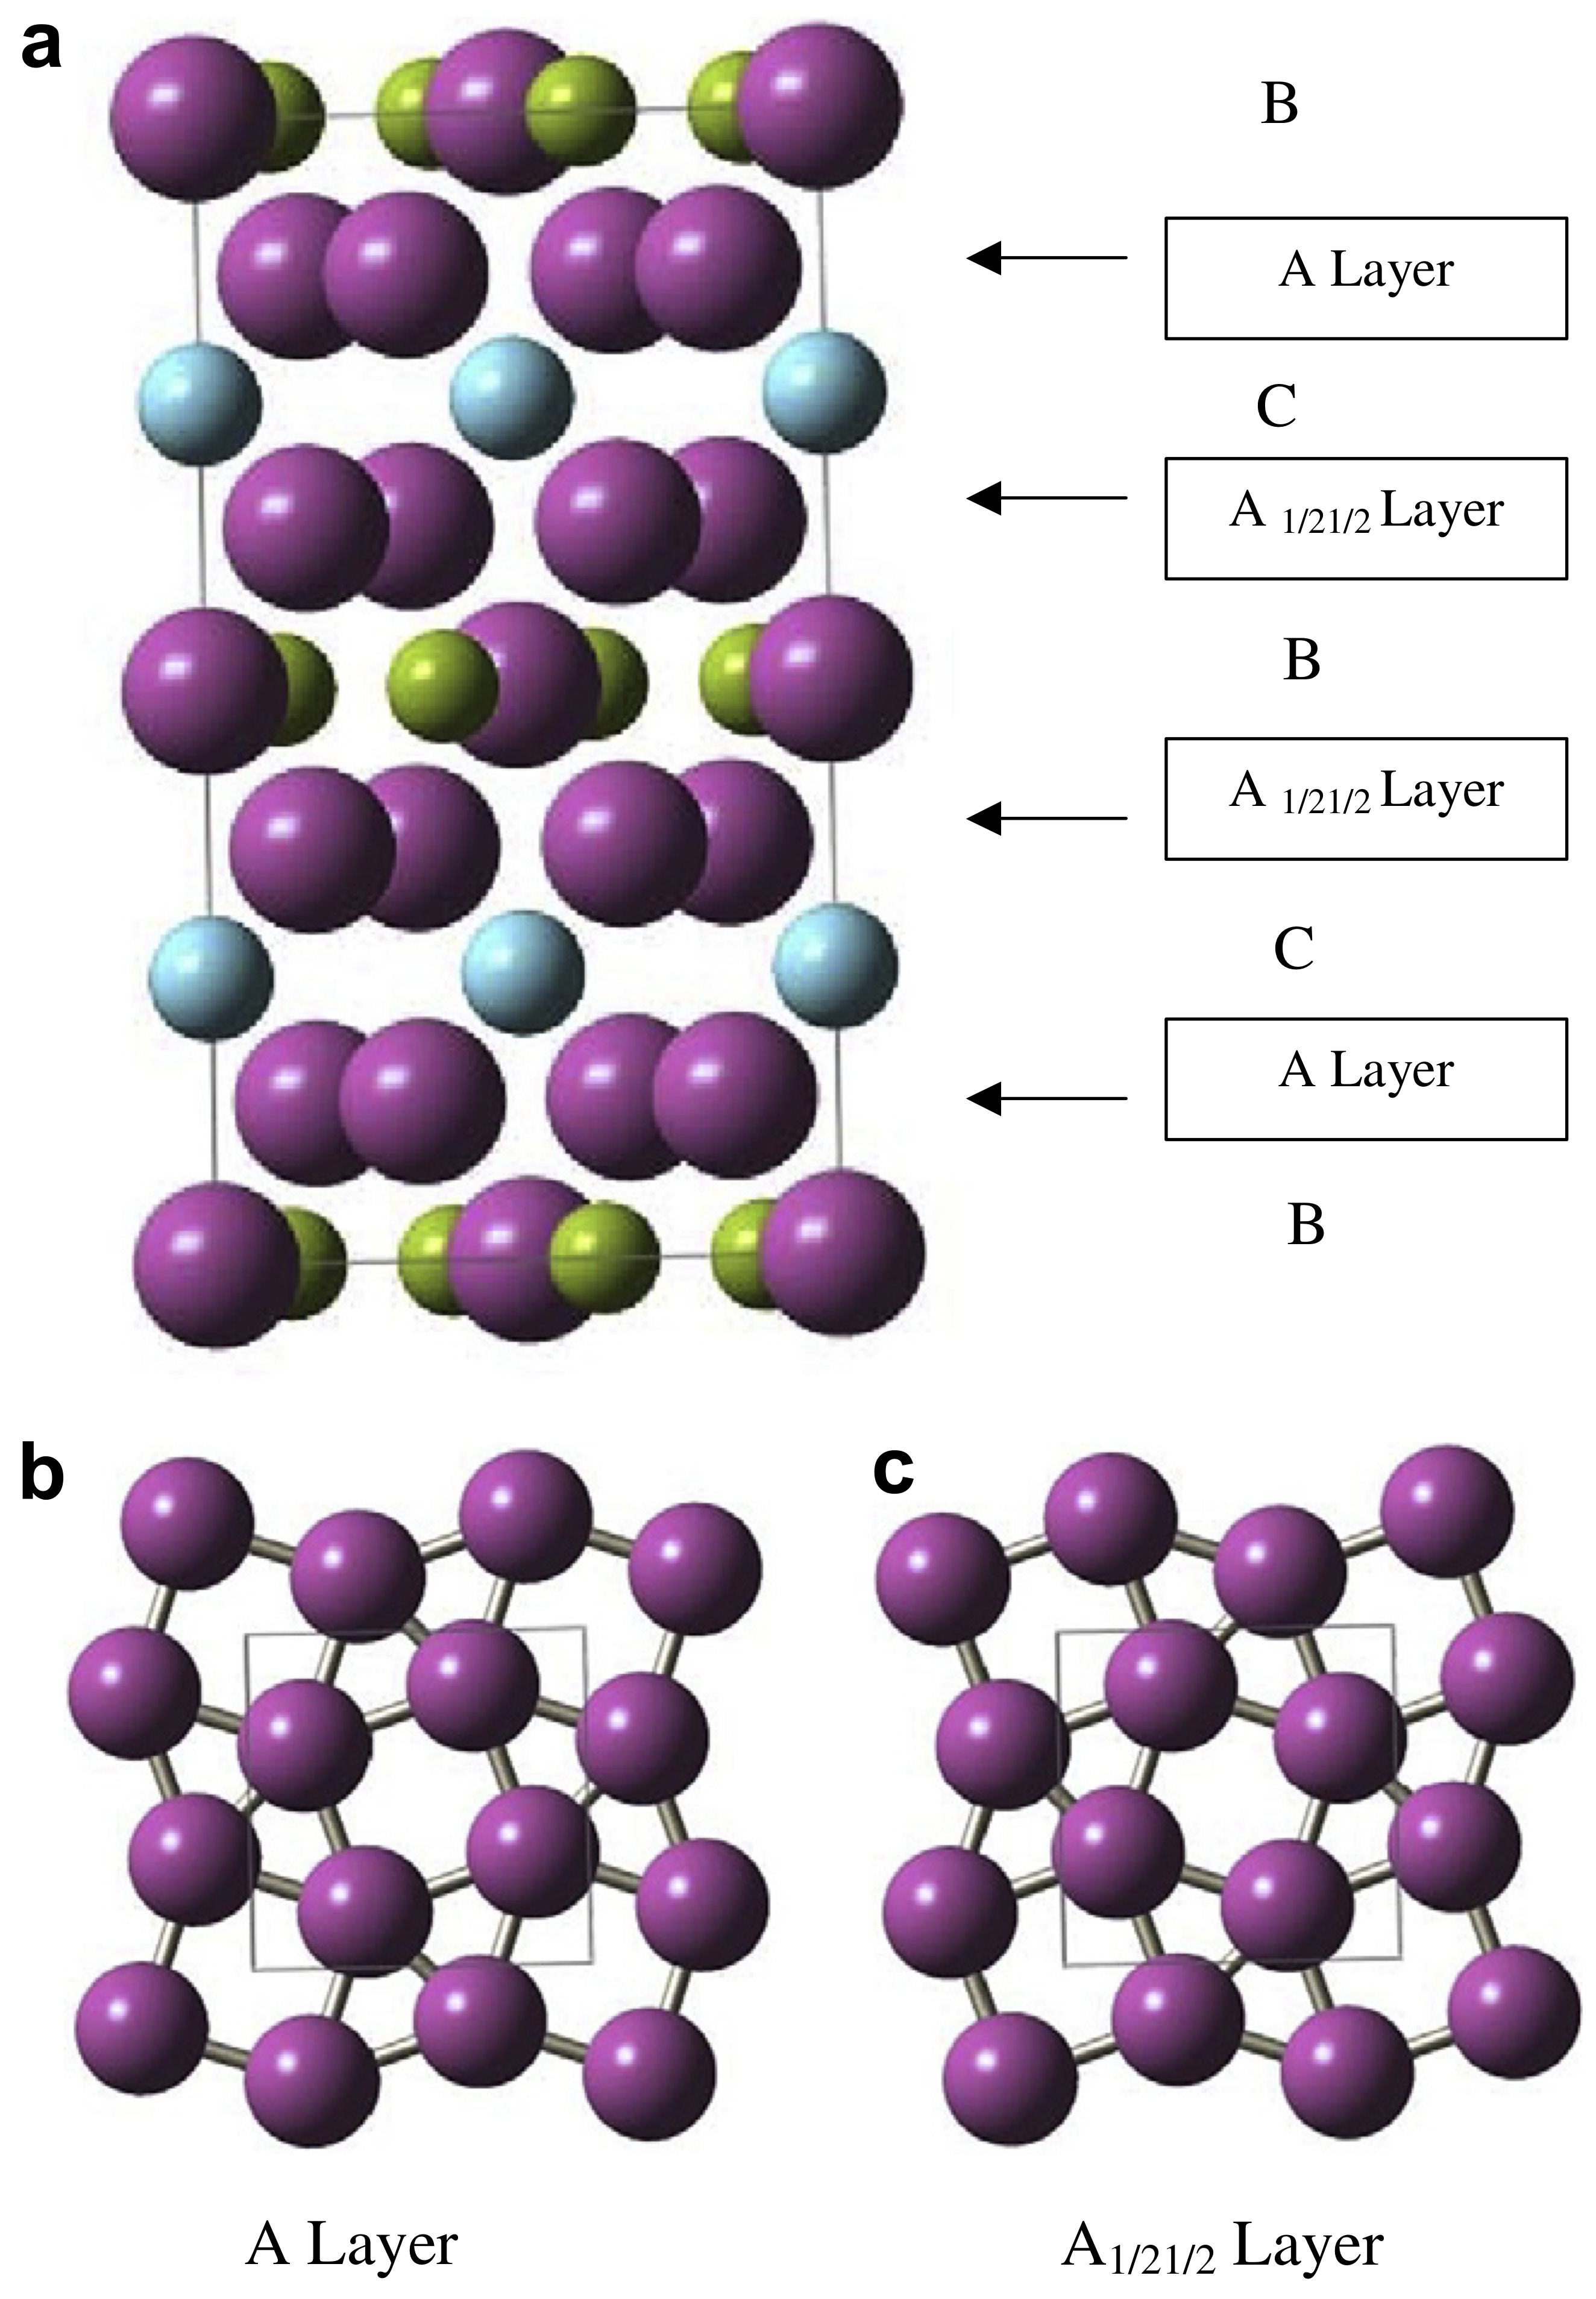
\includegraphics[width=9.5cm]{t2structure}
\caption{The crystal structure of Mo$_5$SiB$_2$ ~\cite{sakidja08}. }
\label{fig:T2structure}
\end{center}
\end{figure}
\vspace{-.2cm}
%
%
\begin{figure}[H]
\begin{center}
\includegraphics[width=\textwidth]{MoSiB_1600}
\caption{The ternary phase-diagram of Mo--Si--B ~\cite{nowotny57}.}
\label{fig:MoSiB_1600}
\end{center}
\end{figure}
%
%
\begin{figure}[H]
\begin{center}
\includegraphics[width=8.5cm]{Mo-Mo5SiB2}
\caption{Mo--Mo$_5$SiB$_2$ pseudo-binary phase-diagram ~\cite{yoshimi03}.}
\label{fig:Mo-Mo5SiB2}
\end{center}
\end{figure}
%
\clearpage
Nowotny et al. identified the T$_2$ phase in a 1600\celsius\ isothermal section of the ternary in 1957 (Figure \ref{fig:MoSiB_1600})  ~\cite{nowotny57}.  A Mo--Mo$_5$SiB$_2$ pseudo-binary phase-diagram has also been constructed by Yoshimi et al. (Figure \ref{fig:Mo-Mo5SiB2}) ~\cite{yoshimi03}.    An alloy of T$_2$ particles in a solid-solution matrix, when subject to compression-creep at different temperatures and strain-rates, show a range of deformation behaviour ~\cite{alur04}.  Brittle fracture, plastic deformation and elastic deformation were all observed.  

Perepezko has explored the influence of microstructure control in the manufacture of Mo--Mo$_5$SiB$_2$ and Mo--Mo$_3$Si--Mo$_5$SiB$_2$ for ultra-high-temperature applications (Figure \ref{fig:Mo16Si8B}) ~\cite{perepezko01}.  The ternary eutectic is difficult to attain via casting because solidification segregation causes very stable borides and silicides to form instead.  Also, the liquidus-surfaces for Mo$_3$Si and T$_2$ around the ternary eutectic region are shallow (Figure \ref{fig:MoSiB_liquidus}).  The invariant eutectic can be by-passed during non-equilibrium solidification.  Mo$_3$Si and T$_2$ would form instead, and there will be very little toughening component in the microstructure (Figures \ref{fig:Mo16Si8B} and \ref{fig:MoSiB_witheutectic}).

Perepezko has introduced alloying elements such as Nb to stabilise the T$_2$ phase and destabilise boride reactions (Figure \ref{fig:MoSiB_withNb}) ~\cite{perepezko01, sakidja00}.  Nb can substitute for Mo to a large extent in solid-solution and T$_2$.  This increases microstructural control and allows for direct solidification of a two-phase solid-solution and T$_2$ alloy in the region shaded in the liquidus-projection (Figure \ref{fig:Mo19Nb12Si8B}). 

%
\begin{figure}[H]
\begin{center}
\includegraphics[width=11cm]{Mo16Si8B}
\caption{SEM micrograph of arc-melted Mo--16.8Si--8.4B ~\cite{perepezko01}.}
\label{fig:Mo16Si8B}
\end{center}
\end{figure}
%
%
\begin{figure}[H]
\begin{center}
\includegraphics[width=14cm]{MoSiB_liquidus}
\vspace{-3mm}
\caption{The relevant portion of the Mo--Si--B liquidus projection T = 1873K ~\cite{perepezko01}.}\label{fig:MoSiB_liquidus}
\end{center}
\end{figure}
\vspace{-5mm} 	
%
%
\begin{figure}[H]
\begin{center}
\includegraphics[width=10cm]{MoSiB_witheutectic}
\caption{Microstructure of an alloy with T$_2$ as the primary phase with a Mo(ss)--T$_2$--Mo$_3$Si invariant ternary eutectic ~\cite{perepezko01}.}
\label{fig:MoSiB_witheutectic}
\end{center}
\end{figure}
\vspace{.7cm} 
%
\begin{figure}[H]
\begin{center}
\includegraphics[width=\textwidth]{MoSiB_withNb}
\caption{Increase in solid-solution volume-fraction in the ternary eutectic with Nb-alloying ~\cite{perepezko01}.}\label{fig:MoSiB_withNb}
\end{center}
\end{figure}
%
\begin{figure}[H]
\begin{center}
\includegraphics[width=9cm]{Mo19Nb12Si8B}
\caption{SEM micrograph of a polished section of cast and annealed Mo--19.5Nb--12Si--8.5B (at.\%) ~\cite{perepezko01}.}\label{fig:Mo19Nb12Si8B}
\end{center}
\end{figure} 
%

The dislocations formed in annealed alloys containing Mo$_5$SiB$_2$ are mostly of edge character with Burgers vectors of <100], 1/2<111], and <110], implying either that screw dislocations are far more mobile then edge dislocations and/or that the dislocations observed are formed from condensation of vacancies.  It has been suggested ~\cite{sekido07} that these vacancies are formed in Mo-rich alloys of Mo$_5$SiB$_2$.  The edge dislocations that form when these vacancies aggregate act as heterogeneous nucleation sites for subsequent Mo precipitation.  In Mo-lean Mo$_5$SiB$_2$, defects that form do not contribute to dislocation formation ~\cite{sekido07}.

%
\begin{figure}[H]
\begin{center}
\includegraphics[width=16cm]{sekido07}
\caption{ Weak-beam dark-field images showing dislocations in Mo-rich T$_2$ phase.  The specimen was annealed for 20 hours at 1550\celsius.  The Burgers vector of the dislocations are (a) [010] and (b) [-1-10􏰇] ~\cite{sekido07}.}
\label{fig:sekido07}
\end{center}
\end{figure} 
%

A Mo--Si--B alloy was measured to have fracture-toughness values of 8 \mega\pascal\,m$^{\frac{1}{2}}$ at ambient temperature, to 25 \mega\pascal\,m$^{\frac{1}{2}}$ at 1400\celsius\ ~\cite{alur06}.  This is higher than the 3 \mega\pascal\,m$^{\frac{1}{2}}$ reported for molybdenum silicide alloys without a toughening solid-solution phase.  The dominant creep mechanisms in this alloy were found to be grain-boundary diffusion between 900--1200\celsius, and volume diffusion between 1200--1400\celsius.

In recent work ~\cite{kumar10}, the tensile creep properties of HIP-manfactured Mo--Si--B alloys have been successfully evaluated.  Tensile tests at a creep-rate of 10$^{-4}$s$^{-1}$ between 1000\celsius\ and 1200\celsius\ were performed on a solid-solution alloy, a solid-solution and ~35vol.\% T$_2$ alloy, and a solid-solution, T$_2$ and Mo$_3$Si alloy (Figure \ref{fig:ku10}).

%
\begin{figure}[H]
\begin{center}
\includegraphics[width=7.8cm]{ku10i}
\includegraphics[width=7.8cm]{ku10ii}
\vspace{5mm} 
\includegraphics[width=7.8cm]{ku10iii}
\caption{Tensile stress-strain curves from tests conducted at a nominal strain-rate of 10$^{-4}$ s$^{-1}$, at temperatures between 1000\celsius\ to 1200\celsius\ for (a) an Mo solid-solution alloy with <5vol.\% T$_2$ phase, (b) a two-phase alloy with solid-solution and T$_2$ phase (35 vol.\% ), (c) a three-phase alloy with solid-solution, T$_2$ and Mo$_3$Si ~\cite{kumar10}.}\label{fig:ku10}
\end{center}
\end{figure} 
%

In other recent work, this X$_5$SiB$_2$ phase has been described as a common 5:3 metal--metalloid compound that exists in many systems ~\cite{sakidja08}.  It is present in the Nb--Si--B ternary ~\cite{nunes97}, the V--Si--B ternary ~\cite{rodrigues09}, the Co--Si--B ternary, the Fe--Si--B ternary, the Mn--Si--B ternary, and the (Pt, Ir, Rh, Ru)--Si--B  ternaries ~\cite{sakidja08}.  Cr, Ta, W, Ti, Zr and Hf are all soluble to varying extents in this phase ~\cite{perepezko01, sakidja00, sakidja05, sakidja08}.  There is an ``unusually large"  refractory metal solubility in the Mo sites in the T$_2$ phase ~\cite{sakidja08}.

The mechanical and oxidation properties of T$_2$-containing alloys from the Mo--Si--B system are promising.  There are several viable alloying additions that stabilise the T$_2$ phase and the solid-solution phase.  Some alloying additions destabilise undesirable boride phases and the X$_3$Si phase.  These factors allow a degree of freedom in subsequent multi-phase alloy design.  Prototype protective oxidation bond coats for these alloys have also been developed ~\cite{perepezko10}.  Kinetics and reactive diffusion pathway analysis have been utilised in the design of a borosilicide coating that has a multi-layer phase-sequencing that allows for thermodynamic compatibility and an underlying diffusion barrier between the bond coat and the underlying substrate ~\cite{perepezko10}.  During high-temperature exposure, the bespoke coating has been elegantly designed to evolve in such a way such that its life is prolonged.

The evolution of Mo--Si--B alloys over the last two decades illustrates that substantial progress can be made when a judicious, strategic alloy design approach is coupled with appropriate, bespoke testing.  These alloys can be reasonably considered as bench-mark alloys for high-temperature structural materials.



\subsection{Niobium Silicides}

Nb--Nb$_3$Si alloys have been the focus of much research, partly because of their low densities and good high-temperature mechanical properties, ~\cite{jackson96, fleischer87, fleischer94, sauthoff88, shah92, bewlay03, miura09, balsone01}.  These characteristics allow for greater design flexibility.  Niobium silicides have poorer oxidation resistance than their molybdenum counterparts, pesting at low and intermediate temperatures ~\cite{ramberg93}.  They have poor room temperature fracture-toughness.  These issues have yet to be resolved ~\cite{jackson96, fleischer87, fleischer94, sauthoff88, shah92, ramberg93, bewlay03, mitra06}.

There are three niobium silicides in the Nb--Si binary: Nb$_3$Si, Nb$_5$Si$_3$ and NbSi$_2$ (Figure \ref{fig:NbSi}).  Niobium has a density of 8.57  \gram\usk\centi\rpcubic\meter, and Nb$_3$Si has a density of 7.52  \gram\usk\centi\rpcubic\meter.  The eutectic between niobium solid-solution and Nb$_3$Si has been looked at ~\cite{kimura05}, but there are many phase transitions between room temperature and the eutectic melting point (Figure \ref{fig:NbSi}).  At 1765\celsius, Nb$_3$Si undergoes a eutectoid decomposition to Nb and Nb$_5$Si$_3$.  To further complicate matters, Nb$_5$Si$_3$ has two allotropes.  The high-temperature phase is D8$_{m}$, and the low temperature phase is D8$_1$.  D8$_1$ has high strength at elevated temperatures ~\cite{bewlay01}.  The transformation temperature ranges between 1650\celsius\ and 1940\celsius\, and varies with composition.  This makes the manufacturing process for the D8$_1$ phase more complicated.  These transformation temperatures are well above the target operating temperature of 1200\celsius.  Once manufactured, the D8$_1$ phase should be stable.

%
\begin{figure}[H]
\begin{center}
\includegraphics[width=12cm]{NbSi}
\vspace{-2mm}
\caption{The Nb--Si binary phase-diagram ~\cite{okamoto90}.}\label{fig:NbSi}
\end{center}
\end{figure}  
%

In a two-phase alloy of Nb solid-solution and $\alpha$--Nb$_5$Si$_3$,  dislocations developed in the intermetallic when the alloy was compressed at 1673K.  Three types of slip systems operating are: \{011\}<111], \{001\}<100] and \{010\}<100] ~\cite{sekido10}.

Hypoeutectic alloys have dendrites of Nb solid-solution with an inter-dendritic eutectic consisting of a Nb$_3$Si matrix with fine Nb rods and ribbons aligned with the primary growth direction.  Hypereutectic alloys were found to contain primary Nb$_3$Si and Nb$_5$Si$_3$ dendrites with inter-dendritic eutectic.  The fracture-toughnesses of these materials ranged from 5.8  \mega\pascal\usk\meter$^{\frac{1}{2}}$ at the eutectic composition to 14.2  \mega\pascal\usk\meter$^{\frac{1}{2}}$ for a hypoeutectic composition at 10 at.\% Si, which are significantly better than monolithic Nb$_5$Si$_3$ ~\cite{strum94}.  In fact, the fracture-toughness for the latter is close to the minimum threshold for fracture-toughness of 15 \mega\pascal\usk\meter$^{\frac{1}{2}}$ ~\cite{shah95}.  However, the addition of the niobium matrix decreases creep strength by an order of magnitude at 1200\celsius, with minimum creep-rates comparable to those of nickel-base superalloys.  

Specimens used in high-temperature structural testing are mostly made using HIP manufacture of powder.  Ingots have been successfully made through conventional DS manufacturing, with the help of minor Sn or Ag additions ~\cite{bewlay03, vellios10}.

The extent of oxidation resistance in niobium silicide alloys positively correlates with Si content ~\cite{xiong09}.  Oxidation kinetics for Nb--10at.\%Si and Nb--20at.\%Si were similiar at 1000\celsius\ and 1200\celsius; specimens experienced linear oxide growth rates.  Mo, Ta and W have been used as alloying additions that would contribute to high-temperature strength.  Nb--20Si--10W had a parabolic oxide growth rate, and its weight increase was only about a quarter of the Nb--Si alloys.  WO$_3$ formed during thermal exposure, and although it is oxygen permeable, it is less volatile than MoO$_3$.  This ternary alloy showed higher oxidation resistance than  the quaternary alloy Nb--20Si--10W--10Mo.  Al, Cr and Ti additions to Nb--Nb$_5$Si$_3$ improved oxidation behaviour, but oxidation growth rates remained linear even after 100 hours of isothermal exposure at 800\celsius\ ~\cite{zelenitsas06}.  The alloy that had 5at.\%Cr formed a very thick oxide layer (Figuree \ref{fig:zelenitsas}).  The thinner oxide layer that formed on the alloy containing all three element additions spalled off upon cooling (Figure \ref{fig:zelenitsas}b).  It still had a significant thickness of several \milli\metre.

%
\begin{figure}[H]
\begin{center}
\includegraphics[width=4.5cm]{zelenitsas}
\includegraphics[width=5.3cm]{zelenitsasii}
\vspace{-2mm}
\caption{ Photographs of Nb--Nb$_5$Si$_3$ alloys containing (in at.\%) (a) 5Cr and (b) 24Ti--8Cr--4Al that had been subjected to 800\celsius\ for 100h ~\cite{zelenitsas06}.}\label{fig:zelenitsas}
\end{center}
\end{figure}  
%

To improve oxidation resistance in Nb alloys, Shah has attempted to attain a microstructure of Cr$_2$Nb and Si in a Nb--Cr--Si solid-solution matrix to increase Si content in the alloy ~\cite{shah95}.  Results were not encouraging; this is believed to have been caused by a complex intersection of liquidus surfaces.  Bewlay has added Ti, Al, Cr and Hf to improve oxidation properties ~\cite{bewlay03}.

Niobium is an alloying element that can positively contribute to other metal-silicide alloy systems.  It improves oxidation behaviour in Ti-Al and Zr-based alloys ~\cite{zhan09}.  The (Nb,Mo)s.s.--(Nb,Mo)$_5$Si$_3$ eutectic system shows good high-temperature mechanical properties.  However, the issue of poor oxidation resistance has not been adequately addressed in this system.  


\subsection{Chromium Silicides}
%
There are four chromium silicides in the Cr--Si binary: Cr$_3$Si, Cr$_5$Si$_3$, CrSi and CrSi$_2$ (Figure \ref{fig:CrSi}) ~\cite{gokhale90}.  We are interested in Cr$_3$Si as our strengthening phase because it is the intermetallic that can co-exist with the BCC chromium solid-solution phase.  There has been some research conducted on Cr$_5$Si$_3$, and like other intermetallics that have not been ductile-phase toughened, it has been shown to be brittle at room temperature.  All phases of this binary have low density.  The density of the solid-solution, the densest phase, is 6.91  \gram\usk\centi\rpcubic\meter.  The density of the Cr-rich intermetallic, Cr$_3$Si, is 6.47  \gram\usk\centi\rpcubic\meter.  Both densities are substantially lower than nickel-based superalloys.  Cr is BCC (Figure \ref{fig:BCC}) and Cr$_3$Si is A15 (Figure \ref{fig:A15}).  

%
\begin{figure}[H]
\begin{center}
\includegraphics[width=.9\textwidth]{CrSi}
\caption{The Cr--Si binary phase-diagram.}\label{fig:CrSi}
\end{center}
\end{figure}
%
%
\begin{figure}[H]
\begin{center}
\includegraphics[width=7cm]{BCC}
\caption{The body centered cubic structure of the solid-solution ~\cite{ashcroft76}.}\label{fig:BCC}
\end{center}
\end{figure} 
%
The low density constituent phases in this binary allow for alloys to be designed with substantial solid-solution content.  Alas, utilising Cr solid-solution as a toughening phase in alloys is a rather difficult matter.  Cr is known to suffer from nitrogen-embrittlement and notch-sensitivity at ambient temperature.  This makes Cr-based alloys crack-prone, and they are difficult to manufacture using conventional casting techniques.  They are also difficult to process and machine.  Extensive research into alloying elements to decrease the ductile-brittle transition-temperature (DBTT) did not achieve DBTTs below room temperature (Figure \ref{fig:Cr_ductility}) ~\cite{abrahamson57}. Most precious group metals (PGMs) were not tried as alloying additions because of their high costs.  Cr's DBTT can be most effectively brought down to 40\celsius\ by 4-6at.\% additions of Ru.  This DBTT is not ideal as it is above room temperature.  Such high Ru content would substantially increase alloy density, material costs and alloy density. This would decrease the attractiveness of Cr-based alloys.


In a recent patent, Ag was described to be effective at plasticising Cr and allowed for 15\% tensile elongation in a Cr-Ag alloy. Yield strengths of Cr solid-solution containing 0.02--6.0at.\% Ag were measured at room temperature, and temperatures between 800--1200\celsius\ (Figure \ref{fig:crag}) ~\cite{gu07}.  At 1200\celsius, these Cr-Ag alloys have yield strengths of about 25 \mega\pascal.   At 800\celsius, a temperature below the DBTT of Cr, these alloys have yield strengths that increase with Ag content, lying between 70 \mega\pascal\ and 120 \mega\pascal.  In the Cr--Ag binary phase-diagram, it can be seen that Ag does not dissolve into Cr solid-solution.  The excess Ag probably forms precipitates within the Cr solid-solution.  These precipitates would be sites of weakness when a force is applied at high-temperature.  Ag has a low melting-point and would form little pools of liquid silver in the alloy at high temperatures.  

Cr$_3$Si has inferior high-temperature structural properties to Mo and Nb silicides ~\cite{fleischer89, mitra06}.  Alloying of Mo with Cr$_3$Si successfully provides high-temperature creep-resistance ~\cite{raj95a}, but resulted in poorer oxidation resistance ~\cite{tomasi97}.

%
\begin{figure}[H]
\begin{center}
\includegraphics[width=8cm]{A15}
\caption{The A15 structure of Cr$_3$Si ~\cite{nevitt95}.}\label{fig:A15}
\end{center}
\end{figure}
% 
%
\begin{figure}[H]
\begin{center}
\includegraphics[width=.98\textwidth]{Cr_ductility}
\vspace{-2mm}
\caption{Initial transition-temperature for 65$^\circ$ bend versus alloying addition (at.\%) ~\cite{abrahamson57}. }\label{fig:Cr_ductility}
\end{center}
\end{figure}
\vspace{-8mm}
%
%
\begin{figure}[H]
\begin{center}
\includegraphics[width=10cm]{crag}
\caption{Yield strengths of Cr solid-solution alloys with 0.2-6.0at.\% Ag, measured at room temperature, 800\celsius, 1000\celsius, 1200\celsius\ and 1400\celsius\ ~\cite{gu07}.}\label{fig:crag}
\end{center}
\end{figure}
%
\clearpage
The theoretical Cr$_3$Si volume fraction in the Cr--Cr$_3$Si eutectic is 42at.\%, as predicted by the binary phase-diagram (Figure \ref{fig:CrSi}).  Despite the brittle nature of the Cr solid-solution, research has been performed on this eutectic system.  The sensitivity of microstructure to changes in composition and solidification rate have been detailed by H.  Bei et al. (Figure \ref{fig:CrCr3Si _micros}) ~\cite{bei03a}.  Solidification rates can be used as a method for controlling microstructure.   When directionally solidified at 40mm/h, a beautiful lamellar eutectic microstructure forms due to a planar solidification front (Figure \ref{fig:DS_CrCr3Si}).  Slight deviations in composition of less than 1at.\% can cause the microstructure to regress from lamellar to cellular when manufactured by DS (Figure \ref{fig:funnel}).  A slow rate of 20mm/h can  allow off-eutectic compositions to grow in a lamellar fashion.  Faster rates are not as forgiving (Figures \ref{fig:degenerate} and \ref{fig:funnel}).

Raj reports Cr$_3$Si as having poor oxidation resistance above 1200\celsius\ ~\cite{raj95}.  When exposed for 4 hours at 1200\celsius, a Cr$_2$O$_3$ layer forms with islands of SiO$_2$ sitting on top.  After 4 hours at 1400\celsius, a layer of SiO$_2$ manages to form, but it possesses poor adhesion.  The silicon content is not high enough to allow the intermetallic to form a thin, protective silica layer.  When a critical oxide thickness is reached, greater residual stresses can build up that would cause the oxide layer to spall off during thermal cycling. 

%
\begin{figure}[H]
\begin{center}
\includegraphics[width=16cm]{ireallylovewill}
\caption{Changes in the microstructure of Cr--Cr$_3$Si with minute deviatiations from eutectic composition ~\cite{bei03a}.  All ingots were manufactured with the arc-melt process.}
\label{fig:CrCr3Si _micros}
\end{center}
\end{figure}
%
%
\begin{figure}
\begin{center}
\includegraphics[width=16cm]{DS_Cr-Cr3Si}
\caption{Cr--Cr$_3$Si eutectic alloy directionally solidified at 40 mm/h and 60 rpm: (a) transverse and (b) longitudinal sections ~\cite{bei03}.}
\label{fig:DS_CrCr3Si}
\end{center}
\end{figure}
%

%
\begin{figure}
\begin{center}
\includegraphics[width=16cm]{DS_Cr-Cr3Si_bad}
\caption{Cr--Cr$_3$Si eutectic alloy directionally solidified at (a) 40 mm/h and 60 rpm, and at (b) 150 mm/h and 60 rpm, transverse section, displaying cellular structure ~\cite{bei03}.}
\label{fig:degenerate}
\end{center}
\end{figure}
%
\begin{figure}[H]
\begin{center}
\includegraphics[width=14cm]{funnel}
\caption{Microstructures that evolve as a consequence of different solidification rates and slight variance in compositions ~\cite{bei03a}.}
\label{fig:funnel}
\end{center}
\end{figure}
%

%
\begin{figure}[H]
\begin{center}
\includegraphics{Cr3Si_alloying}
\caption{Effect of Ternary additions to the Cr$_3$Si phase field ~\cite{shah92}.}\label{fig:Cr3Si_alloying}
\end{center}
\end{figure}
\vspace{-5mm}
%

\clearpage
Hf alloying additions to Cr--Si have been investigated recently ~\cite{schoonover08}.  Hf improves high-temperature strength and  oxidation resistance ~\cite{yang09}.  The high-temperature variants of Cr$_5$Si$_3$ and Hf$_5$Si$_3$ are isomorphous and hexagonal.  There is complete solubility between them in a calculated liquidus projection.  This has been extrapolated from the thermodynamic data on both constituent binary systems.  A ternary eutectic reaction that formed Cr, Cr$_3$Si and Cr$_2$Hf was seen in an arc-melted ingot that was calculated to contain only (Cr,Hf)$_5$Si$_3$ (Figure \ref{fig:crhfsieut}).  Ingot manufacture with homogeniety and low compositional uncertainty was not achieved in this study.  This could have resulted in the ternary eutectic microstructure forming instead of the expected (Cr,Hf)$_5$Si$_3$ phase.  In a later study, it was proposed that this phase did not form because Hf substitution of Cr in chromium silicides is negligible ~\cite{yang09}.
 
%
\begin{figure}[H]
\begin{center}
\includegraphics[width=11cm]{crhfsi}
\caption{A calculated Cr–Hf–Si liquidus projection extrapolated from available thermodynamic data on the constituent binary systems.  Class I invariant reactions have been labelled ‘‘E’’, Class II reactions have been labelled ‘‘U’’, binary eutectic reactions have been labelled ‘‘e’’, and binary peritectic reactions have been labelled ‘‘p’’.  Arc-melt manufactured compositions have been labelled ‘‘AM’’ , and those labelled ‘‘IL’’ were melted using an induction-levitation melting system ~\cite{schoonover08}.}
\label{fig:crhfsi}
\end{center}
\end{figure}
%

%
\begin{figure}[H]
\begin{center}
\includegraphics[width=8cm]{crhfsieut}
\caption{ Microstructure of a Cr--Hf--Si ingot manufactured by the arc-melt process.  It contains a ternary eutectic, (a) Cr$_3$Si, (b) Cr solid-solution and (c) Cr$_2$Hf phase, but was calculated to contain only the (Cr,Hf)$_5$Si$_3$ phase ~\cite{schoonover08}.}
\label{fig:crhfsieut}
\end{center}
\end{figure}
%


\subsection{Vanadium Silicides}

There are four vanadium silicides in the V--Si binary: V$_3$Si, V$_5$Si$_3$, V$_6$Si$_5$ and VSi$_2$ (Figure \ref{fig:VSi}) ~\cite{smith90}.  The density of the solid-solution is 6.11 \gram\usk\centi\rpcubic\meter and V$_3$Si is 5.2 \gram\usk\centi\rpcubic\meter.  The V solid-solution melts at 1910\celsius\ and V$_3$Si melts at 1925\celsius\ ~\cite{freund78}.  Limited work has been done on V--V$_3$Si ~\cite{rostoker58, strum94}.

V$_3$Si retains its hot-hardness better than Cr$_3$Si (Figure \ref{fig:VCr_hardness}); it is over twice as hard as Cr$_3$Si at 1100\celsius\ ~\cite{shah92}.  Hot-hardness is a good indicator of high-temperature structural properties.  These two intermetallics are perfectly miscible (Figure: \ref{fig:Cr3Si_alloying}).  The creep performance of V$_3$Si is slightly better than Cr$_3$Si at 1200\celsius\ and 1400\celsius\ (Figure \ref{fig:creepshah92_2}).  Both phases are substantially less creep resistant than Cr-39Mo-23Si (black square), which is a single-phase X$_3$Si alloy of Cr and Mo.  Fracture-toughness was 10  \mega\pascal\m$^{\frac{1}{2}}$ in the arc-melted eutectic and above 20  \mega\pascal\m$^{\frac{1}{2}}$ in the induction-manufactured and DS manufactured eutectic alloys (Figure \ref{fig:vkic}) ~\cite{strum94}.  V--V$_3$Si alloys are tougher than other silicide alloys.  DS manufactured material with cracks propagating parallel to its growth direction was less fracture-tough (Figure \ref{fig:vfracture}).  Little ductile-phase extension was observed.  Crack-bridging is not a significant contributor to fracture-toughness; the rule-of-mixtures is more applicable in this system ~\cite{strum94}.

Chromium and vanadium form a perfectly miscible body-centered cubic solid-solution (Figure: \ref{fig:CrV}) ~\cite{kocherzhinskii85}, and alloying can decrease the number of ordered bonds to increase toughness.  The phase-diagram of Cr--V--Si is unavailable.

%
\begin{figure}[H]
\begin{center}
\includegraphics[width=12cm]{VSi}
\caption{The V--Si binary phase-diagram ~\cite{smith90}.}
\label{fig:VSi}
\end{center}
\end{figure}
%

%
\begin{figure}[H]
\begin{center}
\includegraphics[width=9cm]{VCr3Si_hardness}
\vspace{-2mm}
\caption{Hardness of Cr$_3$Si and V$_3$Si as a function of temperature ~\cite{shah92}.}\label{fig:VCr_hardness}
\end{center}
\end{figure}
\vspace{-1cm}
%



%
\begin{figure}[H]
\begin{center}
\includegraphics[width=16cm]{creepshah92_2}
\caption{Comparison of minimum compressive creep-rate of silicides and nickel superalloys versus stress between 1000--1400\celsius\ ~\cite{shah92}.}\label{fig:creepshah92_2}
\end{center}
\end{figure}
%


%
\begin{figure}[H]
\begin{center}
\includegraphics[width=16.5cm]{vkic}
\caption{Fracture-toughness of castings of V--V$_3$Si by the arc-melting (AM), cold-crucible induction-melting (IM) and cold-crucible directional solidification (DS) ~\cite{strum94}.}\label{fig:vkic}
\end{center}
\end{figure}
%
%
\begin{figure}[H]
\begin{center}
\includegraphics[width=15cm]{vfracture}
\caption{SEM fractographs of fractures (a) transverse and (b) longitudinal to specimen growth orientation ~\cite{strum94}.}\label{fig:vfracture}
\end{center}
\end{figure}
%
%
\vspace{1mm}
\begin{figure}[H]
\begin{center}
\includegraphics[width=10cm]{CrV}
\caption{Binary phase-diagram of Cr and V ~\cite{kocherzhinskii85}.}\label{fig:CrV}
\end{center}
\end{figure}
%

\subsection{Titanium Silicides}

There are five titanium silicides in the Ti--Si binary: Ti$_3$Si, Ti$_5$Si$_3$, Ti$_5$Si$_4$, TiSi and TiSi$_2$ (Figure \ref{fig:TiSi}) ~\cite{seifert96}.   Ti$_5$Si$_3$ has been found to have excellent density-corrected high-temperature properties, but, like other intermetallics, show poor fracture-toughness at room temperature.  It has a very high melting point of 2122\celsius.  The Ti-rich silicide, Ti$_3$Si, transforms to Ti$_5$Si$_3$ at 1167\celsius.  This transformation is strongly hindered by nitrogen and oxygen contamination ~\cite{costa10}.  The eutectic temperature between Ti$_5$Si$_3$ and Ti is 1340\celsius, which is very low. Although the density of the Ti solid-solution is very low (4.51 \gram\usk\centi\rpcubic\meter), it has a low melting point of 1667\celsius, and cannot be considered as a matrix for an alloy operating at 1200\celsius\ or higher. 

Ti$_5$Si$_3$ has a D8$_8$ hexagonal structure similar to Ta$_5$Si$_3$.  It has a high melting point of 2130\celsius, has a low density (4.32 \gram\usk\centi\rpcubic\meter), and has been found to possess good creep resistance and oxidation behaviour ~\cite{zhan09}.  It has a substantially smaller elastic modulus than TiSi$_2$ (Figure \ref{fig:creepshah92_3}).  Both Ti silicides have lower elastic moduli than MoSi$_2$ at temperatures up to 1000\celsius.

Substantial additions of Ti to the Mo--Si--B alloys have been found to enlarge the region of stability for three-phase equilibrium between Mo solid-solution, Mo$_5$Si$_3$ and the T$_2$ phase ~\cite{yang10}.  Ti mainly substitutes for Mo.

%
\begin{figure}[H]
\begin{center}
\includegraphics[width=14cm]{TiSi}
\caption{The Ti--Si binary phase-diagram ~\cite{seifert96}.}\label{fig:TiSi}
\end{center}
\end{figure}
%
%
\begin{figure}[H]
\begin{center}
\includegraphics[width=.8\textwidth]{creepshah92_1}
\vspace{-.3cm}
\caption{Measured elastic modulii of various silicide systems and nickel-base superalloys between room temperature and 1200\celsius\ ~\cite{shah92}.}\label{fig:creepshah92_3}
\end{center}
\end{figure}
\vspace{-.5cm}
%


\subsection{Tantalum Silicides}

Tantalum silicides have not been the focus of much research as a high-temperature structural material.  The metal-rich tantalum silicides are substantially denser than their molybdenum and niobium counterparts, and have similarly poor oxidation character.  The higher density and poorer oxidation are disincentives to work with Ta silicides.  Hexagonal close packed (HCP) tantalum has been used as an alloying addition in silicide development due to its potent solid-solutioning strength and high melt temperature of 3020\celsius\ ~\cite{schlesinger94, naidu90ta}.  Ta silicides occur as HCP Ta$_3$Si, Ta$_2$Si, Ta$_5$Si$_3$ and TaSi$_2$ (Figure \ref{fig:TaSi}).  The Ta-rich silicides have very high melting temperatures ranging between 2340--2550\celsius.  The eutectic between the Ta solid-solution and Ta--Ta$_3$Si has a very high melting point of 2250\celsius.  This is about 500\celsius\ higher than the eutectic melting temperatures of Cr-silicides and V-silicides.  

Ta additions to the Mo--Si--B alloys stabilise promote three-phase equilibrium between the solid-solution, the 5:3 silicide and the T$_2$ phase ~\cite{sakidja08}.

%
\begin{figure}[H]
\begin{center}
\includegraphics[width=12cm]{TaSi}
\caption{The Ta--Si binary phase-diagram ~\cite{naidu90ta}.}\label{fig:TaSi}
\end{center}
\end{figure}

 
\subsection{Tungsten Silicides}
Tungsten is a BCC metal that forms two silicides: W$_5$Si$_3$ and WSi$_2$ ~\cite{naidu90w}.  It is a very dense element (19.26 \gram\usk\centi\rpcubic\meter).  W$_5$Si$_3$ has the same crystal structure as Mo$_5$Si$_3$ and Nb$_5$Si$_3$; it is tetragonal. It has a very high melting point of 2320\celsius.  Its density is also very high, at 14.42 \gram\usk\centi\rpcubic\meter.  WSi$_2$ is quite dense (9.82 \gram\usk\centi\rpcubic\meter) and has a melting point of 2160\celsius.  Research on these silicides is sparse due to their high densities, poor fracture-toughness and poor oxidation behaviour.  Mo- and Nb- silicides are seen to offer better sets of properties.  W is used as alloying additions for these alloys.  Its addition to the Mo--Si--B alloys stabilise also promote three-phase equilibrium between the solid-solution, the 5:3 silicide and the T$_2$ phase ~\cite{sakidja08}.  WSi$_2$ has a very high Young's modulus of 470\mega\pascal\ at ambient temperature (Figure \ref{fig:creepshah92_3}), but data at higher temperatures has not been collected.


\begin{figure}[H]
\begin{center}
\includegraphics[width=12cm]{WSi}
\caption{The W--Si binary phase-diagram ~\cite{naidu90w}.}\label{fig:WSi}
\end{center}
\end{figure}


\section{Intermetallic Alloy Manufacture and Processing}

Intermetallics currently experience a low degree of microstructural refinement, as many have very high melting points above 2000\celsius.  The choice of casting equipment is limited for such materials; thus, a large portion of research has been performed on ingots that are arc-melted or processed by powder-metallurgy.  The fast solidification rates experienced by arc-melted ingots can result in micro-cracks caused by thermal shock ~\cite{raj95a}.  The presence of grain boundaries in these microstructures is disadvantageous for high-temperature creep-resistance.  On the other hand, the fine microstructure allows for effective load partitioning into the intermetallic phases.  Excellent creep resistances have been achieved in HIP-ped powder of Mo--Si--B ~\cite{kumar07, jain10}.

Arc-melted ingots are often used to assess alloy microstructure.  In this method, there is a very large distribution of cooling rates.  The bottom sample section will experience a rate of a thousand degrees a second as it lies next to the water-chilled copper hearth.  The top sample section is furthest away from the source of cooling, and will experience rates that, although considered high, are an order of magnitude lower.  Although lower rates may decrease residual stresses accumulated during cooling, the huge differential in cooling rates between the top and bottom of each specimen will induce residual stress in the specimen.  Fracture-toughness analysis would need to be carefully planned if any sensible, reliable data is to be obtained.  Otherwise, fracture-toughness testing on such non-ideal material would be merely testing the quality of material manufacture, or the magnitude of residual stresses present, and not the material’s intrinsic fracture-toughness.

It could be said that one should rather address the cause of the high differential of cooling rates instead of attempting to circumvent it.  Samples with such differentials will experience cracking during manufacture or machining, and cannot be used in mechanical testing of any sensible form.  To improve the machinability and fracture-toughness of silicide alloys, they must be cooled very slowly past their DBTT during manufacture.  Rates of 5 \celsius/minute or less would be ideal.  This way, internal strains due to the differential in phase CTEs will be minimised, if generated at all.  Single-phase silicides have been shown to possess no dislocations when cooled this way during casting by levitation melting.  This was accomplished by dropping the cast into an alumina crucible that was pre-heated to about 1200\celsius\ using an RF (radio frequency) heating coil.  This is a temperature that is definitely above the DBTTs of the alloys being cast.  The alloy was then slowly cooled from 1200\celsius\ to room temperature.  Without this modification of a pre-heated crucible, the alloys cast into a cool crucible have been known to violently explode into many pieces due to thermal shock.

Careful selection of eutectic compositions with melting points lower than 1750\celsius\ can allow these compositions to be cast using a radio-frequency furnace.  Polycrystalline DS or non-DS solidified ingots can be manufactured.  By having slow withdrawal rates, alloy microstructures can be controlled (Figure ~\ref{fig:plapp}).  For material that have melting points that are less than 2800\celsius, a mirror-image furnace can be used to cast poly-crystalline or single-crystal ingots.  Feed-ingot chemistry needs to be homogenous, growth and rotation rates need to be controlled to prevent orientation misalignment.

Shah has reported that material manufacture using this technique will prove experimentally difficult ~\cite{shah95}.  He also thinks that DS may not be sustainable for solid-solution rich or low viscosity melts.  This comment will prove to be prescient in this work.

%
\begin{figure}[H]
\begin{center}
\includegraphics[width=11.5cm]{plapp}
\caption{ A freeze-frame of a model of eutectic colony formation during directional solidification ~\cite{plapp02}.}
\label{fig:plapp}
\end{center}
\end{figure}
%




 %INPUT SILICIDE HALF
\section{Design Criteria}

Our pertinent criteria for alloys with the potential to supercede nickel-base superalloys have been drawn up using a representative 2$^{nd}$ generation nickel superalloy, CMSX--4, as a benchmark. We want creep and tensile properties to be an additional 100\celsius above CMSX--4. The material's density has to be less than 9.0 \gram\usk\centi\rpcubic\metre. Oxidation resistance needs to be an innate property, and an adherent thermodynamically stable, slow-growing oxide layer that has low oxygen permeability is required.  The three oxides that meet these criteria are those of chromium, aluminium and silicon (Figure \ref{fig:IntermetallicOxidation}).
%
\begin{figure}[H]
\begin{center}
\includegraphics{IntermetallicOxidation}
\caption{Parabolic growth constants of oxides on select ordered intermetallics.}\label{fig:IntermetallicOxidation}
\end{center}
\end{figure}
%
For alloys used at low to intermediate temperatures, chromium oxide is the preferred oxide as it has excellent corrosion resistance at this range of temperatures. Once placed in an environment with temperatures of higher than 1000\celsius, chromium oxide becomes thermodynamically unstable and volatilises. Thus, such alloys are inappropriate for use at high temperatures. Historically, alumina has been the oxide of choice for high temperature materials; however, aluminium-based intermetallics display mediocre high temperature mechanical properties. As for silicon-containing materials studies indicate that several systems possess good high temperature creep properties, but many systems still remain relatively unexplored. Silicon-containing systems will be explored to establish potential candidate systems to incorporate in our alloy design. 	

\section{A--A$_3$Si Alloy Design}
\subsection{Key Issues to Address}
Investigations of silicide-based high temperature alloys have focused on achieving creep resistant alloys at higher temperature capabilities than those of nickel-base superalloys. The low fracture toughnesses of 2--5 \mega\pascal\usk\meter$^{\frac{1}{2}}$ of monolithic intermetallics at room temperature, which is a fraction of a K$_{IC}$ of 15 \mega\pascal\usk\meter$^{\frac{1}{2}}$, the value that is generally agreed upon that is required for an alloy to be machinable ~\cite{raj95}. Due to the bonding nature of intermetallics and the existence of low energy cleavage planes, it will be difficult to improve fracture toughnesses substantially.

One approach to resolve this issue would be to introduce a toughening phase into the alloy.  For effective toughening, a continuous phase would be desirable ~\cite{kahn80}. By doing so, the load bearing area would effectively be reduced, and alloys of such a system would have lower creep resistances than intermetallic-intermetallic systems at a given temperature. Many intermetallic systems that are currently under investigation possess poor oxidative properties ~\cite{harris97}. One such system is the molybdenum - silicon binary.  Although all phases in this binary are susceptible to catastrophic oxidation at intermediate temperatures, their high temperature mechanical properties are being extensively researched. We do desire materials with higher temperature capability, but not at the expense of intermediate temperature properties. A turbine blade in an aero-engine's hot section experiences temperatures from 650\celsius\ at the blade base to 1100\celsius\ at the blade tip. Investigation of intermetallics in this system with higher silicon contents, such as MoSi$_2$, was undertaken in an attempt to increase the propensity for silica scale formation.  This compromised mechanical properties ~\cite{rawn01} and did not suppress pesting ~\cite{yanagihara96}. 

Tertiary elements such as Al were added on the basis that they had larger affinities to oxygen than Si and would be able to form a protective oxide layer.  However, Al has been added solely for its oxidative properties; extensive research on Al-based intermetallics have shown that they do not have good high temperature creep properties. This method is not ideal, as it compromises mechanical properties in order to improve oxidative properties, but fails to address other issues, such as the inherent low fracture toughness of such systems. 

The fact that arc-melted silicides with micro-cracks out-perform powder-processed ingots shows that the creep properties reported thus far are not an accurate reflection of the true potential of silicides.  This can be resolved provided production techniques can be developed. Designing alloys based on eutectic systems would lower the required casting temperature appreciably, and increase the likelihood of castability.  Low coeffficient of thermal expansion (CTE) anisotropy and high thermal conductivity can help minimise the extent of micro-crack formation during solidification.


\subsection{Silicide Selection}

To achieve effective damage tolerance, a toughening phase occurring as a continuous matrix is preferred over discrete particles.  By focusing our design efforts around eutectic systems that contain a solid solution phase, we seek to address two main issues.
\begin{enumerate}
\item Alloy microstructure can be designed with a continuous solid solution matrix.  \item Eutectics have substantially lower melting temperatures than the constituent intermetallics.
\end{enumerate}  
  This can allow increased ease of material manufacture and microstructural optimisation if the casting temperatures are lower than the maximum temperatures attain by existing or emerging equipment. There are only 10 A--A$_x$Si$_y$ silicide systems that contain a solid solution toughening phase and an intermetallic load-bearing phase, with a density of less than 9.0 \gram\usk\centi\rpcubic\metre. They must also have a high eutectic temperature that is higher than 1500\celsius, and have no phase transformation between room temperature and an operating temperature of 1200\celsius.  This reduces the number of candidates to Cr--Cr$_3$Si, Hf--HfSi$_2$, Mo--Mo$_3$Si, V--V$_3$Si and Y--Y$_5$Si$_3$, where the Cr, Mo and V systems have the same chemical formula A--A$_3$Si. The crystal structure of these two phases are shown in Figures \ref{fig:BCC} and \ref{fig:A15}. Basing the alloy design around the above three transition metal silicide systems is beneficial (Figure \ref{fig:periodictable}). 
%
\begin{enumerate}
\item Cr and V have low densities.
\item The A15 phase is cubic, which a simple crystal structure for an intermetallic.
\begin{enumerate}
\item it is more likely to possess sufficient equivalent independent slip systems.
\item it is more likely to permit plastic deformation at lower temperatures.
\end{enumerate}
\item Extensive alloying is possible because the formation of undesirable phases during will be minimised.
\begin{enumerate}
\item Cr and V are perfectly miscible.
\item Mo and V are perfectly miscible.
\item Cr$_3$Si and V$_3$Si are perfectly miscible.
\item Mo$_3$Si and V$_3$Si are perfectly miscible.
\end{enumerate}
\item All three systems have non-faceted/ non-faceted behaviour.
\begin{enumerate}
\item They form lamellar microstructures when solidified.
\item This increases fracture toughness.
\end{enumerate}
\end{enumerate}    
%
\begin{figure}[H]
\begin{center}
\includegraphics[width=4cm]{periodictable}
\caption{Portion of the periodic table showing the relative positions of Cr, Mo, Nb and V.}
\label{fig:periodictable}
\end{center}
\end{figure}
%
As mentioned, these systems have non-faceted/ non-faceted behaviour and form lamellar microstructures when solidified (Figures \ref{fig:growthmorphologies} and \ref{fig:DS_Cr-Cr3Si}) ~\cite{bei03}. The directionality of the lamellae can be controlled by directional solidification.  Slow solidification rates allow a planar growth front to be maintain, which allows for a neat lamellar structure to form. With fast solidification rates, the planar growth front breaks down, resulting in a cellular structure instead (Figure \ref{fig:DS_Cr-Cr3Si_bad}). The other scenario, non-faceted/faceted, is exemplified by nickel-base superalloys. They experience dendritic growth during fast solidification.
%
\vspace{1cm}
\begin{figure}[H]
\begin{center}
\includegraphics[width=.6\textwidth]{growthmorphologies}
\caption{Eutectic Growth Morphologies formed by planar and non-planar growth fronts.}\label{fig:growthmorphologies}
\end{center}
\end{figure}
%

\begin{figure}[hp!]
\begin{center}
\includegraphics[width=\textwidth]{DS_Cr-Cr3Si}
\caption{Cr-Cr$_3$Si eutectic alloy directionally solidified at 40 mm/h and 60 rpm: (a) transverse and (b) longitudinal sections ~\cite{bei03}.}\label{fig:DS_Cr-Cr3Si}
\end{center}
\end{figure}
%
\begin{figure}[hp!]
\begin{center}
\includegraphics[width=\textwidth]{DS_Cr-Cr3Si_bad}
\caption{Cr-Cr$_3$Si eutectic alloy directionally solidified at 150 mm/h and 60 rpm, transverse section, displaying cellular structure ~\cite{bei03}. }\label{fig:DS_Cr-Cr3Si_bad}
\end{center}
\end{figure} 
%
\begin{figure}[H]
\begin{center}
\includegraphics[width=9cm]{BCC}
\caption{The body centered cubic structure of the solid solution ~\cite{ashcroft76}.}\label{fig:BCC}
\end{center}
\end{figure} 
%
\begin{figure}[H]
\begin{center}
\includegraphics[width=9cm]{A15}
\caption{The A15 structure of A$_3$Si ~\cite{nevitt95}.}\label{fig:A15}
\end{center}
\end{figure}
Preliminary results show silicides with unoptimised microstructures containing micro-cracks display creep properties with a 200\celsius\ increase in temperature capability over nickel-base superalloys (Figures \ref{fig:creepshah92_1} and \ref{fig:creepshah92_2}.  However, these silicides have not been designed to contain a toughening phase and are very brittle, possessing poor fracture toughness at room temperature. 
%
\begin{figure}[H]
\begin{center}
\includegraphics[width=.6\textwidth]{creepshah92_1}
\vspace{-.3cm}
\caption{Compressive creep properties of candidate systems and nickel-base superalloys ~\cite{shah92}.}\label{fig:creepshah92_1}
\end{center}
\end{figure}
\vspace{-.5cm}
%
\begin{figure}[H]
\begin{center}
\includegraphics[width=.9\textwidth]{creepshah92_2}
\caption{Comparison of minimum compressive creep rate of silicides and nickel superalloys vs stress between 1000-1400\celsius\ ~\cite{shah92}.}\label{fig:creepshah92_2}
\end{center}
\end{figure}
%
\subsection{A--A$_3$Si Eutectics}

The first system to be assessed would be the Cr--Cr$_3$Si eutectic.  This eutectic system can help to counter the occurrence of ``pesting" as the character of chromium oxide is excellent for oxidation and corrosion resistances up to 1000\celsius ~\cite{raj95a}.  It is extensively used in alloy systems such as steel and nickel-base superalloys ~cite{reed06}. Cr is known to be a solid solution that is prone to nitrogen embrittlement and notch sensitivity ~\cite{abrahamson57}.  It is very sensitive to impurity content and its ductile-brittle transition temperature (DBTT) can range from 50--500\celsius\ (Figure \ref{fig:Cr_ductility}).  This can be most effectively brought down to 40\celsius\ through extensive alloying with ruthenium ~\cite{abrahamson57}.  This DBTT is not ideal as it is not below room temperature, and such additions would increase material costs and alloy density.
%
\begin{figure}[H]
\begin{center}
\includegraphics[width=.98\textwidth]{Cr_ductility}
\vspace{-2mm}
\caption{Initial transition temperature for 65$^\circ$ bend versus at.\% alloying addition ~\cite{abrahamson57}. }\label{fig:Cr_ductility}
\end{center}
\end{figure}
\vspace{-8mm}
%
Cr--Cr$_3$Si has the lowest melting point out of the 3 systems at 1705\celsius\ ~\cite{gokhale90}. The elastic constants of Cr$_3$Si have been reported by Bei et al.  to be between 98--412 GPa ~\cite{bei04}. Another system that will be looked at is the V--V$_3$Si eutectic.  Vanadium is tough; DBTT values between -110 and -65\celsius\ have been reported ~\cite{dunn61}. Data on the effect that vanadium has on the DBTT of chromium has not been found, but alloying vanadium with chromium can result in a solid solution with good room temperature fracture toughness. The creep performance of V$_3$Si is better than Cr$_3$Si at 1400\celsius\ (Figure \ref{fig:creepshah92_2}), and it retains its hot hardness better than Cr$_3$Si (Figure \ref{fig:VCr_hardness}). It is over twice as hard as Cr$_3$Si at 1100\celsius.  
%
\begin{figure}[H]
\begin{center}
\includegraphics[width=7cm]{VCr3Si_hardness}
\vspace{-2mm}
\caption{Hardness of Cr$_3$Si and V$_3$Si as a function of temperature.}\label{fig:VCr_hardness}
\end{center}
\end{figure}
\vspace{-1cm}
%
Chromium and vanadium form a perfectly miscible body-centered cubic solid solution (Figure: \ref{fig:CrV}) ~\cite{kocherzhinskii85}, and alloying can decrease the number of ordered bonds to increase toughness. The two intermetallics Cr$_3$Si and V$_3$Si are perfectly miscible as well (Figure: \ref{fig:Cr3Si_alloying}) ~\cite{shah92}. The phase diagram of Cr--V--Si is unavailable. This suggests that no additional phases will form if one were to move across the tie-line from eutectic Cr--Cr$_3$Si towards V--V$_3$Si, as Cr and V can completely substitute for each other. As there are no ternary phase diagrams available for the Cr--V--Si system, the location of the eutectic trough in ternary space will need to be determined.
%
\vspace{1mm}
\begin{figure}[H]
\begin{center}
\includegraphics[width=9cm]{CrV}
\caption{Binary phase diagram of Cr and V ~\cite{kocherzhinskii85}.}\label{fig:CrV}
\end{center}
\end{figure}
%
\begin{figure}[H]
\begin{center}
\includegraphics{Cr3Si_alloying}
\caption{Effect of Ternary additions to the Cr$_3$Si phase field ~\cite{shah92}.}\label{fig:Cr3Si_alloying}
\end{center}
\end{figure}
\vspace{-5mm}
%
As oxidation resistance needs to be an inherent property of a turbine blade material, a preliminary study of the oxidation behaviour of these tie-line eutectics needs to be conducted to determine which, if any, eutectic compositions has sufficient oxidation resistance. An alloy with sufficient oxidation resistance needs to form an adherent Cr$_2$O$_3$ layer at low and intermediate temperatures, and an adherent SiO$_2$ layer at high temperatures. This would probably result in a dual-layer oxide structure. It is suspected that substituting vanadium for chromium can result in a more oxidation resistant alloy, as all vanadium oxides volatise between 600--1200\celsius\ ~\cite{wriedt90}. During oxidation, and oxides of vanadium will undergo sacrificial oxidation and will not compete with Cr$_2$O3 and SiO$_2$ to form oxide layers. SiO$_2$ has the lowest parabolic rate constant out of Al$_2$O$_3$, Cr$_2$O3 and SiO$_2$, and decreasing chromium concentration can help prevent the oxidation of silicon from being overwhelmed by that of chromium during the onset of oxidation. SiO$_2$ could thereby have a better chance of forming a continuous layer. This can help combat the poor high temperature oxidation resistance of Cr$_3$Si reported by Raj ~\cite{raj95}. In the event that vanadium does not preferentially oxidise initially, a layer of vanadium-rich material will form just beneath the oxide layer. Upon oxide spallation, runaway may occur, as vanadium oxides are volatile and not protective. 

Shah reports that single crystal material is less likely to pest than material with uncontrolled coarse grain structure ~\cite{shah92}. He also states that single-crystal cubic intermetallics with isotropic CTE and low DBTT are not likely to pest, referring to his preliminary observations on Cr$_3$Si and CoSi$_2$. The pest effect was not investigated in the V-Si binary. Investigating the oxidation behaviour at intermediate and high temperatures of the eutectic compositions between Cr--Cr$_3$Si and V--V$_3$Si can verify if pesting is an issue.

%

\begin{figure}[H]
\begin{center}
\includegraphics[width=.78\textwidth]{shahpest}
\caption{Schematic map showing the effect of the DBTT, the nature of the grain structure and the anisotropy of the CTE on the pest effect ~\cite{shah92}.}
\label{fig:shahpest}
\end{center}
\end{figure}
\vspace{-9mm}
%
The temperature dependence of the alloys' specific weight change for a given exposure time may be presented as a way of ranking oxidation resistance. This will help clarify the effects of a Cr$_2$O$_3$ and SiO$_2$ dual-layer structure on oxidation properties. Due to the novel and intricate alloy manufacturing required, we need to determine whether we are able to reproduce the lamellar and cellular microstructures of Bei et al.. If successful, we will attempt to manufacture material of the same microstructure for the V--V$_3$Si eutectic. 

The effect lamellar spacing has on an alloy's high temperature mechanical properties will then be studied. It is suspected that cellular microstructures may exhibit better mechanical properties. With a smaller lamellar spacing, it will be more effective at crack deflection, and may even possess a spacing that is smaller than the critical crack length of the material, effectively toughening it through crack containment. Also, they are more anisotropic, and can better sustain impacts in the transverse direction. 

Several groups have reported that Mo substitutions for Cr in monolithic Cr$_3$Si result in improvements in both high temperature creep capabilities and resistance to runaway oxidation at low and intermediate temperatures ~\cite{raj95}. Since Mo and Nb sit beneath Cr and V on the periodic table (Figure {fig:periodictable}), limited substitution of Mo and Nb into the (Cr, V)--(Cr, V)$_3$Si system will be investigated as this may provide benefits to high temperature creep. There is a continuous A--A$_3$Si phase field in the Cr--Mo--Si system that extends across the Cr-rich side to the Mo-rich side, and additional phases should not form during addition of Mo.
\chapter{Alloy Manufacture}

It is well understood that the manufacturing route used to produce engineering components, especially for aerospace, is able to produce components with optimised properties and for this reason thermomechanical processing, despite its high cost, is preferred over casting in critical components.  In this chapter, we demonstrate that a robust route to manufacture is essential even at this early stage of development.  In this work, the lack of a robust route due to cost constraints has unfortunately been proven critical to the evaluation of these materials.  This chapter has been organised into: outlining the reasons for our choice in manufacturing routes, describing the non-directional and directional manufacturing routes explored, and summarising our findings in manufacture.

\section{Exploration of Alloy Manufacturing Routes}

Silicides are conventionally manufactured by hot isostatically pressing powder to achieve superior mechanical properties to arc-melted ingots.  This allows for a very fine, isotropic microstructure, and has been shown to result in effective load-partitioning into the intermetallic phase with the appropriate manufacturing conditions. 

Hot isostatic press is an expensive batch process, especially in the initial stages of experimental alloy design, where many alloys need to be explored empirically rather than designing many virtual alloys and manufacturing only one alloy.  It would have been ideal to process a representative base alloy of the explored system by both routes to determine the route that would produce a superior product.  Unfortunately, hot isostatic press manufacture was not pursued for several reasons.  A single batch of alloy powder would have cost thousands of pounds to make.  This would be a small batch of bespoke novel alloy, and there is a substantial probability that product quality could be questionable, seeing as the powder-producers would have no experience in milling this powder.  Grain size distribution would probably be wide.  The conditions required for hot isostatic press manufacture would need to be determined, as we have no experiences in pressing such powders.  The influence on powder quality and hot press conditions would be significant.  It was thought that the return on investment would not be high.  Hot isostatic press manufacture was thus not pursued as the main route of alloy manufacture.

DS manufactured eutectic alloy would have a lamellar microstructure which may improve fracture-toughness by increasing critical crack length through crack deflection.  Having the load-bearing intermetallic phase aligned along the loading-axis may be a good microstructure for withstanding load.

We thought it sensible to compare the mechanical properties of a base alloy manufactured through both directional solidified and hot isostatic press manufacture in the first instance to determine the superior route.  Due to limited funds and access to equipment, alloys could only be DS manufactured.  We will describe how this route of manufacture had limited success due to furnace limitations.


\section{Non-Directional Alloy Manufacture}

\subsection{Arc-Melt Manufacture} 

Arc-melt ingots were used in the initial exploration of potential compositions.  This method allows small, relatively isotropic ingots to be made up with ease, provided that the components are miscible, do not have vastly different melting points, and do not form intermediate phases that have very high melting points of above 2500\celsius.  

The in-house arc-melt machine available in-house is 20 years old and manufactured by Buehler.  It is operated by Mr Kevin Roberts, a technician that has decades of experience with arc-melting.  Ingots weighed between 15-45 \gram, and were slug-like, measuring 7-12 \centi\metre\ in length (Figure \ref{fig:crarc}).  After the first pass of the arc, ingots were flipped and re-melted twice more.

Most alloy melts flowed poorly under the arc.  Compositions containing chromium and silicon would crack into several pieces during the fast cooling rates typical of arc-melt manufacture (Figure \ref{fig:crarc}).  Adjacent grains in the ingots were found to possess vastly different microstructures, with one having a lamellar microstructure, and its neighbour comprising mostly of dendrites.  In some regions, unmelted bits of elemental stock were seen.  Silicon and silicides make for very viscous material that has poor mixability.  In other regions where unmelted stock is not seen, the non-lamellar microstructures may be a result of different undercooling rates experienced by a melt of eutectic composition.  For instance, if the degree of undercooling is too big, the melt will solidify into a melt containing pro-eutectic, as seen in Figure \ref{fig:dantzig}.

%
\begin{figure}[H]
\begin{center}
\includegraphics[width=10cm]{coolingrate}
\caption{Effect of undercooling on the microstructure of Al--Si alloys: (a) Eutectic composition, slow cooling, (b) euctectic composition, fast cooling, (c) hypereutectic composition, laser re-melted at 0.1\metre/s.}
\label{fig:dantzig}
\end{center}
\end{figure}
%
Regardless of whether the ingots are compositionally homogeneous, the ingots manufactured by the arc-melt process are intrinsically microstructurally inhomogeneous.  This cannot be homogenised or optimised in any reasonable fashion, and these ingots cannot be used for high-temperature mechanical testing of any sensible nature.  Besides, rampant sample cracking upon cooling from manufacture indicate that arc-melt material experience residual cooling stresses that are of substantial magnitude to cause catastrophic failure.  Even if an ingot did not crack during cooling, it would be prone to cracking during handling and machining.

%
\begin{figure}[H]
\begin{center}
\includegraphics[width=8cm]{crarc}
\caption{Photograph of a typical ingot manufactured by arc-melting that had cracked when cooled from manufacture temperature.}
\label{fig:crarc}
\end{center}
\end{figure}
%
It was thought that the vacuum system of the in-house arc-melt facilities may not be sufficient to prevent nitrogen-embrittlement of the ingots, which may contribute to the crack sensitivity.  There is no quick method to determine whether this was the case.  Manufacturing methods that produce higher ingot quality had to be explored. 

There is a National Laboratory with arc-melt manufacturing facilities located at Department of Materials Science at the University of Birmingham.  Compositions were sent in to Dr.  S. Koohpayeh at the facility to see if purer or more homogeneous samples can be achieved.  Due to the high viscosity of the material, smaller ingots weighing about 5-10 \gram\ were made.  The ingots manufactured had thinner cross-sections than alloys manufactured in-house at the University of Cambridge (Figure \ref{fig:bhamarc}).  This is probably due to higher temperatures achieved during manufacture, which allowed the alloy melt to flow quite well and would therefore result in better mixing.  Several batches of eutecitic alloys were made up, and had their microstructures examined.

%
\begin{figure}[H]
\begin{center}
\includegraphics[width=8cm]{bhamarc}
\caption{Photograph of an ingot manufactured by the arc-melt process at the National Laboratory at the University of Birmingham.}
\label{fig:bhamarc}
\end{center}
\end{figure}
%


\subsection{Radio Frequency Solidification Manufacture}

Radio Frequency ingot manufacture using a horizontal cold crucible was tried.  The chromium and silicon coupled very poorly with the RF field.  This meant that not all the feedstock melted.  The melt had very high surface tension, and would bead up.  Also, the vapour pressure of chromium was very high, and a substantial amount of chromium evaporated and condensed onto the inside surface of the water-chilled glass tube.  This meant that the resultant ingot composition would not be particularly close to the nominal composition.

The RF facilities of the Department of Physics, Cambridge, were used as an alternative to in-house alloy manufacture.  Identical manufacturing issues were encountered: incomplete melting of feed ingots, extensive vapourisation of chromium, poor coupling of feedstock and the RF field, and sample cracking during cooling from solidification temperatures (Figure \ref{fig:physicsrf}). 

%
\begin{figure}[H]
\begin{center}
\includegraphics[width=8cm]{physicsrf}
\includegraphics[width=8cm]{physicsrfii}
\caption{Photographs of a Cr--Cr$_3$Si arc-melt ingot that was melted in the horizontal RF furnace at the Department of Physics, Cambridge, and of the quartz receptacle that housed the ingot.}
\label{fig:physicsrf}
\end{center}
\end{figure}
%

\subsection{Graphite Furnace Manufacture}

Melting of alloys in a graphite furnace was attempted.  The graphite Astro$^{\textregistered}$ furnace used was built by Professor Bill Clegg, and can reach temperatures of up to 2400\celsius\ under vaccuum or in an inert atmosphere.  The intention was to cast homogeneous samples with equiaxed grains by bringing all of the feedstock substantially past its melting point to enable proper mixing, and cooling it down slowly so as to minimise the build up of residual stresses which may compromise the ingot's mechanical properties.  

A graphite pot of height 180\milli\metre\ and diameter 100\milli\metre\ was custom-made as a containment vessel in the furnace to contain the feedstock (Figure \ref{fig:cleanpot}).  Its interior surface was sprayed with a coating of boron nitride powder before every cast.  A notch was made into the lip of the pot to prevent its lid from being thrown off in the event of vigorous alloy volatilisation.  A boron nitride crucible with a very thin wall was custom-made to sit snugly inside this graphite pot.  Within this, crucibles of alumina and zirconia were used to hold the feed-stock.  In the event that a reaction were to occur between the alumina or zirconia crucible with the feedstock or melt, this would result in a failure of the crucibles to contain the melt.  Both the graphite pot and boron nitride layer would be in place to react with and contain the feedstock.  This protected the furnace from damage.

%
\begin{figure}[H]
\begin{center}
\includegraphics[width=7cm]{cleanpot}
\caption{Photograph of the graphite pot used as a containment vessel in the Astro$^{\textregistered}$ furnace.}
\label{fig:cleanpot}
\end{center}
\end{figure}
%

Arc-melt manufactured ingots were used as feed stock initially.  Cr--Cr$_3$Si was melted to determine its compatibility with alumina crucibles.  Alumina crucibles are relatively cheap, and maintain their integrity up to temperatures of about 1800\celsius, upon which softening occurs.  For runs that would experience temperatures of 1780\celsius\ or higher, zirconia crucibles would be appropriate.  Alloy-crucible compatibility would have to be established. 

The first run had a ramp of 20\celsius/minute to 1735\celsius, a temperature that is 20\celsius\ higher than the feed's theoretical eutectic temperature.  Only partial melting was achieved.  Perhaps the hot zone was not large enough to cause complete melting.  The large graphite pot may be acting as a shield against the radiative heating of the furnace.  Pots used to contain samples are generally thinner-walled and substantially smaller.  A run with the maximum temperature of 1760\celsius\ was set to see if complete melting could be acheived.  The resultant ingot was found to take the shape of the alumina crucible; however, two unmelted pieces of feed were found within the ingot.  Some porosity was seen, and many macro-pores were present, especially when melted in test-tube shaped crucibles (Figure \ref{fig:sponge}).  The melt was either too viscous to take on the shape of the alumina crucible, or was producing vapour that did not manage to escape due to the lack of a mechanism of stirring.  On the whole, also sample dimensions were uneven and small, the cast samples seemed to possess sufficient fracture-toughness.  This is probably due to the very slow cool through the DBTT of the alloy of about 20\celsius/minute, and shows higher sample quality than those produced by arc-melt manufacture.

%
\begin{figure}[H]
\begin{center}
\includegraphics[width=9cm]{spongei}
\includegraphics[width=6.36cm]{spongeii}
\caption{Photographs of two views of a sample made from arc-melt feedstock in a narrow zirconia crucible placed in the Astro$^{\textregistered}$ furnace.}
\label{fig:sponge}
\end{center}
\end{figure}
%
%
\begin{figure}[H]
\begin{center}
\includegraphics[width=9cm]{squat}
\caption{Photograph of the zirconia crucibles used in alloy manufacture in the Astro$^{\textregistered}$ furnace}
\label{fig:squat}
\end{center}
\end{figure}
%
The dimensions of crucibles used were changed from long, thin test tubes to squat, wide pots.  Squat pots would allow the melt to form into a suitably large and regular ingots more easily by reducing their surface area to volume ratios.  The intention was to produce enough suitable stock to manufacture homogeneous compression test specimens that could then be tested.  Arc-melt manufacture ingots were used as feed in these squat pots, and brought up to 1800\celsius\ at 20\celsius/minute, held for 15 minutes, and cooled at 20\celsius/minute.  This maximum temperature is high enough to melt the Cr$_3$Si intermetallic. Zirconia crucibles were used as they can withstand such high temperatures.  No significant reaction occurred between the ingot and the crucible.  Substantial vapour from the melt was found to have condensed on the inner surface of the graphite pot lid (Figure \ref{fig:dirtypot}a).  As zirconia crucibles are four times more expensive than alumina ones, when the option to use zirconia-coated alumina crucibles at a price that was equivalent to that of an alumina crucible, it was taken.  One such crucible was used for a Cr--Cr$_3$Si ingot, and was found to undergo a reaction  at temperatures under 1800\celsius, either with the feedstock or with itself (Figure \ref{fig:dirtypot}b).  The feedstock mostly evaporated during such conditions, possibly by forming intermediate compounds of lower melting points.

%
\begin{figure}[H]
\begin{center}
\includegraphics[width=7.8cm]{dirtypotlid}
\includegraphics[width=7cm]{dirtypot}
\caption{Photograph of the graphite pot after feedstock reacted with the crucibles in the Astro$^{\textregistered}$ furnace.}
\label{fig:dirtypot}
\end{center}
\end{figure}
%

Fine, granular stock of the alloys' elemental components was also used as feed.  Gaseous Cr that escapes from the melt coalesce and remain on the crucible wall, resulting in a sponge-like final product with some internal porosity.  When this granular feed was cold-pressed into pellets, porosity was slightly reduced, but the resultant ingot integrity was still insufficient.  Segregation due to large differences in element densities was also observed.  Si does not melt completely although it has a much lower melting point than the eutectic (Figure \ref{fig:CrSi}).  This is likely due to poor melt-mixing stemming from the lack of a mixing mechanism. 

All sensible combinations of variables for alloy manufacture have been done under an Ar atmosphere and under vacuum, but none has been successful.  High melt viscosity, the lack of a mechanism for stirring the melt, the differences in Cr and Si volatility, are some of the reasons.  This method was abandoned.


\subsection{Plasma-Melting}

Plasma-melting (PM) was pursued as alternative route of manufacture to arc-melting.  The National Laboratory at the University of Birmingham has a PM facility that can manufacture dome-shaped ingots weighing between 1.0--2.5 \kilogram.  This uses ionised argon gas to melt the feedstock which is contained in a hemispherical water-chilled copper hearth.  As there is no focussed heat-source in PM manufacture, the temperatures experienced by an ingot would be less than temperatures experienced during arc-melt manufacture.  Ideally, this would translate into less volatilisation of feed-stock, and greater homogeniety in the end product.  They are hemi-spherical and the cooling rates on the domed surface of the ingot are in contact with a water-chilled copper hearth, and are estimated to be of the same magnitude experienced by samples during the arc-melt process.  The cooling rates are much lower near the flat surface of the ingot due to the latent heat in the large ingot.  All samples except V$_3$Si exhibited cracking.  The high cooling rate differential experienced by the ingots.  Despite its superiority to the arc-melt method, it was not used as the primary method of alloy feedstock manufacture as there was an extensive waiting period of two years till the first chance to have ingots manufactured arose.

99.95\% purity Cr pellets, Si chips, V pieces, Ta pieces, W pieces, and Al pieces were used as feed.  The ingots weighed between 1.5--2.2 \kilogram, depending on the packing density of the feedstock used.  They were flipped and re-melted another three times each.  Two educated guesses of slightly different compositions were made for each of the binary alloys, in the hope that an ingot of each binary would have mostly lamellar eutectic.  Cr--Cr$_3$Si 15at.\%, Cr--Cr$_3$Si 16at.\%, V--V$_3$Si with 11at.\% Si and V--V$_3$Si with 13at.\% Si.  Then, \ilovewill{山}Ta, \ilovewill{山}TaAl (Figure \ref{fig:pmsantaal}), \ilovewill{山}W and \ilovewill{山}WAl were made.  The ternary eutectics were not manufactured.  This was deemed unneccessary as the arc-melted ingots, despite their inhomogenieties, showed continuous phase fields across both the solid-solution and the X$_3$Si  intermetallic. 

All ingots with the exception of V--V$_3$Si were susceptible to cracking during cooling and machining.  All ingots were cut with electro-discharge spark-machining.  Longitudinal cross-sections of all ingots showed pieces of remnant refractory metal (Ta and W) feedstock that remained unmelted (Figure \ref{fig:pmsantaii}a).  Transverse cross-sections taken near the flat surfaces of the ingots showed fragments of unmelted Si situated in a plane about 1  \centi\metre\ from the flat surfaces (Figure \ref{fig:pmsantaii}b).  The presence of substantial unmelted stock material is possibly be due to the high viscosity and surface tension induced by the high silicon and chromium contents. 



%
\begin{figure}[H]
\begin{center}
\includegraphics[width=7.8cm]{PMsanTaAl}
\includegraphics[width=7.8cm]{PMsanTaAlii}
\caption{Photographs of a \ilovewill{山}TaAl PM processed ingot displaying cooling cracks.}
\label{fig:pmsantaal}
\end{center}
\end{figure}
%
%
\begin{figure}[H]
\begin{center}
\includegraphics[width=7.8cm]{PMsanTaii}
\includegraphics[width=7.8cm]{PMsanWAlii}
\caption{Photographs of PM processed ingots of (a) \ilovewill{山}Ta and (b) \ilovewill{山}WAl displaying inhomogeneity.}
\label{fig:pmsantaii}
\end{center}
\end{figure}
%
%
\begin{figure}[H]
\begin{center}
\includegraphics[width=7.8cm]{PMsanW}
\includegraphics[width=7.8cm]{PMsanWAl}
\caption{Photographs of (a) \ilovewill{山}W and (b) \ilovewill{山}WAl PM processed ingots displaying through-specimen cooling cracks.}
\label{fig:pmsanw}
\end{center}
\end{figure}
%
\begin{table}[htdp]
\begin{center}
\begin{tabular}{llc}
\hline
Alloy 			&  Ingot Description		\\
\hline
Cr--Cr$_3$Si &cracked into several pieces, crumbly bits break off easily\\
V--V$_3$Si &minor crack in ingot, tough and not crumbly\\
\ilovewill{山}TaAl &minor cracks in ingot, tougher than Cr--Cr$_3$Si , not crumbly\\
\ilovewill{山}Ta &cracked into 7 pieces and crumbly bits chip off easily\\
\ilovewill{山}W &low surface tension, no meniscus, many cracks in ingot, not crumbly\\
\ilovewill{山}WAl &low surface tension, cracked into 4 pieces, not crumbly\\
\hline
\end{tabular}
\end{center}
\caption{Condition of as-cast ingots manufactured by the PM process.}
\end{table}




\subsection{Non-Directional Solidification Manufacture with the Vertical RF Furnace}

Arc-melt ingots were used as feedstock initially.  They were found to be inhomogeneous.  PM manufacture stock was used as feedstock in the newer specimens. 
 
Two castings of the Cr--Cr$_3$Si eutectic were done using the radio frequency furnace in Cambridge.  The first cast was allowed to equilibriate at 1740\celsius, 35\celsius\ above eutectic melting point, for 1 hour, before being withdrawn at 20 mm/h.  When the alumina crucible was broken open after the cast, the feed arc-melt ingot was found to have only partially melted.  The hold time was possibly not long enough for the ingot to melt, and the hot zone could be smaller than the feed ingot, and only the portion within the hot zone melted.  The second cast was equilibriated at 1780\celsius\ for an hour.  A better melt was achieved before this cast.  Peering down the opening of the cylindrical crucible, a meniscus was seen.  Under the circumstances, that was the best measure of the degree of melting of the feed ingot.  This ingot was also solidified at 20 mm/hr.  Due to reaction between the alumina crucible and cast ingot, the ingot had to be broken out of the crucible.  This ingot seemed to have been cast well.  Microstructural and compositional analysis have not been performed on the ingots yet, due to difficulties in getting the ingot cut.  The electro-spark machining equipment at the department were unsuccessfully employed.  The samples had to be out-sourced for machining.
%
\begin{figure}[H]
\begin{center}
\includegraphics[width=8cm]{rfsmall}
\caption{Photographs of a Cr--Cr$_3$Si arc-melt ingot that was non-directionally solidified in the in-house vertical RF furnace and experienced incomplete melting.}
\label{fig:rfsmall}
\end{center}
\end{figure}
%

\section{Directional Solidification Manufacture}

It was hypothesised that a lamellar microstructure aligned to the loading axis would be able to partition load to the silicide phase effectively.  In order to accomplish this, pull-rates have to be very low to maintain the suitable growth front required.  This invariably leads to microstructure coarsening.  The various attempts at DS met with limited success due limitations of temperature capability, the lack of a mixing mechanism for the melt, and the lack of homogeneous feed-stock.  


\subsection{Directional Solidification with the Vertical RF Furnace}

Zirconia-coated alumina crucibles were also tried, with a maximum casting temperature of 1760\celsius.  This is a temperature that alumina can withstand without adverse effects.  The crucible underwent a reaction with itself at 1760\celsius.  The crucible lip, which was not in contact with the feedstock, melted, splitting and curling downward.  A small piece of the alumina crucible holding this compromised crucible chipped off, and hit the water-chilled double-walled silica containment vessel.  This alumina piece was at a temperature close to 1760\celsius, and its impact with the inner silica wall induced sufficient thermal shock to initiate the catastrophic failure of the silica vessel.  A bespoke replacement of the silica vessel had to be made before the furnace could come back on-line.  This process took three months.

%
\begin{figure}[H]
\begin{center}
\includegraphics[width=10cm]{rfi}
\caption{A photograph of a typical directionally solidified cast cylindrical specimen manufactured using the in-house vertical rf furnace.}
\label{fig:rfia}
\end{center}
\end{figure}
%

The recommended maximum operating temperature of the in-house RF furnace is 1800\celsius.  In order to preserve the life-time of the furnace, it has never been run at temperatures above 1600\celsius.  We were hesitant to push it to the maximum recommended temperature as the temperature is controlled manually.  If sudden runaway temperature increases occur, there will not be an automatic cut in power to curtail the temperature ramp. Exceeding the maximum temperature would be probable if feedstock had to be melted at 1800\celsius, especially since furnace temperature fluctuations are greater at higher temperatures.  Although we readily discovered that 1760--1790\celsius\ was insufficient to completely melt feedstock, furnace fluctuations of 40\celsius\ proved difficult to control at 1800\celsius, and only two or three ingots were manufactured at this temperature.  The RF furnace has a definite hot zone, and an initial pass of the feedstock through this hot zone was incorporated into subsequent alloy manufacture attempts, as much as the furnace constraints would allow.  

DS \ilovewill{山}W (Figure \ref{fig:sanw})  manufactured using the in-house RF furnace has a very high melting point.  The 1780\celsius\ capability of the RF furnace was not high enough to induce sufficiently low melt viscosity to allow the composition to solidify as a rod.
%
\begin{figure}[H]
\begin{center}
\includegraphics[width=9cm]{santarf}
\includegraphics[width=6cm]{santarftop}
\caption{(a) the long view of an ingot of \ilovewill{山}Ta by DS manufacture using the in-house RF furnace, made with PM manufactured feed-stock. This was melted at about 1785\celsius\, drawn at 30milli\metre\/h to melt and somewhat homogenise the feedstock, and re-drawn at 30\milli\metre\/h.  (b) the top view of the ingot, showing unmelted feedstock due to limited furnace temperature capability.}
\label{fig:santarf}
\end{center}
\end{figure}
%
%
\begin{figure}[H]
\begin{center}
\includegraphics[width=10cm]{sanw_arc}
\caption{(a) An arc-melted ingot of \ilovewill{山}W using PM-manufactured feedstock.  It broke into several pieces on the water-chilled hearth when cooling down from melt temperature.}
\label{fig:sanw_arc}
\end{center}
\end{figure}
%

%
\begin{figure}[H]
\begin{center}
\includegraphics[width=10cm]{sanw}
\caption{(a) the long view of an ingot of DS manufactured \ilovewill{山}W using the in-house RF furnace, made with PM manufactured feed-stock. This was melted at about 1780\celsius\ and drawn at 30milli\metre\/h. Part-way through the cast, the thermocouple broke, and the furnace was run at maximum capacity to increase the chances of a successful cast.}
\label{fig:sanw}
\end{center}
\end{figure}
%


\clearpage
\subsection{Four-Mirror Image Furnace Manufacture}

Several casts was performed using the 4-mirror furnace at the Physics Department of the University of Warwick (Figure \ref{fig:MirrorFurnace}).  This method of casting has been successfully used to manufacture single-crystal single-phase intermetallics and ceramics.  A homogeneous, single-phase feed ingot with a circular cross-section is required.  Feed ingots are typically made via the arc-melt process or through pressing powders.  The seed ingot needs to be single-crystal to manufacture single-crystal material.  

This method has not been successfully used to manufacture eutectic alloys.  Slight deviations from eutectic composition in the feed ingot would result in substantial temperature fluctuations in the melt.  If the composition being melted has a too high of a melting point due to the presence of primary dendrites, the melt volume would shrink and contact between the feed ingot and seed ingot would break. 
 

The casting rate was at the furnace's maximum drawing rate of 18 mm/h.  Despite using an ingot that had undergone several arc-melts, inhomogenities still persisted, and the melt could not be sustained as the melting temperature of the feed ingot fluctuated too much.  Due to the unstable nature of casting inhomogeneous eutectic alloys, the melt broke three times.  Although melt contact was re-established each time, this meant that the grains were discontinuous, and there is not enough uninterrupted length to machine out a creep specimen (Figure \ref{fig:FirstCast}).

At this casting rate, a lamellar microstructure should be seen.  However, there is too much dendritic chromium solid-solution pro-eutectic in the microstructure disrupting lamellae formation.  Only about 2\% of the area fraction of the transverse section was lamellar. 
%
\begin{figure}[H]
\begin{center}
\includegraphics{MirrorFurnace}
\caption{Photograph of the 4-mirror furnace at the University of Warwick.}
\label{fig:MirrorFurnace}
\end{center}
\end{figure}
%
%
\begin{figure}[H]
\begin{center}
\includegraphics{mirroron}
\caption{Photograph of the 4-mirror furnace in operation.}
\label{fig:MirrorFurnace}
\end{center}
\end{figure}
%

%
\begin{figure}[H]
\begin{center}
\includegraphics{FirstCast}
\caption{Photograph of the first directionally solidified Cr--Cr$_3$Si ingot.}\label{fig:FirstCast}
\end{center}
\end{figure}
%





\chapter{Microstructure and WDS Analysis of the X--X$_3$Si Alloys}

The aim of Wavelength Dispersive Spectrometry (WDS) analysis is to gather more reliable evidence in order to provide an explanation of microstructures seen.  Many of the alloys were initially assessed by optical microscopy and SEM/EDS.  This has been briefly described in the previous chapter.  It was difficult to interpret the EDS data collected, as there were too many uncertain factors to draw any worthwhile conclusions.

The WDS data was collected using five detectors that can each be assigned to collect several specific wavelength ranges corresponding to the waves emitted by an element.  Collected wavelength ranges can be selected such that any overlap of peaks from different elements is eliminated.  When performed correctly, accuracy of WDS data can be within a narrow range of 100 $\pm$0.1wt.\%.  

We present the binary and ternary alloys as a set in the first portion of this chapter, and the quaternary and quinary alloys as a set in the second portion.
%\ref{section:Microstructure of Quinary \ilovewill{山}WAl}. 
In current literature, only binary phase-diagrams of the binary alloys are available.  We seek to:

1.  Expand existing phase-diagram knowledge in the ternaries, quaternaries and quinaries explored in this project.

2.  Examine the extent to which solidified alloys reflect consistent equilibrium compositions, and demonstrate that  compositional variation within each ingot illustrate that mobility is very difficult across these systems.

The various microstructures presented in this Chapter will be summarised in Conclusions, together with any suitable mechanical data that can be used.

\section{Calibration, Set-up and Method of WDS Data Collection}

Prior to WDS analysis, simulations were run in simulation software ``Virtual WDS" to help determine the experimental set-up for optimal data acquisition.  This software allows us to avoid the majority of situations that produce results of poor quality by selecting the K, L and M lines of elements used such that they do not overlap and interfere with each other.  Empirical observation then allows us to modify the parameters of non-ideal data acquisition situations, but may not improve data quality.  

A 20nA beam was used to obtain better collection statistics and better minimum detection levels.  Frequent calibration using silicate and pure element standards ensured sound data, and only measurements that fell within 100.0$\pm$0.8 total weight percent were taken.  Peak profiles collected for each elemental standard were used to specify the range of wavelengths to be collected for each element in the alloys.  Ideally, the peaks with the strongest signal were chosen.  However, if any peak selected for collection overlapped with another, weaker peaks for the elements involved would have to be selected instead.  This would minimise data collection inaccuracies.  Overlap typically occurred with elements that are next to each other on the periodic table, such as tantalum and tungsten.  In order to obtain statistically reliable data, 10 seconds was spent collecting the background signal of each peak, and 20 seconds was spent collecting the signal from each peak.  Si has some overlap with Ta and W. 

A typical method for obtaining bulk eutectic compositions would be to get an area scan made up of adjacent line scans.  Large areas of 100-200\micro\square\metre\ could be analysed by having consecutive line scans performed within the selected region.  Such line-scans would make rapid passes along the selected area, spending micro-seconds at each point along the pass.  The line-analysis data collected would have inferior statistics to spot-analysis.  Alternatively, the WDS set-up could be configured such that the beam spot size is very large, with a diameter of 100\micro\metre.  The maximum diameter of beam striking the sample surface is controlled by the working distance between sample surface and where the beam is last influenced by the electromagnetic coils, and also the strength and range of the electromagnetic coils used to deflect the electron beam.  When performing WDS, working distance is typically standardised to 15 \centi\metre.  If working distance was increased to increase beam size on the sample surface, calibration will have to be performed at this working distance.  Regardless of whether a change of working distance is implemented, the beam striking the sample surface could thus be a lot smaller than 100\micro\metre\ and measuring it would be a protracted process.  It is difficult to determine the exact dimensions of the area being analysed when the diameter of the beam is set up to be overly large.  The alternative of increasing the working distance would involve recalibration of the WDS to the new working distance.  This process would be non-trivial, and was deemed unnecessary to pursue.

It was decided that the most sensible method to determine alloy mean compositions was to measure grids of 5x5 to 10x10 of large 10-20\micro\metre\ spots.  These grids make the data collected statistically random.  In alloys where insufficient eutectic area fraction translate to small regions of eutectic, grid analysis cannot be performed.  Instead, the spots had to be site specific to prevent any interference from dendrites.  The spots were large enough to cover a substantial area, but small enough to accurately determine the location and dimensions of the area analysed by each spot.  A large inter-spot distance was placed between spots to prevent any sample volume from being part of more than one analysis.  This distance of 15--50\micro\metre\ would scale with spot size, with the aim to minimise analysis of a volume that had already been compromised by the electron beam.  Averaging the results obtained, after removing outliers, would give an alloy’s average composition.  A microstructure may be eutectic on the sample surface, but there may be a dendrite of one phase lying right beneath the surface.  This would result in a distinctly non-eutectic composition, which would skew the average composition.  We will find that obtaining average compositions would oversimplify the data, and that it would be more illustrative to provide a composition range for each alloy. 

1\micro\metre\ spot analyses of the individual phases were performed only on the DS alloys, as the lamellar spacing of the non-DS alloys were too small to provide sufficient analysis volume for accurate measurements.  
The distribution of measured compositions has been shown in a composition map (Figure \ref{fig:ternarymap}).  The five alloys measured have compositions which span the full range between Cr--Cr$_3$Si and V--V$_3$Si, as in the case of Figure \ref{fig:WDSaveragecompo}.  These plots reflect tie-lines in the phase-diagram.  All alloys followed the same trend of having an X$_3$Si phase with 19--23 at.\% Si, and a solid-solution phase. The bulk eutectic compositions lie between 9--16at.\%Si.  
Why is there a large range of 3-10at.\% Si in measured bulk eutectic compositions? Melts that deviate slightly from eutectic composition are guided down a solidification trough to the eutectic point, where the rest of the alloy solidifies at a specific composition.  The following is a summary of possible explanations:

Case 1.
There may be dendrites present very near the analysed surfaces due to the difficulties in achieving alloy manufacture of high quality, where homogeneous ingots would comprise of at least 95\% volume fraction of lamellar microstructure.  Instead, rampant dendritic growth was present in the majority of alloys explored.  Alloys systems in which dendritic growth could be curtailed are \ilovewill{山}W, \ilovewill{山}WAl.  Dendrites, being composed of one phase only, would skew the collected data away from the euctectic composition, and towards its composition.  This leads to a larger range of compositions measured even if the eutectic microstructure has a very narrow composition range.  Unfortunately, minimising the occurrence of dendrites was very difficult with the routes of manufacture pursued in this project.

%
\begin{figure}[H]
\includegraphics[width=16cm]{ternarymap}
\caption{ WDS-measured eutectic, solid-solution and X$_3$Si compositions collected for the five binary and ternary alloys plotted in a ternary map.}
\label{fig:ternarymap}
\end{figure}
%
%
\begin{landscape}\vspace*{\fill}
\begin{figure}[H]
\begin{center}
\includegraphics[width=24cm]{WDSaveragecompo}
\caption{Composition map of average bulk eutectic compositions and phase individual compositions of the five binary and ternary alloys.  Average bulk eutectic compositions were measured for non-directional-solidification manufacture ingots using a statistically random method.  Average individual phase compositions were measured in DS manufactured alloys only, as the lamellar spacing of arc-melt manufactured alloys were too small to provide sufficient analysis area for accurate measurements.}
\label{fig:WDSaveragecompo}
\end{center}
\end{figure}
\end{landscape}
%


Case 2.
The high viscosity of the melt means that a lamellar microstructure may grow into the melt with an equilibrium composition and equilibrium phase fraction, while rejecting unsuitable elements into the remaining melt.  The remaining melt then has to solidify with phase fractions that are atypical of eutectics at equilibrium.  The eutectic microstructure inherently has a large composition range.

Case 3. 
There were discrepancies in measured data due to the conditions in which composition measurements were performed.  The eutectics have a narrow composition range, but due to the interactions between the transition metals and silicon, accurate measurements cannot be made without bespoke intermediate WDS standards being used.  This issue has been raised by other scientists working on silicides. 

When determining potential peak overlaps using a simulation software package "virtual WDS",  the majority of overlapping peaks are found.  The output of this package is used to construct set-up file that detail the initial WDS acquisition conditions that would be evaluated for suitability, and reconfigured as required.  

Initially, WDS calibration was done with pure element standards at the start of the day.  Cr, Si and V were used for the binary and ternary alloys.  Measurements of the solid-solution phase would usually sum up to 100at.\%.  Measurements of the silicide phase were unreliable.  They consistently totalled to less than 100at.\%.  It was thought that interactions between Si and the transition metals in the alloys played a part in measurement inaccuracy. 
 
An intermediate standard, calcium fayalite, was then used.  This is a silicate containing calcium.  It was found that the measured total weight percent was less accurate than using element standards, and measured 96--98\%.  Repeated re-calibration with calcium fayalite showed that the WDS machine was consistently producing very accurate measurements of 100.0$\pm$0.3at.\% with different spot sizes and beam current intensities.  This suggests that an unknown interaction within the investigated silicide alloys is contributing to measurements consistently totalling less than 100\%.  An intermediate standard iron fayalite was tried.  Iron is a transition metal, and any interactions between transition metal and silicon would be accounted for when using iron fayalite as a standard.  Iron fayalite measurements fell within 100.0\% $\pm$0.15, but eutectic samples still produced results that consistently fell outside the 100.0\% $\pm$0.9 range.

Calibrations were slightly inconsistent for some elements.  For instance, the Ta  calibrations did not tally to 100wt.\% in the penultimate acquisition session, but were accurate in the last acquisition session.  There were no overlap with any peaks with the Ta M$_{\alpha}$ line.  A suitable explanation for the inconsistent measurements has not been found yet. 

Ideally, counters should be used in integral mode whenever possible to acquire data for the full range of an element's  peak; however, when there is substantial overlap of peaks, differential mode can be used to cut out some of the counts.  Differential mode was found to introduce additional error in the alloy system explored, and was not used. 
  
Exploration of the mineral collection at the Department of Earth Sciences at the University of Edi{n}urgh led to the conclusion that there are no known silicate minerals containing chromium, vanadium, tantalum or tungsten that could be used as a secondary standard.  Such a standard would need to be custom-made if more accurate measurements are required. 

The intermediate standard needs to have no grain boundaries visible.  Its composition has to be completely homogeneous.  Several manufacture options were explored.  The most sensible method was to purchase stock targets used for the physical vapour deposition (PVD) process.  These were made by plasma spraying.  The grain size of such samples is very small.  WDS is a method of measurement for a homogeneous, single-phase material.  Using a secondary standard with many grain boundaries would introduce additional measurement error that cannot be accurately quantified.  Significant expense and effort would be required to follow the idea through, with a good chance of no improvement in measurement accuracy.  This idea was not pursued further.  Instead, further tinkering about with different standards was done to increase accuracy.  Slightly unusual calibrations standards for Al and Si have been used in this project.  Due to the issues faced with collecting good data in this system, calibrations have been adapted to best suit the alloy systems.  Pure silicon works better than fayalite and wollastonite for Si calibration, but zirconium silicate was later found to produce better data, and was used for the last set of data acquired.  Orthoclase, a potassium aluminium silicate, was used for the latest period of Al calibrations.

Prior to acquiring a new set of data, the optical focus of sample needs to be optimised for accurate data acquisition.  BSE mode, the mode that is used for specimen exploration, is insensitive to suboptimum sample height and can appear focussed with the lack of optical focus.

Measured eutectic compositions of the binary and ternary alloys using grids of large spots have been plotted in Figure \ref{fig:ternarymap}.  All composition ranges are quite large, sitting along strict lines between their corresponding pair of solid-solution and intermetallic.  As the lamellae are not infinitesimally small compared to the analysis spot size, data scatter due to the analysis volumes having different volume fractions of intermetallic would be statistically significant.

The arc-melted and PM manufactured alloys that have high chromium content have a fine lamellar structure that does not allow for accurate spot analysis of individual phases.  These alloys need to be solidified more slowly to obtain the coarser lamellae required for spot analysis.
%

\section{Microstructure and WDS Analysis of Binary and Ternary Alloys}

\subsection{WDS Area Maps}

WDS area maps of the two binaries were collected, with the highest possible resolution that can be configured in the WDS machines, in the hope that elemental segregation within each eutectic cell could be detected.  Although the beam spot diameter was set to 0.1\micro\metre, the exact resolution depends on the interaction volume of the beam, which is typically 2\micro\metre.  Three detectors were set to collect information from the metal element: Cr or V.  Two detectors were set to collect information from Si.  Each map took 14 hours to complete.  In the DS Cr--Cr$_3$Si eutectic (Figure \ref{fig:creutmap}), interlamellar spacing was of the same size as the WDS spot size.  As a result, the map does not have sufficient resolution to look at partitioning in detail.  This alloy was manufactured with a very slow withdrawal rate of 20-40\milli\metre/hour; the small interlamellar spacing is an intrinsic property of Cr--Cr$_3$Si.  The peripheries of eutectic cells have different compositions in neighbouring grains.  The periphery intermetallic phase  is dark orange (high Si content) in the first quadrant and pale orange in the fourth quadrant of Figure \ref{fig:creutmap}b.  These neighbouring eutectic cells, despite having been very slowly cast using DS manufacture, have different phase compositions.  Further, the phase fractions are different at neighbouring periphery areas; the first quadrant has lower intermetallic phase fraction than the fourth quadrant.  Although the direction a specimen is sectioned relative to its orientation affects the phase fraction seen to some extent, we will demonstrate that variation in phase fraction, together with variation in phase compositions, are evidence that melt viscosities in these systems are very high, and melt mixing achieved is poor across all the manufacture methods explored.

In the semi-quantitative map for ($\frac{3}{4}$Cr, $\frac{1}{4}$V)--($\frac{3}{4}$Cr, $\frac{1}{4}$V)$_3$Si) (Figure \ref{fig:tereutmap}), the microstructure is coarse enough to resolve elemental segregation within individual phases.  There is a slight segregation of Cr in the cores of coarser solid-solution.  No segregation is seen within the  eutectic cells.  The lighter blue zone seen at the top of the Si map is probably due to acquisition error.

The DS V--V$_3$Si eutectic (Figure \ref{fig:veutmap}), with a 20mm/hour withdrawal rate during manufacture, had a microstructure that was barely coarse enough to obtain sufficiently good data.  Due to the microstructural coarseness, a composition map of only a part of a eutectic cell was made.  The Si content of the solid-solution within the eutectic cell appears black with a few pixels of dark blue (Figure \ref{fig:veutmap}b), indicating a lower content than at the cell periphery (dark blue interspersed with black).  The interfaces between the solid-solution and intermetallic phases appear pixelated in intermediate colours of yellow and green.  It would have been better statistically to accumulate good data for 2 eutectic cell neighbours to look at cellular elemental segregation, but data collection would have taken more than a day.  This was deemed an ineffective allocation of the WDS facility, and we decided against doing so.

%
\begin{landscape}
\begin{figure}
\begin{center}
\includegraphics[width=11cm]{creutCrmap}
\includegraphics[width=11cm]{creutSimap}
\caption{WDS maps in at.\%\ of (a) Cr and (b) Si in DS Cr--Cr$_3$Si.}
\label{fig:creutmap}
\end{center}
\end{figure}
\end{landscape}
%

%
\begin{landscape}
\begin{figure}
\begin{center}
\includegraphics[width=7.2cm]{middle_Cr}
\includegraphics[width=7.2cm]{middle_V}
\includegraphics[width=7.2cm]{middle_Si}
\caption{WDS maps in at.\%\ of (a) Cr, (b) V and (c) Si in DS ($\frac{3}{4}$Cr, $\frac{1}{4}$V)--($\frac{3}{4}$Cr, $\frac{1}{4}$V)$_3$Si.}
\label{fig:tereutmap}
\end{center}
\end{figure}
\end{landscape}
%

%
\begin{landscape}
\begin{figure}
\begin{center}
\includegraphics[width=11cm]{veutVmap}
\includegraphics[width=11cm]{veutSimap}
\caption{WDS maps in at.\%\ of (a) V and (b) Si in DS V--V$_3$Si.  Although this microstructure is a lot coarser than the Cr--Cr$_3$Si eutectic, the resolution is insufficient to determine whether there is elemental segregation in the solid-solution at phase boundaries.}
\label{fig:veutmap}
\end{center}
\end{figure}
\end{landscape}
%
%
%\begin{landscape}\vspace*{\fill}
%\begin{figure}
%\begin{center}
%\includegraphics[width=24cm]{set}
%\includegraphics[width=4cm]{75VRF}
%\caption{Micrographs of the Binary and Ternary Alloys.  The alloys in first row are micrographs of non-DS manufactured.  The second and third rows are micrographs of transverse and longitudinal views of DS manufactured alloys.}
%\label{fig:set}
%\end{center}
%\end{figure}
%\end{landscape}
%


\subsection{Binary Alloy Cr--Cr$_3$Si}

\subsubsection{Non-Directional Solidification Manufactured Ingots}
The Cr--Cr$_3$Si alloy has a lamellar microstructure with the smallest interlamellar spacing out of all the alloys studied (Figure \ref{fig:Crarctrans}).  It was very difficult to manufacture an ingot with lamellar structure as the majority structure due to a combination of factors.  All manufacture routes employed in this work did not have means to provide adequate melt mixing.  The very high melt viscosity, exacerbated by the high chromium and silicon contents of this composition, resulted in a melt with localised inhomogenieties that were conducive for the nucleation and growth of dendrites ahead of the solidification front. 

The large difference between the melting points of chromium and silicon also causes chromium to experience substantial volatilisation during manufacture when ingot feedstock is in elemental form.  This is especially the case when elemental feedstock experiences very high temperatures.  Arc-melted, PM manufactured and horizontal RF manufactured specimens all fall within these boundaries.  Many iterations of composition adjustments had to be performed to achieve a microstructure that was not dominated by dendrites on a macro-scale as seen in the arc-melt manufactured specimen in Figure \ref{fig:Crarctrans}.

 %
\begin{figure}[H]
\begin{center}
\includegraphics[width=10cm]{Cr_arc_trans}
\caption{Transverse section of an arc-melt manufactured Cr--Cr$_3$Si ingot showing many grains of eutectic microstructure of different orientation.}
\label{fig:Crarctrans}
\end{center}
\end{figure}
%
 
This composition, when non-dendritic, had quite an orderly lamellar microstructure (Figures \ref{fig:Crarctrans} and \ref{fig:Crarcsample1}).  A less orderly lamellar microstructure could be seen in some areas (Figure \ref{fig:Crarcsample1c}).  These non-directional ingots were suitable for grid analysis for bulk composition measurements, but the interlamellar spacing was too small to allow for accurate analysis of the individual phases, despite using the smallest possible WDS beam configuration for analysis.  There was substantial interference from the opposite phase, which resulted in inaccurate data collected.  The less orderly lamellar microstructure was also too fine for individual phase analysis.

%

\begin{figure}[H]
\begin{center}
%\includegraphics[width=10cm]{_Jun18sample1_circle_middle_50um_bse_scale}
%\includegraphics[width=8cm]{_Jun18_sample_1_circle_sidei_50um}
%\includegraphics[width=8cm]{_Jun18sample1_circle_middle_50um_bse}
%\includegraphics[width=10.5cm]{_Jun18_sample_1_circle_side_50um_SE_middle}
\includegraphics[width=8cm]{_Jun18_sample_1_circle_sidei_50um_scale}
\caption{BSE micrograph of typical eutectic microstructure in compensated arc-melt manufactured Cr--Cr$_3$Si (-1.05wt.\% Si.)}
\label{fig:Crarcsample1}
\end{center}
\end{figure}
%
%
%\begin{figure}[H]
%\begin{center}
%\includegraphics[width=10cm]{_Jun18_sample_1_circle_middle_10um_bse_ii_points}
%\includegraphics[width=10.5cm]{_Jun18_sample_1_circle_middle_10um_bse_ii_points_afterSE}
%\caption{As seen from the burn marks from the beam after analysis, the microstructure was found to be too fine to allow for accurate analysis of either phase without interference from each other.  This was confirmed by WDS data.}
%\label{fig:Crarcsample1zoom}
%\end{center}
%\end{figure}
%
%

\vspace*{\fill}
\begin{figure}[H]
\begin{center}
%\includegraphics[width=7.2cm]{_Jun18_sample_1_circle_sideii_50um}
%\includegraphics[width=7.2cm]{_Jun18_sample_1_circle_sideii_10um}
%\includegraphics[width=10cm]{_Jun18_09_Jun18_Morning_sample_1_circle_sideiv_10um_scale}
\includegraphics[width=8cm]{_Jun18_sample_1_circle_sideiv_10um_bse_scale}
%\includegraphics[width=7.2cm]{_Jun18_sample_1_circle_sideiv_10um}
%\includegraphics[width=7.2cm]{_Jun18_sample_1_circle_sideiv_10um_bse}
%\includegraphics[width=7.2cm]{_Jun18_09_Jun18_Morning_sample_1_circle_sideii_20um_scale}
%\includegraphics[width=7.2cm]{_Jun18_sample_1_circle_side_v_10um_bse_before}
\includegraphics[width=7.95cm]{_Jun18_sample_1_circle_sidei_20um_scale}
\caption{BSE micrographs of another location of typical eutectic microstructure in compensated arc-melt manufactured Cr--Cr$_3$Si.}
\label{fig:Crarcsample1c}
\end{center}
\end{figure}
%\end{landscape}
%

\subsubsection{Directional Solidification Manufactured Ingots}

In ingots manufactured by very slow DS manufacture using a RF furnace or a mirror-image furnace, inadequate melt mixing resulted in dendritic structures nucleating and solidifying ahead of the intentionally very slow solidification front.  In fact, the slowness probably allows the dendrites that have formed to remain very much ahead.  The left-over melt composition, being substantially further away from eutectic composition, together with the break-down of the planar solidification front, cause non-lamellar structures to form from the rest of the melt (Figure \ref{fig:Cr100middle20umeutectic}).

In one instance, when a suitable non-dendritic composition developed in a planar front near the beginning of a cast, the lamellar microstructure failed to form (Figure \ref{fig:location171crrfpointsSS}).  This is very curious.  Perhaps the composition was too far away from eutectic composition to allow lamellae to form.  Point analysis of the individual phases were performed.   Analyses locations have been marked (Figure \ref{fig:location171crrfpointsSS}).  Individual phase analysis is not possible on arc-melt manufactured specimens due to the smal interlamellar spacing.  Solid-solution measurements were consistently high, between 100.5\% and 101.2\%.  Silicide total weight measurements for this location ranged between 101.1\% and 101.9\%, with a Si content of 13.1-13.6 wt.\%.  The narrow composition ranges show that WDS measurements are consistent, even though they are higher than the accepted maximum value of 100.8\%.

%
\begin{figure}[H]
\begin{center}
\includegraphics[width=10cm]{Cr100middle20umeutectic}
\caption{A small region of eutectic microstructure in a Cr--Cr$_3$Si.  Dendrites of both phases flank it,  with the solid-solution (lighter dendrite) on the left, and intermetallic (darker dendrite) on the right, which makes it difficult to establish a regular microstructure due to solidification-front perturbation.}
\label{fig:Cr100middle20umeutectic}
\end{center}
\end{figure}
%
%
\begin{figure}[H]
\begin{center}
\includegraphics[width=12.5cm]{location171crrfX3Sipoints} 
\includegraphics[width=12.5cm]{location171crrfpointsSS}
\caption{(a) Solid-solution and (b) X$_3$Si analyses in DS manufactured Cr--Cr$_3$Si, with an analysis spot diameter of 1\micro\metre.}
\label{fig:location171crrfpointsSS}
\end{center}
\end{figure}
%\end{landscape}
%
\subsection{Ternary Alloy ($\frac{3}{4}$Cr, $\frac{1}{4}$V)--($\frac{3}{4}$Cr, $\frac{1}{4}$V)$_3$Si}

Microstructures of this composition were quite orderly, and interlamellar spacing remained small when manufactured by methods with large undercooling (Figures \ref{fig:Cr75less3Sigii} and \ref{fig:75CrlongiBSE}).  Melt viscosity was similar to the Cr--Cr$_3$Si binary based on visual examination during arc-melting and horizontal RF manufacture. 


\subsubsection{Non-Directional Solidification Manufactured Ingots}
Only arc-melt manufactured ingots were produced.  This composition was not PM manufactured due to extensive facility accessibility difficulties and long turn-around time for manufacture.  Elemental segregation can be seen in the first quadrant of Figure \ref{fig:75CrlongiBSE}.  BSE micrographs after area analysis using a grid of 15\micro\metre\ spots show contamination  caused by analysis (Figure \ref{fig:75CrgridiiSEafter}).  These spots do not overlap, and the acquired data is sound.  Data acquired from grids that had overlap were discarded (Figure \ref{fig:75CrgridiiiSEafter}).  Alloy microstructural detail can be observed  (Figures \ref{fig:75CrgridiiSEafter}b and \ref{fig:75CrgridiiiSEafter}b).  The spot size is large enough to accurately determine bulk composition when large grids of spots are taken.

%
\begin{figure}[H]
\begin{center}
\includegraphics[width=11cm]{Cr75less3Sigii}
%\includegraphics[width=11cm]{_Sep6_75Cr_gridii_beforeBSE}
\caption{Location for a grid of 25\micro\metre\ diameter spot analysed in the eutectic microstructure of arc-melt manufactured ($\frac{3}{4}$Cr, $\frac{1}{4}$V)--($\frac{3}{4}$Cr, $\frac{1}{4}$V)$_3$Si (-3 at.\% less Si).}
\label{fig:Cr75less3Sigii}
\end{center}
\end{figure}
%
%
\begin{figure}[H]
\begin{center}
%\includegraphics[width=11cm]{_Sep6_75Cr_aug09}
\includegraphics[width=11cm]{_Sep6_75Cr_eut_scale_aug09.png}
\caption{(a) Longitudinal cross section of the eutectic microstructure of arc-melt manufactured ($\frac{3}{4}$Cr, $\frac{1}{4}$V)--($\frac{3}{4}$Cr, $\frac{1}{4}$V)$_3$Si (-3 at.\%\ less Si.)}
\label{fig:75CrlongiBSE}
\end{center}
\end{figure}
%
%
\begin{figure}[H]
\begin{center}
%\includegraphics[width=8cm]{_Sep6_75Cr_eut_3Si_transv_K_30_grid_ii_after_BSE_3rd_quadrant}
%\includegraphics[width=8cm]{_Sep6_75Cr_eut_3Si_grid_ii_after_BSE_2nd_quadrant}
\includegraphics[width=7.8cm]{_Sep6_75Cr_eut_3Si_grid_ii_after_SE_full_grid}
\includegraphics[width=8cm]{_Sep6_75Cr_eut_3Si_grid_ii_after_BSE_4th_quadrant}
\caption{ (a) BSE micrograph of contamination marks left by a grid of 25\micro\metre\ diameter spots analysed in the eutectic microstructure of arc-melt manufactured ($\frac{3}{4}$Cr, $\frac{1}{4}$V)--($\frac{3}{4}$Cr, $\frac{1}{4}$V)$_3$Si (-3 at.\%\ less Si), (b) close-up of the grid's fourth quadrant to illustrate that the large spot size relative interlamellar spacing allowed for good statistics of the bulk composition to be collected.)}
\label{fig:75CrgridiiSEafter}
\end{center}
\end{figure}
%
%
\begin{figure}[H]
\begin{center}
%\includegraphics[width=8cm]{_Sep6_75Cr_3Si_transv_K_30_grid_ii_before_BSE}
%\includegraphics[width=8cm]{_Sep6_75Cr_eut_3Si_transv_K_30_grid_ii_before_SE}
%\includegraphics[width=8cm]{_Sep6_75Cr_eut_3Si_transv_K_30_grid_ii_scale_scale}
\includegraphics[width=7.7cm]{_Sep6_75CrafterSE}
\includegraphics[width=8.2cm]{Sep675Cr_eut_minus3Si_gridii_scaleafterBSE}
\caption{Micrographs in BSE showing contamination marks of a grid of 25\micro\metre\ diameter spots analysed by WDS in the eutectic microstructure of DS ($\frac{3}{4}$Cr, $\frac{1}{4}$V)--($\frac{3}{4}$Cr, $\frac{1}{4}$V)$_3$Si (with -3 at.\%\ less Si): (a) first grid, with inadequate spacing between spots (b) close-up view of the second grid, with larger inter-spot spacing.)}
\label{fig:75CrgridiiiSEafter}
\end{center}
\end{figure}


 
%
\subsubsection{Directional Solidification Manufactured Ingots}
These ingots were analysed for individual phase analysis as their interlamellar spacing was a lot larger than the arc-melt manufactured ingots, which allowed for individual phase analysis without data from the other phase interfering with the results collected.

The obvious bright particles in Figure \ref{fig:75CrgridiiiBSE}, which are bright because of atomic number contrast, show that segregation of the heavier elements, occurring during solidification is not removed by the long time spent near the melting point during directional solidification.  Accurate diffusion data, which could be used to calculate the time required to homogenise the alloy does not exist, but if reasonable values are assumed, the mean free path at these temperatures can be calculated.  Thus if D$_0$ is assumed to be 5 x 10$^{-3}$ \square\metre/s and the activation energy for diffusion is assumed to be 5eV, then the mean free path, if the sample is assumed to be held at 1700\celsius\ (i.e. just below the melting point) for 1000s is found to be only about 1 \micro\metre.  Clearly, much longer times at temperature would be required to remove the segregation.

A more degenerate microstructure was also seen within the same ingot (Figure \ref{fig:75CrgridivBSE}).  Each eutectic cell is smaller, and there is a higher degree of coalescence.  There are more cells per unit area.  The middle of each eutectic cell is more globular, with very little lamellar structure.  This appeared near the ingot tip where solidification was first initiated.  This probably stems from the relatively slower rate of solidification experienced by the region.  It could also be that the region's composition has higher vanadium content than at the middle of the ingot.  It is not probable that the less lamellar structure is due to a sectioning effect. 

During the first few iterations of ingot manufacture, the compositions did not form such lamellar structures.  Aside from dendritic structures dominating ingots, there was one ingot that formed a degenerate eutectic structure with a high volume fraction of coarse solid-solution globules (Figure \ref{fig:75CrgridivBSE}b).  It was not feasible to determine the bulk composition using WDS large spot grid analysis due to microstructure coarseness.  Bulk composition measurements would be substantially affected by solid-solution volume fraction.  Phase analysis showed that the phases have very similar compositions to the alloys that have lamellae.

%
\begin{figure}[H]
\begin{center}
\includegraphics[width=7.92cm]{_Sep6_gridiii_75Cr_scale_beforeBSE}
\includegraphics[width=8cm]{_Sep6_gridiii_75Cr_30BSE}
\caption{(a) A BSE micrograph of a good site for a grid of 25\micro\metre\ diameter large spot analyses to be conducted by WDS in the eutectic microstructure of DS ($\frac{3}{4}$Cr, $\frac{1}{4}$V)--($\frac{3}{4}$Cr, $\frac{1}{4}$V)$_3$Si.  This ingot has been compensated with 3at.\%\ less Si. (b) A magnified view of the top left corner.  Notice the segregation of elements present in the solid-solution that appears as paler spots.}
\label{fig:75CrgridiiiBSE}
\end{center}
\end{figure}

%

%
\begin{figure}[H]
\begin{center}
%\includegraphics[width=11cm]{_Sep6_grid_iv_75Cr_beforeBSE}
\includegraphics[width=8cm]{_Sep6_grid_iv_75Cr_scale_beforeBSE}
\includegraphics[width=7.9cm]{_Jun20_0975Cr25V_eut_comp_bham_arc_side_100um_BSE_scale}
\caption{(a) A BSE micrograph of a site with a more globular, less lamellar eutectic microstructure in DS ($\frac{3}{4}$Cr, $\frac{1}{4}$V)--($\frac{3}{4}$Cr, $\frac{1}{4}$V)$_3$Si (-3 at.\%\ less Si). (b) A microstructure of the same alloy that has some lamellar regions, and a large volume fraction of solid-solution.}
\label{fig:75CrgridivBSE}
\end{center}
\end{figure}
%


\subsection{Ternary Base Alloy \ilovewill{山}: ($\frac{1}{2}$Cr, $\frac{1}{2}$V)--($\frac{1}{2}$Cr, $\frac{1}{2}$V)$_3$Si}

($\frac{1}{2}$Cr, $\frac{1}{2}$V)--($\frac{1}{2}$Cr, $\frac{1}{2}$V)$_3$Si has been designated as the project's base alloy.  This eutectic grows along less specific planes than Cr--Cr$_3$Si, and it was easier to achieve a lamellar microstructure in this ternary than the binary Cr--Cr$_3$Si eutectic.  Perhaps there is a larger composition and undercooling window for the the lamellar structure to form.

The ingots manufactured by the DS process used arc-melted ingots as feed-stock.  The microstructure is on the verge of being too fine to allow for WDS phase analysis; locations had to be manually done one at a time to minimise error due to xy table movement that would occur in semi-automatic data acquisitions.  Points that fall between solid-solution and intermetallic values were discarded, as they do not accurately represent individual phase compositions.    


%
%\begin{figure}[H]
%\begin{center}
%\includegraphics[width=10cm]{g05cirightsidex3si}
%\caption{A set of X$_3$Si WDS analyses of ($\frac{1}{2}$Cr, $\frac{1}{2}$V)--($\frac{1}{2}$Cr, $\frac{1}{2}$V)$_3$Si collected in within and on the perimeter of the right eutectic cell, with an analysis spot diameter of 1\micro\metre.}
%\label{fig:grid05cirightsidebeforeBSEx3si}
%\end{center}
%\end{figure}
%
%
%\begin{figure}[H]
%\begin{center}
%\includegraphics[width=10cm]{g05aSS}
%\caption{A set of solid-solution WDS analyses of ($\frac{1}{2}$Cr, $\frac{1}{2}$V)--($\frac{1}{2}$Cr, $\frac{1}{2}$V)$_3$Si collected in a eutectic cell, analysis spot diameter of 1\micro\metre.}
%\label{fig:g05aSS}
%\end{center}
%\end{figure}
%
%
%\begin{figure}[H]
%\begin{center}
%\includegraphics[width=10cm]{g05aX3Si}
%\caption{A set of solid-solution WDS analyses of ($\frac{1}{2}$Cr, $\frac{1}{2}$V)--($\frac{1}{2}$Cr, $\frac{1}{2}$V)$_3$Si collected in the periphery of a eutectic cell, analysis spot diameter of 1\micro\metre.  The line across the micrograph merely serves as a reference for the order that the analyses were taken.}
%\label{fig:g05aX3Si}
%\end{center}
%\end{figure}
%
%
\begin{figure}[H]
\begin{center}
\includegraphics[width=10cm]{g05bSS}
\caption{A set of solid-solution WDS analyses of ($\frac{1}{2}$Cr, $\frac{1}{2}$V)--($\frac{1}{2}$Cr, $\frac{1}{2}$V)$_3$Si collected in the periphery of a eutectic cell, analysis spot diameter of 1\micro\metre, designated as location b.  The line across the micrograph merely serves as a reference for the order that the analyses were taken.}
\label{fig:g05bSS}
\end{center}
\end{figure}
%
%
\begin{figure}[H]
\begin{center}
\includegraphics[width=10cm]{g05bX3Si}
\caption{A set of X$_3$Si WDS analyses of ($\frac{1}{2}$Cr, $\frac{1}{2}$V)--($\frac{1}{2}$Cr, $\frac{1}{2}$V)$_3$Si collected in the periphery of a eutectic cell, analysis spot diameter of 1\micro\metre, in location b.  The line across the micrograph merely serves as a reference for the order that the analyses were taken.}
\label{fig:g05bX3Si}
\end{center}
\end{figure}
%

%
%\begin{figure}[H]
%\begin{center}
%\includegraphics[width=10cm]{cr50bigspotsii100um}
%\caption{Locations of X$_3$Si compositions in arc-melt manufactured ($\frac{1}{2}$Cr, $\frac{1}{2}$V)--($\frac{1}{2}$Cr, $\frac{1}{2}$V)$_3$Si of WDS large spot analysis, with variable spot diameter of 10 or 15\micro\metre. }
%\label{fig:cr50bigspotsii100um}
%\end{center}
%\end{figure}
%
%
%\begin{figure}[H]
%\begin{center}
%\includegraphics[width=10cm]{g05abcSEafter}
%\caption{Contamination spots of WDS analyses of individual phases of DS manufactured ($\frac{1}{2}$Cr, $\frac{1}{2}$V)--($\frac{1}{2}$Cr, $\frac{1}{2}$V)$_3$Si, showing whether xy-table drift occurred between pin-pointing a spot for analysis and analysis completion.  The beam has a circular cross-section, with the analysis volume in the middle of its corresponding contamination spot.}
%\label{fig:g05abcSEafter}
%\end{center}
%\end{figure}
%
%

\begin{table}[htdp]
\begin{center}
\begin{tabular}{lcccccccc}
\hline
Alloy 			& Phase &Location/Analysis Type		&   Cr    		&  V 		      & Si   	\\
\hline
\hline
			
\ilovewill{山}	&	X$_3$Si pts&	bi						&37.05			&44.86			&18.08\\
				&	X$_3$Si pts&	bii					&37.20			&44.87			&17.93\\
				&	X$_3$Si pts&	c eutectic cell middle	&36.69			&44.19			&19.13\\

				& solid-solution&	b 					&52.79			&44.27			&2.95\\
				&solid-solution &ci eutectic cell middle		&51.67			&44.53			&3.79\\
				&solid-solution& ci eutectic cell periphery	&51.19			&44.28			&4.53\\

				&bulk composition	&grid of 10 by 10		&43.31			&45.51			&11.18\\
%	for1/4Cr	&bulk composition	&grid of 10 by 10			&20.79			&66.86			&12.34\\ 
%				& bulk composition	&grid of 10 by 10		&18.16			&73.11			&8.74\\			
%bulk arc g05 25um	
%b should be split into bi and bii	
%bulk arc melt g06 07
\hline
\end{tabular}
\end{center}
\caption{Average phase and bulk compositions of spot analyses at various locations in \ilovewill{山}.  All values are within 100 $\pm$ 0.8wt.\%.}
\label{tab:sanpoints}
\end{table}


For the solid-solution in area b (Figure \ref{fig:g05bSS}), there were a few analysis points that totalled above 100.8wt.\%.
These points had higher Si contents than the majority of points.  Good data was acquired at locations bi and bii (Figure \ref{fig:g05bX3Si}).  No points needed to be excluded.  The reason for the acquisition of good data was not found.  The composition of X$_3$Si within the eutectic cell and at the periphery of the eutectic cell were essentially identical for location b.  There was a very slight difference in composition between locations b (Figure \ref{fig:g05bSS}) and c (Figure \ref{fig:g05c}).   It had a Si content that was 1at.\% higher than locations bi and bii (Figure \ref{fig:g05bX3Si}).  Good data was also acquired; only a few points were excluded.  The bulk composition was measured at several locations, but only the average for one grid of 10x10 large spots have been presented in Table \ref{tab:sanpoints}.  Almost all measurements in this dataset fell within 100.0$\pm$0.8wt.\%.

%
\begin{figure}[H]
\begin{center}
\includegraphics[width=10cm]{g05cSS}
\includegraphics[width=10cm]{g05cpointsx3si}
\caption{A set of solid-solution and X$_3$Si WDS phase analysis locations of ($\frac{1}{2}$Cr, $\frac{1}{2}$V)--($\frac{1}{2}$Cr, $\frac{1}{2}$V)$_3$Si collected in a eutectic cell, analysis spot diameter of 1\micro\metre, designated as location c.}
\label{fig:g05c}
\end{center}
\end{figure}
%
\subsection{Ternary Alloy ($\frac{1}{4}$Cr, $\frac{3}{4}$V)--($\frac{1}{4}$Cr, $\frac{3}{4}$V)$_3$Si}

The ($\frac{1}{4}$Cr, $\frac{3}{4}$V)--($\frac{1}{4}$Cr, $\frac{3}{4}$V)$_3$Si eutectic has a distinctly non-facetted non-linear solidification front (Figures \ref{fig:grid08neighbouriSS}, \ref{fig:grid08neighbourssX3Si} and \ref{fig:25Cr_middleii_spot}).  Spot analysis of individual phases was performed within a eutectic cell (Figure \ref{fig:grid08neighbouriSS}), and at the cell periphery (Figure \ref{fig:grid08neighbourssX3Si}).  Table \ref{tab:quartCrbulk} lists the average measured bulk compositions of this alloy.  The first set of values are reasonable.  The second set of values have a high V content and a low Si content.  There may have been a primary dendrite of V-rich solid-solution lurking beneath the lamellar surface.  
%
\begin{figure}[H]
\begin{center}
\includegraphics[width=8cm]{grid08neighbouriSS}
\includegraphics[width=8cm]{grid07neighbouriX3Si}
\caption{(a) Two sets (green and mauve) of WDS analyses collected of the solid-solution collected at the periphery of a eutectic cell of ($\frac{1}{4}$Cr, $\frac{3}{4}$V)--($\frac{1}{4}$Cr, $\frac{3}{4}$V)$_3$Si, analysis spot diameter of 1\micro\metre.  The spot that have a red line crossing through them were poor data that was discarded. (b) Locations of X$_3$Si compositions in ($\frac{1}{4}$Cr, $\frac{3}{4}$V)--($\frac{1}{4}$Cr, $\frac{3}{4}$V)$_3$Si collected at the periphery of a eutectic cell by WDS spot analysis, spot diameter of 1\micro\metre.  Data was collected from the top to the bottom of the figure.}
\label{fig:grid08neighbouriSS}
\end{center}
\end{figure}

%
%
%\begin{landscape}\vspace*{\fill}
%\begin{figure}[htbp]
%\begin{center}
%\includegraphics[width=10cm]{_Jun19_25cr_arc_compensated_middle_ii_20um_Bse_scale}
%\includegraphics[width=10cm]{_Jun19_25cr_arc_points_compensated_middle_ii_20um_Bse_scale}
%\includegraphics[width=10cm]{_Jun19_25cr_arc_compensated_middle_iI_20um_Bse}
%\caption{BSE micrograph with locations of WDS analyses collected of the solid-solution (pink) and the intermetallic (blue) of arc-melt manufactured ($\frac{1}{4}$Cr, $\frac{3}{4}$V)--($\frac{1}{4}$Cr, $\frac{3}{4}$V)$_3$Si, with an analysis spot diameter of 1\micro\metre.}
%\label{fig:25Cr_arc_points}
%\end{center}
%\end{figure}
%\end{landscape}
%
%
%\begin{figure}[H]
%\begin{center}
%\includegraphics[width=10cm]{_Jun1925cr_bham_arc_compensated_middle_i_5um}
%\includegraphics[width=10cm]{_Jun1925cr_bham_arc_compensated_middle_i_5um_POINTS}
%\caption{BSE micrograph with locations of X$_3$Si WDS analyses of arc-melt manufactured ($\frac{1}{4}$Cr, $\frac{3}{4}$V)--($\frac{1}{4}$Cr, $\frac{3}{4}$V)$_3$Si, analysis spot diameter of 1\micro\metre.}
%\label{fig:25Crpoints}
%\end{center}
%\end{figure}
%
%
\begin{figure}[H]
\begin{center}
\includegraphics[width=10cm]{grid08neighbourssX3Si}
\caption{Locations of WDS analyses of solid-solution (mauve) and X$_3$Si at the centre (blue) and at the perimeter (lilac) of a eutectic cell of directional-solidified manufactured ($\frac{1}{4}$Cr, $\frac{3}{4}$V)--($\frac{1}{4}$Cr, $\frac{3}{4}$V)$_3$Si collected in the centre of a eutectic cell, analysis spot diameter of 1\micro\metre.}
\label{fig:grid08neighbourssX3Si}
\end{center}
\end{figure}
%
%
%\begin{figure}[H]
%\begin{center}
%\includegraphics[width=10cm]{cr25arc19junemidii100umBSE}
%\includegraphics[width=10cm]{cr25arc19junemidii100umBSEi}
%\caption{ WDS analyses collected of the solid-solution collected at the periphery of a eutectic cell of ($\frac{1}{4}$Cr, $\frac{3}{4}$V)--($\frac{1}{4}$Cr, $\frac{3}{4}$V)$_3$Si, analysis spot diameter of 1\micro\metre.}
%\label{fig:cr25arc19junemidii}
%\end{center}
%\end{figure}
%
%


%

\begin{figure}[htbp]
\begin{center}
\includegraphics[width=8cm]{25Cr75VSi_spot2}
\includegraphics[width=8cm]{25Cr75VSi_spot1}
%\includegraphics[width=10cm]{25Cr75VX}
%\includegraphics[width=10cm]{_25cr_bhamarc_compen_middle_ii_100umBSE}
\caption{Location of WDS spot analysis of (a) X$_3$Si and (b) solid-solution in ($\frac{1}{4}$Cr, $\frac{3}{4}$V)--($\frac{1}{4}$Cr, $\frac{3}{4}$V)$_3$Si collected at the centre and at the periphery of a eutectic cell, spot diameter of 1\micro\metre.}
\label{fig:25Cr_middleii_spot}
\end{center}
\end{figure}
%



\begin{table}[htdp]
\begin{center}
\begin{tabular}{lcccccccc}
\hline
			& Phase &Location/Analysis Type		&   Cr    		&  V 		      & Si   	\\
\hline
\hline
			
%\ilovewill{山}		&bulk composition	&grid of 10 by 10		&43.31			&45.51			&11.18\\
				&bulk composition	&grid of 10 by 10		&20.79			&66.86			&12.34\\ 
				& bulk composition	&grid of 10 by 10		&18.16			&73.11			&8.74\\			
%bulk arc g05 25um	
%b should be split into bi and bii	
%bulk arc melt g06 07
\hline
\end{tabular}
\end{center}
\caption{Bulk compositions of spot analyses at two locations in ($\frac{1}{4}$Cr, $\frac{3}{4}$V)--($\frac{1}{4}$Cr, $\frac{3}{4}$V)$_3$Si.  All values are within 100 $\pm$ 0.8wt.\%.}
\label{tab:quartCrbulk}
\end{table}

\subsection{Binary Alloy V--V$_3$Si}

V--V$_3$Si has the lowest viscosity of the binary and ternary alloys despite having the highest melting point.  Being a binary alloy, this eutectic has a narrow composition range.  This lower viscosity increases the sample homogeniety (Figure \ref{fig:Vpointsbase}), but manufacture methods with high undercooling rates, such as arc-melting and RF manufacture, generally produce non-homogeneous multi-phase microstructures that would have dendritic cells surrounding eutectic cells (Figure \ref{fig:varcinhomo}).  

An ingot manufactured by the PM method, with a composition that had 2at.\% less Si than the reported equilibrium compositions, formed a homogeneous eutectic microstructure.  V--V$_3$Si has a very globular microstructure that does not have particular directionality.  This, together with its coarse nature, may not translate well to high-temperature strength.  One rod of DS material was manufactured in the mirror furnace (Figure \ref{fig:VDSi}).  The black gritty lines and pits seen in the samples (Figure \ref{fig:Vpointslongmiddle}) are artifacts from solidification and spark-machining.  

The patchy darker regions in Figure \ref{fig:Vpointsbase} may be contamination marks from incomplete sample cleaning.  Multiple attempts at plasma cleaning or washing in ethanol in an ultrasonic bath did not remove the patchy regions.  Re-polishing followed by an ultrasonic bath in methylated spirits also did not work.  The patches appear in BSE mode, but not SEM mode.  This may indicate a different orientation of solid-solution to the majority orientation; however, the orientation of the intermetallic phase remains unaffected by the orientation change in the solid-solution, which does not lend strength to this reason.

Individual phase analysis (Figure \ref{fig:VPD}) showed reasonable data that fell within the data reported in phase-diagrams.
Both solid-solution and intermetallic phase had narrow composition ranges (Table \ref{tab:v}). 
There were also areas of degenerate microstructure (Figure \ref{fig:vdendritedecomposition}) in crystal-pulled V--V$_3$Si.  The sample has not been heat treated after manufacture; however, the hot zone moved very slowly at 18mm/hr during solidification.  This was presumably slow enough to result in dendrite decomposition.

Data for V$_3$Si was collected across 3 years over several trips.  High carbon readings would sometimes crop up on some days, even though all alloys were designed to be carbon-free.  Such high carbon readings have also been measured using SEM/EDS.  These high readings were not due to the C K$_{alpha}$ peaks overlapping with any of the alpha and beta L lines of the elements in the alloys.  The carbon K$_{alpha}$ line occurs at 277eV, which is very far from V L$_{alpha}$ line (511.3eV), V L$_{beta}$ line (519.2eV), Cr L$_{alpha}$ line (572.8eV) and Cr L$_{beta}$ line (542eV).  Perhaps the zone damaged by spark machining was not completely removed during grinding and polishing.  This, however, is speculation and we were not able to follow this through to a satisfactory conclusion.  WDS analysis of carbon content would require half a day of calibration, and was not done.

%
\begin{figure}[htbp]
\begin{center}
\includegraphics[width=8cm]{varca}
\includegraphics[width=8cm]{varcb}
\caption{(a) SE micrograph of arc-melt processed eutectic V--V$_3$Si and (b) a close-up micrograph of the same location.}
\label{fig:Vpointsbase}
\end{center}
\end{figure}
%
%

\begin{figure}[htbp]
\begin{center}
\includegraphics[width=8cm]{varcinhomo}
\caption{BSE micrograph of arc-melt processed V--V$_3$Si showing eutectic structure in the grain in the lower right corner, and dendritic structure in the upper left corner.}
\label{fig:varcinhomo}
\end{center}
\end{figure}
%
%

\begin{figure}[htbp]
\begin{center}
%\includegraphics[width=10cm]{_Jun19_09vv3si_long_50um_side_i_se_scale}
\includegraphics[width=8cm]{_Jun19_09vv3si_long_50um_side_i_bse_scale}
%\includegraphics[width=10cm]{_Jun19_09vv3si_long_50um_side_i_bse_ii_scale}
%\includegraphics[width=10cm]{_Jun19_09vv3si_long_50um_side_i_bse_ii_points_scale}
\caption{BSE micrograph of DS manufactured V--V$_3$Si.}
\label{fig:VDSi}
\end{center}
\end{figure}

%
%
\begin{figure}[H]
\begin{center}
\includegraphics[width=8cm]{_Jun19_09vv3si_long_50um_middle_i_bse_scale}
\caption{A BSE micrograph in DS manufactured V--V$_3$Si.  The patchy darker regions at the eutectic cell periphery seen in BSE do not show up in SE mode.}
\label{fig:Vpointslongmiddle}
\end{center}
\end{figure}
%
%
\begin{figure}[H]
\begin{center}
\includegraphics[width=7cm]{vmirrorSSandX3Sidata}
\includegraphics[width=4.5cm]{vmirrorSSandX3Siphasediag}
\caption{(a) Normalised atomic compositions collected for solid-solution (purple: 25-31) and V$_3$Si (pink: 32-43) for the previous micrograph, and (b) a plot of average measured phase compositions on the V--Si binary phase-diagram.}
\label{fig:VPD}
\end{center}
\end{figure}
%
%
\begin{figure}[H]
\begin{center}
\includegraphics[width=11cm]{location160vmirrorpointsbse}
\caption{A BSE micrograph of DS manufactured V--V$_3$Si, showing precipitation of V$_3$Si in a solid-solution dendrite.}
\label{fig:vdendritedecomposition}
\end{center}
\end{figure}
%

The compositions of the binaries, Cr--Cr$_3$Si and V--V$_3$Si, are close to values previously reported in phase-diagrams.  All measured Si values of the intermediate alloys are consistently closer to the Si content in V--V$_3$Si (Figure \ref{fig:WDSaveragecompo}).  Chromium is seen to preferentially partition to the solid-solution in the ternary alloys.  If one were to draw a bisecting line that intersected the silicon corner of the ternary diagram and an alloy composition, the solid-solution would be found to have a higher Cr content, and the silicide would have higher V content. Analysis data for the binaries and ternaries have been summarised in Tables \ref{tab:crat}, \ref{tab:crati}, \ref{tab:ternary} and \ref{tab:v}.


\begin{landscape}
\begin{table}[htdp]
\begin{center}
\begin{tabular}{lcccccccccc}
\hline
Alloy 			&  Analysis Type		&Data Type & Manuf.  Method	&   Cr    &  V       & Si   		& Total (at.\% or wt.\%) \\
\hline\hline
Cr--Cr$_3$Si&  		-			&phase-diagram values(at.\%)	& literature&85.0		&      	&   15.0    	&100.00\\

Cr--Cr$_3$Si& 10x10 grid 			&wt.\% raw (99.8-102.4\%)&	RF2 DS 		&94.70		&		&   6.18	&100.8	0\\
		 	   & 					&wt.\% edited ($\pm$0.8\%) 	&  			&95.28		&		&   5.29	&100.58\\
			   &						&at.\% normalised	 edited &	 		&90.22		&		&   9.78    	&100.00\\

Cr--Cr$_3$Si& 10x10 grid 		&wt.\% raw (102.1-103.5\%)&arc (grid 10)&91.78	&		&   10.92	&102.71\\
		 	   & 					&wt.\% edited ($\pm$0.8\%) 	&  			&-		&		&   -	&-\\
			   &						&at.\% normalised	 edited &	 		&	81.95	&		&     18.05  	&100.00\\

Cr--Cr$_3$Si& 2x8 grid 		&wt.\% raw (100.40-101.08\%)&arc (grid 10 after)&91.55	&		&   9.11	&100.67\\
		 	   & 					&wt.\% edited ($\pm$0.8\%) 	&  			&91.50		&		&   9.11	&100.61\\
			   &						&at.\% normalised	 edited &	 		&84.44		&		&     15.56  	&100.00\\

Cr--Cr$_3$Si& 10x10 grid 		&wt.\% raw (102.5-104.3\%)& arc (grid 11) &91.75	&		&   11.68	&103.44\\
		 	   & 					&wt.\% edited ($\pm$0.8\%) 	&  			&-		&		&   -	&-\\
			   &						&at.\% normalised	 edited &	 		&80.92	&		&     19.08  	&100.00\\

Cr--Cr$_3$Si (-1at.\%Si) &20x20 grid &wt.\% raw			&arc (grid i)&92.23	&		&   8.77    	&101.01\\
			   &				   		&wt.\% edited ($\pm$0.8\%) & 			&91.86		&		&   8.66    	&100.53\\
			   &				   		&at.\% normalised	 edited	& 			&85.14		&		&   14.85  	&100.00\\

Cr--Cr$_3$Si (-1at.\%Si) &12x12 grid &wt.\% raw			&arc (grid ii)&92.10	&		&   8.73    	&100.84\\
			   &				   		&wt.\% edited ($\pm$0.8\%) & 			&91.861	&		&   8.72    	&100.54\\
			   &				   		&at.\% normalised	 edited	& 			&85.04		&		&   14.96  	&100.00\\

Cr--Cr$_3$Si (-1at.\%Si) &12x12 grid &wt.\% raw(100.5-102.0)			&arc (grid 17)&92.16	&		&   9.05    	&101.21\\
			   &				   		&wt.\% edited ($\pm$0.8\%) & 			&96.03	&		&   4.60    	&100.63\\

Cr--Cr$_3$Si (-1at.\%Si) &10x10 grid &wt.\% raw(88.1-102.4)			&arc (grid 18)	&92.12	&		&   9.09    	&101.22\\
			   &				   		&wt.\% edited ($\pm$0.8\%) & 				&95.36	&		&   5.25    	&100.61\\
			   &				   		&at.\% normalised	 edited	& 			&90.76	&		&   9.24  		&100.00\\


\hline
\end{tabular}
\end{center}
\caption{WDS average eutectic compositions in measured weight percent, with raw and edited values.}
\label{tab:crat}
\end{table}
\end{landscape}
%

\begin{landscape}\vspace*{\fill}
\begin{table}[htdp]
\begin{center}
\begin{tabular}{lccccccccccc}
\hline
Alloy 	&  Analysis Type	&Suitable Points	&Data Type & Manuf.  Method	&   Cr    &  V       & Si   		& Total (at.\% ) \\
\hline\hline
Cr--Cr$_3$Si&  		-		&		&phase-diagram	& literature	&85.0		&      	&   15.0    	&100.00\\

Cr--Cr$_3$Si& 10x10 grid 		&		&raw		&	RF2 DS 		&89.03		&		&   10.97		&100.00\\
	values checked&			&47/99	&edited 	&	 			&90.22		&		&   9.78    	&100.00\\

Cr--Cr$_3$Si& 10x10 grid 		&		&raw 	&arc (grid 10)	&	81.95	&		&     18.05  	&100.00\\
			   &				&0/100	&edited 	&			&	81.95	&		&     18.05  	&100.00\\

Cr--Cr$_3$Si& 2x8 grid 			&		&raw		&arc (grid 10 more spots)&84.44		&		&   15.56		&100.00\\
			   &				&14/16	&edited 	&				&84.44		&		&   15.56  	&100.00\\

Cr--Cr$_3$Si& 10x10 grid 		&		&raw 	& arc (grid 11) 		&80.92		&		&   19.08		&100.00\\
			   &				&0/100	& edited 	&	 			&80.92		&		&   19.08  	&100.00\\

Cr--Cr$_3$Si (-1at.\%Si) &20x20 grid& 		&raw		&arc (grid i)	&85.04		&		&   14.96 		&100.00\\
			   &				   &95/99	&edited	& 			&85.14		&		&   14.85  	&100.00\\

Cr--Cr$_3$Si (-1at.\%Si) &12x12 grid &		&raw		&arc (grid ii)	&85.06		&		&   14.93    	&100.00\\
			   &				   &66/100&edited	& 			&85.04		&		&   14.96  	&100.00\\

%Cr--Cr$_3$Si (-1at.\%Si) &12x12 grid &		&raw		&arc (grid 17)	&value?		&		&   value?   	& 100.00\\
%			   &				   &7/40	& edited	& 			&value?		&		&   value?  	&100.00\\

Cr--Cr$_3$Si (-1at.\%Si) &10x10 grid &		&raw		& arc (grid 18)	&84.71			&		& 15.28    &100.00\\
			   &				   &25/100&edited	& 			&90.76			&		&   9.24  	&100.00\\

\hline
\end{tabular}
\end{center}
\caption{WDS average eutectic compositions in normalised atomic percent, with raw and edited values.}
\label{tab:crati}
\end{table}
\end{landscape}
%

%
%
\begin{landscape}
\begin{table}[htdp]
\begin{center}
\begin{tabular}{lcccccccccc}
\hline
Alloy 			&  Analysis Type		&Data Type & Manuf.  Method	&   Cr    &  V       & Si   		& Total (at.\% or wt.\%) \\
\hline
\hline

($\frac{3}{4}$Cr, $\frac{1}{4}$V): X-X$_3$Si &10x10 grid&wt.\% raw(99.3-100.8)&arc (grid i) &69.91		&23.10	&	7.10    	&100.11\\
			   &				   		&wt.\% edited ($\pm$0.8\%) & 			&	69.91	&23.10	&    7.10 	&100.11\\
			   &				   		&at.\% normalised			& 			&	65.59	&22.13&	 12.28	&100.00\\

($\frac{3}{4}$Cr, $\frac{1}{4}$V): X-X$_3$Si &10x10 grid&wt.\% raw(98.6-100.3)&arc (grid ii) &		23.04&70.21	&	 6.08   	&99.33\\
			   &				   		&wt.\% edited ($\pm$0.8\%) & 					&		23.05&70.27	&   6.19	 &99.51\\
			   &				   		&at.\% normalised			& 					&		22.35&66.77	&	10.89 	&100.00\\

($\frac{3}{4}$Cr, $\frac{1}{4}$V): X-X$_3$Si &10x10 grid&wt.\% raw(99.8-100.8)&arc (grid06)&		19.26&	75.92&	5.00    	&100.19\\
			   &				   		&wt.\% edited ($\pm$0.8\%) & 			&				19.26&	75.92&	5.00    	&100.19\\
			   &				   		&at.\% normalised			& 			&				18.16&73.09&	8.73 	&100.00\\

($\frac{3}{4}$Cr, $\frac{1}{4}$V): X-X$_3$Si &10x10 grid&wt.\% raw(95.7-100.8)&arc (grid08)&		72.70&	20.65&	5.55    	&98.90\\
			   &				   		&wt.\% edited ($\pm$0.8\%) 		&				&		75.57&19.84&	4.18    	&99.59\\
			   &				   		&at.\% normalised				& 				&		72.98&19.55&	7.47 	&100.00\\

%($\frac{3}{4}$Cr, $\frac{1}{4}$V): X-X$_3$Si &10x10 grid&wt.\% raw(99.3-101.1)&arc&	69.90	&23.11	&    7.07 	&100.8\\
%			   &				   		&wt.\% edited ($\pm$0.8\%) & 			&	69.91	&23.10	&	7.10    	&100.11	\\
%			   &				   		&at.\% normalised			& 			&	65.56	&22.11	&	 12.33	&100.00\\
\hline
($\frac{1}{2}$Cr, $\frac{1}{2}$V): X-X$_3$Si & 10x10 grid&wt.\% raw(97.50-101.33)&RF (grid 05)&	46.17		&		47.40	&   6.36  	&99.93\\
			   &				   		&wt.\% edited ($\pm$0.8\%) 	& 			&	46.32		&	47.39		&  	6.31	&100.02\\
			   &				   		&at.\% normalised			& 			&	43.55		&	45.48		&     10.97	&100.00\\

\hline
($\frac{1}{4}$Cr, $\frac{3}{4}$V): X-X$_3$Si & 10x10 grid&wt.\% raw(99.47-101.28)&arc(grid 06) &22.47&70.64		& 7.17    	&100.28\\
			   &				   		&wt.\% edited ($\pm$0.8\%) 	& 			&	22.42		&	70.62		&  7.19		&100.22\\
			   &				   		&at.\% normalised			& 			&	20.80		&	66.87		&  12.33   	&100.00\\

(($\frac{1}{4}$Cr, $\frac{3}{4}$V): X-X$_3$Si & 10x10 grid&wt.\% raw(99.79-100.84)&arc (grid 07) &19.26		&75.93		& 5.00   	&100.19\\
			   &				   		&wt.\% edited ($\pm$0.8\%) & 					&19.26		&75.93		& 5.00   	&100.19\\
			   &				   		&at.\% normalised			& 					&18.16		&73.09		& 8.74  	&100.00\\

($\frac{1}{4}$Cr, $\frac{3}{4}$V): X-X$_3$Si & 20 spots&wt.\% raw(101.8-103.1)			&arc 		&11.37			&69.21			&21.62		&102.19	\\
			   &				   		&wt.\% edited ($\pm$0.8\%) 	& 			&-				&-				& - 		&-\\
			   &				   		&at.\% normalised			& 			&18.56			&	62.35		& 19.09    	&100.00\\
\hline
\end{tabular}
\end{center}
\caption{WDS average ternary eutectic compositions in measured weight percent, with raw and edited values.}
\label{tab:ternary}
\end{table}
\end{landscape}
%
%
%
\begin{landscape}\vspace*{\fill}
\begin{table}[htdp]
\begin{center}
\begin{tabular}{lcccccccccc}
\hline
Alloy 			&  Analysis Type		&Data Type & Manuf.  Method	&   Cr    &  V       & Si   		& Total (at.\% or wt.\%) \\
\hline
\hline
V-V$_3$Si 	&10x10 grid		&wt.\% raw(101.31-102.07)&arc (grid 04)&		&94.50		&  7.18   &101.68\\
			   &				   		&wt.\% edited ($\pm$0.8\%) & 			&			&	-		&   -    		&-\\
			   &				   		&at.\% normalised			& 			&			&87.89		&   12.11  	&100.00\\

V-V$_3$Si 	&2x10 grid		&wt.\% raw(100.0-101.22)&mirror cast (grid 12)&		&93.31		& 7.41   &100.73\\
			   &				   		&wt.\% edited ($\pm$0.8\%) & 			&			&	93.55		&  6.97    		&100.53\\
			   &				   		&at.\% normalised			& 			&			&88.10		&   11.90  	&100.00\\
	
V-V$_3$Si 	&6x10 grid		&wt.\% raw(97.4-101.1)&arc (grid 19)&		&92.69		&  7.35   &100.11\\
			   &				   		&wt.\% edited ($\pm$0.8\%) & 			&			&	92.76		&   7.43   		&100.21\\
			   &				   		&at.\% normalised			& 			&			&87.31		&   12.69  	&100.00\\

V-V$_3$Si 	&1x8 line		&wt.\% raw(101.1-101.8)&mirror cast (grid 13)&		&	92.95	&   8.39  &101.35\\
			   &				   		&wt.\% edited ($\pm$0.8\%) & 			&			&	-		&   -    		&-\\
			   &				   		&at.\% normalised			& 			&			&85.94		&   14.07 	&100.00\\

V-V$_3$Si 	&1x11 line		&wt.\% raw(101.0-101.6)&mirror cast (grid 14)&		&	93.23	&   8.15  &101.39\\
			   &				   		&wt.\% edited ($\pm$0.8\%) & 			&			&	-		&   -    		&-\\
			   &				   		&at.\% normalised			& 			&			&86.32	&   13.68 	&100.00\\
	

\hline
\end{tabular}
\end{center}
\caption{WDS average eutectic compositions of V--V$_3$Si in measured weight percent, with raw and edited values.}
\label{tab:v}
\end{table}
\end{landscape}
%

During small spot (1\micro\metre) analysis to measure individual phase composition, it was difficult to elicit accurate data for the X$_3$Si intermetallic phase.  When acquired total weight percent of the solid-solution would fall within 100wt.\% $\pm$.8wt.\%, the intermetallic would consistently have a total weight percent of 96--98wt.\%.  Realignment of the beam and checking counts on Cr, V and Fayalite standards would consistently show that the machine was accurately measuring element standards.  Different systems of interpreting total weight percent analysis using calibration software failed to improve acquisition quality.  The poor total weight percent analysis must be due to either poor specimen flatness or interactions between the elements that cannot be accounted for with available methods.

In Table \ref{tab:ternary}, ($\frac{3}{4}$Cr, $\frac{1}{4}$V)--($\frac{3}{4}$Cr, $\frac{1}{4}$V)$_3$Si has a 3:1 ratio between Cr and V.  Its Si content at 12.3at.\% is lower than the 15at.\% present in the Cr binary, and in the same range as the V binary.  ($\frac{1}{2}$Cr, $\frac{1}{2}$V)--($\frac{1}{2}$Cr, $\frac{1}{2}$V)$_3$Si has a lower Si content than the V binary, and has an approximate 1:1 ratio between Cr and V.  ($\frac{1}{4}$Cr, $\frac{3}{4}$V)--($\frac{1}{4}$Cr, $\frac{3}{4}$V)$_3$Si has a wider range in eutectic composition, as seen in the average eutectic compositions measured in 10x10 grids.  The three ternary alloys have a slightly higher V content than assigned due to the relative volatility of Cr compared to V.  More Cr volatilises than V during the process of manufacture.   

\subsubsection{Explanation of Large Eutectic Composition Ranges measured by WDS}

The large eutectic ranges seen in the binary and ternary alloys can be explained in two ways.  The WDS data is unreliable.  We have decided that this is not the case due to extensive efforts of making it reliable.  The other plausible explanation is the WDS data is reliable, and melt inhomogeniety precipitated the large eutectic ranges measured.

 
Case One

The melt is too viscous, and the eutectic grows adopting the composition of the melt at the solidification front by varying the phase fraction.  Hence, the composition of the solidified material should reflect the variation in the melt.  Due to melt inhomogeniety, during the start of solidification, domains of different compositions begin nucleating with different compositions.  As solidification proceeds, these domains begin to impinge, rejecting solute elements that are not consistent with equilibrium eutectic composition. The final eutectic with these solute elements does not have the option of forming equilibrium eutectic and dendrites of the preferred phase.  Instead, the final melt will form a higher volume fraction of the preferred phase.  There should be some correlation between adjacent areas.  If a eutectic cell with a very high content of any element occurs adjacent to a cell with a very low content of the same element, results can either be due to random experimental error, or the melt was very poorly mixed and fragmented during solidification, with pockets of different compositions.  The presence of dendrites is primary evidence for this case.


Case Two

If the solidifying "eutectic” is growing at a fixed composition into a melt, the solute will be rejected into the final liquid to solidify.  Hence, the compositions at the junctions between the colonies should be substantially different from those in the middle of the colonies.
Differences in the measured Si content for both phases in different eutectic cells would be good evidence for this.  If there are systematic variations between eutectic domains following the path of solidification, this would mean that melt miscibility is not poor. This would support case two.

Normalising all raw data may be the best thing to do, as rejecting data that do not fall within 100$\pm$0.8wt.\% would be to selectively reject compositions with higher silicon content.  Data would be skewed toward false values of lower phase fraction of X$_3$Si. 


\subsection{Summary of Binary and Ternary Alloys}

Cr--Cr$_3$Si forms a fine lamellar eutectic where the interface between phases occurs in strict lines, and any deviations from linearity occur as jogs.  V--V$_3$Si has a much coarser microstructure that is not as orderly.  The intermetallic occurs as globules, and the eutectic is not lamellar.  Perhaps V--V$_3$Si has a much lower interface energy than Cr--Cr$_3$Si.  The ternary alloys have microstructures that obey the law of mixtures between the two binary alloys.
The binary and ternary alloys only have two phases present.  No tertiary phases precipitated.  This confirms that the Cr$_3$Si and V$_3$Si are perfectly miscible, as are Cr and V.  Vanadium coarsens and destabilises the lamellae to a limited extent, and this tendency may result in faster rates of spheroidisation and lamellae break-up during high-temperature exposure.  There will be a consequent loss in high-temperature strength over time.  No tertiary precipitates have been found in the intermediate alloy composition.

In the V--V$_3$Si crystal that had been pulled in the xenon lamp image furnace, the dendrites of solid-solution had fine elongated precipitates of silicide (Figure \ref{fig:vdendritedecomposition}).  This is probably a result of the extremely low cooling rates experienced, which allowed the silicide to precipitate when silicon solubility in the solid-solution decreased with cooling.  Different degrees of undercooling produce different microstructures.

The measured compositions of the two-element eutectics are very close to reported values.  The intermediate composition has a silicon content similar to V--V$_3$Si.  The compositions distribution of the binary and ternary alloys have been plotted in Figure \ref{fig:WDSaveragecompo}.  The eutectic compositions have small composition ranges instead of a mere composition point, as there is a phase field for each to exist.
  
\section{Microstructure and WDS Analysis of Quaternary and Quinary Alloys}

10at.\% vanadium in the ternary base alloy \ilovewill{山} has been substituted with either Ta or W to make up the quaternary alloys.  A further 10 at.\% vanadium has been substituted with Al in the quaternary alloys to make up the quinary alloys.  The alloy design strategy and reasoning have been described in Chapter 4.  Figure \ref{fig:flow6} shows the evolution of alloys in this project.  The nominal alloy compositions (at.\%) of the binary, ternary, quaternary and quinary alloys of this project have been listed in Table \ref{tab:quartalloycompoat}.  Adjusted compositions that were manufactured to locate eutectic compositions have been listed.
 
We will present the quaternary and quinary alloys that contain Ta, followed by the alloys containing W.
%
\begin{table}[htdp]
\begin{center}
\begin{tabular}{lcccccccc}
\hline\hline
Alloy 	&  Compensation&   Cr    &  	V   &  Ta  &   W &   Al     & Si   \\
\hline
Cr--Cr$_3$Si  			&			   	&   85.0&    		-&    	-&     -&     - &    15.0     \\
X--X$_3$Si ($\frac{3}{4}$Cr, $\frac{1}{4}$V)  &  			&   63.75&      21.75&      -&     -&     -&     14.5    \\
\ilovewill{山}					&			      &   42.5&   	43.5&    	-&     -&     -&    14.0    \\
X--X$_3$Si ($\frac{1}{4}$Cr, $\frac{3}{4}$V)&				&    21.0&    	65.25&    	-&     -&     -&    13.75   \\
V--V$_3$Si 				&				&    - &   	 	87.0&    	-&     -&     -&    13.0     \\
\hline
Cr--Cr$_3$Si  			&+1.05at.\%Si(~\cite{bei03a})&83.95&-&-&     -&    - 		&	16.05   \\
\ilovewill{山}						&-2at.\%Si		&   42.8&   	44.4&    	-&     -&     - 		&    	12.8    \\
V--V$_3$Si 				&-2at.\%Si		&    - 	  &    	89.0&    	-&     -&     - 		&    	11.0    \\
\ilovewill{山}Ta  						&	-3at.\%Si	&  43.3 &   34.5&  10.3  	&     -	&     -		&    11.9    \\
\ilovewill{山}TaAl  					&	-3at.\%Si	&  38.8 & 31.0  &  9.2  	&  -   	& 10.3    	&  10.7     \\
\ilovewill{山}W 						&	-3at.\%Si	& 43.3  & 34.5   &  -  		&  10.3   &  -  		&  11.9      \\
\ilovewill{山}WAl 						&	-3at.\%Si	&  38.8 & 31.0  &  9.2  	&  -   	& 10.3    	&  10.7      \\
\hline\hline
\end{tabular}
\end{center}
\caption{Initial nominal compositions (at.\%) of binary, base \ilovewill{山}, quaternary and quinary alloys designed.  The first iterations of quarternary and quinary compositions were compensated based upon the compositions of arc-melt manufactured ternaries that had the least dendrite volume fraction observed.}
\label{tab:quartalloycompoat}
\end{table}
%

%
\begin{figure}[H]
\begin{center}
\includegraphics[width=16cm]{flow}
\caption{Schematic of alloy development in this project, showing the binary alloys, the ternary base alloy \ilovewill{山}, the quaternary alloys \ilovewill{山}Ta and \ilovewill{山}W, and the quinary alloys \ilovewill{山}TaAl and \ilovewill{山}WAl (from left to right).}
\label{fig:flow6}
\end{center}
\end{figure}
%


%
\subsection{Quaternary \ilovewill{山}Ta}

\ilovewill{山}Ta displays macro-scale ingot inhomogeniety when manufactured by all available techniques.  Dendrites of both the bright Ta-rich solid-solution phase and the dark silicide phase impinge upon each other in specimens processed by PM (Figures \ref{fig:CrVTa_panorama} and \ref{fig:sanTaii}).  Having dendrites of both constituent phases of a eutectic appearing in close proximity of each other is unusual.  Two-phase alloys near their eutectic compositions would form hypo-eutectic, eutectic, or hypereutectic structures.  

There are two discrete populations of eutectic in PM and DS manufactured ingots.  There is a finer eutectic, and a coarser one.  Both eutectic populations solidify under conditions of non-planar growth fronts, and develop as cells.  “Cell” is a term adopted from Turnbull and Treaftis, referring to regions of duplex structure originating from a single nucleus, wherein all crystals of one phase in a cell would have the same lattice orientation ~\cite{turnbull55}. 

Large spot analysis (10--25\micro\metre) was performed to obtain compositions of the finely structured and coarsely structured eutectics (Figure \ref{fig:CrVTa_panorama}a).  The coarser eutectic has higher Si (9--11at.\%) and V (34.3--38.4at.\%) content than the finer eutectic (12.8--16.6at.\% Si and 37.1--38.4at.\% V), and lower Cr and Ta content (Figure \ref{fig:sanTaii}).    There was difficulty in acquiring data that fell within 100+0.8wt.\%; most of the data totalled to more than 100.8wt.\%.  Repeated attempts to acquire better data through re-calibration of beam and adjustment of facility set-up did not work.  Averaged measured compositions have been listed in Table \ref{tab:sanTaWDS}.  The compositions that totalled more than 100.8wt.\%, when averaged, are close to the compositions that total less than 100.8at.\%.  One exception is the 6x7 grid of 10\micro\metre\ spots.  The average composition of data that total to less than 100.8wt.\% had lower Si values than the other data points.  During data acquisition, analysis areas that had a high volume fraction of solid-solution would have measurements that would fall within 100 $\pm$0.8wt.\%.  This volume fraction varies, especially at eutectic cell periphery and adjacent to dendrites.  From this, it could be said that all acquired values are equally valid.  

From a cursory investigation, the coarser eutectic cells may have a tendency to nucleate off the Ta-rich solid-solution dendrites.  These coarser cells are Ta-deficient.  There are many partially melted Ta pieces scattered throughout the ingot (Figures \ref{fig:unmeltedi}, \ref{fig:unmeltedii} and \ref{fig:lump}).  There are localised regions where massive, hexagonal, Ta-rich dendrites occur (Figure \ref{fig:sanTazoomout}).  Silicide dendrites can also be seen throughout the micrograph.  This is due to inadequate melt temperature and inadequate melt mixing during solidification.

%
\begin{figure}[htbp]
\begin{center}
\includegraphics[width=16cm]{CrVTa_mar9_panorama}
\vspace{\fill}
\includegraphics[width=16cm]{santa}
\caption{(a) A micrograph showing the various spot sizes (15--25\micro\metre) utilised in acquiring bulk composition of the different eutectic populations.  (b) A micrograph showing coarse, Ta-deficient eutectic cells occurring adjacent to Ta-rich solid-solution dendrites in DS manufactured \ilovewill{山}Ta, and fine, Ta-rich eutectic cells occurring next to Ta-deficient X$_3$Si dendrites.}
\label{fig:CrVTa_panorama}
\end{center}
\end{figure}
%
%
\begin{figure}[htbp]
\begin{center}
\includegraphics[width=13cm]{sanTaii}
\includegraphics[width=13cm]{sanTaiii}
\caption{BSE micrographs of PM manufactured \ilovewill{山}Ta at different locations, showing coarse, Ta-deficient eutectic cells occurring adjacent to Ta-rich solid-solution dendrites.  Fine, Ta-rich eutectic cells occur next to Ta-deficient X$_3$Si  dendrites.}\label{fig:sanTaii}
\end{center}
\end{figure}
%
%
\begin{table}[htdp]
\begin{center}
\begin{tabular}{lcccccccc}
\hline\hline
Analysis Region in {山}Ta& Analysis/Data Set 			&V	&Cr	&Si&	Ta\\
\hline
Fine eutectic 				&10\micro\metre\ spots	&	&		&	&		\\				
&all data					&37.61	&39.55	&15.52&	7.32\\
&data <100.8wt.\% 		&37.65	&39.87	&15.07	&7.41\\

Coarse eutectic 			&20\micro\metre\ spots		&	&		&	&		\\				
&all data					&36.13	&44.57	&10.23	&9.08\\
&data <101.5wt.\%		&35.69	&44.74	&9.74	&9.83\\

Coarse eutectic 			&20\micro\metre\ spots		&	&		&	&		\\				
&all data					&36.20	&44.63	&10.31	&8.82\\
&data <102wt.\%			&36.64	&44.92	&9.85	&8.55\\

Coarse eutectic			& 20x10 grid of 20\micro\metre\ spots	&&&&		\\				
&	all data >102wt.\%		&37.15&	42.26	&12.79&	7.80\\		
				
Coarse and fine eutectic &6x7 grid of 10\micro\metre\ spots		&	&		&	&	\\		
&all data					&36.43	&41.99	&13.23	&8.35\\
&data <100.8wt.\%		&37.22	&44.58	&9.89	&8.31\\
&data <102wt.\%			&36.53	&42.93	&12.14	&8.40\\

Coarse and fine eutectic &20x10 grid of 10\micro\metre\ spots	&	&		&	&		\\				
&all data					&37.42	&40.96	&14.33	&7.29\\
&data <100.8wt.\%		&37.80	&41.93	&13.08	&7.19\\
&data <102wt.\%			&37.52	&41.14	&14.08	&7.26\\

\hline\hline
\end{tabular}
\end{center}
\caption{Large spot analyses of the two eutectic populations in PM-manufactured quaternary alloy \ilovewill{山}Ta.}
\label{tab:sanTaWDS}
\end{table}
%

An explanation was sought for the existence of dendrites of both phases developing next to each other.  Could there be very poor melt mixing, or a miscibility gap in the liquid state?  In a discussion with Martin Palm of a Max-Planck Institute in Germany, it was thought that the most probable process by which this occurs would be as follows: a Ta-rich dendrite nucleates in a volume of melt, and its growth results in a Ta-deficient melt.  If this melt has a viscosity conducive for eutectic growth, the resultant microstructure would be a Ta-rich dendrite surrounded by a cellular Ta-deficient eutectic.  A planar eutectic solidification front would break down around dendrites, resulting in a cellular eutectic microstructure.

The Ta granules used as feedstock for the PM manufactured ingot were small (0.3--1.0 \centi\metre\ diameter).  They were the smallest granule size that could be purchased at an unexorbitant price.  Nonetheless, Ta was not fully incorporated into the ingot; a few partially unmelted Ta pieces were seen scattered throughout (Figures \ref{fig:unmeltedi} and \ref{fig:unmeltedii}).  Plasma-melt manufactured stock was used as feed for DS manufacture, as arc-melt manufactured ingots also had extensive segregation.  Unmelted pieces of Ta were also seen (Figure \ref{fig:lump}). 

Although segregation in DS manufactured ingots did seem less pronounced, it can still be described as extensive.  The Ta-rich dendrites are hexagonal (Figure \ref{fig:sanTazoomout}), and appear pale in BSE mode.  These dendrites have grown parallel to the c-axis in the DS processed ingot.  The crystal strucure of metal has changed from the cubic BCC of V and Cr to the HCP nature of Ta.  The volume fraction of dendrites in \ilovewill{山}TaAl is substantially lower than \ilovewill{山}Ta.  The eutectic colonies form long chains, which may indicate that melt flow is higher than in \ilovewill{山}Ta.  This lends credence to the postulation that the melt of \ilovewill{山}Ta is poorly mixed at 1800\celsius\ when using induction-radio-frequency-melting.  If this is true, then Al may also have decreased the eutectic's melting temperature range. 

%
\begin{figure}[htbp]
\begin{center}
\includegraphics[width=8cm]{manual_15_vi}
\includegraphics[width=8cm]{manual_15_vii}
\caption{Micrographs of partially reacted Ta pieces in sections of DS manufactured \ilovewill{山}Ta.}
\label{fig:unmeltedi}
\end{center}
\end{figure}
%

%
\begin{landscape}
\begin{figure}[htbp]
\begin{center}
\includegraphics[width=17cm]{manual_15_viii}
\caption{ Micrograph of partially reacted/melted Ta pieces and Ta-rich solid-solution dendrites (pale) in PM manufactured \ilovewill{山}Ta.  Silicide dendrites (dark) occur adjacent to them.}
\label{fig:unmeltedii}
\end{center}
\end{figure}
\end{landscape}
%
%
\begin{figure}[htbp]
\begin{center}
\includegraphics[width=8.3cm]{lump}
\includegraphics[width=7.5cm]{manual_15_iii}
\caption{(a) Unmelted Ta rich fragment reacting with the melt prior in DS manufacture (b) Close-up view of the partially reacted/melted Ta piece in (a).  Silicide dendrites (dark) occur adjacent to them.}
\label{fig:lump}
\end{center}
\end{figure}
% 


%
\begin{figure}[htbp]
\begin{center}
\includegraphics[width=10cm]{sanTazoomout}
\caption{Ta-rich solid-solution dendrites (pale) situated right next to silicide (dark) dendrites, showing poor melt homogeneity during DS manufacture.}\label{fig:sanTazoomout}
\end{center}
\end{figure}
% 

%
\begin{table}[htdp]
\begin{center}
\begin{tabular}{lcccccc}
\hline\hline
Alloy 										&  Manufacture Method					&   Cr    	&  	V   		&  Ta  	 		& Si   \\
\hline
\ilovewill{山}Ta (Figure \ref{fig:sanTaii}a) 		&	coarse eutectic (20\micro\metre\ spot)	 &44.57	&36.13		&10.23 		&	9.08	\\
									 		&	fine eutectic (10um spot)	   		&39.55		&37.61		&15.52			&7.32\\

\ilovewill{山}Ta (Figure \ref{fig:sanTaii}b) 		&	coarse eutectic (20\micro\metre\ spot)		&44.55		&36.02		&10.41			&	8.98	\\
											&	fine eutectic (10\micro\metre\ spot)	&39.70		&37.14		&15.76			&7.40\\
\hline\hline
\end{tabular}
\end{center}
\caption{Average WDS composition measurements of the coarse and fine eutectic cells in \ilovewill{山}Ta.}
\label{tab:quatWDS}
\end{table}

Many lumps of partially melted Ta fragments were seen in \ilovewill{山}Ta (Figure \ref{fig:lump}).  This means that both PM and RF DS processes did not have adequate temperature capabilities to produce a homogeneous melt.  As substantial Ta did not manage to incorporate with the alloy, it would be logical to have regions that are Ta-poor.  Many sections of the \ilovewill{山}Ta ingot manufactured by the PM process had a very low Ta content of fractions of a percent.  EDS analysis showed that Ta content was less than .3wt.\% in some regions.  Initially, this was thought to be erroneous data due to the lack of elemental calibration, or due to interactions between the elements in the alloy.  However, WDS analysis showed the same low Ta content in several DS ingots made from PM manufactured feedstock.  The microstructure is coarse and globular, and is similar to the microstructure of ($\frac{1}{4}$Cr, $\frac{3}{4}$V)--($\frac{1}{4}$Cr, $\frac{3}{4}$V)$_3$Si.  The feedstock for these ingots must have been taken from a section of that did not contain Ta, and is indicative of the extensive segregation in the PM stock ingot due to inadequate melt temperature and mixing.  Ta does not contribute significantly to eutectic coarsening since it preferentially occurs in higher concentrations in the finer eutectic cells.

Orthoclase was the calibration standard used to measure the Al signal in Cr, as it has a relatively heavy matrix, and is closest to the studied alloy system out of all standards available at the facility.  Fractions of a wt.\% of Al was consistently found in \ilovewill{山}Ta.  The \ilovewill{山}Ta melt may have reacted with the alumina crucible during RF DS manufacture and dissolved Al in solution.  There were issues with acquiring good data.  The Si K$_{\alpha}$ peak had a contribution from Ta due to overlap between the Si K$_{\alpha}$ peak and the Ta M$_{\alpha}$ peak.  The Si contribution to the Ta M$_{\alpha}$ peak likewise needed to be eliminated.  This led to a reduction in total weight percent acquired, and it was difficult to get data that fell within 100\% $\pm$0.8. 

In a melt with a composition close to eutectic composition, when a substantial volume fraction of solid-solution dendrites forms, regardless of reason, dendrites of the other phase would have to form in close proximity, so as to be in accordant to the law of conservation of mass. 

Conducting differential scanning calorimetry (DSC) on this alloy may increase our understanding about the solidification path taken.  The final eutectic temperature and alloy melting temperature range can be determined.  This can aid in determining the solidification sequence of the alloy components.  Equipment that can perform DSC to temperatures greater than 1600\celsius\ are custom-built and rare.  There is one such DSC machine that is about to be commissioned at the National Physical Laboratory between February and June 2011.  Due to time constraints of this project, this opportunity was not pursued, but can be followed up on if the project is to be developed further.
 

\subsection{Quinary \ilovewill{山}TaAl}

The addition of Al to \ilovewill{山}Ta has resulted in a more homogeneous microstructure with eutectic populations that have more similar morphologies (Figure \ref{fig:trans_forest}).  In X--X$_3$Si eutectics, it was expected that Ta would preferentially sit in the (Cr, V) sites, and Al would preferentially sit in the Si site of X$_3$Si.  

The 1.3kg PM manufactured ingot of \ilovewill{山}TaAl had regions that were essentially Ta-free, with a Ta content of 0.2at.\%.  This was due to insufficient melt mixing, a solidification temperature that was too low to effectively incorporate Ta into the melt.  

During a preliminary investigation to determine whether the PM manufactured feedstock would directionally solidify into a dendrite-free eutectic that contained Ta, we were relieved to find that substantial regions in the ingot had a eutectic microstructure.  EDS analysis showed that both Ta and Al were incorporated into the eutectic microstructure at substantial levels.

Looking at the various eutectic cell morphologies in a transverse section of directional solidified \ilovewill{山}TaAl (Figure \ref{fig:trans_ia}), there is a squirmy eutectic in the first quadrant, one with a low volume fraction of solid-solution running down the micrograph, an eutectic cell with linear phase interfaces in the third quadrant, a more degenerate one in the fourth quadrant, and very coarse, degenerate microstructure sandwiched in inter-cell space.

A few iterations later, one specimen of \ilovewill{山}TaAl was produced with no dendrites through DS manufacture and by using PM manufactured feed-stock. The transverse sections have been presented first, followed by the longitudinal specimen sections.  There are three populations of eutectic with different morphology.  It looks as though the finer two populations nucleate from the melt, and the coarsest population precipitates from the final eutectic melt that is rejected by the eutectic colonies that form initially.  The finest eutectic colony has a fine intermetallic that constitutes less than 50\% volume fraction of the microstructure.  This X$_3$Si was too fine to conduct accurate individual phase analysis, with the exception of a few locations.  The finest 2 colonies formed seem to flow, with each eutectic domain linking to the next, akin to pearls strung together.  It was difficult to determine if the phases occurring in cells of different morphology had different compositions, as the microstructures were too fine to allow for individual phase analysis (Figures \ref{fig:viii}).  

The transverse sections of DS manufactured \ilovewill{山}TaAl (Figure \ref{fig:auto8}) show two fine eutectic populations.  One has a low solid-solution volume fraction.  The other has the solid-solution phase that appear as curly precipitates when sectioned (Figure \ref{fig:curly}).  There may be two coarse eutectic populations (Figure \ref{fig:bear}).  One population looks like a bear paw-print due to sectioning effects.  This population does not chain together as fluidly.  The other is more common and appears less directional and more globular.  There are cells with a very low volume fraction of intermetallic phase (Figure \ref{fig:low_vol_frac}a).  A coarse microstructure is seen at the periphery of cells (Figure \ref{fig:low_vol_frac}b); this is presumably composed of melt that was rejected by the eutectic cells during solidification, and may have a different composition to the eutectic cells.
%
\begin{figure}[htbp]
\begin{center}
\includegraphics[width=10cm]{auto7_eut_pop}
\caption{BSE micrograph of a transverse section of DS manufactured \ilovewill{山}TaAl, showing three to five possible populations of eutectic cells with different morphologies.}\label{fig:trans_forest}
\end{center}
\end{figure}
%%
\begin{figure}[htbp]
\begin{center}
\includegraphics[width=10cm]{TaAl_trans_ia}
%\includegraphics[width=10cm]{taal_trans_ic}
\caption{Close-up micrograph of the various eutectic cell morphologies in a transverse section of DS manufactured \ilovewill{山}TaAl.}\label{fig:trans_ia}
\end{center}
\end{figure}
%
%
\begin{figure}[htbp]
\begin{center}
\includegraphics[width=8cm]{sanTaAl_RFviii}
\includegraphics[width=8cm]{sanTaAl_RFvi_points}
\caption{Close-up micrographs of a (a) transverse section and a (b) longitudinal section of \ilovewill{山}TaAl that display eutectic microstructure with an Al-rich solid-solution, Ta-rich X$_3$Si and a V-rich X$_3$Si.  Inaccurate data was obtained during individual phase analysis due to data from other phases appearing in the interaction volume.}
\label{fig:viii}
\end{center}
\end{figure}
%
%
\begin{figure}[htbp]
\begin{center}
\includegraphics[width=8cm]{auto8_ii}
\includegraphics[width=8cm]{auto8_iii}
\caption{ BSE micrographs of a longitudinal section of \ilovewill{山}TaAl that display eutectic microstructure without dendrites, showing different populations of eutectic morphologies.}
\label{fig:auto8}
\end{center}
\end{figure}
%

%
\begin{figure}[htbp]
\begin{center}
%\includegraphics[width=8cm]{manual8_fine_30}
\includegraphics[width=8cm]{manual9_curly11to21}
\includegraphics[width=8cm]{manual8_curlyii}
\caption{(a) 50\micro\metre\ diameter WDS spot analyses on eutectic cells that have the solid-solution phase occurring as curly precipitates.  (b) close-up view of the curly precipitates.}\label{fig:curly}
\end{center}
\end{figure}
%
%
\begin{figure}[htbp]
\begin{center}
\includegraphics[width=8cm]{manual11_lines_3to5}
\includegraphics[width=8cm]{manual12_to15}
%\includegraphics[width=9cm]{manual8_fine_30}
%\includegraphics[width=9cm]{manual8_36to42}
\caption{50\micro\metre\ diameter spot analyses on eutectic cells with medium interlamellar spacing.  These cells resemble bear paw-prints.}\label{fig:bear}
\end{center}
\end{figure}
%

%
\begin{figure}[htbp]
\begin{center}
\includegraphics[width=8cm]{manual12_8to11}
%\includegraphics[width=8cm]{manual8_fine_30}
\includegraphics[width=8cm]{manual11_line2_50um}
\caption{(a) 25\micro\metre\ WDS spot analyses on eutectic cells with low solid-solution volume fraction and fine microstructure.  (b) 15-20\micro\meter\ contamination spots on coarse, blocky precipitates at the periphery of finer eutectic microstructure.}\label{fig:low_vol_frac}
\end{center}
\end{figure}
%
%
%\begin{figure}[htbp]
%\begin{center}
%\includegraphics[width=8.5cm]{manual10_line3coarseblocky}
%\includegraphics[width=9cm]{manual10_line7coarse}
%\includegraphics[width=9cm]{manual10_8to15}
%\includegraphics[width=8.5cm]{manual11_lines1and2}
%\caption{15-20\micro\meter\ spot analyses of coarse, blocky precipitates at the periphery of finer eutectic microstructure.}\label{fig:blocky}
%\end{center}
%\end{figure}
%

%
\begin{figure}[htbp]
\begin{center}
%\includegraphics[width=9cm]{auto7_iii}
\includegraphics[width=8cm]{auto7_ii}
%\includegraphics[width=9cm]{auto7_i}
\includegraphics[width=8cm]{auto6_needle}
\caption{BSE micrographs of (a) a transverse of DS manufactured \ilovewill{山}TaAl that shows a smattering of metal-rich dendrites, (b) with white needle-like precipitates forming at eutectic cell peripheries, within and around the mid-gray phase.}
\label{fig:auto7}
\end{center}
\end{figure}
%

%
%\begin{figure}[htbp]
%\begin{center}
%\includegraphics[width=8cm]{sanTaAl_viii_d}
%\includegraphics[width=8cm]{manual8_60}
%\includegraphics[width=8cm]{manual1}
%\caption{(a) Micrograph of a longitudinal section of \ilovewill{山}TaAl that displays eutectic microstructure with low solid-solution (white) volume fraction.  (c) Locations of individual phase analysis in the fine eutectic microstructure.  Inaccurate data was obtained due to data from other phases appearing in the interaction volume.}
%\label{fig:viii_de}
%\end{center}
%\end{figure}
%  (b) Micrograph of a longitudinal section of \ilovewill{山}TaAl that has adjoining cells of fine eutectic microstructure.  
% The Ta-rich solid-solution phase appear as curls. 
%
%\begin{figure}[htbp]
%\begin{center}
%\includegraphics[width=8cm]{manual7}
%\includegraphics[width=8cm]{auto5aii}
%\caption{(a) Close-up view of the three major phases occurring in DS manufactured \ilovewill{山}TaAl.  (b) Analysis contamination spots using a 1\micro\meter diameter beam.  There was difficulty in acquiring accurate data for the individual phases.}\label{fig:auto5aii}
%\end{center}
%\end{figure}
%
%
%
%
%
%\begin{figure}[htbp]
%\begin{center}
%\includegraphics[width=10cm]{taal_viia}
%\caption{A longitudinal view of the eutectic microstructure in DS manufactured \ilovewill{山}TaAl.  Individual phase analysis was performed.}\label{fig:trans_ic}
%\end{center}
%\end{figure}
%



\begin{landscape}
\begin{figure}[htbp]
\begin{center}
\subfloat[Cr]{\label{fig:CrWti}\includegraphics[width=4.2cm]{CrWt}}
\subfloat[V]{\label{fig:VWti}\includegraphics[width=4.2cm]{VWt}}
\subfloat[Ta]{\label{fig:TaWti}\includegraphics[width=4.2cm]{TaWt}}
\subfloat[Al (ii)]{\label{fig:AlWti2}\includegraphics[width=4.2cm]{AlWt2}}
\subfloat[Si]{\label{fig:SiWti}\includegraphics[width=4.2cm]{SiWt}}
\caption{Quantitative area maps of \ilovewill{山}TaAl (wt.\%).}
\label{fig:area_map_sanTaAli_birdseye}
\end{center}
\end{figure}
\end{landscape}
%
%
%\begin{figure}[htbp]
%\begin{center}
%\subfloat[Cr]{\label{fig:CrWti}\includegraphics[width=4cm]{CrWt}}
%\subfloat[V]{\label{fig:VWti}\includegraphics[width=4cm]{VWt}}
%\subfloat[Ta]{\label{fig:TaWti}\includegraphics[width=4cm]{TaWt}}
%\subfloat[Al (ii)]{\label{fig:AlWti2}\includegraphics[width=4cm]{AlWt2}}
%\subfloat[Si]{\label{fig:SiWti}\includegraphics[width=4cm]{SiWt}}
%\caption{An overall view of the quantitative area maps of Al and Si in \ilovewill{山}TaAl (wt.\%).}\label{fig:area_map_sanTaAli_birdseye}
%\end{centre}
%\end{figure}

%
\begin{figure}[htbp]
\begin{center}
\subfloat[Si]{\label{fig:SiWt}\includegraphics[width=7cm]{SiWt}}
\subfloat[Al (ii)]{\label{fig:AlWt2}\includegraphics[width=7cm]{AlWt2}}
\caption{Larger quantitative area maps of Si and Al in \ilovewill{山}TaAl (wt.\%).}\label{fig:area_map_SiAlwt}
\end{center}
\end{figure}
%
%
\begin{figure}[htbp]
\begin{center}
\subfloat[Cr]{\label{fig:CrWt}\includegraphics[width=7cm]{CrWt}}
\subfloat[V]{\label{fig:VWt}\includegraphics[width=7cm]{VWt}}
\caption{Larger quantitative area maps of Cr and V in \ilovewill{山}TaAl (wt.\%).}\label{fig:area_map_CrVwt}
\end{center}
\end{figure}
%
%
\begin{figure}[htbp]
\begin{center}
%\subfloat[Al]{\label{fig:AlWt3}
\includegraphics[width=7cm]{AlWt2}
%\subfloat[Ta]{\label{fig:TaWt}
\includegraphics[width=7cm]{TaWt}
\caption{Larger quantitative area maps of Al and Ta in \ilovewill{山}TaAl (wt.\%).}\label{fig:area_map_AlTawt}
\end{center}
\end{figure}
%
%
\begin{landscape}
\begin{figure}[htbp]
\begin{center}
\subfloat[Cr]{\label{fig:CrAti}\includegraphics[width=4.2cm]{CrAt}}
\subfloat[V]{\label{fig:VAti}\includegraphics[width=4.2cm]{VAt}}
\subfloat[Ta]{\label{fig:TaAti}\includegraphics[width=4.2cm]{TaAt}}
\subfloat[Al(ii)]{\label{fig:AlAt2i}\includegraphics[width=4.2cm]{AlAt2}}
\subfloat[Si]{\label{fig:SiAti}\includegraphics[width=4.2cm]{SiAt}}
\caption{Quantitative area maps of V, Cr, Ta, Al and Si in a longitudinal section of DS \ilovewill{山}TaAl (at.\%).}
\label{fig:area_map_sanTaAli_At}
\end{center}
\end{figure}
\end{landscape}
%

%
\begin{figure}[htbp]
\begin{center}
\subfloat[Si]{\label{fig:SiAt}\includegraphics[width=7cm]{SiAt}}
\subfloat[Al(ii)]{\label{fig:AlAt2}\includegraphics[width=7cm]{AlAt2}}
\caption{Larger quantitative area maps of Si and Al in \ilovewill{山}TaAl (at.\%).}\label{fig:area_map_SiAlat}
\end{center}
\end{figure}
%
%
\begin{figure}[htbp]
\begin{center}
\subfloat[Cr]{\label{fig:CrAt}\includegraphics[width=7cm]{CrAt}}
\subfloat[V]{\label{fig:VAt}\includegraphics[width=7cm]{VAt}}
\caption{Larger quantitative area maps of Cr and V in \ilovewill{山}TaAl (at.\%).}\label{fig:area_map_CrVat}
\end{center}
\end{figure}
%
%
\begin{figure}[htbp]
\begin{center}
\subfloat[Al]{\label{fig:AlAt2}\includegraphics[width=7cm]{AlAt2}}
\subfloat[Ta]{\label{fig:TaAt}\includegraphics[width=7cm]{TaAt}}
\caption{Larger quantitative area maps of Al and Ta in \ilovewill{山}TaAl (at.\%).}\label{fig:area_map_AlTaat}
\end{center}
\end{figure}
%

%
\begin{figure}[htbp]
\begin{center}
\includegraphics[width=12cm]{CrSiAl500}
\includegraphics[width=12cm]{CrSiAl1300}
\caption{Ternary phase-diagrams of Cr, Si and Al at (a) 500\celsius\ and (b) 1300\celsius\ ~\cite{aoki92}.}
\label{fig:CrSiAl}
\end{center}
\end{figure}
%

%
\begin{figure}[htbp]
\begin{center}
\includegraphics[width=12cm]{AlSi}
\caption{Binary phase-diagram of Al and Si ~\cite{aoki92}.}
\label{fig:AlSi}
\end{center}
\end{figure}
%
There are several phases present in \ilovewill{山}TaAl.  A white Ta-rich phase contains about 50at.\% Ta, and tiny needle-like precipitates form at the periphery of eutectic cells, especially around white Ta-rich dendrites, where grey phases appear coarser (Figure \ref{fig:auto7}).  It was not possible to resolve individual phase compositions in the fine eutectic by WDS.  The smallest achievable interaction volume during analysis was found to be substantially larger than precipitate volume.  

The specimen with no dendrites had a small selected area quantitively mapped in wt.\%  for Cr, V, Ta, Al and Si (Figure \ref{fig:area_map_sanTaAli_birdseye}).  Larger copies of the elemental maps in wt.\% have been shown in Figures \ref{fig:area_map_SiAlwt}, \ref{fig:area_map_CrVwt} and \ref{fig:area_map_AlTawt}.  These maps were converted to atomic \% (Figure \ref{fig:area_map_sanTaAli_At}).  Larger copies of the elemental maps in at.\% are in Figures \ref{fig:area_map_SiAlat}, \ref{fig:area_map_CrVat} and \ref{fig:area_map_AlTaat}. 

In Figure \ref{fig:area_map_SiAlwt}, the Si map and Al maps have been shown.  The five red spots in the Al maps were due to pores in the sampling area showing falsely high readings due to the position the Al detector was mounted to acquire data.  There are three phases present in \ilovewill{山}TaAl.  One phase has high silicon and low aluminium, showing up as an amber-yellow  in the Si map and a mid-blue in the Al map on the right (Figure \ref{fig:area_map_sanTaAli_At}).  Another phase shows up as mid-blue in the Si map.  The interfaces between the mid-blue and amber-yellow phases show up as varying shades of green in the Si map.  The phase that shows up as dark blue in the Si map varies between an amber-yellow (7.3wt.\%) and an orange (9.5wt.\%).  Two eutectic cell domains of amber-yellow, and three domains of orange can be seen. 

Small cells with fine stripey lamellae have low Si content.  Larger cells with coarse lamellar structure have high Si and Al contents.  It would seem that although BSE micrographs show that there are three to five populations of eutectic cell morphologies, these populations can be chemically sorted into two populations that form different morphologies due to interaction at eutectic cell boundaries.  

Within the intermetallics, Si and Al content are virtually mutually exclusive (Figures \ref{fig:area_map_SiAlwt} and \ref{fig:area_map_SiAlat}).  They segregate into different eutectic cells.  For instance, there are eutectic cells with fine microstructure in the upper and lower thirds of the Si and Al maps where Si content is low and shows up as green and blue, and Al content is high (yellow-orange).  The eutectic cells containing the phase with the highest Si content (orange-red) have a coarser microstructure.  Cr shows preference for the the Al-rich phase.  Vanadium seems uniformly distributed amongst the eutectic cells.  Ta does not segregate amongst eutectic cells and strongly prefers the solid-solution (25--30at.\%).  As a result, its phase boundaries are very clearly defined, unlike Cr.  Cr slightly partitions to the solid-solution phase(s) (40--49at.\%), and prefers the Ta-rich X$_3$Si (39--41at.\%) slightly more than the V-rich X$_3$Si (33--37at.\%).  Cr segregation shows up on the Cr map as orange pixels in the lime-green solid-solution phase.  Si and Al content are good markers for classifying eutectic cell populations.  There are two compositions of solid-solution present.  The first population shows up as yellow-orange in the Al map.  It occurs in the eutectic cells with coarser microstructure.  The second population has slightly lower Al and Cr content, and appears as yellow on the Al map.  Estimated compositions for all phases have been put in Table \ref{tab:sanTaAl}.

%
\begin{table}[htdp]
\begin{center}
\begin{tabular}{lccccccc}
\hline\hline
Phase 				&   Cr    	&  	V   			&  Ta  		&   Al     			& Si   			& Estimated Total\\
\hline
Ta-rich X$_3$Si		&	39-41	&	14-18		&	25-30	&	4.0-5.5		&	13.5-15.5	&	100	\\
V-rich X$_3$Si			&	33-37	&	33-37		&	2-4	&	2.5		&	19.0-24.0	&	100	\\ 
solid-solution (i)		&	45-49	&		35-38	&  1-2		&	14.0-17.0		&	0.5-1.5	&	100	\\
solid-solution (ii)		&	40-48	&		37-42	&	1-2	&	13.0-14.0		&	 0.5-1.5	&	100	\\

\hline\hline
\end{tabular}
\end{center}
\caption{Estimated phase compositions (at.\%) in the quaternary alloy \ilovewill{山}TaAl, estimated from the quantitative area map in Figure \ref{fig:area_map_sanTaAli_At}.}
\label{tab:sanTaAl}
\end{table}
%

From the Cr--Si--Al ternaries at 500\celsius\ and 1300\celsius\ (Figure \ref{fig:CrSiAl}), it can be seen that the silicide with the highest metal content is the 3:1 silicide ~\cite{schmid91}.  The metal-rich aluminide Cr$_2$Al exists at 500\celsius\ and not at 1300\celsius.  Instead, Al solubility in Cr solid-solution increases from 25at.\% to 45at.\%.  The analogous aluminide is not present in the V--Si--Al ternary.  This is consistent with \ilovewill{山}TaAl.  V prefers the X$_3$Si phase, as it has lower Al content.  Al and Si are immiscible with each other in a binary alloy (Figure \ref{fig:AlSi}) ~\cite{aoki92}.  When alloyed with Cr, V and Ta, these two elements appear interchangeable with each other.  There is no solid state reaction seen in \ilovewill{山}TaAl, as there is no bimodal distribution of microstructure coarseness.  A spinodal decomposition would result in precipitates that are very much finer than those seen in the specimen.


\subsection{Quaternary Alloy \ilovewill{山}W}

Alloy \ilovewill{山}W has a particularly coarse, two-phase microstructure (Figure \ref{fig:sanWi}a) when manufactured by the PM process.  W completely destabilises the lamellar structure when added at 10at.\%.  The dominant microstructure is of cubic dendritic solid-solution enveloped by the intermetallic phase (Figure \ref{fig:sanWi}).  The dendrites have substantial coring, and appear lighter in the middle of the dendrite than at the periphery of the dendrite when viewed under BSE-mode.  The intermetallic phase is coarse and forms a seemingly connected network in a globular, non-facetted fashion.  A volume fraction of lamellar eutectic of about 1\% was found Figure \ref{fig:sanWii}.  This had a very coarse, non-facetted microstructure that is very different to that of \ilovewill{山}Ta, which had a much finer, lamellar eutectic microstructure interspersed with hexagonal Ta solid-solution dendrites.

%
\begin{figure}[htbp]
\begin{center}
\includegraphics[width=8cm]{sanW_RF_auto3_b}
\includegraphics[width=8cm]{sanWi}
\caption{(a) Micrograph of the dominant dendritic structure enveloped by a degenerate microstructure in DS manufactured \ilovewill{山}W.  (b) Close-up view of the dominant dendritic microstructure of DS manufactured \ilovewill{山}W.}\label{fig:sanWi}
\end{center}
\end{figure}
%
%
\begin{figure}[htbp]
\begin{center}
\includegraphics[width=8cm]{sanW_RF_auto3a}
\caption{Micrograph of two-phase microstructure in DS manufactured \ilovewill{山}W.}\label{fig:sanWii}
\end{center}
\end{figure}
%
The pseudo-lamellar eutectic (Figure \ref{fig:sanW_RF_auto3a}) was found to have a lower W content than the rest of the PM processed ingot.  The solid-solution had between 2.8–-6.4 at.\%W.  It also had a high Si content of 5.5at.\%, which may be a factor in the crumbly nature of the PM processed ingot.  The intermetallic had a W content of 3.2–-5.3at.\%.  The eutectic composition measured using a 20\micro\metre\ beam has an Si content of about 15.5at.\%.  This is within 1at.\% of the binary and ternary eutectic alloys.  The measurements occur over a range, possibly due to the varying phase fractions sampled in the 20\micro\metre\ beam.  For such a coarse microstructure, 20\micro\metre\ is not a large enough spot size to ensure a good sample population.  However, the area of measurable eutectic was scarce, and a 20\micro\metre\ beam was the largest viable spot-size.  To improve statistics, many measurements were taken.  Some measurements showing an Si content of 18at.\% or more were discarded.  They were probably a result of a poor sampling area that included the coarse intermetallic phase on the perimeter of the lamellar area.  Likewise, measurements with an Si content of 13at.\% or less were also discarded.  The anomalous microstructure of \ilovewill{山}W is representative, and is not a result of a mistake made when measuring out component elements for alloy manufacture.

%
\begin{figure}[htbp]
\begin{center}
\includegraphics[width=8cm]{sanWii}
\includegraphics[width=8cm]{auto3_c}
\caption{Close-up micrographs of small regions of degenerate lamellar microstructure in DS manufactured \ilovewill{山}W.}
\label{fig:sanW_RF_auto3a}
\end{center}
\end{figure}
%
%
\begin{table}[htdp]
\begin{center}
\begin{tabular}{lccccccc}
\hline\hline
Alloy 					&  Phase											&   Cr    	&  	V   		&  W  	 		& Si   		&Al		\\
\hline
\ilovewill{山}W (DS ingot) 	&solid-solution 								&52.37		&34.98		&8.52			&3.95		&0.19	\\
						&													&45.35		&35.94		&13.81			&4.77		&0.12	\\
						&													&44.59		&35.83		&14.37			&5.08		&0.13	\\
						&silicide (X$_3$Si) 							&39.24			&38.29		&6.22		&16.19		&0.06	\\
						&													&39.17			&38.46		&5.28		&17.02		&0.06	\\
						&													&40.82			&37.99		&4.49		&16.62		&0.06	\\
\hline\hline
\end{tabular}
\end{center}
\caption{Average individual phase analysis in DS manufactured alloy \ilovewill{山}W.}
\label{tab:sanW}
\end{table}
%

Data collected for the phase with lower Si content (3.7--5.3at.\%) were generally acceptable.  Cr slightly partitons and W strongly partitions to the phase with lower Si content.  V does not show preference for either phase.  The very high Si content (4.0--5.1at.\%) in the solid-solution probably contributes positively to the alloy's high-temperature mechanical properties, as the DS manufactured alloys of the (Cr, V)--(Cr, V)$_3$Si and (Cr, V, Ta)--(Cr, V, Ta)$_3$Si systems will be shown in Chapter \ref{chap:highT} to deform by solid-solution plastic flow at high temperature.  Si alloying has been demonstrated to impart superior strength Mo- and Nb-based solid-solutions, compared to metal alloying ~\cite{kumar10}.  The limiting factor for Si alloying of solid-solutions tends to be Si's solubility in the phase.  

Data collected for the phase with high Si content (16.7--17.4at.\%) had total weight percent analyses that ranged between 96.7--98.8wt.\%.  There were no data for this phase that would be considered accurate.  Regardless, the normalised measured compositions have been presented in Table \ref{tab:sanW}.  Si is present in the intermetallic phase at 16.2--17.0at.\%.  This is lower than the reported values of 21.5--25at.\% Si in V$_3$Si.  Stoichiometrically, this would be a X$_5$Si phase.  This phase does not occur  in the V--Si--W ternary phase-diagram.  The intermetallic phase with the highest metal-to-silicon ratio is X$_3$Si (Figure \ref{fig:Wtern}).  This phase also does not occur in the Cr--W--Si ternary.  The intermetallic phase with the highest metal-to-silicon ratio is also X$_3$Si (Figure \ref{fig:Wtern}).  This phase also does not occur in the W--Si binary.  The phase with the highest W-to-Si ratio is W$_5$Si$_3$ (Figure \ref{fig:Wtern}).

 %
\begin{figure}[htbp]
\begin{center}
\includegraphics[width=8cm]{VSiW1000}
\includegraphics[width=8cm]{CrSiW1500}
\caption{Ternary phase-diagrams of V--Si--W at 1000\celsius\ and Cr--Si--W at 1500\celsius.}
\label{fig:Wtern}
\end{center}
\end{figure}
%

%Figure \ilovewill{山}W ternary: (a) Composition map of all measured data of alloy \ilovewill{山}W, with Cr and V coalesced onto one axis, (b) composition map with spurious data taken out.

The integrity of the lamellar microstructure could perhaps be maintained with a W content of 1--3at.\%.  Looking at the existing eutectic in \ilovewill{山}W, the resultant lamellae would probably be substantially coarser than the other lamellar microstructures designed.  Prior to optimising alloying contents, however, it should first be ascertained whether the solid-solution–-X$_3$Si  lamellar microstructure has superior mechanical properties at high temperature to typical powder-HIP processed microstructures.  If this were found to be the case, it would be pertinent to determine whether the globular microstructure has mechanical properties that can compete with the lamellar and powder-processed microstructures.  Even if the \ilovewill{山}W alloy in its unrefined, globular form measures up against the other to microstructures, it would probably have better high-temperature creep properties if processed into a finer microstructure, as it would be more effective at impeding dislocations.


\subsection{Quaternary Alloy \ilovewill{山}WAl}

Alloy \ilovewill{山}WAl was made by substituting 10at.\%V with 10at.\%Al in \ilovewill{山}W.  Al does not significantly alter the degenerate microstructure of \ilovewill{山}W (Figure \ref{fig:_Mar9_10shan_WAl_bottom_RF_i_scale}).  The microstructure of the PM processed ingot remains two-phase, coarse, and unfacetted.  When DS processed, \ilovewill{山}WAl precipitates some solid-solution within its intermetallic phase.  This behaviour is seen in DS manufactured V-V$_3$Si.  During the solidification process, the thermal gradient that exists in the solidified alloy must be low enough for the intermetallic to precipitate the solid-solution phase in order to reach its equilibrium composition.

Alloy \ilovewill{山}WAl has a similarly low volume fraction of degenerate eutectic regions as alloy \ilovewill{山}W.  At 10at.\%, Al introduces further globularisation of the intermetallic phase.   There is precipitation of a Si and/or Al rich phase within the large clumps of solid-solution phase (Figure \ref{fig:sanWAli}).  The interface between this precipitate and the surrounding solid-solution is more orderly and less undulating than 

All three micrographs of \ilovewill{山}WAl show atypical microstructures with the globular intermetallic phase dominating (Figures \ref{fig:_Mar9_10shan_WAl_bottom_RF_i_scale} and \ref{fig:sanWAli}).  This intermetallic phase has an Si content of almost 20 at.\%, and a total Si and Al content of about 22.5at.\%.  This is consistent with a X$_3$Si, (Cr, V, W)$_3$(Si, Al) intermetallic.  The typical microstructure is dominated by the W-richer (12.7--14.7at.\%), Si-poorer (4.7--8.6at.\%) solid-solution.  The high Si content in the solid-solution may add to its high-temperature strength, as in the case for \ilovewill{山}W ~\cite{kumar10}.  This positive effect may be countered by the Al content (3.5at.\%).  

The total weight percent for individual phase analyses were acceptable after adjustment of acquisition conditions.  The darker intermetallic phase would have analyses totalling between 100.0 and 101.6 wt.\%.  Measurements that totalled more than 100.8wt.\% were discarded. The lighter solid-solution phase would have analyses that totalled between 99.4--99.9wt.\%.  Cr, V and W were calibrated on pure elemental standards.  Si was calibrated on Fayalite which has 54.81wt.\% Fe, 13.78wt.\%Si and 31.41wt.\%O.  Al was calibrated on spinel, which is a mixed Mg and Al oxide with 17.08wt.\%Mg, 37.93\%Al and 44.99\%O.   Chemical compositions of individual phases have been listed in Table \ref{tab:WAl}.  Large spot analyses to obtain overall composition had low counts, and this could not be remedied despite altering acquisition parameters.  When the beam was tested on pure element standards, good data were obtained.  No overall compositions for \ilovewill{山}WAl have been listed.

%
\begin{table}[htdp]
\begin{center}
\begin{tabular}{lccccccc}
\hline
Alloy 								&  Phase	&   Cr    	&  V       			&W				&Si				&Al			 \\
\hline\hline

\ilovewill{山}WAl (middle)			& X$_3$Si 	&	36.92 	&   35.14			&5.40			&19.23			&3.32		\\
									& s.s.		&   38.13	&	32.35			&12.69			&8.58			&8.25		\\

\ilovewill{山}WAl (bottom) 		& X$_3$Si &	37.72	&	34.80			&4.70			&19.06			&3.73		\\
									& s.s. 		&	38.87	&	31.28			&14.74			&4.74			&10.37		\\
\hline
\end{tabular}
\end{center}
\caption{WDS analysis of individual phases in DS manufactured \ilovewill{山}WAl.}
\label{tab:WAl}
\end{table}
%
%
\begin{figure}[htbp]
\begin{center}
\includegraphics[width=8cm]{_Mar9_10shan_WAl_bottom_RF_i_scale}
\caption{Close-up micrograph of the very small region of coarse, globular eutectic microstructure of DS manufactured \ilovewill{山}WAl.}\label{fig:_Mar9_10shan_WAl_bottom_RF_i_scale}
\end{center}
\end{figure}
%
%
\begin{figure}[htbp]
\begin{center}
\includegraphics[width=8cm]{sanWAli}
\includegraphics[width=8cm]{manual_16i}
\caption{Micrographs of two small regions of coarse, globular eutectic microstructure occurring in DS manufactured \ilovewill{山}WAl.}\label{fig:sanWAli}
\end{center}
\end{figure}
%







\chapter{High-Temperature Testing}

In order to effectively test these eutectic alloys, a test facility capable of housing specimens at 1200--1400\celsius\ in an inert atmosphere, and possessing a cross-head that can exert 5kN of force or higher, would be required in the first instance.  Many high-temperature mechanical testing facilities were explored.

Through preliminary compressive and tensile testing, these eutectic alloys were found to have a DBTT of over 1000\celsius.  Inhomogeneous alloy manufacture and the poor finish from EDM machining achieved on test specimens meant that any tensile testing at 1000\celsius\ or under would fail in the elastic regime due to specimen notch sensitivity and brittleness.  Tensile testing would have to be conducted at temperatures above DBTT to obtain pertinent quantitative mechanical data.

The tensile and compressive creep testing facilities in Rolls-Royce have test-chambers that can reach 1200\celsius\ in ambient, not inert, atmosphere.  The compression creep rigs available at the University of Swansea were also unsuitable, as they also do not have the option of having their test chambers housed in an inert atmosphere.  There is an in-house furnace that can reach 2000\celsius\ in vacuum or inert atmosphere.  This did not, and still does not, have a compression rig set-up for it.  There is also an in-house Thermec furnace that can reach 1800\celsius\ in inert atmosphere.  This also did not have sufficient compression capabilities to carry out compression or compression creep testing.

Since there are no facilities available in Europe that can compression test specimens in an inert environment at 1200-1400\celsius, and that the facilities in North America are not readily accessible for this work due to the confidential nature of the project, accessible high-temperature compression facilities without the required capabilities were explored in the first instance.  

In this Chapter, compression tests performed in-house, at the ENGINX beamline of Rutherford Appleton Laboratory (RAL), UK, at the ID15b beamline of the European Synchrotron Radiation Facility (ESRF), and at the Mechanical Engineering Department of Brown University will be described. Tensile test attempts on the in-house Low-Cycle Fatigue (LCF) test-rig, and on the ETMT machines in-house and at the National Physical Laboratory (NPL) will also be detailed.

\section{High-Temperature Compression Testing}\label{chap:highT}
 
Table \ref{tab:compress} lists the capabilities of the various testing facilities used for high-temperature compression testing of the eutectic alloys explored in this project.  The LCF does not have the protective test chamber environment nor the temperature capabilities required for compression testing.  The mirror furnace used to heat the test environment of the Instron machine of EnginX has a maximum temperature capability of 1000\celsius.  
ID15b utilises resistance heating across the sample to heat it up.

\subsection{Testing on the in-house LCF Rig}

The LCF had typically been used for testing of oxidation resistant superalloys at temperatures of up to 750\celsius\ in an open atmosphere (Figure \ref{fig:lcf}).  It has an Instron$^{\textregistered}$ cross-head with a 5kN load cell.  For hot testing, a cylindrical furnace that opens and closes like a clamshell can surround the test area to form a hot test chamber (Figure \ref{fig:lcfhot}). 
As 750\celsius\ is too low for any test of relevance to be conducted in the first instance, the LCF was modified to increase its operating temperature using insulating fibre-glass wool around any gaps around the furnace and test chamber (Figure \ref{fig:lcfcloseup}).  This allowed it to reach a maximum of 980\celsius, but 950\celsius\ was more typical temperature.  A metal tube was inserted into the test chamber enclosed by the cylindrical furnace to trickle in argon gas.  This provided a less oxidising environment to minimise specimen or platen failure due to runaway oxidation.  This set-up is still considered an open environment though. 

Compression tests were performed with platens made of various materials.  All the material was DS, with the exception of V-V$_3$Si , which was PMed.  The process required to get V-V$_3$Si manufactured using the DS process is a protracted process involving manufacturing suitable feedstock for utilising the 4-mirror Xe image furnace at the University of Warwick.  As V-V$_3$Si would not be a viable candidate for use in the hot section of a jet engine due to its propensity for harmful pentoxide formation, it was deemed reasonable to forgo manufacturing V-V$_3$Si via the DS process, and to use PM processed stock instead.  All alloys were multi-grained, as no seed was used as a grain selector during manufacture.  The compression platens were flat discs 5mm tall and 20mm in diameter, with the flat surfaces ground till they were parallel with each other.  Disc superalloy stock of tensile-test-quality was used as platen material due to its ready availability in the lab.  
A cylindrical sample (Figure \ref{fig:testcylinders}) was put between 2 disc platens, and they were then placed on the bottom push-rod.

At 980\celsius, the binary and ternary eutectics deformed the disc superalloy platens (Figure \ref{fig:lcfhotzoom}).  This was the first indicator of the alloy system’s medium temperature properties; despite being merely a qualitative result, it could be said that the DS ternary eutectic alloy is stronger than an advanced powder-process manufactured disc superalloy at 980\celsius.

%
\begin{landscape}
\begin{table}[htdp]
\begin{center}
\begin{tabular}{lccccc}
\hline\hline
Test-Rig 		&  Test Chamber Environment&Temperature Capacity&	Stress-Rig Capacity&	Location	\\
\hline
LCF 		&open-air 	&	to 850\celsius	&  sufficient 	&in-house\\
Instron	&open-air	& 	only to 1000\celsius					&sufficient		&ENGINX, RAL, UK\\
Instron	&inert									&	resistance heating	&sufficient		&ID15b, ESRF, France\\
Bespoke Instron&inert							&up to 2000\celsius						&sufficient		&Brown University,  U.S.A \\
\hline\hline
\end{tabular}
\end{center}
\caption{Description of the compression testing facilities that were used in high-temperature mechanical testing.}
\label{tab:compress}
\end{table}
\end{landscape}


%
\begin{figure}[H]
\begin{center}
\includegraphics[width=8cm]{lcf}
\caption{Photo of the in-house Low-Cycle Furnace with an Instron load-cell at the department.}\label{fig:lcf}
\end{center}
\end{figure}
%
%
\begin{figure}[H]
\begin{center}
\includegraphics[width=6cm]{lcfhot}
\caption{Photograph of the test chamber of the LCF at the end of a compression test.}
\label{fig:lcfhot}
\end{center}
\end{figure}
%
%
\begin{figure}[H]
\begin{center}
\includegraphics[width=8cm]{lcfcloseup}
\caption{Close-up photo of the in-house Low-Cycle Furnace at the department with insulation and extensometer in place.  Glass wool has been stuffed around the openings of the clam-shell furnace to keep the heat in.}\label{fig:lcfcloseup}
\end{center}
\end{figure}
%
%
\begin{figure}[H]
\begin{center}
\includegraphics[width=6cm]{testcylinders}
\caption{Photograph of 3-5mm diameter cylindrical test specimens manufactured by electro-spark machining.}
\label{fig:testcylinders}
\end{center}
\end{figure}
%
%
\begin{figure}[H]
\begin{center}
\includegraphics[width=6cm]{lcfhotzoom}
\includegraphics[width=6cm]{lcfhotzoomii}
\caption{Photographs of cracked disc superalloy platens in the LCF test chamber at the end of a compression test.}
\label{fig:lcfhotzoom}
\end{center}
\end{figure}
%

Tungsten carbide platens were then used.  Tungsten carbide is known for its high-temperature strength.  It forms an oxygen permeable oxide, which leads to runaway oxidation.  This would contribute substantially to inaccuracy in sample strain determination.  In theory, if the platens were exposed to a less oxidising atmosphere with the presence of a steady flow of inert argon gas during the experiment, if the test chamber was padded and stuffed with insulating glass-fibre wool to limit the air circulation within the chamber, and if the duration of oxidation time were to be limited by minimising the amount of time required for temperature ramp-up and cool-down, the platens may not oxidise substantially.  

The test started with the sample showing elastic deformation to 120MPa, upon which a crack was heard, followed by a sudden reduction in load.  This was equated to either the sample cracking, or a component in the rig cracking.  When the rig was cooled and the set-up was examined, it was found that runaway oxidation did occur in the platens.  The voluminous tungsten oxide that formed had cracked, and this crack propagated into the tungsten carbide platen (Figure \ref{fig:wcplaten}), and showed up as load reduction in the test.  The tungsten oxide is covered with a thin layer of vanadium pentoxide which had volatilised from the test specimen and condensed onto the platen (Figure \ref{fig:wcplaten}).  Tungsten carbide platens are thus unsuitable for high-temperature testing in semi-inert atmospheres.  The test specimen looked undeformed and had formed a thin oxide layer (Figure \ref{fig:25V_lcf_950}).  

%
\begin{figure}[H]
\begin{center}
\includegraphics[width=8cm]{wcplaten}
\caption{A photograph of tungsten carbide platens. The left platen underwent one test for a specimen of ($\frac{1}{4}$V,$\frac{3}{4}$Cr)--($\frac{1}{4}$V,$\frac{3}{4}$Cr)$_3$Si at 950\celsius\ (Figure \ref{fig:25V_lcf_950}) and experienced pesting.  The test had to be stopped due to platen cracking.  The right platen is an unblemished tungsten carbide measuring 25mm in diameter and 5mm tall.}
\label{fig:wcplaten}
\end{center}
\end{figure}
%

%
\begin{figure}[H]
\begin{center}
\includegraphics[width=8cm]{25V_lcf}
\caption{A photograph of the specimen of ($\frac{1}{4}$V,$\frac{3}{4}$Cr)--($\frac{1}{4}$V,$\frac{3}{4}$Cr)$_3$Si that underwent an interrupted compression test at 950\celsius. }
\label{fig:25V_lcf_950}
\end{center}
\end{figure}
%

Discs of alumina and zirconia manufactured by slip-casting followed by kiln-firing were custom ordered from Almath Crucibles, a specialist manufacturer in Newmarket, U.K..  Being ceramics, alumina and zirconia exhibit poor fracture-toughness and can crack.  However, they cannot be further oxidised under the set-up conditions.  If no platen cracking is observed after the test, the displacement data of the test would be rendered accurate.  Alumina is stronger, cheaper, but more brittle than zirconia.  Both materials were used to look at their suitability as compression platens.  Both materials were found to work quite well (Figure \ref{fig:lcfsantai}), and the compressive strengths of the binary and ternary alloys could be determined for temperatures between 850 and 980\celsius. 

The two ternaries tested, ($\frac{3}{4}$Cr, $\frac{1}{4}$V)--($\frac{3}{4}$Cr, $\frac{1}{4}$V)$_3$Si and base alloy \ilovewill{山}, were found to be stronger than the vanadium binary at 980\celsius\ (Figure \ref{fig:vcompression}). The vanadium binary underwent pesting during its short test (Figure \ref{fig:vspec}).

It would have been possible to upgrade the clam-shell heater of the LCF to a more powerful heater to achieve higher temperatures, but since the test environment would still remain open-air, where an inert environment could not be constructed, the upgrade was not pursued.

%
\begin{figure}[H]
\begin{center}
\includegraphics[width=8cm]{lcfsantai}
\caption{Photograph of a compression specimen made from  \ilovewill{山}Ta, post-test, with one of its alumina platens that has turned grey due to being covered with oxide from the specimen.}
\label{fig:lcfsantai}
\end{center}
\end{figure}
%
%
\begin{figure}[H]
\begin{center}
\includegraphics[width=12cm]{vcompression}
\caption{Compression testing of V--V$_3$Si at 980\celsius.}
\label{fig:vcompression}
\end{center}
\end{figure}
%
%
\begin{figure}[H]
\begin{center}
\includegraphics[width=10cm]{v_comp_specimen}
\caption{Specimen of V--V$_3$Si that had undergone compression testing (Figure \ref{fig:vcompression}) in the LCF test-rig.}
\label{fig:vspec}
\end{center}
\end{figure}
%



\subsection{Testing at ENGIN--X}

The option of using a high-temperature stress-rig at a British neutron synchrotron beam-line was explored. EnginX is located at ISIS, which is part of the Rutherford Appleton Laboratory in Didcot, England.  There is an Instron stress-rig that is capable of 50kN of force (Figures \ref{fig:enginxbanks} and \ref{fig:enginxloadcell}).  When neutrons were available, an in-situ experiment to quantify the load partitioning between the solid-solution and intermetallic phases was attempted.  This will be discussed in Chapter 8.

The specifications of the 4-lamp furnace used to heat up the test environment state that it is capable of 1100\celsius\ (Figures \ref{fig:enginxfurnace} and \ref{fig:enginxloadedsample}).  This is more than a 100 degrees higher than the maximum temperature of the LCF rig used in the previous section, but may not be high enough for the test samples to move out of their brittle regime.  If the DBTTs of some of the designed alloys are lower than this temperature, then the solid-solution would be in the ductile state, which would allow for plastic deformation to occur.  The test chamber will be sealed with aluminium plates, and Argon was flushed through at 5\litre /minute (Figures \ref{fig:enginxtc}, \ref{fig:enginxvent} and \ref{fig:tubesinvent}).  When in operation, the stress-rig would have a slight, sinusoidal fluctuation in stress, with a period of 20 minutes.  The cause of this is unknown.

%
\begin{figure}[H]
\begin{center}
\includegraphics[width=14cm]{enginxbanks}
\caption{Photograph of the adjustable sample turn-table, beam slits, together with the north and south bank detectors on the EnginX beamline.}\label{fig:enginxbanks}
\end{center}
\end{figure}
%
\begin{figure}[H]
\begin{center}
\includegraphics[width=14cm]{enginxloadcell}
\caption{Photograph of the Instron 20kN load-cell before it was set-up on the adjustable sample turn-table of the EnginX beamline.}\label{fig:enginxloadcell}
\end{center}
\end{figure}
%
\begin{figure}[H]
\begin{center}
\includegraphics[width=14cm]{enginxfurnace}
\caption{Photograph of the halogen-lamp 4-mirror furnace installed to enclose the test environment of the Instron load-cell.}\label{fig:enginxfurnace}
\end{center}
\end{figure}
%
%
\begin{figure}[H]
\begin{center}
\includegraphics[width=14cm]{enginxloadedsample}
\caption{Photograph of a typical DS cast cylindrical sample loaded in compression between bespoke white alumina platens in the Instron load-cell prior to testing.  There is a thermocouple tied to the cylinder's curved surface by platinum wire.}\label{fig:enginxloadedsample}
\end{center}
\end{figure}
%
%
\begin{figure}[H]
\begin{center}
\includegraphics[width=12cm]{enginxtc}
\caption{Photograph of thermocouples and cooling systems the 4-mirror halogen-lamp furnace.}\label{fig:enginxtc}
\end{center}
\end{figure}
%
Specimens were 8\milli\metre\ in diameter and 18\milli\metre\ tall (Figure \ref{fig:enginxsample}).  Volatile oxides exuded by the test specimens were, in the most part, vented to outside the building because dilution is, more often than not, regarded as the best solution to pollution.  A portion of pentoxide and chromia condensed on the water-cooled surfaces in the test chamber.  In Figure \ref{fig:enginxtestedsample}, a green chromia oxide is seen on the sample despite chromia being volatile at 980\celsius, and some form of mixed oxide has condensed on the copper cooling rings placed around the compression grips. Vanadium pentoxide occur as red patches on the previously white alumina platens.
%
\begin{figure}[H]
\begin{center}
\includegraphics[width=9cm]{enginxvent}
\caption{Photograph of the industrial-sized ventilation system installed on the EnginX beamline to extract hazardous oxide emissions out of the building.}\label{fig:enginxvent}
\end{center}
\end{figure}
%
%
\begin{figure}[H]
\begin{center}
\includegraphics[width=14cm]{tubesinvent}
\caption{Photograph of the red tubes used to vent the argon gas required to maintain an inert atmosphere being fed to the ventilation system.}\label{fig:tubesinvent}
\end{center}
\end{figure}
%


%
\begin{figure}[H]
\begin{center}
\includegraphics[width=8cm]{enginxsample}
\caption{Photograph of a \ilovewill{山}Ta compression sample prior to testing.}\label{fig:enginxsample}
\end{center}
\end{figure}
%

%
\begin{figure}[H]
\begin{center}
\includegraphics[width=10cm]{enginxtestedsample}
\caption{Photograph of a \ilovewill{山}Ta compression sample after being subjected to 900\celsius\ for 5 hours.}\label{fig:enginxtestedsample}
\end{center}
\end{figure}
%

\subsubsection{Results}

Compression creep testing was conducted at 910\celsius\ and 1000\celsius\ the Cr--Cr$_3$Si binary and the \ilovewill{山}Ta quaternary.  The binary experienced gradual creep at 910\celsius\ /200MPa over 4 hours (Figure \ref{fig:enginxcr910C200MPa7}) and substantial creep at 1000\celsius\ /200MPa over 3 hours (Figure \ref{fig:enginxcr1000C200MPa7}).  Preliminary testing showed the quaternary alloy to be stronger than the binary, and a higher stress of 308MPa was picked for an experiment at 910\celsius.  The quaternary \ilovewill{山}Ta experienced no creep at 910\celsius\ /308MPa for the first 3 hours (Figure \ref{fig:enginxsanta910C308MPa7}), and may have crept very slightly during the last hour.  At 1000\celsius\ /200MPa, there was substantial creep over 3 hours (Figure \ref{fig:enginxsanta1000C200MPa7}).  A specimen of \ilovewill{山}Ta failed during a creep test through brittle shear.  At 980\celsius, the addition of 10at.\% Ta through the substitution of V does not help depress the DBTT substantially, if at all. 

%
\begin{figure}[H]
\begin{center}
\includegraphics[width=14cm]{enginxcr910C200MPa}
\vspace{-2mm}
\caption{Plot of cross-head displacement vs time for Cr--Cr$_3$Si at 910\celsius/ 200MPa.}
\label{fig:enginxcr910C200MPa7}
\end{center}
\end{figure}  
%
%
\begin{figure}[H]
\begin{center}
\includegraphics[width=14.4cm]{enginxcr1000C200MPa}
\vspace{-2mm}
\caption{Plot of cross-head displacement vs time for Cr--Cr$_3$Si at 1000\celsius/ 200MPa.}
\label{fig:enginxcr1000C200MPa7}
\end{center}
\end{figure}  
%

%
\begin{figure}[H]
\begin{center}
\includegraphics[width=14.2cm]{enginxsanta910C308MPa}
\vspace{-2mm}
\caption{Plot of cross-head displacement vs time for \ilovewill{山}Ta at 910\celsius/308MPa.}
\label{fig:enginxsanta910C308MPa7}
\end{center}
\end{figure}  
%

%
\begin{figure}[H]
\begin{center}
\includegraphics[width=14cm]{enginxsanta1000C200MPa}
\vspace{-2mm}
\caption{Plot of cross-head displacement vs time for \ilovewill{山}Ta at 1000\celsius\ /200MPa.}
\label{fig:enginxsanta1000C200MPa7}
\end{center}
\end{figure}  
%



%\subsection{Testing on the ETMT Machine at the ID15b Beamline at ESRF}

%A series of compression tests at 900\celsius, 1100\celsius, 1200\celsius\ and 1300\celsius\ were attempted on the electro-thermo-mechanical testing (ETMT) rig available at the European Synchrotron Facility.


%\subsubsection{Experimental Set-Up} 

%Cylindrical DS samples were used.  They were quite small, had aspect ratios of 1.8, and diameters between 2.0-3.6\milli\metre.  The aspect ratio had to be between 1.8 and 2.2 in order to prevent sample buckling.

%A thermal camera allowed real-time viewing of the sample during testing.  When there was imperfect contact due to the specimen flat surfaces not being perfectly flush with the flat surfaces of the grips, localised hot zones developed.  Hot zone instability was directly proportional to higher specimen temperature. 

%The thermocouples that had been welded onto the specimens had a tendency to de-bond from the sample surface during testing twice out of every three tests.  Initially, the amplitude of current shunted through the specimen was directly coupled to the temperature read by the thermocouple.  During thermocouple de-bonding, the thermocouple would display a spurious temperature between -50 to 40\celsius.  The ETMT, interpreting this as an apparent precipitous temperature drop, would increase current amplitude to increase sample temperature to the set value.  Sample melt would inevitably follow, resulting in test termination. 

%A very accurate pyrometer was mounted above the sample and provided real-time temperature readings.  Its accuracy stems from being capable of measuring a spectrum of wavelengths emitted by the object being measured.  Pyrometer readings were seen to match thermocouple readings within 1-2\celsius\ when the thermocouple weld had integrity.  If the weld between thermocouple and specimen was poor, the thermocouple would give readings that had an inaccuracy of 50-500\celsius. Manual temperature calibration based on pyrometer readings was found to be the most practical way to maintain the constant temperature required during tests.

%A low initial test temperature of 900\celsius\ was chosen to avoid exacerbation of existing issues that could cause test failure.  A steady temperature ramp was chosen to reduce the probability of thermocouple de-bonding.  Tool steel platens were used initially.  It was said that the platens would not experience temperatures over 1000\celsius, and would thus retain sufficient strength to resist any plastic deformation. For this reason, it was said that platens made of disc superalloy were unnecessary, especially since they were more expensive.  In reality, the tool steel platens were found to undergo plastic deformation and became dimpled at areas in contact with the sample due to the high temperatures and stresses experienced, despite being in good contact with the water-cooled cross-head. Later, molybdenum grips were located and used.  These did not deform at any test conditions used.
%\ilovewill{山}Ta appeared strongest, followed by \ilovewill{山}W, \ilovewill{山}TaAl, \ilovewill{山}. V appeared the weakest.
~~~~~~~~~~~~~
%Figure figx900: Stress vs cross-head displacement at 900\celsius\ for the binary, ternary, quaternary and quinary alloys. howard


%Figure figx1100: Stress vs cross-head displacement at 1100\celsius\ for the ternary, quaternary and quinary alloys.
~~~~~~~~~~~~~

%At temperatures of 1200\celsius\ and above, numerous attempts to stabilise sample temperature proved unsuccessful.  The hot zone was seen to vacillate from one end to the other with no apparent periodicity.  This was observed on the screen display of an optical camera that had an adjustable aperture to allow temperature gradients to show up even at red-hot temperatures..
%Stress vs cross-head displacement at 1200\celsius\ for the ternary, quaternary and quinary alloys?
%**Description of mechanical properties**\
%Table of high temperature properties as seen in ETMT testing.
  
%More drastic measures had to be taken.  Permission was granted to visit Professor K.S. Kumar at Brown University and use his high-temperature mechanical testing facilities.


\subsection{Testing Using a High-Temperature Stress-Rig at Brown University}

Permission was granted to conduct high-temperature structural tests on the ultra-high-temperature stress-rig designed by K. S. Kumar of the Engineering Department at Brown University, USA.  An Instron stress-rig with changeable load-cells of 1kN, 5kN and 50kN was custom-fit with a vacuum box furnace that can reach temperatures of 1800\celsius\ (Figures \ref{fig:brownlab}, \ref{fig:brownfurnace} and \ref{fig:browncontrol}).  This allows the user to have control of the test environment.  It can be a vacuum, an inert atmosphere, or a reducing atmosphere. Compressive, tensile, creep and fatigue tests have been reliably conducted using this stress-rig set-up ~\cite{jain10}.  A thermocouple could be placed on the silicon nitride platens that are in contact with the compression sample, or on the sample itself during tests in tension.

Only compression tests were performed.  They are simpler, and the aim was to obtain a matrix of data to compare the structural properties of the alloys that have been designed in this project.  Perhaps the creep exponents some of the alloys could be calculated if sufficient data was collected at different temperatures.  Tensile testing is trickier, and the amount of time required for set-up would be substantially longer than for compression testing. Furthermore, the production of poor specimens was an issue with available DS facilities.  Tensile tests may end up measuring the effect of sample imperfections, which is not the current main focus.  In the short span of time available on the test rig, it seemed sensible to perform simple, short compression tests.  Test temperatures were mostly at 1200\celsius, with a couple of tests at 1300\celsius.  Specimens had a 1.8 height to diameter ratio, and had diameters of 3-5mm.  Some were manufactured by EDM at Electroform, U.K.  And some at the EDM facility at Brown University.  Due to the nature of EDM manufacture, all cylindrical samples had burrs on the flat surfaces, and especially on the curved surface.  The burrs on the flat surfaces had to be removed in order to ensure that both flat surfaces were parallel to each other for the compression test. Each specimen requiring a de-burr was placed in a bespoke jig, held in place using a nylon screw.  These jigs were made at the workshop at the Department of Materials, University of Cambridge.  Their burrs were then slowly ground down lightly using 800-grit polishing paper with water as lubrication.  This method consistently allowed for a flat surface that was square to the curved surface to be achieved during polishing.  Specimens were not skewed during polishing, despite their very small sizes.

%
\begin{figure}[H]
\begin{center}
\includegraphics[width=8cm]{brownlab}
\caption{Photograph of the bespoke ultra-high-temperature lab at Brown University with a 5kN load cell attachment.}\label{fig:brownlab}
\end{center}
\end{figure}  
%
%
\begin{figure}[H]
\begin{center}
\includegraphics[width=10cm]{brownfurnace}
\caption{Photograph of the bespoke ultra-high-temperature furnace at Brown University with a 5kN load cell attachment.}\label{fig:brownfurnace}
\end{center}
\end{figure}  
%
%
\begin{figure}[H]
\begin{center}
\includegraphics[width=8cm]{browncontrol}
\caption{Photograph of the Instrom control panel of the load cell bespoke ultra-high-temperature stress-rig at Brown University with a 5kN load cell attachment.}\label{fig:browncontrol}
\end{center}
\end{figure}  
%



During the test, the de-burred specimens were placed between SiN platens in the furnace under vacuum.  They were subject to strain rates of 10$^{-4}$/s and 10$^{-5}$/s using an Instron stress-rig fitted with a 5kN load-cell. 

The total length of the cross-head was about 2 metres.  The cross-head rods have diameters of about 10cm, which is very much greater than the test specimens.  The total displacement required to induce 2-5\% plastic deformation in the test specimens would be less than 1 mm.  The cross-head would encounter very much lower stresses, and remain in the elastic regime during loading.  If this reasonable assumption is true, then any plastic deformation would occur only in the sample during the test.  The cross-head displacement was calibrated to show the total displacement generated by the SiN platens and the sample.  The SiN platens are square tiles 20\milli\metre\ by 20\milli\metre\ by 5\milli\metre\ high, and are much harder than the alloys being tested. 

Slight chipping and dimpling were observed in the platens after they were subjected to eight compression tests.  If the flat surfaces of the test cylinders are not perfectly square with the platens, during the onset of loading, one platen would be in contact with one edge of the test cylinder.  This would be akin to using an edge indenter to indent the platen.  A small notch in the brittle ceramic platen could be created, and cracks can propagate from this nucleation site.  The silicon nitride platens are also brittle in nature, and pre-existing cracks can easily propagate when large stresses are applied.

Several samples looked more shiny and cleaner after testing. Under a vacuum atmosphere, volatilisation of vanadium pentoxide was curtailed.  It has the tendency to condense on the inside of the water-cooled furnace door and the water-cooled cross-head, which allowed the extent of pentoxide volatilisation to be monitored.  It was found that runaway oxidation did not ensue under a vacuum atmosphere.  Without runaway oxidation, sample cross-sectional area is not reduced and oxidation’s contribution to test inaccuracy is minimal.

All samples had several grains in each of them.  All binary and ternary samples were DS processed using the in-house RF furnace, except for V--$_3$Si.  Only one bar of V--V$_3$Si had any directionality to it. This was manufactured by crystal-pulling using the 4-mirror furnace at the University of Warwick, but this was used to manufacture tensile test specimens.  No more crystal-pulled V--V$_3$Si stock was left for compression testing.  Specimens were made out of V--V$_3$Si PM manufactured ingots instead.  These specimens are have a finer eutectic structure due to the faster solidification rates encountered during manufacture.  As this eutectic structure is rather globular and less lamellar as the Cr-rich eutectics, the finer microstructure is probably stronger at high temperature. 

The vanadium binary is half as strong as the chromium binary in 10$^{-4}$/s compression tests at 1200\celsius\ (Figure \ref{fig:graph1_1}).  It is suspected that the unrefined lamellae of V$_3$Si did not manage to become the load-bearing phase, and deformation was due to solid-solution flow. If the specimen had been manufactured from a crystal-pulled ingot, its microstructure would probably perform poorly, behaving akin to m\&m's in peanut butter at high temperature.  \ilovewill{山} is much stronger than the binary alloys at 1200\celsius.  The two other intermediate ternary compositions  are not as strong as \ilovewill{山} when tested under the same conditions (Figures \ref{fig:1200e-4qq} and \ref{fig:binaryternary1200e-4}).  In fact, ($\frac{3}{4}$Cr, $\frac{1}{4}$V)--($\frac{3}{4}$Cr, $\frac{1}{4}$V)$_3$Si had same the max stress as Cr--Cr$_3$Si. solid-solution hardening due to vanadium's contribution should have increased its solid-solution high-temperature strength, and thus its overall strength.  It is suspected that all the eutectic alloys of this system have their creep-rates governed by solid-solution flow, and that no plastic deformation occurs in the intermetallic phase.



\subsubsection{Results and Post-Mortem Analysis}

Post-mortem analysis is required to determine why this is so, as solid-solution strengthening cannot account for the increase in strength.  At 1200\celsius\ 10$^{-4}$/s, the maximum compressive stress of 524\mega\pascal\ for \ilovewill{山} is higher than 383\mega\pascal\ for \ilovewill{山}Ta (Figures \ref{fig:sansanTa1200e-4} and \ref{fig:1200e-4}).  The test result for \ilovewill{山}TaAl was discarded as it was made invalid by a machine fault that occurred during testing.  In 10$^{-4}$/s tests at 1300\celsius, \ilovewill{山} and \ilovewill{山}Ta have very similar compression curves, with maxima at 191 and 184\mega\pascal.  As seen in Figure \ref{fig:sanTaii}, \ilovewill{山}Ta solidifies with dendrites of both phases.  If there were only intermetallic dendrites, the alloy would be stronger than if the alloy were to be purely eutectic.  However, solid-solution dendrites would be sites susceptible to localised plastic deformation and be the weak spots in the alloy.  The lamellar microstructure and silicide dendrites thus cannot pick load up effectively.

\ilovewill{山}Ta performs poorly in 10$^{-4}$/s tests at 1200\celsius.
\ilovewill{山}TaAl is the strongest alloy at 1300\celsius, with a maximum stress of 300\mega\pascal\ (Figure \ref{fig:sansanTasanTaAl1300e-4}).  The homogeneous microstructure that could form due to the reduction of melt viscosity from Al's contribution must have allowed the specimen to withstand a higher load.

Solid-solution hardening plays a role in the ternary alloys.  In the quaternary alloy \ilovewill{山}Ta, it should have better high-temperature creep properties because Ta is a potent strengthener of the ductile phase at high temperature.  In a specimen of \ilovewill{山}Ta that did not contain the nominal Ta content due to segregation during manufacture, its resistance to compression at high temperature was similar to that of \ilovewill{山}.

Solid-solution plastic deformation is driven by dislocation flow.  In ordered material such as silicides, it is not necessary to have dislocation-driven plasticity.  At 1200\celsius, the silicide components of these alloys should still be under their DBTTs.  However, it seems that the silicide phase in these alloys are not participating in the uptake of load when compressed.  

These alloys are substantially structurally weaker than HIP manufactured Mo--Si--B alloys designed by Kumar ~\cite{jain10, alur04}.  A two-phase Mo solid-solution + T$_2$ alloy and a three-phase Mo solid-solution + T$_2$ + Mo$_3$Si alloy were compared to a commercially available powder-metallurgy-processed alloy, TZM.  These alloys were isothermally forged.

%~*~*~*~~*~*
%Have to find tensile data for single phase cr and v. 
%flow stress (function of strain rate),  or yield strength. 
%Steve Roberts on cr  alloys and bcc alloys (oxford).
%~*~*~*~*~*~*

%If vanadium is more ductile and not as strong at high temperature than Cr, this could explain why the V--V$_3$Si specimens have such low high-temperature strength.  
%Silicide high-temperature strength.  
%In composites, the ductile phase takes deformation, and limited by the presence of silicides.

If vanadium is softer, we would be able to say with confidence that the material is deforming by solid-solution flow, since the V--V$_3$Si binary is weaker at 1200\celsius\ than the Cr--Cr$_3$Si binary.  Since the range of interlamellar spacings in the ternary and quaternary alloys fall between those of the binaries, it would follow that the quaternary and ternary alloys could be stronger than both binaries due to solid-solution hardening.  If this is the case, this would mean that the silicide phase is probably not taking up load effectively.  Hence, although V$_3$Si has been reported to have higher hot hardness than Cr$_3$Si, and hot hardness has been shown to be directly correlated to high-temperature strength, V$_3$Si's better high-temperature strength is quite irrelevant in these alloys, as the X$_3$Si does not effectively take up the load when in this coarse lamellar configuration. 

If V is harder, then the explanation is not straight forward.  \ilovewill{山}Ta is deforming at the solid-solution dendrites. If it only formed silicide dendrites, it would probably be stronger.

%
\begin{figure}[H]
\begin{center}
\includegraphics[width=10cm]{graph1_1}
\caption{Stress-strain curves of binaries and base-alloy \ilovewill{山} in 10$^{-4}$ compression tests at 1200\celsius.}
\label{fig:graph1_1}
\end{center}
\end{figure}
%
%
\begin{figure}[H]
\begin{center}
\includegraphics[width=14cm]{1200e-4qq}
\caption{Stress-strain curves of all binaries and ternaries in 10$^{-4}$/s compression tests at 1200\celsius.}
\label{fig:1200e-4qq}
\end{center}
\end{figure}
%
%
\begin{figure}[H]
\begin{center}
\includegraphics[width=9cm]{binaryternary1200e-4}
\caption{Plot of maximum stress of the binary and ternary alloys in the 10$^{-4}$/s compression tests at 1200\celsius\ seen in Figure \ref{fig:1200e-4qq}.}
\label{fig:binaryternary1200e-4}
\end{center}
\end{figure}
%
%
\begin{figure}[H]
\begin{center}
\includegraphics[width=8cm]{sansanTa1200e-4}
\caption{Stress-strain curves of base alloy \ilovewill{山} and \ilovewill{山}Ta in 10$^{-4}$/s compression tests at 1200\celsius.  It will be shown in the next Section that the test results for \ilovewill{山} are invalid because the specimen composition is very close to that of Cr--Cr$_3$Si; hardly any V and Ta is present.}
\label{fig:sansanTa1200e-4}
\end{center}
\end{figure}
%
%
\begin{figure}[H]
\begin{center}
\includegraphics[width=14cm]{1200e-4}
\caption{Stress-strain curves of \ilovewill{山}, quaternaries and quinaries in 10$^{-4}$/s compression tests at 1200\celsius.}
\label{fig:1200e-4}
\end{center}
\end{figure}
%
%
\begin{figure}[H]
\begin{center}
\includegraphics[width=10cm]{sansanTasanTaAl}
\caption{Stress-strain curves of base alloy \ilovewill{山}, \ilovewill{山}Ta and \ilovewill{山}TaAl in 10$^{-4}$/s compression tests at 1300\celsius.}
\label{fig:sansanTasanTaAl1300e-4}
\end{center}
\end{figure}
%

In Section 2.2.4, coherent rafts of $\gamma$' in $\gamma$ solid-solution were shown to be effective at impeding dislocation motion in superalloys at high temperature.  Superalloys that form coherent rafts are resistant to high-temperature creep.  Incoherent rafts, such as those in LDSX--8, led to premature rupture in high-temperature tensile creep.  Also, superalloys that form rafts perpendicular to, instead of along, the direction of force have superior high-temperature mechanical properties.  

The intermetallic phase grows along the direction of loading.  The microstructure of the eutectic alloys are an order of magnitude coarser than SX superalloys.  This makes it harder for dislocations to enter the intermetallic phase, and less effective load partitioning would result.  The interface between the solid-solution and intermetallic phases in the X--X$_3$Si alloys is incoherent.  Although there is a slight orientation relationship between these two phases, this is not strong enough to result in a sufficiently coherent interface coherent for dislocations to enter the intermetallic phase.  Consequently, the intermetallic phase is unable to effectively participate in load-bearing, and plastic deformation only occurs in the solid-solution phase.  When the alloy is brought to high temperatures of 1200\celsius, the solid-solution is above its DBTT.  This leads to poor alloy mechanical properties being displayed.  Powder-HIP manufactured alloys from other silicide systems possess substantially better properties an order of magnitude or more ~\cite{jain10}.

\ilovewill{山}W, despite having a seemingly inferior coarse dendritic microstructure, performs substantially better than all lamellar alloys tested.  Having an unrefined microstructure does not affect the structural performace at 1200\celsius\ as much as appropriate alloying.  This is probably due to the intermetallic phase being ineffective in taking up the load.

\subsection{Post-Mortem Analysis of Compression Tested Specimens}

The cylinders were very carefully sectioned using electro-discharge machining.  A vice was custom-made to grip the very small samples to prevent losing samples.  The sections that were made were left on the initial cylinder with about 0.2mm of material left uncut.  When machining was complete, the cylinders were carefully lifted out of the water tank.  The machined sections were then pried by hand.  This was done to prevent losing the tiny millimetre-sized sections in the large water tank filled with machining debris.  Such small sections are difficult to contain and locate when completely detached from the original cylinder. Being light and having high surface areas, they are easily caught by the turbulent water stream and carried away from the catchment tray, to the bottom of the water tank.  As only one sample from each alloy was tested at each compression testing condition, valuable post-mortem data would thus be lost.
	
One longitudinal section through the middle, two transverse sections through the middle, and one transverse section through a quarter of the way through were cut.  The EDM wire erodes a 0.3mm thick section of material with each cut, and the cuts were made to compensate for such a loss in order to get a representative cross-section of the middle of the cylinder.

How would \ilovewill{山}Ta deform? It has a very inhomogeneous microstructure that stems from its highly viscous melt, with dendrites of both solid-solution and silicide, together with two distinct populations of eutectic. 

Case one: the solid-solution dendrite undergoes plastic deformation while everything else stays in the elastic regime.  Should be able to see deformation in dendrites while everything else remains equiaxed.

Case two: if one eutectic population is weaker than the other, the weaker population would deform around the stronger population.  The latter would remain undeformed as it would still be in its elastic regime. The assumption of treating each composite eutectic cell as single-phase is useful.  It would be interesting to look at grain-boundary behaviour during loading.

At low temperatures, grains would not rotate at 4\% total strain.  At 1200\celsius, this is a possibility.  In order to show this, one can take a compression cylinder sliced length-wise into half to look for this.  Unfortunately, the \ilovewill{山}Ta specimen that had undergone 10$^{-4}$/s test compression testing at 1200\celsius\ did not contain Ta and had low V content.  It had a composition very close to the binary alloy Cr--Cr$_3$Si, and thus did not have typical microstructure of \ilovewill{山}Ta (Figure \ref{fig:sanTaRFi}).  The mechanisms of how \ilovewill{山}Ta deforms could not be observed in the post-mortem specimen.  

The PM manufactured feedstock used for DS manufacture was found to have melted incompletely, with extensive segregation present.  Despite using EDS to determine the sections of ingot that had compositions close to nominal composition in order to use them for feedstock, this DS manufactured test specimen was substantially off-composition.  This explains why \ilovewill{山}Ta performed worse than expected in 10$^{-4}$/s tests at 1200\celsius.  Its composition was akin to that of \ilovewill{山}; this caused its mechanical properties to be similar to \ilovewill{山} as well.

The untypical composition of  the \ilovewill{山}Ta specimen means that \ilovewill{山}TaAl has comparatively good structural properties due to the solid-solution effect of Ta, as Al is known to have an adverse effect on the high-temperature mechanical properties of solid-solutions.  

%
\begin{figure}[htbp]
\begin{center}
\includegraphics[width=8cm]{CrVTaRFi}
\caption{Area used for individual phase analysis in \ilovewill{山}Ta.  Although this microstructure is coarse enough for individual phase analysis, no Ta is present.}\label{fig:sanTaRFi}
\end{center}
\end{figure}
% 


%
\subsubsection{Post-Mortem Microstructural Analysis of Compression Tested \ilovewill{山}Ta}

A cylindrical specimen of \ilovewill{山}TaAl that had undergone compression testing at 10$^{-5}$/s at 1200\celsius\ was spark-machined into two halves cut transversely (Figure \ref{fig:graph1_1BSE}).  One half cut longitudinally to access microstructure in a longitundinal section.  The other half was cut into half transversely again to see if different deformation mechanisms could be spotted in the centre and away from the centre of the specimen.

No dendrites were spotted in the specimen (Figure \ref{fig:manual_14_iv_trans_zoomout}).  The specimen may have been cut from a DS bar that had no dendrites in it.  The specimen seemed to have undergone microstructural coarsening during testing (Figure \ref{fig:manual14_v}).  There is only one eutectic morphology present, unlike the different eutectic populations present in the PM and DS manufacture samples.  This different microstructure was found to be due to a composition that was atypical of \ilovewill{山}Ta; there were negligible V and Ta contents (Table \ref{tab:postmortemsanTa}).  The specimen is mostly composed of the Cr--Cr$_3$Si eutectic.  The data shows a very narrow composition range.  Feedstock used in the DS manufacture of this ingot must have had correspondingly low Ta and V content.  This occurred despite conducting EDS and WDS analysis on the sectioned PM manufactured ingot to determine the regions to obtain feedstock for DS manufacture.  This eutectic microstructure does not resemble those seen in DS or PM manufactured ingots with high Cr and Si contents.  Alloys with high Cr and Si have very orderly, non-globular eutectics with fine interlamellar spacing.  The 0.28at.\% Al content present in the specimen was probably introduced during the DS casting process, when the melt reacted with the alumina crucible and dissolved some Al into solution.
%
\begin{figure}[H]
\begin{center}
\includegraphics[width=10cm]{TaAle5i}
\includegraphics[width=10cm]{TaAle5ii}
%\includegraphics[width=2cm]{TaAle5iii}
\caption{Micrographs of \ilovewill{山}Ta after 10$^{-5}$/s compression tests at 1200\celsius.  It is unknown whether the crack seen in (b) appeared during testing or during specimen preparation for post-mortem anaylsis.}
\label{fig:graph1_1BSE}
\end{center}
\end{figure}

%
\begin{figure}[htbp]
\begin{center}
\includegraphics[width=12cm]{manual_14_iv_trans_zoomout}
\caption{Macroscopic view of a tranvsverse section of DS manufactured \ilovewill{山}Ta that had undergone a compression test of 10$^{-5}$/s at 1200\celsius.}
\label{fig:manual_14_iv_trans_zoomout}
\end{center}
\end{figure}
%
%
\begin{figure}[htbp]
\begin{center}
\includegraphics[width=8cm]{manual14_v}
\includegraphics[width=8cm]{manual14_vi}
\caption{Transverse and longitudinal sections of \ilovewill{山}TaAl after compression testing at 10$^{-5}$/s at 1200\celsius.  No dendrites are seen.}\label{fig:manual14_v}
\end{center}
\end{figure}
%
%
\begin{table}[htdp]
\begin{center}
\begin{tabular}{lccccccc}
\hline\hline
Alloy 										&  Analysis Method								&   Cr    	&  	V   		&  Ta  	 		& Si   		&Al		\\
\hline
\ilovewill{山}Ta (Figure \ref{fig:manual14_v}) 		&	a line of 13 50\micro\metre\ spots		&84.50		&0.14		&0.03			&15.06		&0.28 	\\
												&	a line of 12 50\micro\metre\ spots		&84.23		&0.13		&0.02			&15.36		&0.25	\\
												&	a grid of 4x12 50\micro\metre\ spots	&84.01		&0.13		&0.03			&15.54		&0.28	\\

\hline\hline
\end{tabular}
\end{center}
\caption{}
\label{tab:postmortemsanTa}
\end{table}


The fantastic creep performance of negatively-misfitting superalloys at 1100\celsius, a temperature very close to their homologous temperatures, is partly due to the rafts that form.  When superalloys of negative misfit raft, each raft is a large thin plate.  Dislocations are for the large part unable to travel further when they hit a raft of $\gamma$'.  When superalloys with a positive misfit raft, they form rods. Horizontal $\gamma$ channels weld together due to the load symmetry, and the two orientations of vertical channels remain unrafted and open.  At high temperature, when a dislocation travels through the ductile $\gamma$ solid-solution and impinges upon a rod, it is able to bow around the intermetallic rod quite easily.  This mechanism is conducive for creep.  Negative misfitting alloys thus demonstrate superior high-temperature tensile properties.

It is unfortunate that the DS manufactured eutectics explored do not form fine, plate-like, lamellar microstructures.  The slip systems that experience the highest resolved shear stress during tensile loading are those for which the resolved shear stress is a maximum so that the active slip planes are those making angles close to 45\degree\ to the tensile axis.  Thus, lamellae which are aligned close to or normal to the tensile axis would be effective at strengthening the sample since the active dislocations would have to cut through these high strength lamellae.  As noted above the intermetallic phase formed in these DS manufactured samples were not lamellae but were globular and are thus not able to take up the applied load since the softer phase is easily deformed, with the harder phase playing no part in controlling the shear strength.
 
The analogies drawn between nickel-base superalloys and DS eutectics in this project have been shown to be limited and superficial.  The structural performance of any peak-aged two-phase nickel-based superalloy is greater than the sum of its parts.  DS manufactured X--X$_3$Si eutectics deform by solid-solution plastic flow and are weaker than the sum of the constituent phases.  Why is this the case?

It has often been said that the structural properties of superalloys stems from $\gamma$' ability to maintain a fine, coherent, and hence stable array of precipitates.  This coherency is due to the similar crystal structures of FCC Ni solid-solution and L1$_2$ Ni$_3$Al.  Dislocations get drawn into the fine $\gamma$' precipitates, and because of the occurrence of anomalous hardening, this array is able to ``resist the intrusion of single dislocations and impede the ingress of paired dislocations" ~\cite{cathie12}.  This, however, is an unsatisfactory explanation, as it does not detail the impediment of intrusion and ingress.  

In a single-phase $\gamma$' alloy made to replicate the composition of Nimonic 105's $\gamma$' phase, peak strength occurs at a low temperature of 600K in the [111] orientation (Figure \ref{fig:anomalous}) ~\cite{nembach00}.  At temperatures above 600K, $\gamma$ experiences a drop in strength because its dominant deformation mechanism switches from octahedral glide to cube-slip.  If the stress-axis is [001], there will be zero resolved shear stress on the cube-slip planes.  The plane perpendicular to applied stress has no stress acting on the dislocations.  Vertical channels, although parallel to applied stress and possess Burgers vectors, have plane areas that are essentially infinite.  The two-phase superalloy, however, shows excellent flow stress in $\underline{both}$ the [111] and [001] orientations up to 1100K, which is the temperature of $\gamma$' dissolution.  Cube-slip does not occur in the disordered solid-solution.  Peak-aged precipitates are thus `` large enough to allow the cross-slip of the dislocation pairs to add to the flow stress and produce the anisotropy observed, but small enough for those sections of the dislocations in the matrix to constrain the flow on to the octahedral planes" ~\cite{cathie12}.  In the two-phase $\gamma$/$\gamma$' alloy, dislocations are essentially  lured into $\gamma$' and find themselves trapped in the quagmire of anomalous hardening.

Unlike superalloys, DS manufactured X--X$_3$Si eutectics are much more akin to a composite system.  The solid-solution and intermetallic are incoherent, and there is a lack of coupling between the the two phases.  They are essentially two different structures with very different Burgers vectors.  Hence, despite the orientation relationship between the solid-solution and X$_3$Si, this is not sufficient to ensure continuity of slip.  Dislocations find it easy to travel in the coarse solid-solution and are generally unable to enter the intermetallic phase to allow it to bear some of the load at high temperature.  As a consequence, they possess poorer structural performance. 

\vspace{6mm}
\begin{figure}[H]
\begin{center}
\includegraphics[width=14cm]{anomalous}
\caption{Experimental results of compression tests: critical resolved shear stress of the primary octahedal-glide system of the solid-solution ~\cite{nembach00}.}
\label{fig:anomalous}
\end{center}
\end{figure} 



\section{High-Temperature Tensile Testing}

Table \ref{tab:tensile} lists the capabilities of the various tensile testing facilities explored to test the eutectic alloys in this project.

%
\begin{table}[htdp]
\begin{center}
\begin{tabular}{lccccc}
\hline\hline
Test Facility 		&  Test Chamber&Temperature&	Stress-Rig Capacity&	Location	\\
\hline
LCF				&open-air	&to 850\celsius				&sufficient	&in-house\\	
ETMT machine 	&inert		& specimen resistance heating	&sufficient	&in-house  \\
ETMT machine		&inert		&specimen resistance heating		&sufficient	&NPL, U.K.\\
\hline\hline
\end{tabular}
\end{center}
\caption{Descriptions of tensile testing facilities that were used in high-temperature mechanical testing.}
\label{tab:tensile}
\end{table}


\subsection{Testing with the in-house ETMT Machine}

Figure \ref{fig:ETMTphoto} shows the set-up of the specimen chamber of the ETMT facility.  Grips were made to make allowances for the fracture-prone materials to be tested (Figure \ref{fig:etmtgrips}).  A thermocouple needs to be welded on the sample to create a feedback loop to regulate temperature by regulating current amplitude through the test specimen.  After experimenting with a variety of thermocouple welding conditions with a welding specialist, it was unsurprisingly concluded that chromium is very difficult to weld, which is well-documented in many articles.  Also, the welding machine used in these attempts was built for welding of a more robust nature.  It did not have the dexterity and the sensitivity to weld chromium-containing alloys. Besides, even if the thermocouple was welded on securely, the heat affected zone would be a significant portion of specimen cross-section, and mechanical tests would not accurately reflect true specimen strength.  Perhaps a smaller hand-held welding tool would produce smaller welds that still have integrity.  A high temperature glue was then sought in lieu of welding.  It was unfortunately non-conducting, and did not allow the thermocouple to register sensible readings.  This idea was abandoned.

%
\begin{figure}[H]
\begin{center}
\includegraphics[width=8cm]{etmt}
\caption{Photograph of the ETMT.}
\label{fig:ETMTphoto}
\end{center}
\end{figure}
%
%
\begin{figure}[H]
\begin{center}
\includegraphics[width=8cm]{etmtgrips}
\caption{Photograph of ETMT grips that were designed to hold tensile specimens.}
\label{fig:etmtgrips}
\end{center}
\end{figure}
%

%
\begin{figure}[H]
\begin{center}
\includegraphics[width=8cm]{vdogbone}
\caption{Photograph of a DS V-V$_3$Si dog-bone-shaped specimen that broke prior to tensile testing.}
\label{fig:vdogbone}
\end{center}
\end{figure}
%

The test specimen needs to be in good contact with the grips to allow the large current to flow through it.  Otherwise, short circuit would occur.  These eutectics are brittle at room temperature.  Also, they were machined using EDM, and would have machining damage in the form of notches and pits on their surfaces.
The tensile specimens would break at their gauge length during experiment set-up, prior to a load being placed, as shown in Figure \ref{fig:vdogbone}.  If the 2 grips are not perfectly flush with each other, the test specimen would be subject to a three-point bend while it is being clamped in and snap at its narrowest section.

\subsection{Testing with the ETMT Machine at the National Physics Laboratory}

Dr. Brian Roebuck is a scientist at the National Physical Laboratory (NPL) of England who has a lot of experience in testing brittle samples on the electro-thermo-mechanical testing (ETMT) rig.
Spark-machined dog-bone-shaped samples of binary alloys were brought over to be tested.  Some were polished to a 1\micro\metre\ finish to remove EDM damage.  This was to determine the extent to which spark-machining damage would affect test results.  All samples broke during set-up.  Seeing as no sample was successfully tested, sample finish was inconsequential.  


\subsection{Testing using the in-house Low Cycle Fatigue Rig}

Bespoke collars were spark machined out of disc superalloy stock to hold the tensile specimens.  It was the strongest tough material on hand that could be used.  The ideal scenario was that in the event that the tensile specimen would be above its DBTT when tested at 980\celsius, the specimen would be able to undergo plastic deformation.  This would result in high stresses being experienced, but the disc superalloy collars would withstand such stresses as they are in contact with the large water-cooled grips of the rig, and should be at a low enough temperature where deformation would not occur.


\subsubsection{Results}

It was found that the DBTTs of the binary and ternary alloys were higher than the furnace’s maximum operating temperature.  Thus, samples would undergo a small degree of elastic deformation of about 1-2\% before brittle failure at low stresses of 40MPa, as in the case of $\frac{3}{4}$Cr, $\frac{1}{4}$V)--($\frac{3}{4}$Cr, $\frac{1}{4}$V)$_3$Si in Figure \ref{fig:lcftensile}.  Post-mortem analysis of the fracture surface shows classic cleavage propagating from a notch.  From this result, the Young's Modulus of $\frac{3}{4}$Cr, $\frac{1}{4}$V)--($\frac{3}{4}$Cr, $\frac{1}{4}$V)$_3$Si is 90GPa at 900\celsius\ (Figure \ref{fig:Cr75modulus}).  A rig with higher temperature capability is required for successful high-temperature tensile testing, and such testing had to be abandoned.

%
\begin{figure}[H]
\begin{center}
\includegraphics[width=16cm]{lcftensile}
\caption{Stress-strain curve of DS manufactured ($\frac{3}{4}$Cr, $\frac{1}{4}$V)--($\frac{3}{4}$Cr, $\frac{1}{4}$V)$_3$Si tensile tested at 900\celsius\ at a speed of 0.1mm/minute.}
\label{fig:lcftensile}
\end{center}
\end{figure}
%
%
\begin{figure}[H]
\begin{center}
\includegraphics[width=14cm]{75Crmodulus}
\caption{Young's modulus of ($\frac{3}{4}$Cr, $\frac{1}{4}$V)--($\frac{3}{4}$Cr, $\frac{1}{4}$V)$_3$Si at 900\celsius, obtained from the tensile test curve in Figure \ref{fig:lcftensile}.}
\label{fig:Cr75modulus}
\end{center}
\end{figure}
%
Figure fracture surface: SE micrograph of the fracture surface of ($\frac{3}{4}$Cr, $\frac{1}{4}$V)--($\frac{3}{4}$Cr, $\frac{1}{4}$V)$_3$Si after brittle failure during tensile testing at 900\celsius.

\subsection{Tensile Testing Conclusions}

Despite protracted and innovative efforts to obtain tensile testing data to provide a direct comparison between this alloy system and the superalloys, no useful tensile properties were obtained.  The high DBTT of the alloy system meant that specimens were still brittle at the highest temperatures (900-1000\celsius) that available test-rigs could offer.  Producing specimens of better quality would allow tensile testing to be carried out without premature specimen failure due to manufacturing defects or notch sensitivity;  alternatively, access to facilities that had higher temperature capabilities so that the current materials produced could be tested at above their DBTT temperatures.  Specimens would have a better chance of being loaded into their plastic regime before catastrophic failure.  Tensile testing had to be abandoned.


\section{Mechanical Properties Conclusion}

The analogy drawn between the solid-solution matrix/ intermetallic precipitate systems of nickel-based superalloys and the X--X$_3$Si system has been shown to be limited.  In fact, all analogies will be found to be limited to some degree. 

In the nickel-base superalloys, the combination of $\gamma$ and $\gamma$’ is synergistic.  Despite the high volume fraction of the intermetallic $\gamma$’, the precipitates remain very small, regular and discrete. most superalloys are designed with negative lattice misfit if they are to be used at temperatures at 1100\celsius\ and above.  In the presence of tensile stress, the intermetallic $\gamma$' precipitates coalesce perpendicular to the direction of applied stress.  This arrangement is particularly effective at impeding dislocation motion.

In X--X$_3$Si, the X$_3$Si phase is substantially stronger than the 50-50 eutectic mixture.  In these eutectics, the intermetallic precipitates grow along instead of perpendicular to the loading axis.  The method of manufacture has resulted in a very coarse lamellar microstructure, causing ineffective load partitioning to X$_3$Si.

It would seem that a lamellar microstructure with a coarse inter-lamellar spacing of 5\micro\metre\ does not allow for effective load-partitioning.  A smaller inter-lamellar spacing required to impede dislocation motion, increase constraint effects and thus increase high-temperature strength.  This can be produced using powder metallurgy or through rapid solidification rates.  Alloys manufactured by the latter experience tremendous residual stresses from the high cooling rates, and crack upon cooling or during machining.  Powder metallurgy was not explored due to the high costs involved.

Due to difficulties encountered in manufacture, sample homogeneity was a serious impediment that could not be addressed within the scope of this work.  Ideally, more samples of each alloy should be tested at every test condition.  This was not accomplished due to cost and time constraints.


\subsubsection{Comparison between Powder Metallurgy and Directional Solidification}

With material manufactured by powder-HIP processing, substantially smaller grain sizes are achieved, together with a more uniform microstructure.  Material manufactured by HIP tend to have higher yield stress, but are less ductile.  Also, if the grain boundaries are weaker than the material, grain boundary sliding will occur, and the specimen’s yield strength will not be representative of the material’s yield strength.  Grain boundary design will have to be done to inhibit sliding.  This is typically accomplished through several ways.  Introducing small precipitates, such as carbides, at grain boundaries to serve as a barrier to motion is quite common.  Introducing a small fraction of a percent of reactive elements to the alloy composition is also quite typical.  Elements such as yttrium and hafnium are added to ‘mop up’ traces of embrittling elements (sulphur and hydrogen) by tying them up in compounds.  Perepezko et al have introduced boron to improve the oxidation properties of molybdenum silicides manufactured by HIP, and have discovered that the borides that form act as grain boundary strengtheners, which has proven beneficial for the alloy’s high-temperature creep properties.

Shape of the fir-tree blade base may call for a more isotropic material.  The stress distribution in the fir tree will inadvertently cause the DS lamellar eutectics to crack along the lamellae.  As for the blade, it may be feasible and advantageous to have it more anisotropic.  If so, resultant blade manufacture would be more complicated than current manufacture routes. 

A proper high-temperature test-rig should be commissioned when developing ultra-high-temperature materials in earnest.  In the absence of a proper rig, it was shown that, despite our best efforts, all the best alternatives available in the UK and France were inadequate.  There were many variables that could not be controlled to provide the reliable data that a proper rig would produce.  The generosity of K.S. Kumar showed that such excruciating efforts could be rendered superfluous with access to a proper testing rig.  The progress of good science need not be such a protracted struggle.  When one undertakes an ambitious project, access to proper equipment is a necessity.  Otherwise, one’s efforts would be all for naught. 


\chapter{Elastic Moduli, Oxidation and Load-Partitioning Tests}

\section{Elastic Moduli Measurements Using RUS}

Resonant Ultrasound Spectroscopy (RUS) is a niche technique that is used in the Earth Sciences to determine various elastic moduli across a wide of temperatures.  It can experimentally measure the resonant frequencies of the vibrational modes of an elastic specimen that has stress-free boundary conditions (Figure \ref{fig:rus_elastic}) ~\cite{maynard92}.  Anelastic mechanisms during phase transformations have been explored using this method ~\cite{zhang10}.  The dependence of elastic properties through a phase transition on grain size have also been explored using this method ~\cite{carpenter06, mcknight08, mcknight09}.  This technique has not been used to evaluate the elastic properties of nickel-based superalloys and silicides.

In a bullk isotropic polycrystalline material, there are two independent bulk elastic constants:  bulk modulus, K, and shear modulus, G.  There are more independent elastic constants for single crystal specimens.  In this study, polycrystalline specimens that had the smallest extent of anisotropy were used.  These were manufactured by the plasma-melt process.  Polycrystalline material manufactured by the DS process were not used due to their bulk anisotropy.

When tested with RUS, specimens that have substantial micro-cracks would substantially dissipate ultrasound, as identified by peak broadening.  This occurs because of an acoustic loss that accompanies the movement of a crack when a stress is applied.  Specimens that contain a large crack would not dissipate ultrasound to the same extent.  If a crack does not move in the timescale of the applied stress, no dissipation would be observed.  Sharp peaks can still be obtained from such specimens.  There may be specimens containing cracks that do not change  acoustic properties, but such specimens are rare.  

This is an easy non-destructive method for qualitatitive evaluation of specimen quality.  Specimens that have large cracks do not survive machining due to the materials' brittle nature.  Specimens that have micro-cracks may survive manufacture, but these cracks would result in the ultrasound dissipation and can be easily identified.

%
\begin{figure}[H]
\begin{center}
\includegraphics[width=9cm]{rus_elastic}
\caption{Schematic representation of some of the normal modes of vibration of an elastic cube with stree-free boundary conditions ~\cite{maynard92}.}
\label{fig:rus_elastic}
\end{center}
\end{figure}
%

\subsubsection{RUS Experimental Set-up}

The parallelpiped sample is positioned with diametrically opposite corners lightly held by the transducers (Figure \ref{fig:rus_setup}).  In doing so, all normal modes of specimen vibration would be active, and no resonances will be missed.  A frequency synthesizer drives a transducer across a range of ultrasonic frequencies (0.1--2MHz), in small increments, at a constant amplitude.  The other transducer detects displacement induced by specimen vibration, and this displacement is the output of the test.  The output peak profiles are then fitted to produce experimentally determined elastic constants.  


%
\begin{figure}[H]
\begin{center}
\includegraphics[width=12cm]{rus_setup}
\caption{Photographs of the loaded specimen chamber ~\cite{mcknight09}.}
\label{fig:rus_setup}
\end{center}
\end{figure}
%

Good peak fit can be achieved if the following conditions are met:
\begin{enumerate}
\item test specimens are homogeneous and free of flaws and impurities
\item test specimens must have a very low degree of geometrical error

\item measured resonances have to be correctly assigned to modes during peak fitting
\item to avoid reaching a local minimum during peak fitting, the initial guesses of elastic constants have to be close to actual values 
\item the number of missed modes cannot exceed 10\% of the total number of measured frequencies
\end{enumerate}

High-temperature RUS tests have been succesfully performed on other materials ~\cite{mcknight09}.  Such tests are performed in an open-air furnace.  Although high-temperature elastic constants would be more pertinent than ambient temperature measurements, they could not be acquired as there was no furnace with an inert atmosphere suitable for this experimental set-up.  Only room temperature data was acquired in this project.


\subsubsection{Sample Manufacture}

Sample preparation is the most critical step in this form of testing.  Samples must be polycrystalline and isotropic in order to get all possible elastic constants.  Different code is used to fit the peak profiles of parallelpipeds and cylinders.  Parallelpipeds are easier to fit because of the familiarity the group has with fitting the obtained data.  Cubic crystal structures are an easy class of material to fit.  The peak profiles produced are more distinct, and acquisition of good data is easier.

Rectangular parallelpiped samples were cut from the PM manufactured ingots using an EDS machine that was lubricated with deionised water.  Due to many cracks being present in the ingots, and the intrinsic brittle nature of the alloys, quality specimens were manufactured with difficulty.  Attempts at cutting specimens with a diamond saw resulted in the diamond saw getting worn down.  This difficulty in sample cutting has been encountered in other intermetallics such as ErCo$_2$ and NdCo$_2$.  


Cylinders and parallelpipeds of adequate quality could not be manufactured out of PM-manufactured Cr--Cr$_3$Si.  The intrinsic poor fracture-toughness of the alloy, together with micro-cracks and residual cooling stresses led to crumble-prone material.  Adequate data could not be collected to estimate its Young's Modulus.  No ingot of any ternary alloys were manufactured with the PM process, and these alloys were not tested.  In the end, only the binary alloy V--V$_3$Si, the quaternary alloy \ilovewill{山}Ta, and the quinary alloy \ilovewill{山}TaAl were tested.  

The parallelpipeds used for RUS measurements were slightly larger than the sizes usually used, with dimensions of about 3.00 by 4.00 by 5.00\milli\meter\ and masses of 0.35-0.46 \gram\ (Table \ref{tab:RT}).  Care was taken to ensure that specimen height, width and breadth were different.  With such non-cubic specimens, resonance peaks become more widely distributed.  This increases the ease of subsequent peak-fitting.  Specimen masses were measured to 4 decimal places using an electronic analytical balance.  The alloy densities determined from these parameters, when compared to their theoretical densities (Table \ref{tab:alloycompowt}), are about 100\% for V--V$_3$Si (5.78 \gram\usk\centi\rpcubic\metre), and about 80\% for \ilovewill{山}Ta (9.47 \gram\usk\centi\rpcubic\metre) and \ilovewill{山}TaAl (9.14 \gram\usk\centi\rpcubic\metre).  This is consistent with the observation noted earlier that regions of \ilovewill{山}TaAl had virtually no Ta content.

The large differences of 20\%  between theoretical and measured densities are probably due to a low Ta content in \ilovewill{山}Ta and \ilovewill{山}TaAl stemming from ingot segregation.  These measured densities are also higher than the calculated density of \ilovewill{山} (6.3 \gram\usk\centi\rpcubic\metre), and so both specimens contain some level of Ta.  These specimens, being manufactured by the PM process, should be fully dense.

%
\begin{table}[htdp]
\begin{center}
\begin{tabular}{lccccc}
\hline
\hline
Alloy				&	Manufacture Method&Dimensions (\milli\rpcubic\meter) 	& Mass (g)	& Density(g \centi\rpcubic\meter) \\
\hline

V--V$_3$Si 		&	Plasma-melt	&		2.974 x 3.980 x 5.013			&		0.3470	&		5.848\\

\ilovewill{山}Ta 	&	Plasma-melt	&		2.976 x 3.976 x 5.151			&		0.4614&		7.570\\

\ilovewill{山}TaAl 	&	Plasma-melt	&		2.977 x 3.982 x 5.011			&		0.4271&		7.190\\

\hline
\hline
\end{tabular}
\end{center}
\caption{Physical properties of specimens tested with RUS at room temperature.}
\label{tab:RT}
\end{table}

\subsubsection{Peaks Acquired}
%
The peak profiles for the binary alloy V--V$_3$Si, the quaternary alloy \ilovewill{山}Ta, and the quinary alloy \ilovewill{山}TaAl were acquired.  The peaks obtained from V--V$_3$Si were the sharpest (Figure \ref{fig:rus_v_pm}).  These sharp peaks would have highest chance of a successful fit.  Those from \ilovewill{山}TaAl were the broadest (Figure \ref{fig:rus_santa_pm} and \ref{fig:rus_santaal_pm}).  This is probably due to sample cracks or some other reason for acoustic defect dissipation.  It was surprising that \ilovewill{山}Ta (Figure \ref{fig:rus_santa_pm}) had sharper resonance peaks than \ilovewill{山}TaAl (Figure \ref{fig:rus_santaal_pm}), as the microstructure of \ilovewill{山}Ta is less homogeneous than \ilovewill{山}TaAl, with partially melted pieces of Ta scattered throughout.  Perhaps the \ilovewill{山}Ta sample measured did not have a high Ta content due to segregation.  After all, a couple of specimens had crumbled during machining; the result for \ilovewill{山}Ta could be skewed towards a higher value than the actual value.  When peak profiles of other specimens were acquired for these alloys, the data looked reproducible. 

%
\begin{figure}[H]
\begin{center}
\includegraphics[width=17cm]{RUS_v_pm}
\caption{Peaks obtained for a PM manufactured V--V$_3$Si specimen at all possible orientations of a parallelpiped.}
\label{fig:rus_v_pm}
\end{center}
\end{figure}
%


%
\begin{figure}[H]
\begin{center}
\includegraphics[width=16cm]{RUS_santa_pm}
\caption{Peaks obtained for a PM manufactured \ilovewill{山}Ta specimen at all possible orientations of a parallelpiped.}
\label{fig:rus_santa_pm}
\end{center}
\end{figure}
%


%
\begin{figure}[H]
\begin{center}
\includegraphics[width=16cm]{RUS_santaal_pm}
\caption{Peaks obtained for a PM manufactured \ilovewill{山}TaAl specimen at all possible orientations of a parallelpiped.}
\label{fig:rus_santaal_pm}
\end{center}
\end{figure}
%



\subsubsection{Peak Fitting Procedure}

RUS is a technique that is not commonly used, and the databases available exist for a narrow range of material.  Unsurprisingly, there are no available databases on the alloy systems studied in this work.  If there are missing peaks that cannot be acquired due to anisotropic specimens, the position of these missing peaks cannot be determined, and satisfactory fit may not be achieved.  In order to ensure that all peaks that can be acquired from all elastic constants, data should be collected from all possible specimen configurations between the test chamber grips.  There are five such configurations: three corner configurations, two edge configurations and one face configurations with the long edge upright.

If the peak profile collected is made up of only elastic peaks, it would be very easy to obtain an accurate fit.  High specimen dissipation will result in broad peaks of low intensity.  It would be difficult to obtain robust fits for such peak profiles.  During peak-fitting, broad and small peaks may be omitted if doing so improves fit.  Such peaks may be due to noise.  Sharp and strong peaks should not be omitted, as this would introduce a skew in the data-set.  

Good data that has been fitted well would have an root mean square (rms) error, the error for the whole fit, of less than 0.3\%, for a peak profile with 25 fitted peaks.  28 peaks in the peak profile of V--V$_3$Si were fitted with an rms error of 0.4\%.  This is still considered a robust fit.  Measured values of bulk moduli and shear moduli can be found in Table \ref{tab:young}.  

%
\begin{table}[htdp]
\begin{center}
\begin{tabular}{lccccccc}
\hline
\hline
Alloy&Peak Fitted& K (GPa)& G (GPa)&v& E (GPa)&rms error (\%)	\\	
\hline
V--V$_3$Si	&28 peaks&144.4$\pm$2.2		&58.4$\pm$0.07		&0.32	&154.3		&0.39				\\			
\ilovewill{山}Ta&23 peaks&144.2$\pm$1.8		&91.4$\pm$0.18		&0.24	&226.4		&0.61				\\			
\ilovewill{山}TaAl&14 peaks&87.9$\pm$1.1		&84.7$\pm$0.32		&0.14	&192.3		&1.04				\\			
\hline
\hline
\end{tabular}
\end{center}
\caption{Elastic properties of specimens tested with RUS at room temperature, where K is bulk modulus, G is shear modulus, v is Poisson's ratio, E is Young's Modulus and rms error is root mean square error.}
\label{tab:young}
\end{table}

\vspace{0.5cm}
Young's modulus can be calculated from the measured values of bulk and shear moduli, as it is a function of these moduli and Poisson's ratio:

\hspace{5cm}				$G = \frac{E}{2(1+v)}$

\hspace{5cm}				$K = \frac{E}{3(1-2v)}$

The calculated Young' modulus values have been put in Table \ref{tab:young}.

The peak profile for V--V$_3$Si fitted very well, and produced measured values of 144.4GPa for bulk modulus, and 58.4GPa for shear modulus  (Table \ref{tab:young}).  Young's modulus was calculated to be 154.3GPa from these values.  These are very high values.  The peak profile for \ilovewill{山}Ta was fitted less well, but can still be considered a sound fit, with an rms of 0.61\%.  \ilovewill{山}Ta had a bulk modulus identical to V--V$_3$Si, and a higher shear modulus of 91.4GPa.  Its calculated Young's modulus is 226.4GPa.  

A reasonable shear modulus was found for \ilovewill{山}TaAl, but with poorer accuracy than those for V--V$_3$Si and \ilovewill{山}Ta, with an rms error ($\chi$$^2$) of over 1\% (Table \ref{tab:young}).  A $\chi$$^2$ value of 2 for bulk modulus would typically be considered good data, but the $\chi$$^2$ values for room temperature data of \ilovewill{山}TaAl and \ilovewill{山}Ta were more than 2 for both alloys.  However, since shear is tightly constrained, despite the poor peak fits achieved for \ilovewill{山}TaAl, this shear modulus value of 84.7GPa can be considered sound.  The magnitude of the first large peak occurring at a low frequency is dominated by the shear modulus.  If this peak can be fitted well, one can obtain a reasonably accurate value of shear modulus.  Bulk modulus is not as tightly constrained, and no robust value was found for \ilovewill{山}TaAl.  Although its exact value is unknown, the Young's modulus of \ilovewill{山}TaAl is higher than V--V$_3$Si and lower than \ilovewill{山}Ta.

The fitting error values calculated by the peak-fitting program do not scale linearly. With less accurate moduli and elastic constant values, their corresponding percentage errors cannot be estimated accurately.  Nonetheless, these values have been placed in Table \ref{tab:young} to enable qualitative comparison.

Peak profiles acquired from specimens of directionally solidification manufactured \ilovewill{山} and \ilovewill{山}TaAl showed low dissipation.  This indicates that residual stresses that stem from the differential in coefficients of thermal expansion cooling were not substantial enough to form micro-cracks.  These profiles could not be fitted as there were several peaks missing due to material anisotropy.


\section{Oxidation Tests}

In the initial stages of alloy design, a cursory examination of alloy oxidation properties would be sufficient to determine the alloy suitability for high-temperature applications.  If these properties are poor, excellent oxidation resistance would be inconsequential.  It is not difficult to improve an alloy’s oxidation resistance; however, improving oxidation resistance without substantially compromising an alloy’s high-temperature properties is a non-trivial matter.  Since an alloy's high-temperature mechanical properties are more pertinent, in-depth oxidation studies would be more relevant in the intermediate or final stages of alloy development.  In addition, it was difficult to conduct oxidation tests on these alloys.  For instance, a thermo-gravimetric study of the ternary, quaternary and quinary alloys were considered.  During high-temperature exposure, these alloys would emit vanadium pentoxide as a volatile by-product.  This will condense upon any cool interior surfaces of the thermo-gravimetric analysis (TGA) apparatus. Vanadium pentoxide is known to react with the protective aluminium oxide formed by superalloys and cause substantial premature oxide spallation, even when present in very small amounts.  It is also a health hazard.  Since the in-house TGA apparatus is mostly used for evaluating alumina-forming superalloys, it was deemed best not to sully the interior walls of the apparatus for the sake of collecting preliminary oxidation data of these eutectic alloys. 

To ascertain the limit of vanadium substitution for chromium prior to runaway oxidation, five alloys within the tie-tetrahedron of the (Cr, V)--(Cr, V)$_3$Si system have been investigated following 10-hour isothermal exposures at 800\celsius\ and 1200\celsius.   All specimens were polished to a mirror finish, placed in alumina crucibles and into a box furnace at their respective temperatures, then air-cooled at the end of 10 hours.

At 800\celsius, the Cr--Cr$_3$Si eutectic performs well, forming a green chromia layer (Figure:\ref{fig:oxidation}a).  At 1200\celsius, most of its oxide spalls off upon cooling, as there was insufficient Si content in the alloy to form a protective SiO$_2$ layer (Figure:\ref{fig:oxidation}b).  Chromium oxide is a dense adherent oxide of choice for temperatures below 950\celsius, but is reported to be volatile above it [19]. 
Rust-coloured, oxygen permeable V$_2$O$_5$ has resulted in runaway oxidation in the V--V$_3$Si eutectic at both temperatures.  Vanadium is a potent reducer of refractory metal oxides [8], and dissolves in sodium sulfate, preventing a protective oxide from forming.  Its emission from any feasible alloy should thus be reduced to a minimum.

The Cr-rich intermediate compositions fared better than the pure binary eutectics; no oxide spallation or runaway oxidation was observed at either test temperature.  They had a fine-grained mixed oxide structure of Cr$_2$O$_3$ with vanadium in solution and with a smattering of SiO$_2$ crystals.  Vaporisation of vanadium pentoxide was proportional to increasing vanadium content in the alloys, and ($\frac{1}{4}$Cr, $\frac{3}{4}$V)--($\frac{1}{4}$Cr, $\frac{3}{4}$V)$_3$Si forms substantial vanadium pentoxide.  This is indicated by the amount of rust-coloured vanadium pentoxide that has condensed on the cream alumina crucible walls (Figure :\ref{fig:oxidation}).  Superalloys considered to be oxidation resistant do not emit substantial quantities of volatiles, as these vanadium-containing alloys have done. 

These preliminary observations indicate that a 25--50at.\% vanadium substitution for chromium can suppress the extensive oxide spallation of Cr--Cr$_3$Si at 1200\celsius.   An off-eutectic, Cr$_3$Si-rich alloy would have better oxidation resistance if it has sufficient silicon to form a complete layer of SiO$_2$ upon thermal exposure.

Improvement in oxidation character can be achieved by increasing the volume fraction of the silicide phase in the alloy.  Single-phase intermetallic alloys have a higher Si content to increase the probability of their forming a protective SiO$_2$ layer upon oxidation.  They have been shown to have superior high-temperature mechanical properties to dual-phase alloys with a solid-solution phase [20].  Since the resultant dendritic structure would have a larger volume fraction of the load-bearing silicide phase, it may be stronger at high temperature.  Unfortunately, it would also be an order of magnitude coarser than the lamellar eutectic structure, and possess less fracture-toughness.  It would appear that alloy manufacture via hot isostatic pressing of powder would be sensible, as this would not only improve alloy high-temperature structural properties, but also improve oxidation behaviour through short-circuit diffusion of the smaller Si atoms to the oxidation reaction interface, as this will increase the probability of the formation of a protective silica layer.

%
\begin{landscape}
\begin{figure}[htbp]
\begin{center}
\includegraphics[width=22cm]{oxidation}
\caption{Photographs of the binary and ternary alloys after 1-hour exposures at 800\celsius\ and at 1200\celsius.   From left to right: Cr--Cr$_3$Si, ($\frac{3}{4}$Cr, $\frac{1}{4}$V)--($\frac{3}{4}$Cr, $\frac{1}{4}$V)$_3$Si, \ilovewill{山}, ($\frac{1}{4}$Cr, $\frac{3}{4}$V)--($\frac{1}{4}$Cr, $\frac{3}{4}$V)$_3$Si and V--V$_3$Si }\label{fig:oxidation}
\end{center}
\end{figure}
\end{landscape}
%


\section{Load-Partitioning Experiments}

In-situ neutron experiments were performed to determine the load-partitioning behaviour of the two phases present in X--X$_3$Si eutectics.  Specimens were subject to high-temperature compression-creep in experiments performed on the ENGIN-X beamline, at the ISIS pulsed neutron facility, Rutherford Appleton Laboratory, U.K..  

In diffraction, Bragg's law is used: 

\hspace{5cm}		$\lambda$ = 􏰄 2d$_{hkl}$sin$\theta$

where l is the wavelength, d$_{hkl}$ is the lattice plane spacing and $\theta$ is the Bragg angle.  

The ENGIN-X beamline is dedicated to the accurate measurement of lattice parameters at a known location within a crystalline specimen.  Changes in spacing between the atomic lattice planes is detected from the changes in diffraction peak angles, and this can be translated to strain:

\hspace{5cm}	$\epsilon$ = -cot $\theta$ $\delta$$\theta$

A 'white', polychromatic neutron beam is used at ENGIN-X.  It has a neutron flight path of 50\metre. The time-of-flight (TOF) method is required to utilise this.  The choppers were set to allow 1 out of 2 pulses from the target to enter the diffractometer.  It has two banks of diffraction bank detectors positioned at $\pm$ 90\degree\ to the incident beam (Figure \ref{fig:enginxsetup}).  These banks measure time-resolved spectra with scattering vectors axially and transversely aligned with the loading axis.  Incidence slits and 4mm radial collimators were used to define a gauge volume of 4x4x4mm within the centre of each test specimen.  The loading axis is horizontal and positioned at 45\degree\ to the incident beam (Figure \ref{fig:enginxsetup}).  This set-up enables the measurement of lattice strains in axes that are parallel and perpendicular to applied load.  This characteristic was fully utilised in a diffraction experiment that quantified the degree of lattice misfit in the vertical and horizontal interfaces between $\gamma$ and $\gamma$'.  The Instron screw thread tensile stress-rig used for the experiment was mounted upon a high capacity translation and rotation stage.  A high-temperature mirror-furnace encapsulated the specimen-chamber to provide a high-temperature environment of up to 900\celsius\ comfortably, but was pushed to 1000\celsius\ under close supervision for this experiment.  A LOCOMETRIC precision specimen-mounting system is used to ensure reproducibility of specimen positioning.  Bespoke alumina platens were made to fit into the stress-rig grips to convert the tensile stress-rig to a compressive stress-rig.  Alumina is neutron transparent, and would not interfere with the experiment.  A Pt/Pt-Rh thermocouple was tied onto the each test specimen to monitor specimen temperature. 

In this experiment, it was hoped that load partitioning from the solid-solution to the harder silicide phase would be seen.  This would be seen as an increase in the elastic strain on silicide peaks as creep progressed.  All specimens were subject to constant applied stress versus time.  When each test specimen was fully loaded to the desired compression condition, a dwell-time of a minute was allocated to allow for specimen stress relaxation prior to the initiation of data acquisition. Each data-set of peak profiles could be collected over 15--20 minutes if no neutron beam instabilities were encountered.  Load and displacement outputs were acquired every few seconds.

Load-partitioning experiments have been successfully performed on other systems such as continous fibre composites ~\cite{withers98} and nickel-based superalloys ~\cite{coakley12, dye01}.  This is not a novel experimental set-up.


%
\begin{figure}[htbp]
\begin{center}
\includegraphics[width=10cm]{enginxsetup}
\caption{Schematic of experimental set-up at the Engin-X beamline.}\label{fig:enginxsetup}
\end{center}
\end{figure}
%

%

\begin{table}[htdp]
\begin{center}
\begin{tabular}{lcccc}
\hline
\hline
d ($\angstrom$)		&Cr		&Cr$_3$Si							&Time of Flight approximation (\micro\second)\\
\hline
2.27	&No peak	&200								&41768\\
2.04	&110		&210 (may be small)				&37536\\
1.45	&200		&310 (powdercell says small)		&26680\\
1.177	&211		&No peak							&21656.8\\
1.13	&No peak	&400								&20792 \\
1.02	&220		&420								&18768 \\
0.912	&310		&No peak							&16780.8 \\
\hline
\hline
\end{tabular}
\end{center}
\caption{Time of flight approximations for possible peaks, together with their corresponding d-spacings.}
\label{tab:tof}
\end{table}

The prediction of peaks was performed in the software program called Powdercell.  Observable peaks, their corresponding d-spacings and time of flight approximations have been put into Table \ref{tab:tof}.  From this, the time of flight (TOF) range for this experiment is between 16780 and 41768\micro\second.  Peaks that have major contributions from both phases may not show clear trends during load-partitioning.  One such peak has a d-spacing of 1.02$\angstrom$ with contributions from Cr (220) and Cr$_3$Si (420).  The peaks that have contribution from one phase have a higher probability of exhibiting peak shifts stemming from the partioning of load.  The Cr$_3$Si (200) peak, and the Cr (310) peak are ideal peaks to examine.  

Test specimens used were DS processed cylinders measuring 8\milli\metre\ in diameter and 18\milli\metre\ tall.  Isotropic specimens would produce more peaks for ease of fitting. PM manufactured material had the highest degree of isotropy in this project.  The V--V$_3$Si specimens were cut from PM manufactured material.  For other alloys, such ingots did not have structural integrity and were not used.    

Vanadium is transparent to neutrons.  Alloys with high V content, such as V--V$_3$Si and \ilovewill{山}, did not produce sufficient peak intensities for robust fits.  

EX-SBA, a bespoke peak-fitting program written in Open Genie programming language, was developed at ISIS to analyse neutron diffraction spectra measured at ENGIN-X.  This was used to fit the peak profiles acquired in this experiment, one peak at a time.

\subsection{Results}
 
It was hoped that strain-partitioning in the two phases could be seen in the elastic regime, and that an evolution or divergence in strain-partitioning behaviour would be observed once the specimens were in the plastic regime.

Elastic strain of characteristic peaks of the BCC solid-solution and the A15 X$_3$Si phase were measured as a function of cross-head displacement.  Cross-head displacement was set to occur at a constant rate.  Cr--C$_3$Si experienced visible creep at 910\celsius/200\mega\pascal\ (Figure \ref{fig:enginxcr910C200MPa}).
The shifts in peak versus times can be seen in Figure \ref{fig:enginxcr910Cstrain}. There is a downward, compressive trend in elastic strain for all peaks.  Both phases experienced the same degree of elastic strain.  Partitioning of load was not seen.  Cr--C$_3$Si experienced substantial deformation when subjected to 1000\celsius/200\mega\pascal\ (Figures \ref{fig:enginxcr1000C200MPa} and \ref{fig:enginxcr1000Cstrain}).  When in operation, the stress-rig would have a slight, sinusoidal fluctuation in stress, with a period of 20 minutes.  As mentioned in the high-temperature compression-testing section, the cause of this is unknown.

A PM processed \ilovewill{山}Ta specimen shattered when load was introduced at 900\celsius.  Pre-existing flaws must have diminished its integrity.  DS manufactured \ilovewill{山}Ta did not experience substantial creep deformation, except during the last 30 minutes when it was subjected to 910\celsius/308MPa (Figure \ref{fig:enginxsanta910C308MPa}).  The corresponding peak shifts in Figure \ref{fig:santa910C308MPastrain} seem to display noise.  The (211) peak shift for Cr (purple line) and the (400) peak shift for Cr$_3$Si (turquoise line) do not show any trends when noise is disregarded.

When DS manufactured \ilovewill{山}Ta was subjected to 1000\celsius/308MPa, creep was observed (Figure \ref{fig:enginxsanta1000C200MPa}).  This was unaccompanied by clear evidence of load partitioning, as seen in the plot of elastic strain versus time (Figure \ref{fig:enginxsanta1000C200MPastrain}).

%
\begin{figure}[H]
\begin{center}
\includegraphics[width=14cm]{enginxcr910C200MPa}
\vspace{-2mm}
\caption{Plot of cross-head displacement vs time for DS manufactured Cr--Cr$_3$Si at 910\celsius/ 200MPa.}\label{fig:enginxcr910C200MPa}
\end{center}
\end{figure}  
%
%
\begin{figure}[H]
\begin{center}
\includegraphics[width=16cm]{enginxcr910C200MPastrain}
\vspace{-2mm}
\caption{Plot of cross-head displacement, strain and peak shifts vs time for DS manufactured Cr--Cr$_3$Si at 910\celsius/ 200MPa.}\label{fig:enginxcr910Cstrain}
\end{center}
\end{figure}  
%
%
\begin{figure}[H]
\begin{center}
\includegraphics[width=12cm]{enginxcr1000C200MPa}
\vspace{-2mm}
\caption{Plot of cross-head displacement vs time for DS manufactured Cr--Cr$_3$Si at 1000\celsius/ 200MPa.}\label{fig:enginxcr1000C200MPa}
\end{center}
\end{figure}  
%
%
\begin{figure}[H]
\begin{center}
\includegraphics[width=15cm]{enginxcr1000C200MPastrain}
\vspace{-2mm}
\caption{Plot of cross-head displacement, strain and peak shifts vs time for DS manufactured Cr--Cr$_3$Si at 1000\celsius/ 200MPa.}\label{fig:enginxcr1000Cstrain}
\end{center}
\end{figure}  
%
%
\begin{figure}[H]
\begin{center}
\includegraphics[width=14cm]{enginxsanta910C308MPa}
\vspace{-2mm}
\caption{Plot of cross-head displacement vs time for \ilovewill{山}Ta at 910\celsius/ 308MPa.}\label{fig:enginxsanta910C308MPa}
\end{center}
\end{figure}  
%
%
\begin{figure}[H]
\begin{center}
\includegraphics[width=16cm]{enginxsanta910C308MPastrain}
\vspace{-2mm}
\caption{Plot of cross-head displacement and peak shifts vs. time for \ilovewill{山}Ta at 910\celsius/ 308MPa.}\label{fig:santa910C308MPastrain}
\end{center}
\end{figure}  
%
%
\begin{figure}[H]
\begin{center}
\includegraphics[width=11.5cm]{enginxsanta1000C200MPa}
\vspace{-2mm}
\caption{Plot of cross-head displacement vs time for \ilovewill{山}Ta at 1000\celsius/ 200MPa.}\label{fig:enginxsanta1000C200MPa}
\end{center}
\end{figure}  
%
%
\begin{figure}[H]
\begin{center}
\includegraphics[width=16cm]{enginxsanta1000C200MPastrain}
\vspace{-2mm}
\caption{Plot of elastic strain and peak shifts vs. time for \ilovewill{山}Ta at 1000\celsius/ 200MPa.}\label{fig:enginxsanta1000C200MPastrain}
\end{center}
\end{figure}  
%

There is only one slightly plausible piece of evidence of load partitioning.  Slight deviation from linearity was seen in the (211) peak at the end of the experiment for the intermetallic phase in the Cr--Cr$_3$Si specimen subjected to 1000\celsius/200\mega\pascal\ (Figure \ref{fig:enginxcr1000Cstrain}).  This data is represented by an olive line that seemed to increase in strain near the end of the experiment.  This deviation from linearity could be considered to be of similar magnitude as experimental uncertainty.  If this were to be the case, then there were no visible trends, and no conclusions could be drawn.

A neutron synchrotron is the best place to conduct such experiments.  Rapid data acquisition allows for many data points to be collected.  Phenomena that evolve over a short time period can be captured.

Withers subjected an incoherent Ti-SiC composite to increasing stress versus time in an experiment that was performed on the L3 spectrometer of the NRU reactor in Chalk River, Canada ~\cite{withers98}.  In this experiment, the acquisition times are very long due to a weak source.  If the loading condition had been constant applied stress, load partitioning may occur on a shorter timescale than can be captured by the diffractometer.  Load partitioning was successfully observed in this experiment (Figure \ref{fig:withers}).  The peaks from Ti (Figure \ref{fig:withers}a-c) shifted linearly between 0--700\mega\pascal, and deviated from linearity at a lattice strain of 0.0035--0.004 because Ti could not take up any more load. The peak for the harder SiC phase deviated in the opposite direction when Ti began to deform plastically  (Figure \ref{fig:withers}d).

%
\begin{figure}[H]
\begin{center}
\includegraphics[width=16cm]{withers}
\vspace{-2mm}
\caption{The applied stress/lattice strain response for (a) the Ti􏰊(10$\bar{1}$0􏰋), (b) the Ti(0002), (c) the Ti(􏰊1011􏰋) and (d) the SiC(220) reflections.  The thin lines delineate the unloading/reloading stages of the cycle ~\cite{withers98}.}\label{fig:withers}
\end{center}
\end{figure}  
%

Coakley et. al subjected superalloy specimens under high-temperature creep.  The constant loading condition of this experiment allowed for the acquisition of good data ~\cite{coakley12}.  Under such conditions, the extent of load partitioning is significantly less than in experiments with increasing stress versus time. 

%
\begin{figure}[H]
\begin{center}
\includegraphics[width=16.5cm]{coakley}
\vspace{-2mm}
\caption{The d-spacing response during elastic loading and creep under two different operating conditions: top row, longitudinal (200) data, bottom row, transverse (020) data. $\gamma$ d-spacing data from peaks which proved difficult to fit accurately are highlighted in grey in (a) and (c) ~\cite{coakley12}.}\label{fig:coakley}
\end{center}
\end{figure}  
%

The expectation of seeing a degree of partitioning of load to the silicide phase was a reasonable one.  Nonetheless, despite repeated efforts to quantify the load partitioning between the solid-solution and the intermetallic X$_3$Si phase, our results merely show data scatter, and no visible trends.  No useful conclusions can be drawn.


% INPUT CONCLUSION

\chapter{Conclusions and Future Work}


\section{Conclusions}

In order find alternative materials to supersede superalloys, ceramics and intermetallics have been explored over the last five decades.  No viable system has been found yet, as the intrinsic low room temperature fracture-toughness of ceramics and intermetallics has to be resolved.

Ceramics offer significantly greater high-temperature advantages over superalloys than intermetallics.  The research in ceramic-matrix composites is making strides in increasing systemic fracture-toughness. 
Of the intermetallic systems being looked at, silicides have received a lot of attention.  Alloys from the molybdenum-silicon-boron system that have the solid-solution phase in equilibrium with the Mo$_5$Si$_3$ silicide and the Mo$_5$Si$_2$B T$_2$ phase display adequate fracture-toughness and good creep resistance at temperatures of up to 1500\celsius.  They also display adequate oxidation resistance in preliminary oxidation tests at intermediate and high temperatures.  Bond coat systems for protection against oxidation have recently been designed for these alloys and are undergoing further testing. 

Ultimately, in order to understand how to construct a sensible approach to intermetallic alloy design, we have to look at what strategy should be employed for the most efficient gains in relevant knowledge.  What would be an appropriate definition of efficient?  A first approximation could be: the collection of salient knowledge.  What are the potential deal-breakers?  We could define deal-breaker as any property that would prevent alloy implementation in the hot section of jet-engines.  Given that several potential deal-breakers had been identified, these needed to be sensibly ranked in order to proceed with an effective strategy.  Resources had be allocated to determine if these potential deal-breakers exist on the physical plane.  If the highest ranked deal-breaker does not exist, hurrah.  We can then move down the list and determine if the next-highest-ranked deal-breaker exists.  If it does, we could then determine whether it can be circumvented through exploration of alternative solutions.   In this project, we principally want to find out whether these eutectic alloys have the potential to be mechanically superior to superalloys.  We have defined `mechanically superior' as `being substantially stronger than superalloys at 1200\celsius'.  Secondly, we have established that some of the alloys in the systems explored would not ``pest" as badly as Mo and Nb alloys, but have poorer oxidation properties than superalloys.  Extensive determination of alloy oxidation properties would not have brought clarity at this early stage.  Allocating resources to this endeavour would have been unstrategic and would have detracted the project from the most effective path of salient knowledge collection.  

%To collect ``low-lying fruit", as it were, would be detract the project from the most effective path of salient knowledge collection.  
%There is a corresponding inefficiency associated with being too curious.  Strict adherence to conventional evaluation methods used for is unwise.  
%The world is already drowning in data; data acquisition for the sake of possessing more data is unneccessary.  
%For instance, the conventional oxidation tests and analysis used for nickel-based superalloys, if applied to this project, would have been excessive.  

We still found it wise to draw from our expertise in nickel-based superalloys to construct a sensible approach to designing our first intermetallic alloy.  The distinctly novel aspect of this project was the implementation of the "Solubility Index" concept in our alloy design.  This allowed us to maximise the effects of alloying additions through the careful study of the limited phase-diagram information published, while allowing us to minimise the chances of precipitating unwanted phases that would introduce unneccessary additional variables to our analysis.
  
We have considered a number of intermetallic systems and concluded that the most promising initial step in alloy design would be to explore (Cr, V)$_{solid}$ $_{solution}$--(Cr, V)$_3$Si$_{intermetallic}$ alloys.  These two-phase eutectic alloys have a solid-solution phase for fracture-toughness and an intermetallic phase for high-temperature strength.  They have low density, and have been designed to have no phase transformation at all operating temperatures, and no precipitation of undesirable additional phases.  Chromium had been chosen as a constituent to provide oxidation and corrosion resistance to temperatures of up to 900\celsius, and silicon had been chosen to provide oxidation resistance at temperatures above 900\celsius.  Fracture-toughness issues faced by chromium include its intrinsic brittleness at room temperature and its susceptibility to embrittlement due to interstitial impurities, especially that of nitrogen-embrittlement at high temperatures.  Vanadium is ductile at room temperature, and forms a perfect solid-solution with chromium.  It was hoped that alloys containing vanadium would demonstrate an increase in fracture-toughness, partly through the intrinsic character of vanadium, and partly through a decrease in the number of ordered bonds in the solid-solution.  V$_3$Si has been reported to display higher hardness than Cr$_3$Si at all temperatures up to 1200\celsius, and can contribute high-temperature strength to the alloy system.  The lack of oxidation resistance of vanadium can be countered by keeping its content low, and maximising chromium and silicon content.

Arc-melt manufacture ingots were made to locate eutectic compositions, making arc-melt processed feed ingots for RF DS and mirror furnace casting, microstructural examination using optical microscopy and SEM, and compositional analysis using the in-house SEM and the WDS facility at the University of Edinburgh.  Large cooling stresses during arc-melting and PM manufacture caused specimen cracking and crumbling.  Alloy microstructures were not fully eutectic for several reasons.  There are probably strict composition ranges in the binaries and ternaries during rapid solidification, the very high melt viscosities experienced made homogenisation difficult, and there was insuffficient mixing in the melt with the manufactured methods pursued.  The large differential in element densities led to segregation and separation within each specimen.  Once segregation occurred, dendrite formation would be encouraged.  Once dendrites formed during solidification, it would not have been conducive for lamellar eutectic formation as the melt composition would have shifted away from the eutectic composition.  A large cooling-rate differential within each specimen resulted in dendritic microstructures in some grains and eutectics in others.  A lack of an effective means of mechanical mixing compounded the issues faced in specimen manufacture quality.  The many factors affecting microstructure made it difficult to fine-tune the compositions to achieve a fully lamellar microstructure.  The presence of intermetallic dendrites would not have improved specimen fracture-toughness.

The binary and ternary alloys were isothermally oxidised at 800\celsius\ and 1200\celsius.  None of the alloys were able to form a protective silica layer.  All V-containing alloys volatilised substantial rust-coloured vanadium pentoxide.  The ternary alloys fared better than the binary alloys.  They managed to form islands of silica crystals interspersed within a mixed (Cr, V) oxide.  ($\frac{3}{4}$Cr, $\frac{1}{4}$V)-- ($\frac{3}{4}$Cr, $\frac{1}{4}$V)$_3$Si and ($\frac{1}{2}$Cr, $\frac{1}{2}$V)-- ($\frac{1}{2}$Cr, $\frac{1}{2}$V)$_3$Si were considered to have the best oxidation resistances as they volatilised comparatively low volumes of vanadium pentoxide, and did not experience runaway oxidation or massive oxide spallation.  Based on these results, we used ($\frac{1}{2}$Cr, $\frac{1}{2}$V)-- ($\frac{1}{2}$Cr, $\frac{1}{2}$V)$_3$Si as the base alloy in our alloy design, and substituted out vanadium to make way for alloying additions.  In doing so, there is some security that the quaternary and quinary alloys will not experience runaway oxidation at intermediate and high temperatures, as the alloying additions have better oxidation properties than the vanadium being substituted out.

We also thought it sensible to compare the mechanical properties of either a bench-mark silicide alloy, or one of the alloys designed, when manufactured through both directional solidified and hot isostatic press processing of powder.  This allows us to determine the superior route for obtaining optimised mechanical properties.  The fine microstructure of powder-HIPped manufactured material has been shown to be effective at partitioning load.  Additionally, chromium has been reported to be susceptible to heavily exothermic reactions when combining with other alloying elements, to be prone to cracking during casting, and brittle.  It has not been found to be castable on a large scale.  This is why alloys with high chromium content are typically powder-HIPped processed.  Nevertheless, it was the opinion that an alloy that had been very slowly cast using DS manufacture may be able to overcome the issues a conventionally cast alloy would face.  It would have a lamellar microstructure which may improve fracture-toughness by increasing critical crack length through crack-deflection.  A microstructure with its intermetallic phase aligned along the loading axis may be effective at withstanding load.  

Due to limited funds and equipment access, alloys could only be DS manufactured and not powder-HIPped processed.  Directional solidification manufactured ingots had better fracture-toughness than their arc-melt or PM manufacture counterparts.  They did not break into several pieces upon cooling down from solidification temperature, and did not break when lightly tapped with a hammer to break them out of their ceramic crucibles. 

Microstructure examination showed formation of dendrites in all samples.  High melt viscosity and poor melt-mixing were clearly still issues in DS manufacture, especially for the ingots with high chromium and tantalum content.  In \ilovewill{山}Ta, the presence of dendrites of both solid-solution and intermetallic phases show the extensive influence that viscosity and lack of mechanical mixing have on the solidification front.

Efforts required to optimise the manufacturing process of such high-temperature materials must not be underestimated.  If one’s alloy manufacturing process produces samples of poor quality, any mechanical testing will only define the properties stemming from the samples’ weaknesses and inhomogenieties.  True alloy properties will not be realised. 

It may be said that one should address the cause of the high differential of cooling rates rather than making attempts to circumvent it.  Samples with such differentials will experience cracking during manufacture or machining, and cannot be used in mechanical testing of any sensible form.  In order to improve the machinability and fracture-toughness of the silicide alloys, they must be cooled very slowly past their DBTT during manufacture.  Rates of 5\celsius/minute or lower would be ideal.  This way, internal strains due to the differential in phase CTEs will be minimised, if generated at all.

The X--X$_3$Si eutectics, when slowly directional-solidification manufactured, form a very coarse lamellar microstructure, with the intermetallic precipitates growing along the loading axis.  It would seem that a lamellar microstructure with a coarse inter-lamellar spacing of 5\micro\metre\ does not allow for effective load-partitioning.  A smaller inter-lamellar spacing is required to impede dislocation motion, increase constraint effects and thus increase high-temperature strength.  This can be produced using powder metallurgy or through rapid solidification rates.

Despite concerted and protracted efforts to facilitate successful high-temperature tensile-testing, we were not able to obtain any sensible data due to samples of insufficient quality and lack of adequate testing facilities.  Through the tensile tests conducted in-house and at ENGINX, all alloys were found to have DBTTs of higher than the facility's maximum operating temperature of 1000\celsius.  Samples would experience brittle fracture long before their elastic limits were reached.  Brittle fracture could be circumvented by testing at a temperature above DBTT, but this was not possible due to the absence of access to appropriate equipment in Europe.  With the seemingly insurmountable troubles encountered in DS ingot manufacture, we strongly suspected that powder-HIPped specimen manufacture would prove to be more sensible.  At this stage, we had worked on the project for over a year, did not have money or equipment for powder-HIP manufacture, and realised that we had to work with what we had or abandon the project.

The opportunity to properly test specimens at high temperature was finally feasible in the last month of the project's 3$^{rd}$ year, using Professor Kumar's bespoke ultra-high-temperature facility at the Engineering Department of Brown University.  This was a one-off situation, and the relatively short time allocated meant that tensile testing had to be sacrificed to ensure that sufficient time was available to collect compression data across all the relevant alloys.  We were able to show that \ilovewill{山}, \ilovewill{山}W, \ilovewill{山}Ta and \ilovewill{山}TaAl had better compression properties than superalloys at 1200\celsius.  Alas, high-temperature compressive strength is not a property that is sought after in blade alloys.

The base alloy, \ilovewill{山}, is stronger than the binaries at 1200\celsius\ and 10$^{-4}$/s.  10$^{-4}$/s tests at 1200\celsius\ and 1300\celsius\ to ascertain improvements in mechanical behaviour due to Ta additions are inconclusive.  \ilovewill{山}TaAl is the strongest lamellar alloy at 1300\celsius.  \ilovewill{山}W had the best compressive properties at 1200\celsius\ and 1300\celsius\ by at least an order of magnitude.  When compared to the high-temperature compression and compression-creep testing of HIP manufactured Mo- and Nb- containing alloys at Brown University, the DS manufactured eutectics explored display inferior high-temperature properties with differences quantifiable in orders of magnitude.

%
\begin{figure}[H]
\begin{center}
\includegraphics[width=16cm]{flow}
\caption{Schematic of alloy development in this project.}
\label{fig:flow}
\end{center}
\end{figure}
%

No tertiary phases precipitated in any of the ternary alloys.  The binaries and ternaries all had two-phase lamellar structure, with the high Cr-content alloys forming a finer, more ordered microstructure (Figure \ref{fig:flow}).  The ternaries performed better than the binaries in compression at 1200\celsius.  Many iterations were required to manufacture specimens without extensive dendritic regions.

The quaternary addition of Ta to \ilovewill{山} resulted in the formation of two distinct populations of eutectic cells, but did not destabilise them (Figure \ref{fig:flow}). No tertiary phases formed.  High melt viscosity, poor melt-mixing, and a probable complicated solidification path induced segregation to such an extent that two primary dendrites of both phases grew adjacent to each other throughout every specimen.  When tested at high temperature, it exhibited strength that was inconsistent.  This was found to be due to gross specimen inhomogeniety; one sample contained no Ta.  It is believed that if specimens close to nominal composition were manufactured, they would exhibit mechanical properties that are on par with \ilovewill{山}TaAl.
 
The quinary addition of Al to \ilovewill{山}Ta decreased melt viscosity, which allowed for greater sample homogeniety.  Al did not destabilise or coarsen the lamellar structure; it did, however, create two populations of solid-solution. This was seen in the quantitative area maps acquired through WDS.  The aluminide existed as two populations that had distinct, but very similar, chemical compositions.  This alloy had a very complex microstructure.  It was surprisingly tough and not prone to cracking during machining.  Although the addition of Al liquidised the melt, this probably diminished the alloy's high-temperature structural properties.  Al and its aluminides are known to be structurally weak at high temperatures.  As no valid data is available for \ilovewill{山}Ta for direct comparison with \ilovewill{山}TaAl, we cannot ascertain the effect of Al.

Quaternary \ilovewill{山}W had a coarse and grossly degenerate microstructure with hardly any lamellar microstructure.  Its chemical components were X$_3$Si and solid-solution.  When compressed at 1200\celsius and 1300\celsius, it was incredibly strong and we could not put it into its plastic regime using the 5kN stress-rig.  These results are counter-intuitive, given that its microstructure was so coarse.  The high Si content in its solid-solution probably strongly contributed to these structural properties.  From this, it can be seen that the effects of chemistry can outweigh the effects of an optimised microstructure.

The addition of Al to \ilovewill{山}W formed quinary \ilovewill{山}WAl (Figure \ref{fig:flow}).  \ilovewill{山}WAl  had a coarse microstructure that was very similar to quartenary \ilovewill{山}W.  It had a solid-solution phase and an X$_3$Si intermetallic phase.  It had very poor mechanical properties that were worse than the ternaries, quaternaries, the other quinary, and the Cr--Cr$_3$Si binary.  It performed only slightly better than the V--V$_3$Si binary.

%fracture-toughness of all specimens.
% handling
%cracked during processing?
%pesky handling

The fantastic creep performance of negatively-misfitting superalloys at 1100\celsius, a temperature very close to their homologous temperatures, is partly due to the rafts that form.  When superalloys of negative misfit raft, each raft is a large thin plate.  Dislocations are for the large part unable to travel further when they hit a raft of $\gamma$'.  When superalloys with a positive misfit raft, they form rods. Horizontal $\gamma$ channels weld together due to the load symmetry, and the two orientations of vertical channels remain unrafted and open.  At high temperature, when a dislocation travels through the ductile $\gamma$ solid-solution and impinges upon a rod, it is able to bow around the intermetallic rod quite easily.  This mechanism is conducive for creep.  Negatively-misfitting alloys thus demonstrate superior high-temperature tensile properties.

It is unfortunate that the DS manufactured eutectics explored do not form fine, plate-like, lamellar microstructures.  The slip systems which are most highly stressed make angles close to 45$\degree$ to the tensile axis, and a plate-like microstructure aligned either perpendicularly or normal to the loading axis would be effective at halting dislocation motion at high temperature.  Instead, due to their globular and undisciplined nature, these alloys experience predominantly solid-solution plastic flow, and the intermetallic phase is unable to take up the load effectively.
 
The analogies drawn between nickel-base superalloys and DS eutectics in this work have been shown to be limited and superficial.  The structural performance of any peak-aged two-phase nickel-based superalloy is greater than the sum of its parts.  DS manufactured X--X$_3$Si eutectics deform by solid-solution plastic flow and are weaker than the sum of the constituent phases.  Why is this the case?

It has often been said that the structural properties of superalloys stems from $\gamma$' ability to maintain a fine, coherent, and hence stable array of precipitates.  This coherency is due to the similar crystal structures of FCC Ni solid-solution and L1$_2$ Ni$_3$Al.  Dislocations get drawn into the fine $\gamma$' precipitates, and because of the occurrence of anomalous hardening, this array is able to ``resist the intrusion of single dislocations and impede the ingress of paired dislocations" ~\cite{cathie12}.  This, however, is an unsatisfactory explanation, as it does not detail the impediment of intrusion and ingress.  

In a single-phase $\gamma$' alloy made to replicate the composition of Nimonic 105's $\gamma$' phase, peak strength occurs at a low temperature of 600K in the [111] orientation (Figure \ref{fig:anomalous}) ~\cite{nembach00}.  At temperatures above 600K, $\gamma$ experiences a drop in strength because its dominant deformation mechanism switches from octahedral glide to cube-slip.  If the stress-axis is [001], there will be zero resolved shear stress on the cube-slip planes.  The plane perpendicular to applied stress has no stress acting on the dislocations.  Vertical channels, although parallel to applied stress and possess Burgers vectors, have plane areas that are essentially infinite.  The two-phase superalloy, however, shows excellent flow stress in both the [111] and [001] orientations up to 1100K, which is the temperature of $\gamma$' dissolution.  Cube-slip does not occur in the disordered solid-solution.  Peak-aged precipitates are thus `` large enough to allow the cross-slip of the dislocation pairs to add to the flow stress and produce the anisotropy observed, but small enough for those sections of the dislocations in the matrix to constrain the flow on to the octahedral planes" ~\cite{cathie12}.  In the two-phase $\gamma$/$\gamma$' alloy, dislocations are essentially  lured into $\gamma$' and find themselves trapped in the quagmire of anomalous hardening.

Unlike superalloys, DS manufactured X--X$_3$Si eutectics are much more akin to a composite system.  The solid-solution and intermetallic are incoherent, and there is a lack of coupling between the the two phases.  They are essentially two different structures with very different Burgers vectors.  Hence, despite the orientation relationship between the solid-solution and X$_3$Si, this is not sufficient to ensure continuity of slip.  Dislocations find it easy to travel in the coarse solid-solution and are generally unable to enter the intermetallic phase to allow it to bear some of the load at high temperature.  As a consequence, they possess poorer structural performance. 

It would be ideal to use powder metallurgy to manufacture the base alloy \ilovewill{山}, the quaternaries and quinaries to see how their mechanical properties would compare with both their DS counterparts, and Mo- and Nb-silicides.

The progress of good science need not be a protracted struggle.  When an ambitious, novel project is undertaken, access to a modicum of common sense, a proper manufacturing route, and an appropriate test-rig, are non-negotiable.  Otherwise, one's efforts could be said to be for naught.  Being able to achieve project goals and being able to acquire data precision can be muddled together like mint and rum, but one should not make the mistake of equating accurate data with the right answer.  Perhaps Richard Feynman sums it up best in his concluding paragraph in the Challenger report: ``For a successful technology, reality must take precedence over public relations, for nature cannot be fooled."

To employ a strategy of circumvention of the key issues faced in intermetallic alloy design is to employ a suboptimal approach.  It is cop-out.  In order to implement disruptive technology, an equivalent incremental benefit would need to result in order to justify the high costs involved during implementation.  It may be that silicides will find usage in niche applications.  At present, it seems unlikely that large-scale implementation in aeroengines would be economically feasible.

 

\section{Future Work}

HIP manufacture using powder and high-temperature testing of \ilovewill{山}, the quaternary and the quinary alloys will allow us to determine whether HIP or DS manufacture produces superior properties.  From this, we will also be able to estimate how the (Cr, V) X--X$_3$Si properties are relative to the (Mo, Nb) X--X$_5$Si$_3$ and X--X$_5$Si$_3$--T$_2$ alloys.

In Subsection 3.6.1, Mo$_5$SiB$_2$, a T$_2$ phase (Figure \ref{fig:T2structure}), was described to be an extremely creep resistant phase at high temperature ~\cite{rawn01}.  Incorporating it can allow for improvements in creep properties, in addition to widening the number of phases that can be formed in the system.  Chromium additions would destabilise the T$_2$ phase, as seen in Figure \ref{fig:CrSiB}.  This phase forms via a peritectic reaction, and would require further alloying additions to either tease it into a eutectic reaction ~\cite{sakidja05}, or to counter Cr's T$_2$ phase de-stabilization ~\cite{nowotny58}. 

There is no ternary phase-diagram available for the V--Si--B system except for the schematic drawn by Sakidja and Perepezko (Figure \ref{fig:T2_alloying}) ~\cite{sakidja05}.  The analogous V$_5$SiB$_2$ has been reported.  An approach to incorporate T$_2$ into the X--X$_3$Si eutectic structure would be to ascertain if a X--X$_3$Si--X$_5$SiB$_2$ eutectic occurs in this system. 

Chromium substitutions of vanadium could be made to investigate the extent of ternary eutectic destabilisation.  The threshold of chromium concentration at which the X$_5$SiB$_2$ phase becomes destabilised in the (Cr, V)--(Cr, V)$_3$Si--(Cr, V)$_5$SiB$_2$ ternary eutectic could be assessed.  The eutectic could then be extended to (Cr, Mo,V)--(Cr, Mo,V)$_3$Si--(Cr, Mo,V)$_5$SiB$_2$.  Mo additions can further stabilise the T$_2$ phase.  Rawn reports that B substitutes for Si to a limited extent in the Mo--Si--B system.  This suggests that the composition of T$_2$ is not necessarily stiochiometric.  If the ternary V--Si--B system were expanded to include more elements, we might find that this B--Si ratio may change.

Finally, it is clear that any future work must have access to adequate facilities for specimen manufacture of samples with the appropriate fine microstructure. This fine microstructure may be directional.  Since such work is focussed on finding alloys that can operate at temperatures in excess of 1100\celsius, salient property assessment must include high-temperature mechanical testing.

%
\vspace{2cm}
\begin{figure}[H]
\begin{center}
\includegraphics[width=\textwidth]{CrSiB}
\caption{Ternary phase-diagram of Cr--Si--B ~\cite{nowotny58}.}
\label{fig:CrSiB}
\end{center}
\end{figure}
%
\begin{figure}[H]
\begin{center}
\includegraphics[width=\textwidth]{T2_alloying}
\caption{Schematic illustration of observed solubility for selected transition metal (TM) substitutions in both the bcc and the T$_2$ phase in the quaternary Mo--TM--Si--B. ~\cite{sakidja05}.}
\label{fig:T2_alloying}
\end{center}
\end{figure}
\vspace{-.5cm}
%

%BIBLIOGRAPHY
\bibliographystyle{acm}
\bibliography{references}
\end{document} 
%INPUT LDSX APPENDIX
\chapter{Appendix}
\section{Background to Experimental Work}
\subsection{The Kinetics of Rafting}

The thermodynamic driving force for rafting depends on the lattice misfit and applied stress.  V\'{e}ron et al. noticed that strain induced during creep seems to be responsible for the rafting phenomenon, and postulated that there is a critical density of plasticity-induced dislocations necessary to induce rafting, and that additional dislocation density above this threshold would have no influence on rafting \cite{veron96}.

A novel method was used by Matan et al.  To precisely quantify the kinetics of rafting in a commercial 2$^{nd}$ generation superalloy, CMSX 4, with the aim to evaluate the influence of rafting on creep deformation \cite{matan99}.  Interrupted creep tests at 950\celsius/185 \mega\pascal\ were performed on single crystal heat-treated creep specimens with $\left<100\right>$ orientation parallel to the applied stress, using 20 kN constant load creep testing machines.  The tests were interrupted  at 150, 280, 500, 695, 1060 and 1170 hours.  The tested specimens were sectioned axial to the direction of applied stress, and micrographs were taken and stereologically characterised.  Degree of rafting was seen to increase with the length of creep testing.

The threshold strain for rafting to proceed in the absence of applied stress was determined.  The threshold strain was found to be 0.10+/-0.03\%.  When a specimen was strained beyond the threshold strain, it continues to raft during subsequent annealing in the absence of applied stress.  If accumulated strain is below the threshold strain, subsequent annealing does not promote further raftingMatan et al.  Postulated that the thermodynamic driving force and the kinetics of rafting in the plastic regime would be correlated to the lattice misfit.  This will be investigated by looking at three alloys in the LDSX series with representative low, medium and high lattice misfits.

\subsection{Effect of Misfit on Creep Properties}

The LDSX series comprises of eight 4$^{th}$ generation alloys that has been developed at the Rolls-Royce University Technology Centre are currently undergoing evaluation.  The nominal compositions and predicted misfit values by JMatPro$^{\copyright}$ are shown in Table~\ref{tab:LDSXcomps}.

Alloys with representative low, intermediate and high misfits, LDSX--1, 6 and 8, have been chosen for this study, as seen in Figure \ref{fig:MisfitJMatPro}.  LDSX--1 is the least alloyed, with the lowest content of Mo, Re and W, and consequently, possesses the lowest misfit.  LDSX--8 has the highest refractory element content, and the highest predicted misfit.  A commerical second generation superalloy, CMSX-4, will be used as reference.
%
\begin{table}[htdp]
\begin{center}
\begin{tabular}{lccccccccccc}
\hline\hline
Alloy 	&     Ni    &  Al   &  Co  &   Cr &   Mo     &Ti     & Ta    & W     &Re &    Ru    & Hf\\
\hline
LDSX-1  &   Bal.&    6.0&    3.0&     3.0&     2.5&    0.25&    6.5&    2.9&    6.2&     3.5&     0.1\\
LDSX-2    & Bal.&    6.0&    8.0&     3.0&     5.0&    0.25&    6.5&    2.9&    6.2&     3.5&     0.1\\
LDSX-3     &Bal.&    6.0&    3.0&     3.0&     5.0&    0.25&    6.5&    4.8&    6.2&     3.5&     0.1\\
LDSX-4 &    Bal.&    6.0&    8.0&     3.0&     2.5&    0.25&    6.5&    4.8&    6.2&     3.5&     0.1\\
LDSX-5 &    Bal.&    6.0&    8.0&     3.0&     2.5&    0.25&    6.5&    2.9&    6.2&     5.0&     0.1\\
LDSX-6  &   Bal.&    6.0&    3.0&     3.0&     2.5&    0.25&    6.5&    4.8&    6.2&     5.0&     0.1\\
LDSX-7  &   Bal.&    6.0&    3.0&     3.0&     5.0&    0.25&    6.5&    2.9&    6.2&     5.0&     0.1\\
LDSX-8  &   Bal.&    6.0&    8.0&     3.0&     5.0&    0.25&    6.5&    4.8&    6.2&     5.0&     0.1\\
\hline\hline
\end{tabular}
\end{center}
\caption{Nominal compositions of LDSX--1 to 8.}\label{tab:LDSXcomps}
\end{table}
%
\begin{figure}[H]
\begin{center}
\includegraphics{MisfitJMatPro}
\caption{Predicted misfit as a function of temperature for LDSX--1, 6 and 8.}
\label{fig:MisfitJMatPro}
\end{center}
\end{figure}
%
The more heavily alloyed LDSX--6 with higher lattice misfit took a longer time than LDSX--1 to reach the same elongation.  The most heavily alloyed LDSX--8, suffered from premature rupture, and had half the rupture life of LDSX--1.  Additionally, LDSX--8 had no visible incubation period, and a mere two hours of primary creep.  This premature failure can be due to several factors.  It has a highly negative misfit, and is noted to be prone to TCP precipitation. 




\section{Experimental Work}

Bars of alloys designated LDSX--1, 6 and 8 were directionally-solidified to produce single crystals with $\left<001\right>$ orientation at the Precision Casting Facility (PCF) in Derby, England.  The bars were solution treated to eliminate casting segregation: LDSX--1 at 1340\celsius\ for 10 hours, LDSX--6 at 1340\celsius\ for 10 hours, and LDSX--8 at 1360\celsius\ for 15 hours.  They were then primary aged at 1150\celsius\ for 4 hours and secondary aged at 870\celsius\ for 16 hours to eliminate secondary $\gamma'$. 

Tensile creep specimens were machined from LDSX--1, 6 and 8.  Their $\theta$/$\rho$ angles, showing their relative orientation to the loading axis, were 4.2/36.4, 13.0/18.7 and 3.0/28.8, respectively.  They were crept at 950\celsius/375\mega\pascal\ and the tests were stopped when the onset of secondary creep was observable.  Sections were cut out from the gauge lengths of these interrupted creep specimens.  They were then subject to thermal exposure at 950\celsius, the temperature that the specimens were crept at, for a subsequent 10, 50, 100, 200, 500 or 3000 hours.  Microstructural examination was performed with a JEOL 6340F FEGSEM, where micrographs representative areas were taken to quantify microstructural stability and the extent of rafting in these alloys. 

Misfit measurements are difficult to obtain for nickel-base superalloys by diffraction using conventional laboratory X-ray sources.  The $\left<001\right>$ $\gamma$ peaks are invisible in fully ordered structures.  The $\left<001\right>$ $\gamma'$ peak is visible but it is very weak and requires a long data collection time when using a typical X-ray source available at universities.  This leads to instrumental line broadening, a source of error.  Also, the $\left<002\right>$ peaks of $\gamma$ and $\gamma'$ overlap and are very difficult to separate.  In order to split these peaks accurately, the $\left<001\right>$ $\gamma'$ peak position, which indicates its lattice parameter, can be used to ``fix" the position of the $\gamma'$ peak, which allows us to determine the peak position $\gamma$ through curve deconstruction. X-rays produced at a synchrotron are of higher intensity, and much shorter acquisition times would be required.  Measurements of the lattice parameters of the $\gamma$ matrix phases and $\gamma'$ precipitate phases of the alloys were performed on the BM28 beamline at the European Synchrotron Radiation Facility (ESRF) in Grenoble, France.  Monochromation of the X-rays was achieved by diffraction from a double-crystal Si $\{111\}$ monochromator to give an incident energy of 11.9 \kilo\electronvolt\ with a wavelength of 1.0418 \angstrom.  The beam was 0.5$\times$0.5 \milli\meter\ at full width at half maximum (FWHM), with a resolution of 1.7$\times$10$^{-4}$, and was focused on the sample surface using a torroidal mirror.

Transverse sections of the bars with $\left<001\right>$ nominally vertical were mounted on a goniometer head attached to an 11-axis Huber diffractometer.  This permitted the sample to be translated in x, y and z within the diffractometer and orientated in four circles ($\phi$ , $\chi$ , $\omega$, 2$\theta$).To establish the orientation of the sample, the 2$\theta$ angle was set at a value consistent with the expected lattice parameter of the material and $\phi$ varied until a strong diffraction signal was detected.  For samples with significant off-axis orientations, scans in $\phi$ were performed as chi was increased to locate the $\left(001\right)$ pole.  Once established, 2$\theta$ was increased to an angle consistent with diffraction from a $\left(111\right)$ pole and the sample reoriented accordingly before scanning in $\phi$ to indentify the pole.  Knowledge of the orientations of these two poles permitted automatic reorientation of the sample to other poles for detailed measurement.
%
\begin{figure}[H]
\begin{center}
\includegraphics[width=10cm]{esrfgonio}
\caption{Placement of a diffraction sample on the goniometer attached to the 11-axis Huber diffractometer on the beamline BM28 at the European Synchrotron Facility.}\label{fig:esrfgonio}
\end{center}
\end{figure}
%
The $\left(001\right)$ \& $\left(003\right)$ superlattice reflections and $\left(002\right)$ \& $\left(004\right)$ fundamental reflections were scanned in \emph{h} \& \emph{k} to generate two-dimensional reciprocal space maps.  It was considered necessary to characterise the superlattice reflections so that the lattice parameter of the $\gamma'$ could be uniquely determined and enable unambiguous identification of the contribution of the $\gamma'$ to the overlapping fundamental reflections.  The low atomic scattering contrast between the atoms occupying the face and corner sites in the $\gamma'$ necessitated long acquisition times for the superlattice reflections.  Three dimensional reciprocal space maps showing intensity in $h$ and $k$ were generated by stepping $h$ and $k$ in increments of 0.0025 \angstrom\ at 1 second per point.  The measured misfit values were compared with values predicted by JMatPro$^{\copyright}$.The interfacial dislocation networks form during creep as a result of $\frac{a}{2}\left<110\right>\{111\}$ creep dislocations being held up at the $\gamma$/$\gamma'$ interface. Misfit can also be calculated by measuring the average dislocation spacing along the $\left<110\right>$ direction in these networks through TEM observation.

\section{Results and Discussion}

\subsection{Microstructural Stability and Degree of Rafting}

LDSX--1, 6 and 8 all display the onset of rafting prior to the presence of applied load (Figure \ref{fig:LDSXAsAged}).  When subject to interrupted creep at an intermediate temperature of 950\celsius, LDSX--1 and 6 raft perpendicular to the direction of applied stress (Figure \ref{fig:LDSXInterrupted}).  The more highly misfitting LDSX--6 rafts quicker and more extensively than LDSX--1.  On the other hand, LDSX--8, predicted by JMatPro$^{\copyright}$ to have a highly negative misfit, undergoes substantial precipitate coarsening in all 3 $\left<001\right>$ directions prior to stress being applied.  This has been termed the labyrinth structure.  This is unusual; superalloys generally raft only after sufficient plastic deformation has occurred ~\cite{reed99}.

After further thermal exposure, LDSX--1 continues rafting, with marked precipitate coalescence after 200 hours (Figure \ref{fig:LDSXInterrupted_200}).  LDSX--1 shows a stable phase structure over the timescale of these tests; TCP precipitation was unusual, even after 500 additional hours at 950\celsius (Figure \ref{fig:LDSXInterrupted_500}).  This shows that creep rupture in LDSX--1 was not due to phase instability.
%
\begin{figure}[hp]
\begin{center}
\includegraphics{LDSXAsAged}
\caption{LDSX--1, 6 and 8: as aged}\label{fig:LDSXAsAged}
\end{center}
\end{figure} 
%
\begin{figure}[hp]
\begin{center}
\includegraphics{LDSXInterrupted}
\caption{LDSX--1, 6 and 8: as interrupted crept }\label{fig:LDSXInterrupted}
\end{center}
\end{figure} 
%
\begin{figure}[hp]
\begin{center}
\includegraphics{LDSXInterrupted_10}
\caption{LDSX--1, 6 and 8: as interrupted crept + 10 hours at 950\celsius}\label{fig:LDSXInterrupted_10}
\end{center}
\end{figure} 
%
\begin{figure}[hp]
\begin{center}
\includegraphics{LDSXInterrupted_50}
\caption{LDSX--1, 6 and 8: as interrupted crept + 50 hours at 950\celsius}\label{fig:LDSXInterrupted_50}
\end{center}
\end{figure} 
%
\begin{figure}[hp]
\begin{center}
\includegraphics{LDSXInterrupted_200}
\caption{LDSX--1, 6 and 8: as interrupted crept + 200 hours at 950\celsius. }\label{fig:LDSXInterrupted_200}
\end{center}
\end{figure} 
%
\begin{figure}[hp]
\begin{center}
\includegraphics{LDSXInterrupted_500}
\caption{LDSX--1, 6 and 8: as interrupted crept + 500 hours at 950\celsius.}\label{fig:LDSXInterrupted_500}
\end{center}
\end{figure}
%
In LDSX--6, some TCP precipitation was seen in the dendrite core regions after 200 additional hours at 950\celsius\ (Figure \ref{fig:LDSXInterrupted_200}).  The volume fraction of precipitates is not substantial enough to adversely affect creep properties.  This is consistent with LDSX--6 having the longest creep life.  

Dislocations were observed in the $\gamma$ channels of the as heat treated LDSX--8 in TEM (Figure \ref{fig:LDSX8disloc}).  They were unobservable in the as heat treated SEM sample (Figure \ref{fig:LDSXAsAged}) because the specimen was sectioned at an angle to the $\{001\}$ plane, which did not allow large portions of $\gamma$ channels to be observed.  The presence of dislocations prior to application of stress is quite unusual.  Dislocation networks became noticeable in the dendritic regions of the interrupted creep specimen after a subsequent thermal exposure of 10 hours (Figure \ref{fig:LDSXInterrupted_10}).  Their density increased with thermal exposure length.  Their presence indicates that the $\gamma$/$\gamma'$ interfaces have lost coherency by forming these stress-relieving networks (Figure \ref{fig:LDSX8disloc}).  

LDSX--8 is microstructurally unstable.  Rampant precipitation was observed after 200 hours at 950\celsius, and most dendritic regions contained substantial TCP precipitates (Figure \ref{fig:LDSXInterrupted_200}).  This extensive TCP precipitation is detrimental to creep properties, as it depletes the surrounding microstructure of strengthening elements.  The removal of these elements reduces the alloy's lattice misfit, but rafting was not halted nor reversed, as can be seen in the specimen that had been exposed for 500 hours at 950\celsius\ (Figure \ref{fig:LDSXInterrupted_500}). 

It is difficult to isolate the influence that lattice misfit has on creep from the influence of the extent of TCP precipitatation; these two factors have a very strong correlation, as can be seen in LDSX--8.  Lattice misfit becomes more negative upon the addition of select refractory elements; this also increases rafting and promotes TCP precipitation. 

The premature failure of LDSX--8 in creep will have to be attributed to both its highly rafted labyrinth structure and the extensive precipitation of TCPs.  Figure \ref{fig:LDSXCreep} shows time to \% strain for the three alloys.  LDSX--8 showed the poorest properties and took 60 hours to reach 1\% elongation.  The specimen with the closest thermal history available had been interrupted after 2 hours of primary creep at 950\celsius, and subjected to a further 50-hour thermal exposure (Figure \ref{fig:LDSXInterrupted_50}).  This specimen has a large population of dislocation networks.  The TCP precipitates visible are sparsely scattered, and are unlikely to adversely affect the mechanical properties of the alloy substantially.  From this, it can be said that the poorer performance of LDSX--8, as seen from its shorter time to 1\% elongation at 950\celsius\ when compared to LDSX--6, is exclusively due to its labyrinth structure.  The creep rupture time for LDSX--8 is even worse; it is half that of LDSX--6.  At this stage, TCP precipitation probably has a stronger negative influence than the labyrinth structure.

MacKay and Ebert state that the wider $\gamma$ channels resulting from rafting would adversely affect creep-rates at 950\celsius.  Comparing the times to 0.5\% strain of the three alloys, strain rates increase with increasing misfit.  The alloy with the least propensity to raft, LDSX--1, has the longest time to 1\% strain.  This is consistent with the opinion of MacKay and Ebert ~\cite{mackay83}.  When we look at the times to 2\% strain, the strain rate of LDSX--6 between 0.5\% and 2\% is markedly slower than LDSX--1, as the time to 2\% strain is equal in both alloys.  These results suggest that wider $\gamma$ channels impact creep only to a small extent, and this impact is limited to initial creep strain.  These channels may allow the dislocations to travel a larger distance with ease, but once the dislocations encounter a $\gamma'$ precipitate, they are captured at the $\gamma$/$\gamma'$ interface, and cannot travel further.  In fact, we suggest that the $\gamma'$ precipitates in LDSX--6 may be stronger than those in LDSX--1 due to the higher content of refractory elements present, and they pose a larger resistance to precipitate cutting by dislocations, thereby improving creep resistance and allowing for LDSX--6 to display a longer time to creep rupture than LDSX--1.

An increase of misfit improves creep performance, but a misfit larger than the optimum level is is detrimental to creep.  We do not see an adverse effect due to the extent of rafting; LDSX--6 rafts to a greater extent than LDSX--1, but has better creep properties.  A negative effect is only seen when the labyrinth structure is present. 

The diffusion coefficient of $\gamma$ is one magnitude higher than that of $\gamma'$, and allows the refractory elements to cluster together with more ease in the former, nucleating TCP precipitates ~\cite{reed06}.  This is why TCP precipitates are mostly located in the wider $\gamma$ channels where there are substantial dislocation networks.  These networks serve as fast diffusion paths for the slow-diffusing refractory atoms to agglomerate into TCP precipitates.  It is interesting to note that although LDSX--6 is less stable than LDSX--1 with respect to TCP precipitation, it is also stronger with the slowest creep at all strains above 2\% (Figure \ref{fig:LDSXCreep}).   

These results suggest there is an upper limit on the useful magnitude of the negative misfit and thus the concentration of refractory elements used to strengthen the $\gamma$-matrix at intermediate temperatures.  At lower temperatures, misfit appears beneficial for creep at 750\celsius.  But as the temperature rises, high misfit can cause spontaneous rafting to give a labyrinth structure.  This appears to be detrimental for creep at 950\celsius\ even before substantial TCP precipitation is observed.  This can be tested by producing a microstructure in LDSX--8 without the labyrinth rafting through a suitable heat treatment.
%
\begin{figure}[H]
\begin{center}
\includegraphics[width=9cm]{LDSXCreep}
\caption{Time to \% percent elongation of LDSX--1, 6 and 8 at 950\celsius/ 375\mega\pascal.}
\label{fig:LDSXCreep}
\end{center}
\end{figure}
%
\begin{figure}[H]
\begin{center}
\includegraphics{LDSX6HT}
\includegraphics{LDSX8HT}
\caption{TEM micrographs of LDSX--6 and 8 after various heat treatments.}
\label{fig:LDSXHT}
\end{center}
\end{figure}
\vspace{-8mm}
%
Typically, a nickel-base superalloy that has been homogenised has to undergo an ageing treatment to achieve a uniform distribution of cubiodal $\gamma'$ precipitates.  This ageing treatment is performed at 1100\celsius\ for a few hours, as this is the temperature required for the diffusion step of the application of low-cost platinum-aluminised bond coats used as protection against high-temperature corrosion and oxidation ~\cite{reed06}.  As seen in Figure \ref{fig:LDSXHT}, the $\gamma'$ precipitates of LDSX--6, become more cuboidal and orderly after 2 hours at 1100\celsius .  

Figure \ref{fig:LDSXHT} shows the microstructures of LDSX--6 and 8 after an additional solution heat treat of 2 hours at 1340\celsius\ followed by an air quench.  This process produces a finer $\gamma'$ size than conventional cool in a commercial furnace.  In the case of the highly misfitting LDSX--8, precipitate coalescence occurs after 1 hour at 1100\celsius, which is disadvantageous for low and intermediate temperature creep.  The as-homogenised LDSX--8 specimen that underwent an additional 1340\celsius\ for 2 hours seems to have a sufficiently optimised microstructure; the $\gamma'$ precipitates are cubiodal.  If the labyrinth structure seen in the as-aged specimen is detrimental to the creep properties of LDSX--8, the as-homogenised specimen should out-perform the as-aged specimen in creep.  A creep test at 950\celsius/ 375\mega\pascal\ will be conducted on this as-homogenised sample and compared to the creep results of the as-aged specimen.  This will indicate the extent of which labyrinth rafting is causing the poor creep properties.

\subsection{Measurement of Lattice Misfit}

Two-dimensional and three-dimensional plots (Figure \ref{fig:3Dplot}) of intensity in reciprocal space were obtained at the ESRF. 





There are two $\gamma$ peaks due to the different lattice parameters of the constrained $\gamma$ in the vertical channels and the unconstrained $\gamma$ in the horizontal channels.  The peaks from $\gamma'$ and the constrained $\gamma$ were fitted, and theirlattice parameters were used to calculate the lattice misfits using Equation \eqref{eq:misfit}.  The calculated misfit values (Table \ref{tab:misfitesrf}) are higher than the predicted values (Table \ref{tab:misfitjmatpro}). 
 
\begin{figure}[H]
\begin{center}
\includegraphics{3Dplot}
\caption{3D plot of LDSX--8 as HT}\label{fig:3Dplot}
\end{center}
\end{figure}

 
%
\begin{table}[H]
\begin{center}
\begin{tabular}{l c c c c} 
\hline
\hline
Alloy & 	Phase    &	Reciprocal lattice distance   &Lattice distance &	Misfit 	\\
\hline
\multirow{2}{*}{LDSX--1}&	$\gamma$ &	3.96944					&3.62029	&	\multirow{2}{*}	{-0.77\%}	\\
	 &	$\gamma'$&	4.00004					&3.59259	&				\\
\multirow{2}{*}{LDSX--6}&	$\gamma$ &	3.96443					&3.62486	&	\multirow{2}{*}	{-0.85\%}	\\
 	 &	$\gamma'$&	3.99827					&3.59418	&				\\
\multirow{2}{*}{LDSX--8}&	$\gamma$ &	3.96783					&3.62176	&	\multirow{2}{*}	{-0.78\%}	\\
	 &	$\gamma'$&	3.99896					&3.59356	&				\\
\hline
\hline
\end{tabular}
\end{center}
\caption{Lattice misfit values of LDSX--1, 6 and 8, obtained at the ESRF. }
\label{tab:misfitesrf}
\end{table}


\begin{table}[H]
\begin{center}
\begin{tabular}{l c c } 
\hline
\hline
Alloy&	Temp (\celsius) &	Misfit (\%)\\
\hline
&	25	&-0.11\\
CMSX-4	&900	&-0.25\\
	&1100&-0.25\\
	\hline
&	25	&-0.22\\
LDSX--1	&900	&-0.30\\
	&1100&	-0.30\\
	\hline
&	25	&-0.31\\
LDSX--2	&900	&-0.41\\
	&1100&	-0.41\\
	\hline
&	25&	-0.36\\
LDSX--3	&900&	-0.47\\
	&1100&	-0.44\\
	\hline
&	25	&-0.22\\
LDSX--4	&900	&-0.30\\
	&1100&	-0.30\\\hline
&	25&	-0.25\\
LDSX--5	&900	&-0.33\\
	&1100&	-0.33\\
	\hline
&	25&	-0.28\\
LDSX--6	&900	&-0.36\\
	&1100&	-0.35\\
	\hline
&	25&	-0.39\\
LDSX--7	&900	&-0.44\\
	&1100&	-0.44\\
	\hline
&	25&	-0.39\\
LDSX--8	&	900&	-0.47\\
	&	1100&	-0.49\\
\hline
\hline
\end{tabular}
\end{center}
\caption{Lattice misfit values of LDSX--1, 6 and 8, predicted by JMatPro$^{\copyright}$. }
\label{tab:misfitjmatpro}
\end{table}


\section{Summary/Conclusion}
Materials that have operating capabilities at higher temperatures are required for fuel efficiency.  The microstructural stability of three of the most advanced 4$^{th}$ generation alloys, LDSX--1, 6, and 8, with representative low, medium and high misfit, was evaluated. Misfit values of the alloys were measured using X-ray diffraction at a synchrotron.  Interrupted creep specimens were subjected to thermal exposure at 950\celsius, the temperature that the specimens were crept at, for a further 10, 50, 100, 200, 500 or 3000 hours.  The more heavily alloyed LDSX 6 with higher lattice misfit took a longer time than LDSX 1 to reach the same elongation.  The most heavily alloyed LDSX 8, suffered from premature rupture, and had half the rupture life of LDSX 1. 

Dislocations were observed in the $\gamma$ channels of the as heat treated LDSX 8 in TEM.  The presence of dislocations prior to application of stress is quite unusual.  Dislocation networks became noticeable in the dendritic regions of the interrupted creep specimen after a subsequent thermal exposure of 10 hours.  Their density increased with thermal exposure length.  Their presence indicates that the $\gamma$/$\gamma'$ interfaces have lost coherency by forming these stress-relieving networks. LDSX 8 is microstructurally unstable. Rampant precipitation was observed after 200 hours at 950\celsius, and most dendritic regions contained substantial TCP precipitates.  This extensive TCP precipitation is detrimental to creep properties, as it depletes the surrounding microstructure of strengthening elements.  The removal of these elements reduced the alloy's lattice misfit, but rafting was not halted nor reversed, as can be seen in the specimen that had been exposed for 500 hours at 950\celsius. 

It is difficult to isolate the influence that lattice misfit has on creep from the influence of the extent of TCP precipitatation; these two factors have a very strong correlation, as can be seen in LDSX 8. Lattice misfit becomes more negative upon the addition of select refractory elements; this also increases rafting and promoted TCP precipitation.  The premature failure of LDSX 8 in creep has been attributed to both its highly rafted labyrinth structure and the extensive precipitation of TCPs.  At 1\% elongation, the poorer performance of LDSX 8, as seen from its shorter time to 1\% elongation at 950\celsius\ when compared to LDSX 6, was exclusively due to its labyrinth structure.  The creep rupture time for LDSX 8 was even worse; it was half that of LDSX 6.  At this stage, TCP precipitation probably had a stronger negative influence than the labyrinth structure.

These results suggested that wider $\gamma$ channels impact creep only to a small extent, and this impact is limited to initial creep strain.  These channels may allow the dislocations to travel a larger distance with ease, but once the dislocations encounter a $\gamma'$ precipitate, they are captured at the $\gamma$/$\gamma'$ interface, and cannot travel further.  In fact, we suggest that the $\gamma'$ precipitates in LDSX 6 may be stronger than those in LDSX 1 due to the higher content of refractory elements present.  They posed a larger resistance to precipitate cutting by dislocations, thereby improved creep resistance and allowed for LDSX 6 to display a longer time to creep rupture than LDSX 1.

An increase of misfit improved creep performance, but a misfit larger than the optimum level is detrimental to creep.  We do not see an adverse effect due to the extent of rafting; LDSX 6 rafted to a greater extent than LDSX 1, but had better creep properties.  A negative effect is only seen when the labyrinth structure is present.

Measurements of the lattice parameters of the gamma matrix phases and $\gamma'$ precipitate phases of the alloys were performed on the BM28 beamline at the European Synchrotron Radiation Facility (ESRF) in Grenoble, France.  The measured misfit values were higher than the values predicted by JMatPro$^{\copyright}$ as can be seen in Tables \ref{tab:misfitsref} and \ref{tab:misfitjmatpro}.

These results suggest there is an upper limit on the useful magnitude of the negative misfit and thus the concentration of refractory elements used to strengthen the $\gamma$-matrix at intermediate temperatures.  At lower temperatures, misfit appeared beneficial for creep at 750\celsius. But at higher temperatures, high misfit caused spontaneous rafting and gave a labyrinth structure.  This appeared to be detrimental for creep at 950\celsius\ even before substantial TCP precipitation is observed.  This will be confirmed by producing a microstructure in LDSX 8 without the labyrinth rafting through a suitable heat treatment.

